\documentclass[twoside]{book}

% Packages required by doxygen
\usepackage{fixltx2e}
\usepackage{calc}
\usepackage{doxygen}
\usepackage[export]{adjustbox} % also loads graphicx
\usepackage{graphicx}
\usepackage[utf8]{inputenc}
\usepackage{makeidx}
\usepackage{multicol}
\usepackage{multirow}
\PassOptionsToPackage{warn}{textcomp}
\usepackage{textcomp}
\usepackage[nointegrals]{wasysym}
\usepackage[table]{xcolor}

% Font selection
\usepackage[T1]{fontenc}
\usepackage[scaled=.90]{helvet}
\usepackage{courier}
\usepackage{amssymb}
\usepackage{sectsty}
\renewcommand{\familydefault}{\sfdefault}
\allsectionsfont{%
  \fontseries{bc}\selectfont%
  \color{darkgray}%
}
\renewcommand{\DoxyLabelFont}{%
  \fontseries{bc}\selectfont%
  \color{darkgray}%
}
\newcommand{\+}{\discretionary{\mbox{\scriptsize$\hookleftarrow$}}{}{}}

% Page & text layout
\usepackage{geometry}
\geometry{%
  a4paper,%
  top=2.5cm,%
  bottom=2.5cm,%
  left=2.5cm,%
  right=2.5cm%
}
\tolerance=750
\hfuzz=15pt
\hbadness=750
\setlength{\emergencystretch}{15pt}
\setlength{\parindent}{0cm}
\setlength{\parskip}{3ex plus 2ex minus 2ex}
\makeatletter
\renewcommand{\paragraph}{%
  \@startsection{paragraph}{4}{0ex}{-1.0ex}{1.0ex}{%
    \normalfont\normalsize\bfseries\SS@parafont%
  }%
}
\renewcommand{\subparagraph}{%
  \@startsection{subparagraph}{5}{0ex}{-1.0ex}{1.0ex}{%
    \normalfont\normalsize\bfseries\SS@subparafont%
  }%
}
\makeatother

% Headers & footers
\usepackage{fancyhdr}
\pagestyle{fancyplain}
\fancyhead[LE]{\fancyplain{}{\bfseries\thepage}}
\fancyhead[CE]{\fancyplain{}{}}
\fancyhead[RE]{\fancyplain{}{\bfseries\leftmark}}
\fancyhead[LO]{\fancyplain{}{\bfseries\rightmark}}
\fancyhead[CO]{\fancyplain{}{}}
\fancyhead[RO]{\fancyplain{}{\bfseries\thepage}}
\fancyfoot[LE]{\fancyplain{}{}}
\fancyfoot[CE]{\fancyplain{}{}}
\fancyfoot[RE]{\fancyplain{}{\bfseries\scriptsize Generated by Doxygen }}
\fancyfoot[LO]{\fancyplain{}{\bfseries\scriptsize Generated by Doxygen }}
\fancyfoot[CO]{\fancyplain{}{}}
\fancyfoot[RO]{\fancyplain{}{}}
\renewcommand{\footrulewidth}{0.4pt}
\renewcommand{\chaptermark}[1]{%
  \markboth{#1}{}%
}
\renewcommand{\sectionmark}[1]{%
  \markright{\thesection\ #1}%
}

% Indices & bibliography
\usepackage{natbib}
\usepackage[titles]{tocloft}
\setcounter{tocdepth}{3}
\setcounter{secnumdepth}{5}
\makeindex

% Hyperlinks (required, but should be loaded last)
\usepackage{ifpdf}
\ifpdf
  \usepackage[pdftex,pagebackref=true]{hyperref}
\else
  \usepackage[ps2pdf,pagebackref=true]{hyperref}
\fi
\hypersetup{%
  colorlinks=true,%
  linkcolor=blue,%
  citecolor=blue,%
  unicode%
}

% Custom commands
\newcommand{\clearemptydoublepage}{%
  \newpage{\pagestyle{empty}\cleardoublepage}%
}

\usepackage{caption}
\captionsetup{labelsep=space,justification=centering,font={bf},singlelinecheck=off,skip=4pt,position=top}

%===== C O N T E N T S =====

\begin{document}

% Titlepage & ToC
\hypersetup{pageanchor=false,
             bookmarksnumbered=true,
             pdfencoding=unicode
            }
\pagenumbering{roman}
\begin{titlepage}
\vspace*{7cm}
\begin{center}%
{\Large N\+P\+SC \\[1ex]\large 1 }\\
\vspace*{1cm}
{\large Generated by Doxygen 1.8.11}\\
\end{center}
\end{titlepage}
\clearemptydoublepage
\tableofcontents
\clearemptydoublepage
\pagenumbering{arabic}
\hypersetup{pageanchor=true}

%--- Begin generated contents ---
\chapter{Module Index}
\section{Modules}
Here is a list of all modules\+:\begin{DoxyCompactList}
\item \contentsline{section}{N\+PC}{\pageref{group___n_p_c}}{}
\begin{DoxyCompactList}
\item \contentsline{section}{Audio}{\pageref{group___audio}}{}
\begin{DoxyCompactList}
\item \contentsline{section}{Constant}{\pageref{group___constant}}{}
\item \contentsline{section}{Configuration functions}{\pageref{group___audio___init}}{}
\item \contentsline{section}{Play audio functions}{\pageref{group___audio___play}}{}
\end{DoxyCompactList}
\item \contentsline{section}{Bluetooth}{\pageref{group___bluetooth}}{}
\begin{DoxyCompactList}
\item \contentsline{section}{Initialization and transmission handler functions}{\pageref{group___bluetooth___init}}{}
\item \contentsline{section}{Transmission functions}{\pageref{group___bluetooth___trans}}{}
\end{DoxyCompactList}
\item \contentsline{section}{Clock}{\pageref{group___clock}}{}
\begin{DoxyCompactList}
\item \contentsline{section}{R\+T\+C\+\_\+\+P\+R\+E\+D\+I\+V\+\_\+\+Definitions}{\pageref{group___r_t_c___p_r_e_d_i_v___definitions}}{}
\item \contentsline{section}{C\+L\+O\+C\+K\+\_\+\+Choice}{\pageref{group___c_l_o_c_k___choice}}{}
\item \contentsline{section}{C\+L\+O\+C\+K\+\_\+\+Format}{\pageref{group___c_l_o_c_k___format}}{}
\item \contentsline{section}{C\+L\+O\+C\+K\+\_\+\+Value}{\pageref{group___c_l_o_c_k___value}}{}
\item \contentsline{section}{R\+E\+P\+E\+A\+T\+\_\+\+Definitions}{\pageref{group___r_e_p_e_a_t___definitions}}{}
\item \contentsline{section}{Initialisation functions}{\pageref{group___clock___init}}{}
\item \contentsline{section}{Time and Date Configuration functions}{\pageref{group___clock___time___date}}{}
\item \contentsline{section}{Alarms configuration functions}{\pageref{group___clock___alarms}}{}
\end{DoxyCompactList}
\item \contentsline{section}{Configuration}{\pageref{group___configuration}}{}
\item \contentsline{section}{Eeprom}{\pageref{group___eeprom}}{}
\begin{DoxyCompactList}
\item \contentsline{section}{Instructions}{\pageref{group___instructions}}{}
\item \contentsline{section}{Utilities}{\pageref{group___utilities}}{}
\item \contentsline{section}{Initialisation functions}{\pageref{group___eeprom___init}}{}
\item \contentsline{section}{Transmission functions}{\pageref{group___eeprom___trans}}{}
\end{DoxyCompactList}
\item \contentsline{section}{Neo\+Pixel}{\pageref{group___neo_pixel}}{}
\begin{DoxyCompactList}
\item \contentsline{section}{Constant}{\pageref{group___constant}}{}
\item \contentsline{section}{Initialisation functions}{\pageref{group___neo_pixel___init}}{}
\item \contentsline{section}{State alteration functions}{\pageref{group___neo_pixel___state}}{}
\item \contentsline{section}{Colour generation functions}{\pageref{group___neo_pixel___colour}}{}
\item \contentsline{section}{colour display functions}{\pageref{group___neo_pixel___display}}{}
\end{DoxyCompactList}
\item \contentsline{section}{Utils}{\pageref{group___utils}}{}
\end{DoxyCompactList}
\end{DoxyCompactList}

\chapter{File Index}
\section{File List}
Here is a list of all documented files with brief descriptions\+:\begin{DoxyCompactList}
\item\contentsline{section}{Libraries/\+N\+P\+C/inc/\hyperlink{_n_p_c__bluetooth_8h}{N\+P\+C\+\_\+bluetooth.\+h} \\*This file contains all the configuration prototypes used by the bluetooth firmware }{\pageref{_n_p_c__bluetooth_8h}}{}
\item\contentsline{section}{Libraries/\+N\+P\+C/inc/\hyperlink{_n_p_c__clock_8h}{N\+P\+C\+\_\+clock.\+h} \\*This file contains all the functions prototypes for the clock firmware library used for the N\+PC }{\pageref{_n_p_c__clock_8h}}{}
\item\contentsline{section}{Libraries/\+N\+P\+C/inc/\hyperlink{_n_p_c__configuration_8h}{N\+P\+C\+\_\+configuration.\+h} \\*This file contains all the main initialization prototypes used by the N\+PC }{\pageref{_n_p_c__configuration_8h}}{}
\item\contentsline{section}{Libraries/\+N\+P\+C/inc/\hyperlink{_n_p_c__neopixel_8h}{N\+P\+C\+\_\+neopixel.\+h} \\*This file contains all the configuration prototypes used by the neopixel firmware }{\pageref{_n_p_c__neopixel_8h}}{}
\item\contentsline{section}{Libraries/\+N\+P\+C/inc/\hyperlink{_n_p_c__utils_8h}{N\+P\+C\+\_\+utils.\+h} \\*This file contains all the utility functions prototypes used by the N\+PC }{\pageref{_n_p_c__utils_8h}}{}
\item\contentsline{section}{Libraries/\+N\+P\+C/src/\hyperlink{_n_p_c__configuration_8c}{N\+P\+C\+\_\+configuration.\+c} \\*This file contains all the main initialization functions used by the N\+PC }{\pageref{_n_p_c__configuration_8c}}{}
\item\contentsline{section}{Libraries/\+N\+P\+C/src/\hyperlink{_n_p_c__neopixel_8c}{N\+P\+C\+\_\+neopixel.\+c} \\*This file provides firmware functions to manage the neopixels }{\pageref{_n_p_c__neopixel_8c}}{}
\item\contentsline{section}{Libraries/\+N\+P\+C/src/\hyperlink{_n_p_c__utils_8c}{N\+P\+C\+\_\+utils.\+c} \\*This file provides utility functions to the N\+PC clock }{\pageref{_n_p_c__utils_8c}}{}
\end{DoxyCompactList}

\chapter{Module Documentation}
\hypertarget{group___clock__management__address}{}\section{Clock\+\_\+management\+\_\+address}
\label{group___clock__management__address}\index{Clock\+\_\+management\+\_\+address@{Clock\+\_\+management\+\_\+address}}
Collaboration diagram for Clock\+\_\+management\+\_\+address\+:\nopagebreak
\begin{figure}[H]
\begin{center}
\leavevmode
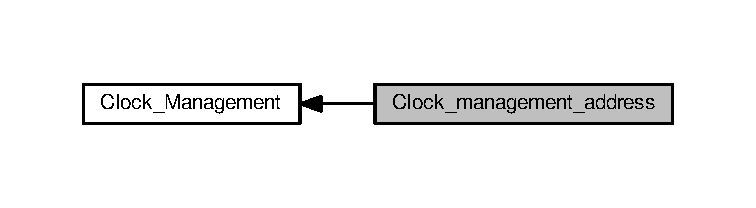
\includegraphics[width=350pt]{d4/d4a/group___clock__management__address}
\end{center}
\end{figure}
\subsection*{Macros}
\begin{DoxyCompactItemize}
\item 
\#define \hyperlink{group___clock__management__address_ga8ee07883213a94b7c2de6f560a3b7073}{T\+I\+M\+E\+\_\+\+B\+A\+S\+E\+\_\+\+A\+D\+D\+R\+E\+SS}~0x00
\item 
\#define \hyperlink{group___clock__management__address_ga31d7b2bb8de218af4333c18718955628}{D\+A\+T\+E\+\_\+\+B\+A\+S\+E\+\_\+\+A\+D\+D\+R\+E\+SS}~0x04
\item 
\#define \hyperlink{group___clock__management__address_gab2393255a8e2127df1aca26ece13641f}{A\+L\+A\+R\+M\+\_\+\+B\+A\+S\+E\+\_\+\+A\+D\+D\+R\+E\+SS}~0x08
\end{DoxyCompactItemize}


\subsection{Detailed Description}


\subsection{Macro Definition Documentation}
\index{Clock\+\_\+management\+\_\+address@{Clock\+\_\+management\+\_\+address}!A\+L\+A\+R\+M\+\_\+\+B\+A\+S\+E\+\_\+\+A\+D\+D\+R\+E\+SS@{A\+L\+A\+R\+M\+\_\+\+B\+A\+S\+E\+\_\+\+A\+D\+D\+R\+E\+SS}}
\index{A\+L\+A\+R\+M\+\_\+\+B\+A\+S\+E\+\_\+\+A\+D\+D\+R\+E\+SS@{A\+L\+A\+R\+M\+\_\+\+B\+A\+S\+E\+\_\+\+A\+D\+D\+R\+E\+SS}!Clock\+\_\+management\+\_\+address@{Clock\+\_\+management\+\_\+address}}
\subsubsection[{\texorpdfstring{A\+L\+A\+R\+M\+\_\+\+B\+A\+S\+E\+\_\+\+A\+D\+D\+R\+E\+SS}{ALARM_BASE_ADDRESS}}]{\setlength{\rightskip}{0pt plus 5cm}\#define A\+L\+A\+R\+M\+\_\+\+B\+A\+S\+E\+\_\+\+A\+D\+D\+R\+E\+SS~0x08}\hypertarget{group___clock__management__address_gab2393255a8e2127df1aca26ece13641f}{}\label{group___clock__management__address_gab2393255a8e2127df1aca26ece13641f}


Definition at line 43 of file clock\+\_\+management.\+h.

\index{Clock\+\_\+management\+\_\+address@{Clock\+\_\+management\+\_\+address}!D\+A\+T\+E\+\_\+\+B\+A\+S\+E\+\_\+\+A\+D\+D\+R\+E\+SS@{D\+A\+T\+E\+\_\+\+B\+A\+S\+E\+\_\+\+A\+D\+D\+R\+E\+SS}}
\index{D\+A\+T\+E\+\_\+\+B\+A\+S\+E\+\_\+\+A\+D\+D\+R\+E\+SS@{D\+A\+T\+E\+\_\+\+B\+A\+S\+E\+\_\+\+A\+D\+D\+R\+E\+SS}!Clock\+\_\+management\+\_\+address@{Clock\+\_\+management\+\_\+address}}
\subsubsection[{\texorpdfstring{D\+A\+T\+E\+\_\+\+B\+A\+S\+E\+\_\+\+A\+D\+D\+R\+E\+SS}{DATE_BASE_ADDRESS}}]{\setlength{\rightskip}{0pt plus 5cm}\#define D\+A\+T\+E\+\_\+\+B\+A\+S\+E\+\_\+\+A\+D\+D\+R\+E\+SS~0x04}\hypertarget{group___clock__management__address_ga31d7b2bb8de218af4333c18718955628}{}\label{group___clock__management__address_ga31d7b2bb8de218af4333c18718955628}


Definition at line 42 of file clock\+\_\+management.\+h.

\index{Clock\+\_\+management\+\_\+address@{Clock\+\_\+management\+\_\+address}!T\+I\+M\+E\+\_\+\+B\+A\+S\+E\+\_\+\+A\+D\+D\+R\+E\+SS@{T\+I\+M\+E\+\_\+\+B\+A\+S\+E\+\_\+\+A\+D\+D\+R\+E\+SS}}
\index{T\+I\+M\+E\+\_\+\+B\+A\+S\+E\+\_\+\+A\+D\+D\+R\+E\+SS@{T\+I\+M\+E\+\_\+\+B\+A\+S\+E\+\_\+\+A\+D\+D\+R\+E\+SS}!Clock\+\_\+management\+\_\+address@{Clock\+\_\+management\+\_\+address}}
\subsubsection[{\texorpdfstring{T\+I\+M\+E\+\_\+\+B\+A\+S\+E\+\_\+\+A\+D\+D\+R\+E\+SS}{TIME_BASE_ADDRESS}}]{\setlength{\rightskip}{0pt plus 5cm}\#define T\+I\+M\+E\+\_\+\+B\+A\+S\+E\+\_\+\+A\+D\+D\+R\+E\+SS~0x00}\hypertarget{group___clock__management__address_ga8ee07883213a94b7c2de6f560a3b7073}{}\label{group___clock__management__address_ga8ee07883213a94b7c2de6f560a3b7073}


Definition at line 41 of file clock\+\_\+management.\+h.


\hypertarget{group___clock__management__alarm__offset}{}\section{Clock\+\_\+management\+\_\+alarm\+\_\+offset}
\label{group___clock__management__alarm__offset}\index{Clock\+\_\+management\+\_\+alarm\+\_\+offset@{Clock\+\_\+management\+\_\+alarm\+\_\+offset}}
Collaboration diagram for Clock\+\_\+management\+\_\+alarm\+\_\+offset\+:\nopagebreak
\begin{figure}[H]
\begin{center}
\leavevmode
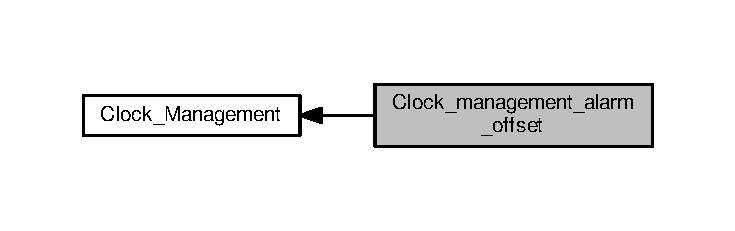
\includegraphics[width=350pt]{de/dc7/group___clock__management__alarm__offset}
\end{center}
\end{figure}
\subsection*{Macros}
\begin{DoxyCompactItemize}
\item 
\#define \hyperlink{group___clock__management__alarm__offset_ga9986a274242ed1976ceb6af6a314e424}{O\+F\+F\+S\+E\+T\+\_\+\+N\+A\+ME}~0x00
\item 
\#define \hyperlink{group___clock__management__alarm__offset_ga4c2226ae357827da27e35a5b27472c80}{O\+F\+F\+S\+E\+T\+\_\+\+D\+A\+T\+E\+W\+E\+E\+K\+D\+AY}~\hyperlink{group___clock__management__constants_ga834e9a379307f869a10f4da078be5786}{N\+A\+M\+E\+\_\+\+S\+I\+ZE}
\item 
\#define \hyperlink{group___clock__management__alarm__offset_ga9eddc8221941f855965c838c15760731}{O\+F\+F\+S\+E\+T\+\_\+\+D\+A\+T\+E\+W\+E\+E\+K\+D\+A\+Y\+\_\+\+S\+EL}~\hyperlink{group___clock__management__alarm__offset_ga4c2226ae357827da27e35a5b27472c80}{O\+F\+F\+S\+E\+T\+\_\+\+D\+A\+T\+E\+W\+E\+E\+K\+D\+AY} + 1
\item 
\#define \hyperlink{group___clock__management__alarm__offset_ga9d6fc23740ab9f37272a3299949d3c11}{O\+F\+F\+S\+E\+T\+\_\+\+M\+A\+SK}~\hyperlink{group___clock__management__alarm__offset_ga9eddc8221941f855965c838c15760731}{O\+F\+F\+S\+E\+T\+\_\+\+D\+A\+T\+E\+W\+E\+E\+K\+D\+A\+Y\+\_\+\+S\+EL} + 4
\item 
\#define \hyperlink{group___clock__management__alarm__offset_ga1153cc94aac429322a110eb8ea996733}{O\+F\+F\+S\+E\+T\+\_\+\+H12}~\hyperlink{group___clock__management__alarm__offset_ga9d6fc23740ab9f37272a3299949d3c11}{O\+F\+F\+S\+E\+T\+\_\+\+M\+A\+SK} + 4
\item 
\#define \hyperlink{group___clock__management__alarm__offset_ga0447fe94b3055242905c1ef82da6ce75}{O\+F\+F\+S\+E\+T\+\_\+\+H\+O\+U\+RS}~\hyperlink{group___clock__management__alarm__offset_ga1153cc94aac429322a110eb8ea996733}{O\+F\+F\+S\+E\+T\+\_\+\+H12} + 1
\item 
\#define \hyperlink{group___clock__management__alarm__offset_gafffbfcb2669e65a487510c041aee5f06}{O\+F\+F\+S\+E\+T\+\_\+\+M\+I\+N\+U\+T\+ES}~\hyperlink{group___clock__management__alarm__offset_ga0447fe94b3055242905c1ef82da6ce75}{O\+F\+F\+S\+E\+T\+\_\+\+H\+O\+U\+RS} + 1
\item 
\#define \hyperlink{group___clock__management__alarm__offset_ga9d48129268662bd4afbc63795d117ba8}{O\+F\+F\+S\+E\+T\+\_\+\+S\+E\+C\+O\+N\+DS}~\hyperlink{group___clock__management__alarm__offset_gafffbfcb2669e65a487510c041aee5f06}{O\+F\+F\+S\+E\+T\+\_\+\+M\+I\+N\+U\+T\+ES} + 1
\end{DoxyCompactItemize}


\subsection{Detailed Description}


\subsection{Macro Definition Documentation}
\index{Clock\+\_\+management\+\_\+alarm\+\_\+offset@{Clock\+\_\+management\+\_\+alarm\+\_\+offset}!O\+F\+F\+S\+E\+T\+\_\+\+D\+A\+T\+E\+W\+E\+E\+K\+D\+AY@{O\+F\+F\+S\+E\+T\+\_\+\+D\+A\+T\+E\+W\+E\+E\+K\+D\+AY}}
\index{O\+F\+F\+S\+E\+T\+\_\+\+D\+A\+T\+E\+W\+E\+E\+K\+D\+AY@{O\+F\+F\+S\+E\+T\+\_\+\+D\+A\+T\+E\+W\+E\+E\+K\+D\+AY}!Clock\+\_\+management\+\_\+alarm\+\_\+offset@{Clock\+\_\+management\+\_\+alarm\+\_\+offset}}
\subsubsection[{\texorpdfstring{O\+F\+F\+S\+E\+T\+\_\+\+D\+A\+T\+E\+W\+E\+E\+K\+D\+AY}{OFFSET_DATEWEEKDAY}}]{\setlength{\rightskip}{0pt plus 5cm}\#define O\+F\+F\+S\+E\+T\+\_\+\+D\+A\+T\+E\+W\+E\+E\+K\+D\+AY~{\bf N\+A\+M\+E\+\_\+\+S\+I\+ZE}}\hypertarget{group___clock__management__alarm__offset_ga4c2226ae357827da27e35a5b27472c80}{}\label{group___clock__management__alarm__offset_ga4c2226ae357827da27e35a5b27472c80}


Definition at line 52 of file clock\+\_\+management.\+h.

\index{Clock\+\_\+management\+\_\+alarm\+\_\+offset@{Clock\+\_\+management\+\_\+alarm\+\_\+offset}!O\+F\+F\+S\+E\+T\+\_\+\+D\+A\+T\+E\+W\+E\+E\+K\+D\+A\+Y\+\_\+\+S\+EL@{O\+F\+F\+S\+E\+T\+\_\+\+D\+A\+T\+E\+W\+E\+E\+K\+D\+A\+Y\+\_\+\+S\+EL}}
\index{O\+F\+F\+S\+E\+T\+\_\+\+D\+A\+T\+E\+W\+E\+E\+K\+D\+A\+Y\+\_\+\+S\+EL@{O\+F\+F\+S\+E\+T\+\_\+\+D\+A\+T\+E\+W\+E\+E\+K\+D\+A\+Y\+\_\+\+S\+EL}!Clock\+\_\+management\+\_\+alarm\+\_\+offset@{Clock\+\_\+management\+\_\+alarm\+\_\+offset}}
\subsubsection[{\texorpdfstring{O\+F\+F\+S\+E\+T\+\_\+\+D\+A\+T\+E\+W\+E\+E\+K\+D\+A\+Y\+\_\+\+S\+EL}{OFFSET_DATEWEEKDAY_SEL}}]{\setlength{\rightskip}{0pt plus 5cm}\#define O\+F\+F\+S\+E\+T\+\_\+\+D\+A\+T\+E\+W\+E\+E\+K\+D\+A\+Y\+\_\+\+S\+EL~{\bf O\+F\+F\+S\+E\+T\+\_\+\+D\+A\+T\+E\+W\+E\+E\+K\+D\+AY} + 1}\hypertarget{group___clock__management__alarm__offset_ga9eddc8221941f855965c838c15760731}{}\label{group___clock__management__alarm__offset_ga9eddc8221941f855965c838c15760731}


Definition at line 53 of file clock\+\_\+management.\+h.

\index{Clock\+\_\+management\+\_\+alarm\+\_\+offset@{Clock\+\_\+management\+\_\+alarm\+\_\+offset}!O\+F\+F\+S\+E\+T\+\_\+\+H12@{O\+F\+F\+S\+E\+T\+\_\+\+H12}}
\index{O\+F\+F\+S\+E\+T\+\_\+\+H12@{O\+F\+F\+S\+E\+T\+\_\+\+H12}!Clock\+\_\+management\+\_\+alarm\+\_\+offset@{Clock\+\_\+management\+\_\+alarm\+\_\+offset}}
\subsubsection[{\texorpdfstring{O\+F\+F\+S\+E\+T\+\_\+\+H12}{OFFSET_H12}}]{\setlength{\rightskip}{0pt plus 5cm}\#define O\+F\+F\+S\+E\+T\+\_\+\+H12~{\bf O\+F\+F\+S\+E\+T\+\_\+\+M\+A\+SK} + 4}\hypertarget{group___clock__management__alarm__offset_ga1153cc94aac429322a110eb8ea996733}{}\label{group___clock__management__alarm__offset_ga1153cc94aac429322a110eb8ea996733}


Definition at line 55 of file clock\+\_\+management.\+h.

\index{Clock\+\_\+management\+\_\+alarm\+\_\+offset@{Clock\+\_\+management\+\_\+alarm\+\_\+offset}!O\+F\+F\+S\+E\+T\+\_\+\+H\+O\+U\+RS@{O\+F\+F\+S\+E\+T\+\_\+\+H\+O\+U\+RS}}
\index{O\+F\+F\+S\+E\+T\+\_\+\+H\+O\+U\+RS@{O\+F\+F\+S\+E\+T\+\_\+\+H\+O\+U\+RS}!Clock\+\_\+management\+\_\+alarm\+\_\+offset@{Clock\+\_\+management\+\_\+alarm\+\_\+offset}}
\subsubsection[{\texorpdfstring{O\+F\+F\+S\+E\+T\+\_\+\+H\+O\+U\+RS}{OFFSET_HOURS}}]{\setlength{\rightskip}{0pt plus 5cm}\#define O\+F\+F\+S\+E\+T\+\_\+\+H\+O\+U\+RS~{\bf O\+F\+F\+S\+E\+T\+\_\+\+H12} + 1}\hypertarget{group___clock__management__alarm__offset_ga0447fe94b3055242905c1ef82da6ce75}{}\label{group___clock__management__alarm__offset_ga0447fe94b3055242905c1ef82da6ce75}


Definition at line 56 of file clock\+\_\+management.\+h.

\index{Clock\+\_\+management\+\_\+alarm\+\_\+offset@{Clock\+\_\+management\+\_\+alarm\+\_\+offset}!O\+F\+F\+S\+E\+T\+\_\+\+M\+A\+SK@{O\+F\+F\+S\+E\+T\+\_\+\+M\+A\+SK}}
\index{O\+F\+F\+S\+E\+T\+\_\+\+M\+A\+SK@{O\+F\+F\+S\+E\+T\+\_\+\+M\+A\+SK}!Clock\+\_\+management\+\_\+alarm\+\_\+offset@{Clock\+\_\+management\+\_\+alarm\+\_\+offset}}
\subsubsection[{\texorpdfstring{O\+F\+F\+S\+E\+T\+\_\+\+M\+A\+SK}{OFFSET_MASK}}]{\setlength{\rightskip}{0pt plus 5cm}\#define O\+F\+F\+S\+E\+T\+\_\+\+M\+A\+SK~{\bf O\+F\+F\+S\+E\+T\+\_\+\+D\+A\+T\+E\+W\+E\+E\+K\+D\+A\+Y\+\_\+\+S\+EL} + 4}\hypertarget{group___clock__management__alarm__offset_ga9d6fc23740ab9f37272a3299949d3c11}{}\label{group___clock__management__alarm__offset_ga9d6fc23740ab9f37272a3299949d3c11}


Definition at line 54 of file clock\+\_\+management.\+h.

\index{Clock\+\_\+management\+\_\+alarm\+\_\+offset@{Clock\+\_\+management\+\_\+alarm\+\_\+offset}!O\+F\+F\+S\+E\+T\+\_\+\+M\+I\+N\+U\+T\+ES@{O\+F\+F\+S\+E\+T\+\_\+\+M\+I\+N\+U\+T\+ES}}
\index{O\+F\+F\+S\+E\+T\+\_\+\+M\+I\+N\+U\+T\+ES@{O\+F\+F\+S\+E\+T\+\_\+\+M\+I\+N\+U\+T\+ES}!Clock\+\_\+management\+\_\+alarm\+\_\+offset@{Clock\+\_\+management\+\_\+alarm\+\_\+offset}}
\subsubsection[{\texorpdfstring{O\+F\+F\+S\+E\+T\+\_\+\+M\+I\+N\+U\+T\+ES}{OFFSET_MINUTES}}]{\setlength{\rightskip}{0pt plus 5cm}\#define O\+F\+F\+S\+E\+T\+\_\+\+M\+I\+N\+U\+T\+ES~{\bf O\+F\+F\+S\+E\+T\+\_\+\+H\+O\+U\+RS} + 1}\hypertarget{group___clock__management__alarm__offset_gafffbfcb2669e65a487510c041aee5f06}{}\label{group___clock__management__alarm__offset_gafffbfcb2669e65a487510c041aee5f06}


Definition at line 57 of file clock\+\_\+management.\+h.

\index{Clock\+\_\+management\+\_\+alarm\+\_\+offset@{Clock\+\_\+management\+\_\+alarm\+\_\+offset}!O\+F\+F\+S\+E\+T\+\_\+\+N\+A\+ME@{O\+F\+F\+S\+E\+T\+\_\+\+N\+A\+ME}}
\index{O\+F\+F\+S\+E\+T\+\_\+\+N\+A\+ME@{O\+F\+F\+S\+E\+T\+\_\+\+N\+A\+ME}!Clock\+\_\+management\+\_\+alarm\+\_\+offset@{Clock\+\_\+management\+\_\+alarm\+\_\+offset}}
\subsubsection[{\texorpdfstring{O\+F\+F\+S\+E\+T\+\_\+\+N\+A\+ME}{OFFSET_NAME}}]{\setlength{\rightskip}{0pt plus 5cm}\#define O\+F\+F\+S\+E\+T\+\_\+\+N\+A\+ME~0x00}\hypertarget{group___clock__management__alarm__offset_ga9986a274242ed1976ceb6af6a314e424}{}\label{group___clock__management__alarm__offset_ga9986a274242ed1976ceb6af6a314e424}


Definition at line 51 of file clock\+\_\+management.\+h.

\index{Clock\+\_\+management\+\_\+alarm\+\_\+offset@{Clock\+\_\+management\+\_\+alarm\+\_\+offset}!O\+F\+F\+S\+E\+T\+\_\+\+S\+E\+C\+O\+N\+DS@{O\+F\+F\+S\+E\+T\+\_\+\+S\+E\+C\+O\+N\+DS}}
\index{O\+F\+F\+S\+E\+T\+\_\+\+S\+E\+C\+O\+N\+DS@{O\+F\+F\+S\+E\+T\+\_\+\+S\+E\+C\+O\+N\+DS}!Clock\+\_\+management\+\_\+alarm\+\_\+offset@{Clock\+\_\+management\+\_\+alarm\+\_\+offset}}
\subsubsection[{\texorpdfstring{O\+F\+F\+S\+E\+T\+\_\+\+S\+E\+C\+O\+N\+DS}{OFFSET_SECONDS}}]{\setlength{\rightskip}{0pt plus 5cm}\#define O\+F\+F\+S\+E\+T\+\_\+\+S\+E\+C\+O\+N\+DS~{\bf O\+F\+F\+S\+E\+T\+\_\+\+M\+I\+N\+U\+T\+ES} + 1}\hypertarget{group___clock__management__alarm__offset_ga9d48129268662bd4afbc63795d117ba8}{}\label{group___clock__management__alarm__offset_ga9d48129268662bd4afbc63795d117ba8}


Definition at line 58 of file clock\+\_\+management.\+h.


\hypertarget{group___clock__management__constants}{}\section{Clock\+\_\+management\+\_\+constants}
\label{group___clock__management__constants}\index{Clock\+\_\+management\+\_\+constants@{Clock\+\_\+management\+\_\+constants}}
Collaboration diagram for Clock\+\_\+management\+\_\+constants\+:\nopagebreak
\begin{figure}[H]
\begin{center}
\leavevmode
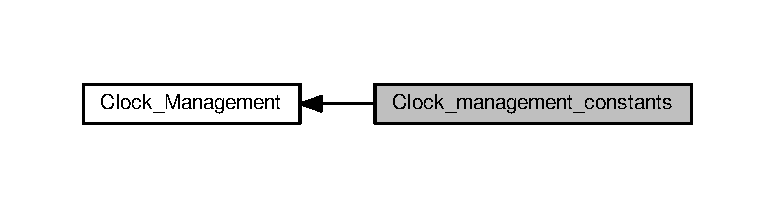
\includegraphics[width=350pt]{d5/db3/group___clock__management__constants}
\end{center}
\end{figure}
\subsection*{Macros}
\begin{DoxyCompactItemize}
\item 
\#define \hyperlink{group___clock__management__constants_ga834e9a379307f869a10f4da078be5786}{N\+A\+M\+E\+\_\+\+S\+I\+ZE}~31
\end{DoxyCompactItemize}


\subsection{Detailed Description}


\subsection{Macro Definition Documentation}
\index{Clock\+\_\+management\+\_\+constants@{Clock\+\_\+management\+\_\+constants}!N\+A\+M\+E\+\_\+\+S\+I\+ZE@{N\+A\+M\+E\+\_\+\+S\+I\+ZE}}
\index{N\+A\+M\+E\+\_\+\+S\+I\+ZE@{N\+A\+M\+E\+\_\+\+S\+I\+ZE}!Clock\+\_\+management\+\_\+constants@{Clock\+\_\+management\+\_\+constants}}
\subsubsection[{\texorpdfstring{N\+A\+M\+E\+\_\+\+S\+I\+ZE}{NAME_SIZE}}]{\setlength{\rightskip}{0pt plus 5cm}\#define N\+A\+M\+E\+\_\+\+S\+I\+ZE~31}\hypertarget{group___clock__management__constants_ga834e9a379307f869a10f4da078be5786}{}\label{group___clock__management__constants_ga834e9a379307f869a10f4da078be5786}


Definition at line 66 of file clock\+\_\+management.\+h.


\hypertarget{group__clock__management}{}\section{variables}
\label{group__clock__management}\index{variables@{variables}}
Collaboration diagram for variables\+:\nopagebreak
\begin{figure}[H]
\begin{center}
\leavevmode
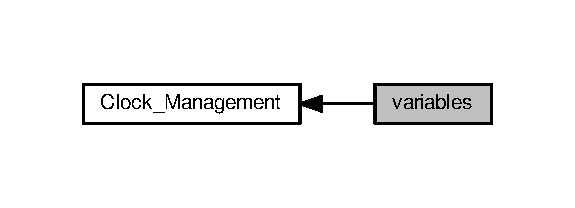
\includegraphics[width=276pt]{d9/dfc/group__clock__management}
\end{center}
\end{figure}
\subsection*{Variables}
\begin{DoxyCompactItemize}
\item 
uint16\+\_\+t \hyperlink{group__clock__management_gadafaa69421576ac611d507121be2e8f2}{eeprom\+\_\+index}
\item 
uint16\+\_\+t \hyperlink{group__clock__management_gaae2a6d57125e1b394a897958b141986b}{next\+\_\+alarm}
\end{DoxyCompactItemize}


\subsection{Detailed Description}


\subsection{Variable Documentation}
\index{variables@{variables}!eeprom\+\_\+index@{eeprom\+\_\+index}}
\index{eeprom\+\_\+index@{eeprom\+\_\+index}!variables@{variables}}
\subsubsection[{\texorpdfstring{eeprom\+\_\+index}{eeprom_index}}]{\setlength{\rightskip}{0pt plus 5cm}uint16\+\_\+t eeprom\+\_\+index}\hypertarget{group__clock__management_gadafaa69421576ac611d507121be2e8f2}{}\label{group__clock__management_gadafaa69421576ac611d507121be2e8f2}
\index{variables@{variables}!next\+\_\+alarm@{next\+\_\+alarm}}
\index{next\+\_\+alarm@{next\+\_\+alarm}!variables@{variables}}
\subsubsection[{\texorpdfstring{next\+\_\+alarm}{next_alarm}}]{\setlength{\rightskip}{0pt plus 5cm}uint16\+\_\+t next\+\_\+alarm}\hypertarget{group__clock__management_gaae2a6d57125e1b394a897958b141986b}{}\label{group__clock__management_gaae2a6d57125e1b394a897958b141986b}

\hypertarget{group__type}{}\section{Type}
\label{group__type}\index{Type@{Type}}


Alarm type.  


Collaboration diagram for Type\+:\nopagebreak
\begin{figure}[H]
\begin{center}
\leavevmode
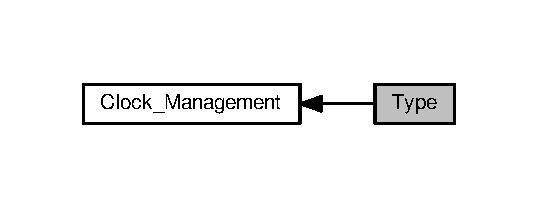
\includegraphics[width=258pt]{dd/d8f/group__type}
\end{center}
\end{figure}
\subsection*{Data Structures}
\begin{DoxyCompactItemize}
\item 
struct \hyperlink{group__type_d4/d90/struct_alarm___definition}{Alarm\+\_\+\+Definition}
\end{DoxyCompactItemize}


\subsection{Detailed Description}
Alarm type. 



\subsection{Data Structure Documentation}
\index{Alarm\+\_\+\+Definition@{Alarm\+\_\+\+Definition}}\label{struct_alarm___definition}
\hypertarget{group__type_struct_alarm___definition}{}
\subsubsection{struct Alarm\+\_\+\+Definition}


Definition at line 86 of file clock\+\_\+management.\+h.

\begin{DoxyFields}{Data Fields}
char\hypertarget{group__type_a69a8bc4ad7884ca26f0c942d5ef3f430}{}\label{group__type_a69a8bc4ad7884ca26f0c942d5ef3f430}
&
alarm\+Name\mbox{[}\hyperlink{group___clock__management__constants_ga834e9a379307f869a10f4da078be5786}{N\+A\+M\+E\+\_\+\+S\+I\+ZE}\mbox{]}&
\\
\hline

R\+T\+C\+\_\+\+Alarm\+Type\+Def\hypertarget{group__type_aec96eda8f1baa300f50a7ef3d8a9f342}{}\label{group__type_aec96eda8f1baa300f50a7ef3d8a9f342}
&
alarm\+Parameters&
\\
\hline

\end{DoxyFields}

\hypertarget{group___clock___management___eeprom}{}\section{Clock\+\_\+\+Management\+\_\+\+Eeprom}
\label{group___clock___management___eeprom}\index{Clock\+\_\+\+Management\+\_\+\+Eeprom@{Clock\+\_\+\+Management\+\_\+\+Eeprom}}


Saving and Loading of clock information.  


Collaboration diagram for Clock\+\_\+\+Management\+\_\+\+Eeprom\+:\nopagebreak
\begin{figure}[H]
\begin{center}
\leavevmode
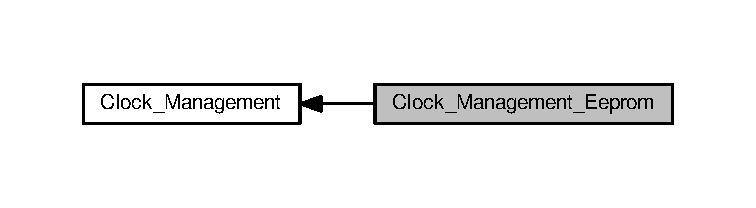
\includegraphics[width=350pt]{df/d13/group___clock___management___eeprom}
\end{center}
\end{figure}
\subsection*{Functions}
\begin{DoxyCompactItemize}
\item 
Error\+Status \hyperlink{group___clock___management___eeprom_ga98aa8b6a9e96cd5fd883602c23bf1c4a}{Clock\+Management\+\_\+save\+Alarm} (\hyperlink{group__type_d4/d90/struct_alarm___definition}{Alarm\+\_\+\+Definition} $\ast$Alarm\+\_\+\+Def, uint16\+\_\+t address)
\begin{DoxyCompactList}\small\item\em Save an alarm settings to eeprom. \end{DoxyCompactList}\item 
Error\+Status \hyperlink{group___clock___management___eeprom_ga4d1c66f7ce4d69b6903471823ab105f7}{Clock\+Management\+\_\+save\+Time} (R\+T\+C\+\_\+\+Time\+Type\+Def $\ast$Time\+\_\+\+Def)
\begin{DoxyCompactList}\small\item\em Save the time settings to eeprom. \end{DoxyCompactList}\item 
Error\+Status \hyperlink{group___clock___management___eeprom_ga32f8e9df4e2b14dfa0db0300437fe335}{Clock\+Management\+\_\+save\+Date} (R\+T\+C\+\_\+\+Date\+Type\+Def $\ast$Date\+\_\+\+Def)
\begin{DoxyCompactList}\small\item\em Save the date settings to eeprom. \end{DoxyCompactList}\item 
\hyperlink{group__type_d4/d90/struct_alarm___definition}{Alarm\+\_\+\+Definition} \hyperlink{group___clock___management___eeprom_gab8401f24d519d3a2e54c3ba5dab80376}{Clock\+Management\+\_\+load\+Alarm} (uint16\+\_\+t index)
\begin{DoxyCompactList}\small\item\em load an alarm settings from eeprom \end{DoxyCompactList}\item 
R\+T\+C\+\_\+\+Time\+Type\+Def \hyperlink{group___clock___management___eeprom_ga166e0bbb5e934cc45657ffad06ff1d62}{Clock\+Management\+\_\+load\+Time} (void)
\begin{DoxyCompactList}\small\item\em Load the time settings from eeprom. \end{DoxyCompactList}\item 
R\+T\+C\+\_\+\+Date\+Type\+Def \hyperlink{group___clock___management___eeprom_ga3980560a99803ef94287127ff3157f91}{Clock\+Management\+\_\+load\+Date} (void)
\begin{DoxyCompactList}\small\item\em Load the date settings from eeprom. \end{DoxyCompactList}\end{DoxyCompactItemize}


\subsection{Detailed Description}
Saving and Loading of clock information. 

\begin{DoxyVerb}===============================================================================
       ##### Clock Management: Eeprom date, time, and alarm access #####
===============================================================================
\end{DoxyVerb}
 

\subsection{Function Documentation}
\index{Clock\+\_\+\+Management\+\_\+\+Eeprom@{Clock\+\_\+\+Management\+\_\+\+Eeprom}!Clock\+Management\+\_\+load\+Alarm@{Clock\+Management\+\_\+load\+Alarm}}
\index{Clock\+Management\+\_\+load\+Alarm@{Clock\+Management\+\_\+load\+Alarm}!Clock\+\_\+\+Management\+\_\+\+Eeprom@{Clock\+\_\+\+Management\+\_\+\+Eeprom}}
\subsubsection[{\texorpdfstring{Clock\+Management\+\_\+load\+Alarm(uint16\+\_\+t index)}{ClockManagement_loadAlarm(uint16_t index)}}]{\setlength{\rightskip}{0pt plus 5cm}{\bf Alarm\+\_\+\+Definition} Clock\+Management\+\_\+load\+Alarm (
\begin{DoxyParamCaption}
\item[{uint16\+\_\+t}]{index}
\end{DoxyParamCaption}
)}\hypertarget{group___clock___management___eeprom_gab8401f24d519d3a2e54c3ba5dab80376}{}\label{group___clock___management___eeprom_gab8401f24d519d3a2e54c3ba5dab80376}


load an alarm settings from eeprom 

\begin{DoxyNote}{Note}
Load in this order\+: Name, Date\+Week\+Day, Date\+Week\+Day\+Sel, Mask H12, Hours, Minutes, Seconds 
\end{DoxyNote}

\begin{DoxyParams}{Parameters}
{\em index} & the index in memory of the alarm \\
\hline
\end{DoxyParams}

\begin{DoxyRetVals}{Return values}
{\em \hyperlink{group__type_d4/d90/struct_alarm___definition}{Alarm\+\_\+\+Definition}} & \\
\hline
\end{DoxyRetVals}


Definition at line 103 of file clock\+\_\+management.\+c.



Here is the call graph for this function\+:
\nopagebreak
\begin{figure}[H]
\begin{center}
\leavevmode
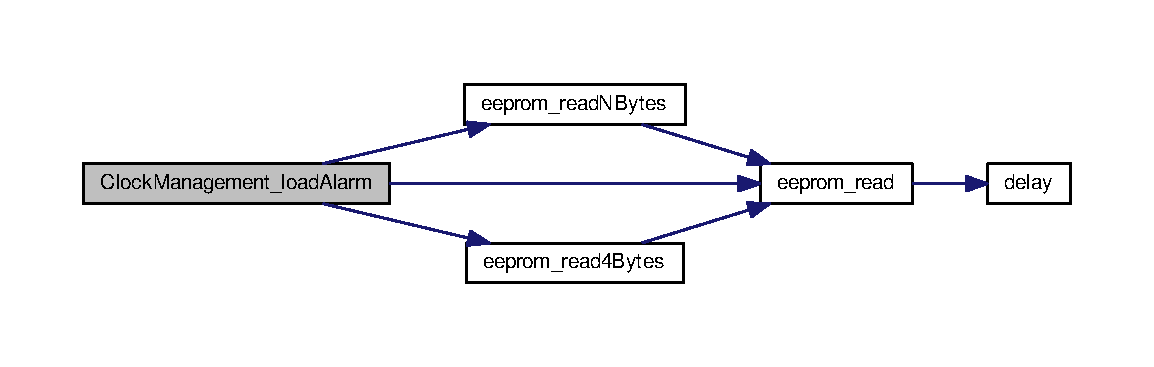
\includegraphics[width=350pt]{df/d13/group___clock___management___eeprom_gab8401f24d519d3a2e54c3ba5dab80376_cgraph}
\end{center}
\end{figure}




Here is the caller graph for this function\+:\nopagebreak
\begin{figure}[H]
\begin{center}
\leavevmode
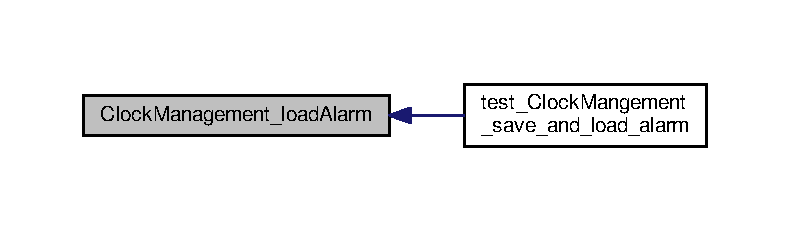
\includegraphics[width=350pt]{df/d13/group___clock___management___eeprom_gab8401f24d519d3a2e54c3ba5dab80376_icgraph}
\end{center}
\end{figure}


\index{Clock\+\_\+\+Management\+\_\+\+Eeprom@{Clock\+\_\+\+Management\+\_\+\+Eeprom}!Clock\+Management\+\_\+load\+Date@{Clock\+Management\+\_\+load\+Date}}
\index{Clock\+Management\+\_\+load\+Date@{Clock\+Management\+\_\+load\+Date}!Clock\+\_\+\+Management\+\_\+\+Eeprom@{Clock\+\_\+\+Management\+\_\+\+Eeprom}}
\subsubsection[{\texorpdfstring{Clock\+Management\+\_\+load\+Date(void)}{ClockManagement_loadDate(void)}}]{\setlength{\rightskip}{0pt plus 5cm}R\+T\+C\+\_\+\+Date\+Type\+Def Clock\+Management\+\_\+load\+Date (
\begin{DoxyParamCaption}
\item[{void}]{}
\end{DoxyParamCaption}
)}\hypertarget{group___clock___management___eeprom_ga3980560a99803ef94287127ff3157f91}{}\label{group___clock___management___eeprom_ga3980560a99803ef94287127ff3157f91}


Load the date settings from eeprom. 

\begin{DoxyNote}{Note}
Load Date, Month, Week\+Day, and Year in that order 
\end{DoxyNote}

\begin{DoxyParams}{Parameters}
{\em None} & \\
\hline
\end{DoxyParams}

\begin{DoxyRetVals}{Return values}
{\em R\+T\+C\+\_\+\+Date\+Type\+Def} & \\
\hline
\end{DoxyRetVals}


Definition at line 139 of file clock\+\_\+management.\+c.



Here is the call graph for this function\+:\nopagebreak
\begin{figure}[H]
\begin{center}
\leavevmode
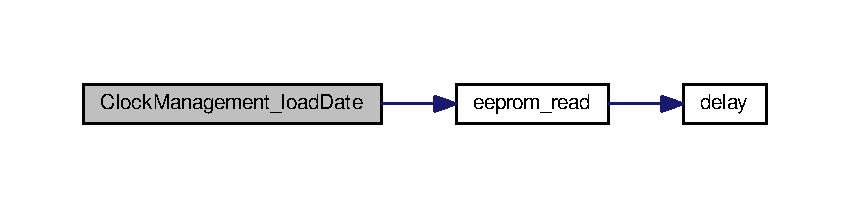
\includegraphics[width=350pt]{df/d13/group___clock___management___eeprom_ga3980560a99803ef94287127ff3157f91_cgraph}
\end{center}
\end{figure}




Here is the caller graph for this function\+:\nopagebreak
\begin{figure}[H]
\begin{center}
\leavevmode
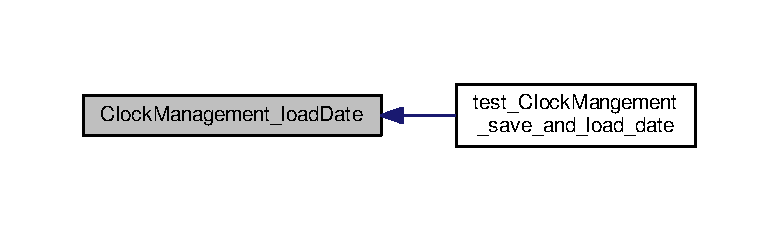
\includegraphics[width=350pt]{df/d13/group___clock___management___eeprom_ga3980560a99803ef94287127ff3157f91_icgraph}
\end{center}
\end{figure}


\index{Clock\+\_\+\+Management\+\_\+\+Eeprom@{Clock\+\_\+\+Management\+\_\+\+Eeprom}!Clock\+Management\+\_\+load\+Time@{Clock\+Management\+\_\+load\+Time}}
\index{Clock\+Management\+\_\+load\+Time@{Clock\+Management\+\_\+load\+Time}!Clock\+\_\+\+Management\+\_\+\+Eeprom@{Clock\+\_\+\+Management\+\_\+\+Eeprom}}
\subsubsection[{\texorpdfstring{Clock\+Management\+\_\+load\+Time(void)}{ClockManagement_loadTime(void)}}]{\setlength{\rightskip}{0pt plus 5cm}R\+T\+C\+\_\+\+Time\+Type\+Def Clock\+Management\+\_\+load\+Time (
\begin{DoxyParamCaption}
\item[{void}]{}
\end{DoxyParamCaption}
)}\hypertarget{group___clock___management___eeprom_ga166e0bbb5e934cc45657ffad06ff1d62}{}\label{group___clock___management___eeprom_ga166e0bbb5e934cc45657ffad06ff1d62}


Load the time settings from eeprom. 

\begin{DoxyNote}{Note}
Load H12, Hours, Minutes, and Seconds in that order 
\end{DoxyNote}

\begin{DoxyParams}{Parameters}
{\em None} & \\
\hline
\end{DoxyParams}

\begin{DoxyRetVals}{Return values}
{\em R\+T\+C\+\_\+\+Time\+Type\+Def} & \\
\hline
\end{DoxyRetVals}


Definition at line 123 of file clock\+\_\+management.\+c.



Here is the call graph for this function\+:\nopagebreak
\begin{figure}[H]
\begin{center}
\leavevmode
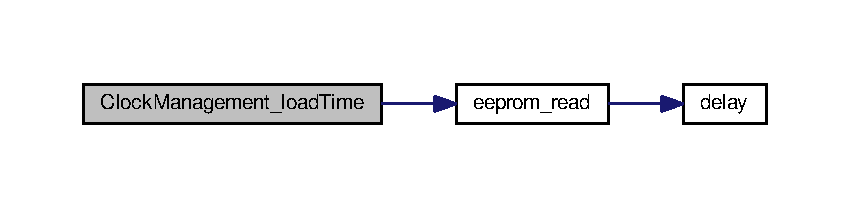
\includegraphics[width=350pt]{df/d13/group___clock___management___eeprom_ga166e0bbb5e934cc45657ffad06ff1d62_cgraph}
\end{center}
\end{figure}




Here is the caller graph for this function\+:\nopagebreak
\begin{figure}[H]
\begin{center}
\leavevmode
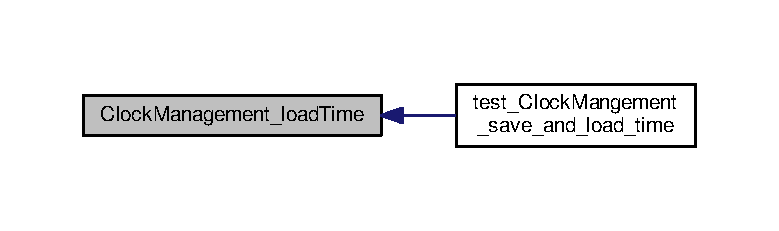
\includegraphics[width=350pt]{df/d13/group___clock___management___eeprom_ga166e0bbb5e934cc45657ffad06ff1d62_icgraph}
\end{center}
\end{figure}


\index{Clock\+\_\+\+Management\+\_\+\+Eeprom@{Clock\+\_\+\+Management\+\_\+\+Eeprom}!Clock\+Management\+\_\+save\+Alarm@{Clock\+Management\+\_\+save\+Alarm}}
\index{Clock\+Management\+\_\+save\+Alarm@{Clock\+Management\+\_\+save\+Alarm}!Clock\+\_\+\+Management\+\_\+\+Eeprom@{Clock\+\_\+\+Management\+\_\+\+Eeprom}}
\subsubsection[{\texorpdfstring{Clock\+Management\+\_\+save\+Alarm(\+Alarm\+\_\+\+Definition $\ast$\+Alarm\+\_\+\+Def, uint16\+\_\+t address)}{ClockManagement_saveAlarm(Alarm_Definition *Alarm_Def, uint16_t address)}}]{\setlength{\rightskip}{0pt plus 5cm}Error\+Status Clock\+Management\+\_\+save\+Alarm (
\begin{DoxyParamCaption}
\item[{{\bf Alarm\+\_\+\+Definition} $\ast$}]{Alarm\+\_\+\+Def, }
\item[{uint16\+\_\+t}]{address}
\end{DoxyParamCaption}
)}\hypertarget{group___clock___management___eeprom_ga98aa8b6a9e96cd5fd883602c23bf1c4a}{}\label{group___clock___management___eeprom_ga98aa8b6a9e96cd5fd883602c23bf1c4a}


Save an alarm settings to eeprom. 

\begin{DoxyNote}{Note}
Save in this order\+: Name, Date\+Week\+Dat, Date\+Week\+Day\+Sel, Mask H12, Hours, Minutes, Seconds 
\end{DoxyNote}

\begin{DoxyParams}{Parameters}
{\em Alarm\+\_\+\+Def} & the alarm setitngs \\
\hline
\end{DoxyParams}

\begin{DoxyRetVals}{Return values}
{\em Error\+Status} & \\
\hline
\end{DoxyRetVals}


Definition at line 57 of file clock\+\_\+management.\+c.



Here is the call graph for this function\+:\nopagebreak
\begin{figure}[H]
\begin{center}
\leavevmode
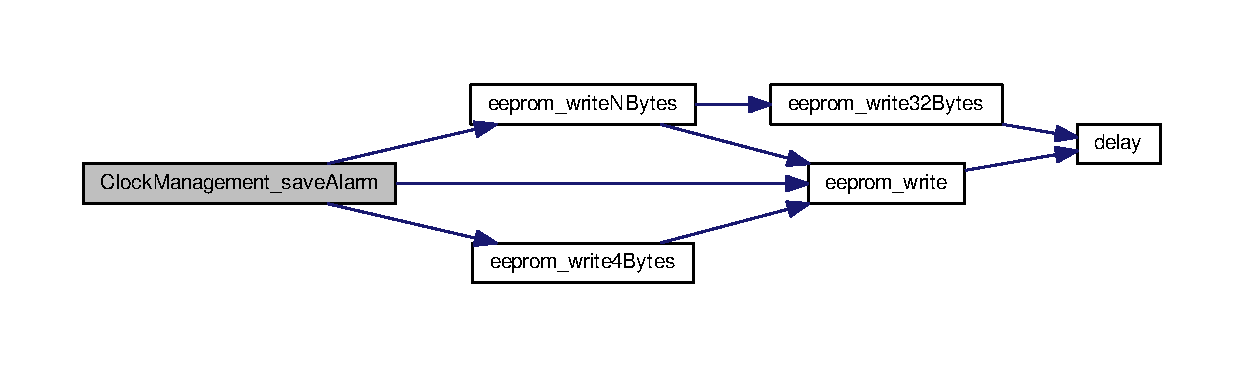
\includegraphics[width=350pt]{df/d13/group___clock___management___eeprom_ga98aa8b6a9e96cd5fd883602c23bf1c4a_cgraph}
\end{center}
\end{figure}




Here is the caller graph for this function\+:\nopagebreak
\begin{figure}[H]
\begin{center}
\leavevmode
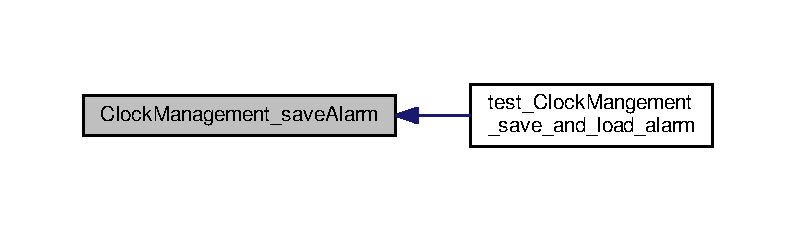
\includegraphics[width=350pt]{df/d13/group___clock___management___eeprom_ga98aa8b6a9e96cd5fd883602c23bf1c4a_icgraph}
\end{center}
\end{figure}


\index{Clock\+\_\+\+Management\+\_\+\+Eeprom@{Clock\+\_\+\+Management\+\_\+\+Eeprom}!Clock\+Management\+\_\+save\+Date@{Clock\+Management\+\_\+save\+Date}}
\index{Clock\+Management\+\_\+save\+Date@{Clock\+Management\+\_\+save\+Date}!Clock\+\_\+\+Management\+\_\+\+Eeprom@{Clock\+\_\+\+Management\+\_\+\+Eeprom}}
\subsubsection[{\texorpdfstring{Clock\+Management\+\_\+save\+Date(\+R\+T\+C\+\_\+\+Date\+Type\+Def $\ast$\+Date\+\_\+\+Def)}{ClockManagement_saveDate(RTC_DateTypeDef *Date_Def)}}]{\setlength{\rightskip}{0pt plus 5cm}Error\+Status Clock\+Management\+\_\+save\+Date (
\begin{DoxyParamCaption}
\item[{R\+T\+C\+\_\+\+Date\+Type\+Def $\ast$}]{Date\+\_\+\+Def}
\end{DoxyParamCaption}
)}\hypertarget{group___clock___management___eeprom_ga32f8e9df4e2b14dfa0db0300437fe335}{}\label{group___clock___management___eeprom_ga32f8e9df4e2b14dfa0db0300437fe335}


Save the date settings to eeprom. 

\begin{DoxyNote}{Note}
Save Date, Month, Week\+Day, and Year in that order 
\end{DoxyNote}

\begin{DoxyParams}{Parameters}
{\em Date\+\_\+\+Def} & the date setitngs \\
\hline
\end{DoxyParams}

\begin{DoxyRetVals}{Return values}
{\em Error\+Status} & \\
\hline
\end{DoxyRetVals}


Definition at line 89 of file clock\+\_\+management.\+c.



Here is the call graph for this function\+:\nopagebreak
\begin{figure}[H]
\begin{center}
\leavevmode
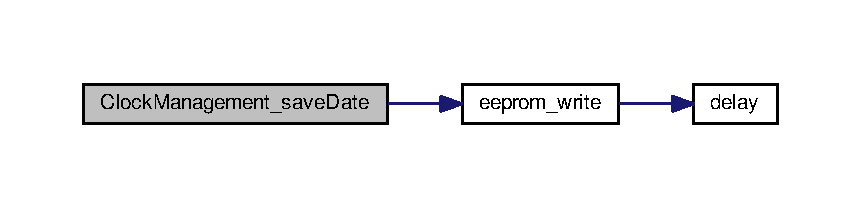
\includegraphics[width=350pt]{df/d13/group___clock___management___eeprom_ga32f8e9df4e2b14dfa0db0300437fe335_cgraph}
\end{center}
\end{figure}




Here is the caller graph for this function\+:\nopagebreak
\begin{figure}[H]
\begin{center}
\leavevmode
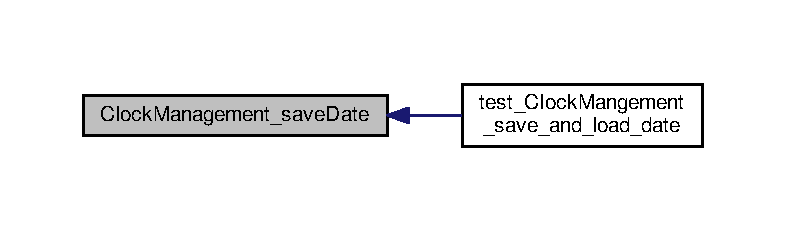
\includegraphics[width=350pt]{df/d13/group___clock___management___eeprom_ga32f8e9df4e2b14dfa0db0300437fe335_icgraph}
\end{center}
\end{figure}


\index{Clock\+\_\+\+Management\+\_\+\+Eeprom@{Clock\+\_\+\+Management\+\_\+\+Eeprom}!Clock\+Management\+\_\+save\+Time@{Clock\+Management\+\_\+save\+Time}}
\index{Clock\+Management\+\_\+save\+Time@{Clock\+Management\+\_\+save\+Time}!Clock\+\_\+\+Management\+\_\+\+Eeprom@{Clock\+\_\+\+Management\+\_\+\+Eeprom}}
\subsubsection[{\texorpdfstring{Clock\+Management\+\_\+save\+Time(\+R\+T\+C\+\_\+\+Time\+Type\+Def $\ast$\+Time\+\_\+\+Def)}{ClockManagement_saveTime(RTC_TimeTypeDef *Time_Def)}}]{\setlength{\rightskip}{0pt plus 5cm}Error\+Status Clock\+Management\+\_\+save\+Time (
\begin{DoxyParamCaption}
\item[{R\+T\+C\+\_\+\+Time\+Type\+Def $\ast$}]{Time\+\_\+\+Def}
\end{DoxyParamCaption}
)}\hypertarget{group___clock___management___eeprom_ga4d1c66f7ce4d69b6903471823ab105f7}{}\label{group___clock___management___eeprom_ga4d1c66f7ce4d69b6903471823ab105f7}


Save the time settings to eeprom. 

\begin{DoxyNote}{Note}
Save H12, Hours, Minutes, and Seconds in that order 
\end{DoxyNote}

\begin{DoxyParams}{Parameters}
{\em Time\+\_\+\+Def} & the time setitngs \\
\hline
\end{DoxyParams}

\begin{DoxyRetVals}{Return values}
{\em Error\+Status} & \\
\hline
\end{DoxyRetVals}


Definition at line 75 of file clock\+\_\+management.\+c.



Here is the call graph for this function\+:\nopagebreak
\begin{figure}[H]
\begin{center}
\leavevmode
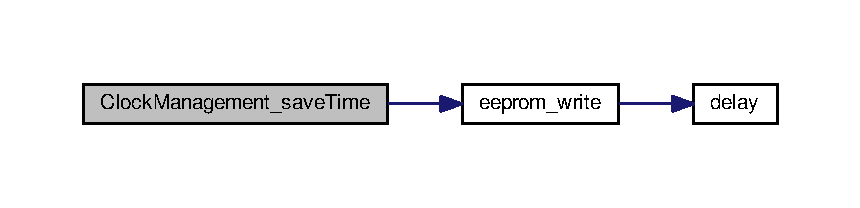
\includegraphics[width=350pt]{df/d13/group___clock___management___eeprom_ga4d1c66f7ce4d69b6903471823ab105f7_cgraph}
\end{center}
\end{figure}




Here is the caller graph for this function\+:\nopagebreak
\begin{figure}[H]
\begin{center}
\leavevmode
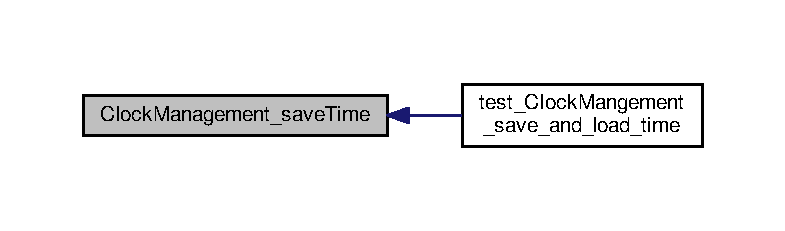
\includegraphics[width=350pt]{df/d13/group___clock___management___eeprom_ga4d1c66f7ce4d69b6903471823ab105f7_icgraph}
\end{center}
\end{figure}



\hypertarget{group___clock___management___alarm_comp}{}\section{Clock\+\_\+\+Management\+\_\+\+Alarm\+Comp}
\label{group___clock___management___alarm_comp}\index{Clock\+\_\+\+Management\+\_\+\+Alarm\+Comp@{Clock\+\_\+\+Management\+\_\+\+Alarm\+Comp}}


Comparison between dates, times and alarms.  


Collaboration diagram for Clock\+\_\+\+Management\+\_\+\+Alarm\+Comp\+:
% FIG 0
\subsection*{Functions}
\begin{DoxyCompactItemize}
\item 
uint32\+\_\+t \hyperlink{group___clock___management___alarm_comp_ga6e567ef31c1220b3440ca3f726f86d10}{Clock\+Management\+\_\+alarm2int} (\hyperlink{struct_alarm___definition}{Alarm\+\_\+\+Definition} $\ast$alarm)
\begin{DoxyCompactList}\small\item\em Convert an alarm to an integer. \end{DoxyCompactList}\item 
uint32\+\_\+t \hyperlink{group___clock___management___alarm_comp_ga36a1b1fbb98de2b2b73ccb40e87e4518}{Clock\+Management\+\_\+time2int} (\hyperlink{struct_alarm___definition}{Alarm\+\_\+\+Definition} $\ast$time)
\begin{DoxyCompactList}\small\item\em Convert a time to an integer. \end{DoxyCompactList}\item 
uint32\+\_\+t \hyperlink{group___clock___management___alarm_comp_ga9e3b465b980b97aa4477ac3574b5cfba}{Clock\+Management\+\_\+date2int} (\hyperlink{struct_alarm___definition}{Alarm\+\_\+\+Definition} $\ast$date)
\begin{DoxyCompactList}\small\item\em Convert an date to an integer. \end{DoxyCompactList}\item 
bool \hyperlink{group___clock___management___alarm_comp_ga20358c9f73302a285a8f084823e8eb2f}{Clock\+Management\+\_\+is\+Alarm\+Sooner\+Than} (\hyperlink{struct_alarm___definition}{Alarm\+\_\+\+Definition} alarm1, \hyperlink{struct_alarm___definition}{Alarm\+\_\+\+Definition} alarm2)
\begin{DoxyCompactList}\small\item\em Compare two alarm. \end{DoxyCompactList}\end{DoxyCompactItemize}


\subsection{Detailed Description}
Comparison between dates, times and alarms. 

\begin{DoxyVerb}===============================================================================
       ##### Clock Management: Time, Date, and Alarm comparison #####
===============================================================================
\end{DoxyVerb}
 

\subsection{Function Documentation}
\mbox{\Hypertarget{group___clock___management___alarm_comp_ga6e567ef31c1220b3440ca3f726f86d10}\label{group___clock___management___alarm_comp_ga6e567ef31c1220b3440ca3f726f86d10}} 
\index{Clock\+\_\+\+Management\+\_\+\+Alarm\+Comp@{Clock\+\_\+\+Management\+\_\+\+Alarm\+Comp}!Clock\+Management\+\_\+alarm2int@{Clock\+Management\+\_\+alarm2int}}
\index{Clock\+Management\+\_\+alarm2int@{Clock\+Management\+\_\+alarm2int}!Clock\+\_\+\+Management\+\_\+\+Alarm\+Comp@{Clock\+\_\+\+Management\+\_\+\+Alarm\+Comp}}
\subsubsection{\texorpdfstring{Clock\+Management\+\_\+alarm2int()}{ClockManagement\_alarm2int()}}
{\footnotesize\ttfamily uint32\+\_\+t Clock\+Management\+\_\+alarm2int (\begin{DoxyParamCaption}\item[{\hyperlink{struct_alarm___definition}{Alarm\+\_\+\+Definition} $\ast$}]{alarm }\end{DoxyParamCaption})}



Convert an alarm to an integer. 


\begin{DoxyParams}{Parameters}
{\em alarm} & \\
\hline
\end{DoxyParams}

\begin{DoxyRetVals}{Return values}
{\em uint32\+\_\+t} & representing the alarm \\
\hline
\end{DoxyRetVals}
\mbox{\Hypertarget{group___clock___management___alarm_comp_ga9e3b465b980b97aa4477ac3574b5cfba}\label{group___clock___management___alarm_comp_ga9e3b465b980b97aa4477ac3574b5cfba}} 
\index{Clock\+\_\+\+Management\+\_\+\+Alarm\+Comp@{Clock\+\_\+\+Management\+\_\+\+Alarm\+Comp}!Clock\+Management\+\_\+date2int@{Clock\+Management\+\_\+date2int}}
\index{Clock\+Management\+\_\+date2int@{Clock\+Management\+\_\+date2int}!Clock\+\_\+\+Management\+\_\+\+Alarm\+Comp@{Clock\+\_\+\+Management\+\_\+\+Alarm\+Comp}}
\subsubsection{\texorpdfstring{Clock\+Management\+\_\+date2int()}{ClockManagement\_date2int()}}
{\footnotesize\ttfamily uint32\+\_\+t Clock\+Management\+\_\+date2int (\begin{DoxyParamCaption}\item[{\hyperlink{struct_alarm___definition}{Alarm\+\_\+\+Definition} $\ast$}]{date }\end{DoxyParamCaption})}



Convert an date to an integer. 


\begin{DoxyParams}{Parameters}
{\em date} & \\
\hline
\end{DoxyParams}

\begin{DoxyRetVals}{Return values}
{\em uint32\+\_\+t} & representing the date \\
\hline
\end{DoxyRetVals}
\mbox{\Hypertarget{group___clock___management___alarm_comp_ga20358c9f73302a285a8f084823e8eb2f}\label{group___clock___management___alarm_comp_ga20358c9f73302a285a8f084823e8eb2f}} 
\index{Clock\+\_\+\+Management\+\_\+\+Alarm\+Comp@{Clock\+\_\+\+Management\+\_\+\+Alarm\+Comp}!Clock\+Management\+\_\+is\+Alarm\+Sooner\+Than@{Clock\+Management\+\_\+is\+Alarm\+Sooner\+Than}}
\index{Clock\+Management\+\_\+is\+Alarm\+Sooner\+Than@{Clock\+Management\+\_\+is\+Alarm\+Sooner\+Than}!Clock\+\_\+\+Management\+\_\+\+Alarm\+Comp@{Clock\+\_\+\+Management\+\_\+\+Alarm\+Comp}}
\subsubsection{\texorpdfstring{Clock\+Management\+\_\+is\+Alarm\+Sooner\+Than()}{ClockManagement\_isAlarmSoonerThan()}}
{\footnotesize\ttfamily bool Clock\+Management\+\_\+is\+Alarm\+Sooner\+Than (\begin{DoxyParamCaption}\item[{\hyperlink{struct_alarm___definition}{Alarm\+\_\+\+Definition}}]{alarm1,  }\item[{\hyperlink{struct_alarm___definition}{Alarm\+\_\+\+Definition}}]{alarm2 }\end{DoxyParamCaption})}



Compare two alarm. 


\begin{DoxyParams}{Parameters}
{\em alarm1} & the reference alarm \\
\hline
{\em alarm2} & \\
\hline
\end{DoxyParams}

\begin{DoxyRetVals}{Return values}
{\em uint32\+\_\+t} & representing the time \\
\hline
\end{DoxyRetVals}
\mbox{\Hypertarget{group___clock___management___alarm_comp_ga36a1b1fbb98de2b2b73ccb40e87e4518}\label{group___clock___management___alarm_comp_ga36a1b1fbb98de2b2b73ccb40e87e4518}} 
\index{Clock\+\_\+\+Management\+\_\+\+Alarm\+Comp@{Clock\+\_\+\+Management\+\_\+\+Alarm\+Comp}!Clock\+Management\+\_\+time2int@{Clock\+Management\+\_\+time2int}}
\index{Clock\+Management\+\_\+time2int@{Clock\+Management\+\_\+time2int}!Clock\+\_\+\+Management\+\_\+\+Alarm\+Comp@{Clock\+\_\+\+Management\+\_\+\+Alarm\+Comp}}
\subsubsection{\texorpdfstring{Clock\+Management\+\_\+time2int()}{ClockManagement\_time2int()}}
{\footnotesize\ttfamily uint32\+\_\+t Clock\+Management\+\_\+time2int (\begin{DoxyParamCaption}\item[{\hyperlink{struct_alarm___definition}{Alarm\+\_\+\+Definition} $\ast$}]{time }\end{DoxyParamCaption})}



Convert a time to an integer. 


\begin{DoxyParams}{Parameters}
{\em time} & \\
\hline
\end{DoxyParams}

\begin{DoxyRetVals}{Return values}
{\em uint32\+\_\+t} & representing the time \\
\hline
\end{DoxyRetVals}

\hypertarget{group___clock___management___alarm_update}{}\section{Clock\+\_\+\+Management\+\_\+\+Alarm\+Update}
\label{group___clock___management___alarm_update}\index{Clock\+\_\+\+Management\+\_\+\+Alarm\+Update@{Clock\+\_\+\+Management\+\_\+\+Alarm\+Update}}


Manages updates of alarms and alarm parameters.  


Collaboration diagram for Clock\+\_\+\+Management\+\_\+\+Alarm\+Update\+:
% FIG 0
\subsection*{Functions}
\begin{DoxyCompactItemize}
\item 
\mbox{\Hypertarget{group___clock___management___alarm_update_gab3193e7c0f26b76a48829295caf4888f}\label{group___clock___management___alarm_update_gab3193e7c0f26b76a48829295caf4888f}} 
void \hyperlink{group___clock___management___alarm_update_gab3193e7c0f26b76a48829295caf4888f}{C\+Lock\+Management\+\_\+update\+Alarm} (void)
\begin{DoxyCompactList}\small\item\em Update the alarm with the closest alarm. \end{DoxyCompactList}\end{DoxyCompactItemize}


\subsection{Detailed Description}
Manages updates of alarms and alarm parameters. 

\begin{DoxyVerb}===============================================================================
            ##### Clock Management: Updates of alarm  #####
===============================================================================
\end{DoxyVerb}
 
\hypertarget{group___clock___management}{}\section{Clock\+\_\+\+Management}
\label{group___clock___management}\index{Clock\+\_\+\+Management@{Clock\+\_\+\+Management}}
Collaboration diagram for Clock\+\_\+\+Management\+:\nopagebreak
\begin{figure}[H]
\begin{center}
\leavevmode
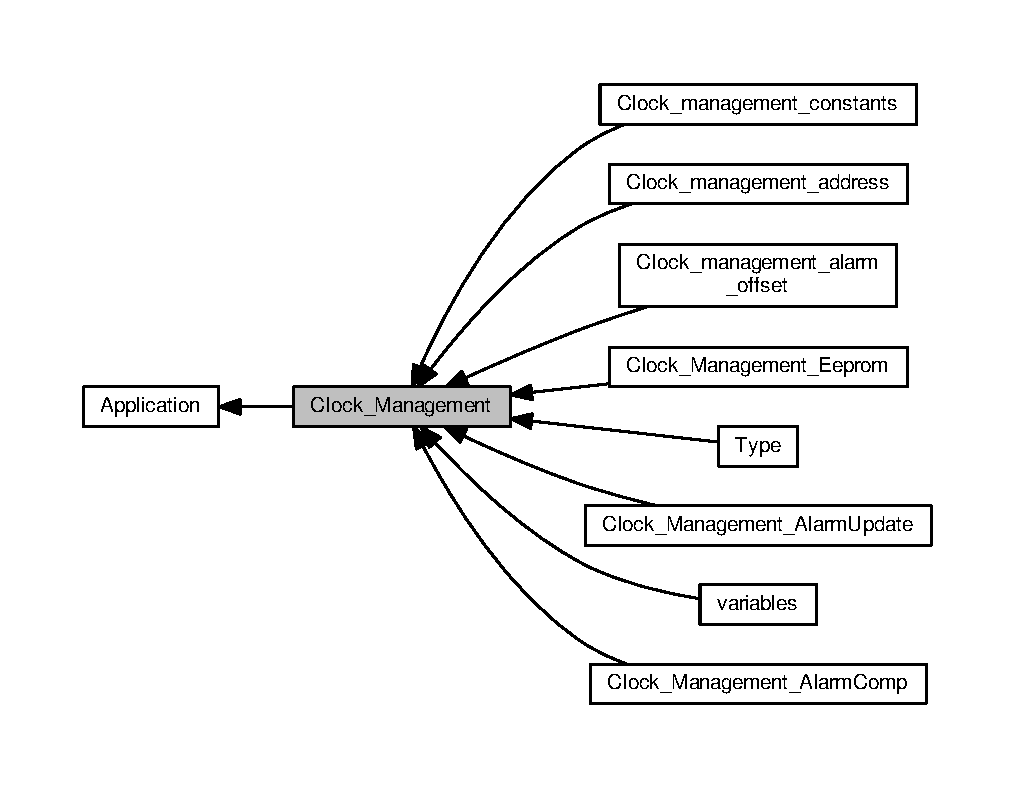
\includegraphics[width=350pt]{d5/d84/group___clock___management}
\end{center}
\end{figure}
\subsection*{Modules}
\begin{DoxyCompactItemize}
\item 
\hyperlink{group___clock__management__address}{Clock\+\_\+management\+\_\+address}
\item 
\hyperlink{group___clock__management__alarm__offset}{Clock\+\_\+management\+\_\+alarm\+\_\+offset}
\item 
\hyperlink{group___clock__management__constants}{Clock\+\_\+management\+\_\+constants}
\item 
\hyperlink{group__clock__management}{variables}
\item 
\hyperlink{group__type}{Type}
\begin{DoxyCompactList}\small\item\em Alarm type. \end{DoxyCompactList}\item 
\hyperlink{group___clock___management___eeprom}{Clock\+\_\+\+Management\+\_\+\+Eeprom}
\begin{DoxyCompactList}\small\item\em Saving and Loading of clock information. \end{DoxyCompactList}\item 
\hyperlink{group___clock___management___alarm_comp}{Clock\+\_\+\+Management\+\_\+\+Alarm\+Comp}
\begin{DoxyCompactList}\small\item\em Comparison between dates, times and alarms. \end{DoxyCompactList}\item 
\hyperlink{group___clock___management___alarm_update}{Clock\+\_\+\+Management\+\_\+\+Alarm\+Update}
\begin{DoxyCompactList}\small\item\em Manages updates of alarms and alarm parameters. \end{DoxyCompactList}\end{DoxyCompactItemize}


\subsection{Detailed Description}

\hypertarget{group___constant}{}\section{Constant}
\label{group___constant}\index{Constant@{Constant}}


Define audio frequency and D\+MA frequency.  


\subsection*{Macros}
\begin{DoxyCompactItemize}
\item 
\mbox{\Hypertarget{group___constant_gaae969438a57a86fddf0cf53106c9b6b4}\label{group___constant_gaae969438a57a86fddf0cf53106c9b6b4}} 
\#define {\bfseries A\+U\+D\+I\+O\+\_\+\+F\+R\+E\+Q\+U\+E\+N\+CY}~11000
\item 
\mbox{\Hypertarget{group___constant_ga644d7863b10926e5fb77205f294e1964}\label{group___constant_ga644d7863b10926e5fb77205f294e1964}} 
\#define {\bfseries D\+M\+A\+\_\+\+F\+R\+E\+Q\+U\+E\+N\+CY}~(86000000/(2$\ast$A\+U\+D\+I\+O\+\_\+\+F\+R\+E\+Q\+U\+E\+N\+CY))
\item 
\mbox{\Hypertarget{group___constant_ga857df980c46f31dbe009560d826413a8}\label{group___constant_ga857df980c46f31dbe009560d826413a8}} 
\#define {\bfseries W\+S2812\+\_\+\+F\+R\+EQ}~(8\+E5)
\item 
\mbox{\Hypertarget{group___constant_ga5f1fac9f0aaabad0683c04e44a1aefe9}\label{group___constant_ga5f1fac9f0aaabad0683c04e44a1aefe9}} 
\#define {\bfseries T\+I\+M\+E\+R\+\_\+\+C\+L\+O\+C\+K\+\_\+\+F\+R\+EQ}~(84\+E6)
\item 
\mbox{\Hypertarget{group___constant_gad888acf7c13a4bedd6541ceb5cf9bf6d}\label{group___constant_gad888acf7c13a4bedd6541ceb5cf9bf6d}} 
\#define {\bfseries T\+I\+M\+E\+R\+\_\+\+P\+E\+R\+I\+OD}~(T\+I\+M\+E\+R\+\_\+\+C\+L\+O\+C\+K\+\_\+\+F\+R\+EQ / W\+S2812\+\_\+\+F\+R\+EQ)
\item 
\mbox{\Hypertarget{group___constant_ga306db1a2fccc9c26ad114b50a88940d3}\label{group___constant_ga306db1a2fccc9c26ad114b50a88940d3}} 
\#define {\bfseries L\+E\+D\+\_\+\+N\+U\+M\+B\+ER}~(4)
\item 
\mbox{\Hypertarget{group___constant_ga7af472c9efcf021651c589bb54d103fa}\label{group___constant_ga7af472c9efcf021651c589bb54d103fa}} 
\#define {\bfseries L\+E\+D\+\_\+\+D\+A\+T\+A\+\_\+\+S\+I\+ZE}~(L\+E\+D\+\_\+\+N\+U\+M\+B\+ER $\ast$ 24)
\item 
\mbox{\Hypertarget{group___constant_ga38b56d14857b32e86b876a32957a2b63}\label{group___constant_ga38b56d14857b32e86b876a32957a2b63}} 
\#define {\bfseries R\+E\+S\+E\+T\+\_\+\+S\+L\+O\+T\+S\+\_\+\+B\+E\+G\+IN}~(50)
\item 
\mbox{\Hypertarget{group___constant_ga91e46b7f75ff75a4719a9d7f589df5a3}\label{group___constant_ga91e46b7f75ff75a4719a9d7f589df5a3}} 
\#define {\bfseries R\+E\+S\+E\+T\+\_\+\+S\+L\+O\+T\+S\+\_\+\+E\+ND}~(50)
\item 
\mbox{\Hypertarget{group___constant_gacbccf04b27120fd8ba0a8eae7866291f}\label{group___constant_gacbccf04b27120fd8ba0a8eae7866291f}} 
\#define {\bfseries W\+S2812\+\_\+\+L\+A\+S\+T\+\_\+\+S\+L\+OT}~(1)
\item 
\mbox{\Hypertarget{group___constant_ga398165d967d8a2c8ff57ddd0a081a5ff}\label{group___constant_ga398165d967d8a2c8ff57ddd0a081a5ff}} 
\#define {\bfseries L\+E\+D\+\_\+\+B\+U\+F\+F\+E\+R\+\_\+\+S\+I\+ZE}~(R\+E\+S\+E\+T\+\_\+\+S\+L\+O\+T\+S\+\_\+\+B\+E\+G\+IN + L\+E\+D\+\_\+\+D\+A\+T\+A\+\_\+\+S\+I\+ZE + W\+S2812\+\_\+\+L\+A\+S\+T\+\_\+\+S\+L\+OT + R\+E\+S\+E\+T\+\_\+\+S\+L\+O\+T\+S\+\_\+\+E\+ND)
\item 
\mbox{\Hypertarget{group___constant_ga3c67cd1a76ba7e85676da5f023f42430}\label{group___constant_ga3c67cd1a76ba7e85676da5f023f42430}} 
\#define {\bfseries W\+S2812\+\_\+0}~(T\+I\+M\+E\+R\+\_\+\+P\+E\+R\+I\+OD / 3)
\item 
\mbox{\Hypertarget{group___constant_gad4cec7bff3f072ffe9ec1e11324c7418}\label{group___constant_gad4cec7bff3f072ffe9ec1e11324c7418}} 
\#define {\bfseries W\+S2812\+\_\+1}~(T\+I\+M\+E\+R\+\_\+\+P\+E\+R\+I\+OD $\ast$ 2 / 3)
\item 
\mbox{\Hypertarget{group___constant_gaef8a90792d52a7085de6c0affec15557}\label{group___constant_gaef8a90792d52a7085de6c0affec15557}} 
\#define {\bfseries W\+S2812\+\_\+\+R\+E\+S\+ET}~(0)
\item 
\mbox{\Hypertarget{group___constant_gaaf645a2813f2274619a70855afb92aca}\label{group___constant_gaaf645a2813f2274619a70855afb92aca}} 
\#define {\bfseries M\+A\+X\+\_\+8\+B\+IT}~(255)
\end{DoxyCompactItemize}


\subsection{Detailed Description}
Define audio frequency and D\+MA frequency. 

Defines constants.
\hypertarget{group___audio___init}{}\section{Configuration functions}
\label{group___audio___init}\index{Configuration functions@{Configuration functions}}


Audio configuration functions.  


Collaboration diagram for Configuration functions\+:\nopagebreak
\begin{figure}[H]
\begin{center}
\leavevmode
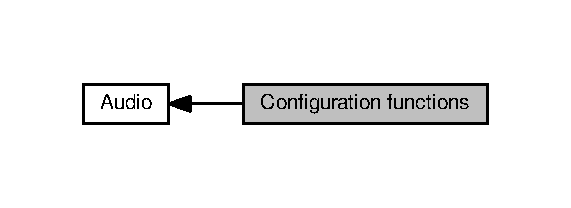
\includegraphics[width=274pt]{d0/df3/group___audio___init}
\end{center}
\end{figure}
\subsection*{Functions}
\begin{DoxyCompactItemize}
\item 
void \hyperlink{group___audio___init_gafff6cd7f4332d078ce0114143cd30998}{audio\+\_\+disable} (void)
\begin{DoxyCompactList}\small\item\em Disable the D\+MA. \end{DoxyCompactList}\item 
void \hyperlink{group___audio___init_gabcda20e7d4baa315d151230fcc81ec1d}{audio\+\_\+init} (uint16\+\_\+t $\ast$D\+A\+C\+Buffer, uint16\+\_\+t Size)
\begin{DoxyCompactList}\small\item\em Perform audio initialization. \end{DoxyCompactList}\end{DoxyCompactItemize}


\subsection{Detailed Description}
Audio configuration functions. 



\subsection{Function Documentation}
\index{Configuration functions@{Configuration functions}!audio\+\_\+disable@{audio\+\_\+disable}}
\index{audio\+\_\+disable@{audio\+\_\+disable}!Configuration functions@{Configuration functions}}
\subsubsection[{\texorpdfstring{audio\+\_\+disable(void)}{audio_disable(void)}}]{\setlength{\rightskip}{0pt plus 5cm}void audio\+\_\+disable (
\begin{DoxyParamCaption}
\item[{void}]{}
\end{DoxyParamCaption}
)}\hypertarget{group___audio___init_gafff6cd7f4332d078ce0114143cd30998}{}\label{group___audio___init_gafff6cd7f4332d078ce0114143cd30998}


Disable the D\+MA. 


\begin{DoxyParams}{Parameters}
{\em None} & \\
\hline
\end{DoxyParams}

\begin{DoxyRetVals}{Return values}
{\em None} & \\
\hline
\end{DoxyRetVals}


Definition at line 48 of file N\+P\+C\+\_\+audio.\+c.



Here is the caller graph for this function\+:\nopagebreak
\begin{figure}[H]
\begin{center}
\leavevmode
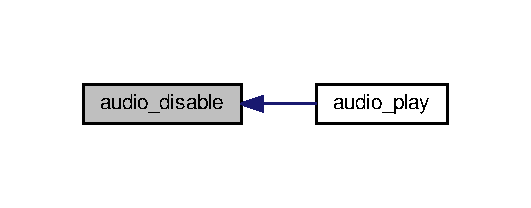
\includegraphics[width=255pt]{d0/df3/group___audio___init_gafff6cd7f4332d078ce0114143cd30998_icgraph}
\end{center}
\end{figure}


\index{Configuration functions@{Configuration functions}!audio\+\_\+init@{audio\+\_\+init}}
\index{audio\+\_\+init@{audio\+\_\+init}!Configuration functions@{Configuration functions}}
\subsubsection[{\texorpdfstring{audio\+\_\+init(uint16\+\_\+t $\ast$\+D\+A\+C\+Buffer, uint16\+\_\+t Size)}{audio_init(uint16_t *DACBuffer, uint16_t Size)}}]{\setlength{\rightskip}{0pt plus 5cm}void audio\+\_\+init (
\begin{DoxyParamCaption}
\item[{uint16\+\_\+t $\ast$}]{D\+A\+C\+Buffer, }
\item[{uint16\+\_\+t}]{Size}
\end{DoxyParamCaption}
)}\hypertarget{group___audio___init_gabcda20e7d4baa315d151230fcc81ec1d}{}\label{group___audio___init_gabcda20e7d4baa315d151230fcc81ec1d}


Perform audio initialization. 


\begin{DoxyParams}{Parameters}
{\em D\+A\+C\+Buffer} & Array to be pushed to the D\+MA \\
\hline
{\em Mode} & D\+MA Mode (default\+:D\+M\+A\+\_\+\+Mode\+\_\+\+Normal) \\
\hline
{\em Size} & sample size (default\+:S\+A\+M\+P\+L\+E\+\_\+\+S\+I\+ZE) \\
\hline
\end{DoxyParams}

\begin{DoxyRetVals}{Return values}
{\em None} & \\
\hline
\end{DoxyRetVals}


Definition at line 61 of file N\+P\+C\+\_\+audio.\+c.



Here is the caller graph for this function\+:\nopagebreak
\begin{figure}[H]
\begin{center}
\leavevmode
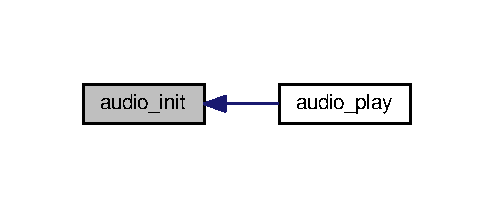
\includegraphics[width=237pt]{d0/df3/group___audio___init_gabcda20e7d4baa315d151230fcc81ec1d_icgraph}
\end{center}
\end{figure}



\hypertarget{group___audio___play}{}\section{Play audio functions}
\label{group___audio___play}\index{Play audio functions@{Play audio functions}}


Audio functions.  


Collaboration diagram for Play audio functions\+:\nopagebreak
\begin{figure}[H]
\begin{center}
\leavevmode
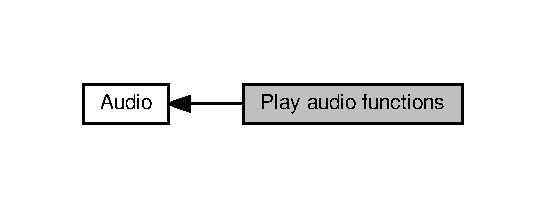
\includegraphics[width=262pt]{de/d72/group___audio___play}
\end{center}
\end{figure}
\subsection*{Functions}
\begin{DoxyCompactItemize}
\item 
void \hyperlink{group___audio___play_gaf73a37418a80bbb39f75abe8b60b0afb}{audio\+\_\+play} (uint16\+\_\+t $\ast$D\+A\+C\+Buffer, uint16\+\_\+t Size)
\begin{DoxyCompactList}\small\item\em Play a sample. \end{DoxyCompactList}\end{DoxyCompactItemize}


\subsection{Detailed Description}
Audio functions. 



\subsection{Function Documentation}
\index{Play audio functions@{Play audio functions}!audio\+\_\+play@{audio\+\_\+play}}
\index{audio\+\_\+play@{audio\+\_\+play}!Play audio functions@{Play audio functions}}
\subsubsection[{\texorpdfstring{audio\+\_\+play(uint16\+\_\+t $\ast$\+D\+A\+C\+Buffer, uint16\+\_\+t Size)}{audio_play(uint16_t *DACBuffer, uint16_t Size)}}]{\setlength{\rightskip}{0pt plus 5cm}void audio\+\_\+play (
\begin{DoxyParamCaption}
\item[{uint16\+\_\+t $\ast$}]{D\+A\+C\+Buffer, }
\item[{uint16\+\_\+t}]{Size}
\end{DoxyParamCaption}
)}\hypertarget{group___audio___play_gaf73a37418a80bbb39f75abe8b60b0afb}{}\label{group___audio___play_gaf73a37418a80bbb39f75abe8b60b0afb}


Play a sample. 


\begin{DoxyParams}{Parameters}
{\em D\+A\+C\+Buffer} & Array to be pushed to the D\+MA \\
\hline
{\em Size} & sample size (default\+:S\+A\+M\+P\+L\+E\+\_\+\+S\+I\+ZE) \\
\hline
\end{DoxyParams}
\begin{DoxyReturn}{Returns}
None 
\end{DoxyReturn}


Definition at line 136 of file N\+P\+C\+\_\+audio.\+c.



Here is the call graph for this function\+:\nopagebreak
\begin{figure}[H]
\begin{center}
\leavevmode
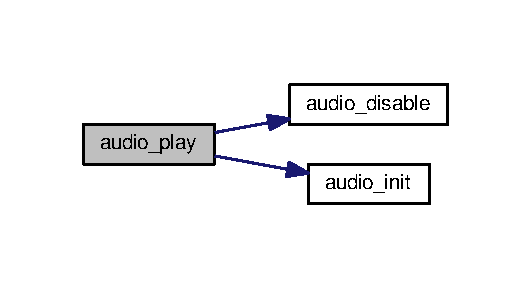
\includegraphics[width=255pt]{de/d72/group___audio___play_gaf73a37418a80bbb39f75abe8b60b0afb_cgraph}
\end{center}
\end{figure}



\hypertarget{group__bluetooth___constants}{}\section{Bluetooth\+\_\+\+Constants}
\label{group__bluetooth___constants}\index{Bluetooth\+\_\+\+Constants@{Bluetooth\+\_\+\+Constants}}


define bluetooth constant  


Collaboration diagram for Bluetooth\+\_\+\+Constants\+:\nopagebreak
\begin{figure}[H]
\begin{center}
\leavevmode
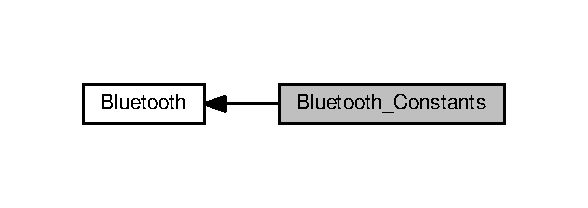
\includegraphics[width=282pt]{d2/d60/group__bluetooth___constants}
\end{center}
\end{figure}
\subsection*{Macros}
\begin{DoxyCompactItemize}
\item 
\#define \hyperlink{group__bluetooth___constants_gac4b97204cfdd1ad5faebd0a56a6521c6}{B\+L\+U\+E\+T\+O\+O\+T\+H\+\_\+\+P\+E\+R\+I\+P\+H\+\_\+\+U\+S\+A\+R\+TX}~R\+C\+C\+\_\+\+A\+P\+B2\+Periph\+\_\+\+U\+S\+A\+R\+T1
\item 
\#define \hyperlink{group__bluetooth___constants_gab9bf1b33e271246e795a3847516e0949}{B\+L\+U\+E\+T\+O\+O\+T\+H\+\_\+\+P\+E\+R\+I\+P\+H\+\_\+\+G\+P\+I\+OX}~R\+C\+C\+\_\+\+A\+H\+B1\+Periph\+\_\+\+G\+P\+I\+OB
\item 
\#define \hyperlink{group__bluetooth___constants_gad47fcf58a7d55e48e039420b36350fcd}{B\+L\+U\+E\+T\+O\+O\+T\+H\+\_\+\+G\+P\+I\+OX}~G\+P\+I\+OB
\item 
\#define \hyperlink{group__bluetooth___constants_ga03828dc38b1dd4e24867280ccaf54c1e}{B\+L\+U\+E\+T\+O\+O\+T\+H\+\_\+\+T\+X\+\_\+\+P\+IN}~G\+P\+I\+O\+\_\+\+Pin\+\_\+6
\item 
\#define \hyperlink{group__bluetooth___constants_gad6b845bce7449baa7ebc4f2625c32165}{B\+L\+U\+E\+T\+O\+O\+T\+H\+\_\+\+R\+X\+\_\+\+P\+IN}~G\+P\+I\+O\+\_\+\+Pin\+\_\+7
\item 
\#define \hyperlink{group__bluetooth___constants_gaae23de9ae44f36e0a519e010e545d579}{B\+L\+U\+E\+T\+O\+O\+T\+H\+\_\+\+T\+X\+\_\+\+P\+I\+N\+S\+O\+U\+R\+CE}~G\+P\+I\+O\+\_\+\+Pin\+Source6
\item 
\#define \hyperlink{group__bluetooth___constants_gaf8abe33a7c3b953bc50789da61176ce8}{B\+L\+U\+E\+T\+O\+O\+T\+H\+\_\+\+R\+X\+\_\+\+P\+I\+N\+S\+O\+U\+R\+CE}~G\+P\+I\+O\+\_\+\+Pin\+Source7
\item 
\#define \hyperlink{group__bluetooth___constants_ga89cad714e99e26757fe9208e98c6cbe9}{B\+L\+U\+E\+T\+O\+O\+T\+H\+\_\+\+A\+F\+\_\+\+U\+S\+A\+RT}~G\+P\+I\+O\+\_\+\+A\+F\+\_\+\+U\+S\+A\+R\+T1
\item 
\#define \hyperlink{group__bluetooth___constants_gac9aff5be09be7a2e3c84d99794f80dc3}{B\+L\+U\+E\+T\+O\+O\+T\+H\+\_\+\+U\+S\+A\+R\+TX}~U\+S\+A\+R\+T1
\item 
\#define \hyperlink{group__bluetooth___constants_ga6049290b6a001e8af7bc24ebe06f8ee8}{B\+L\+U\+E\+T\+O\+O\+T\+H\+\_\+\+U\+S\+A\+R\+T\+X\+\_\+\+I\+RQ}~U\+S\+A\+R\+T1\+\_\+\+I\+R\+Qn
\item 
\#define \hyperlink{group__bluetooth___constants_ga800ec9bb77245339c6a2b770432e0232}{B\+L\+U\+E\+T\+O\+O\+T\+H\+\_\+\+B\+A\+U\+D\+R\+A\+TE}~9600
\end{DoxyCompactItemize}


\subsection{Detailed Description}
define bluetooth constant 



\subsection{Macro Definition Documentation}
\index{Bluetooth\+\_\+\+Constants@{Bluetooth\+\_\+\+Constants}!B\+L\+U\+E\+T\+O\+O\+T\+H\+\_\+\+A\+F\+\_\+\+U\+S\+A\+RT@{B\+L\+U\+E\+T\+O\+O\+T\+H\+\_\+\+A\+F\+\_\+\+U\+S\+A\+RT}}
\index{B\+L\+U\+E\+T\+O\+O\+T\+H\+\_\+\+A\+F\+\_\+\+U\+S\+A\+RT@{B\+L\+U\+E\+T\+O\+O\+T\+H\+\_\+\+A\+F\+\_\+\+U\+S\+A\+RT}!Bluetooth\+\_\+\+Constants@{Bluetooth\+\_\+\+Constants}}
\subsubsection[{\texorpdfstring{B\+L\+U\+E\+T\+O\+O\+T\+H\+\_\+\+A\+F\+\_\+\+U\+S\+A\+RT}{BLUETOOTH_AF_USART}}]{\setlength{\rightskip}{0pt plus 5cm}\#define B\+L\+U\+E\+T\+O\+O\+T\+H\+\_\+\+A\+F\+\_\+\+U\+S\+A\+RT~G\+P\+I\+O\+\_\+\+A\+F\+\_\+\+U\+S\+A\+R\+T1}\hypertarget{group__bluetooth___constants_ga89cad714e99e26757fe9208e98c6cbe9}{}\label{group__bluetooth___constants_ga89cad714e99e26757fe9208e98c6cbe9}


Definition at line 48 of file N\+P\+C\+\_\+bluetooth.\+h.

\index{Bluetooth\+\_\+\+Constants@{Bluetooth\+\_\+\+Constants}!B\+L\+U\+E\+T\+O\+O\+T\+H\+\_\+\+B\+A\+U\+D\+R\+A\+TE@{B\+L\+U\+E\+T\+O\+O\+T\+H\+\_\+\+B\+A\+U\+D\+R\+A\+TE}}
\index{B\+L\+U\+E\+T\+O\+O\+T\+H\+\_\+\+B\+A\+U\+D\+R\+A\+TE@{B\+L\+U\+E\+T\+O\+O\+T\+H\+\_\+\+B\+A\+U\+D\+R\+A\+TE}!Bluetooth\+\_\+\+Constants@{Bluetooth\+\_\+\+Constants}}
\subsubsection[{\texorpdfstring{B\+L\+U\+E\+T\+O\+O\+T\+H\+\_\+\+B\+A\+U\+D\+R\+A\+TE}{BLUETOOTH_BAUDRATE}}]{\setlength{\rightskip}{0pt plus 5cm}\#define B\+L\+U\+E\+T\+O\+O\+T\+H\+\_\+\+B\+A\+U\+D\+R\+A\+TE~9600}\hypertarget{group__bluetooth___constants_ga800ec9bb77245339c6a2b770432e0232}{}\label{group__bluetooth___constants_ga800ec9bb77245339c6a2b770432e0232}


Definition at line 51 of file N\+P\+C\+\_\+bluetooth.\+h.

\index{Bluetooth\+\_\+\+Constants@{Bluetooth\+\_\+\+Constants}!B\+L\+U\+E\+T\+O\+O\+T\+H\+\_\+\+G\+P\+I\+OX@{B\+L\+U\+E\+T\+O\+O\+T\+H\+\_\+\+G\+P\+I\+OX}}
\index{B\+L\+U\+E\+T\+O\+O\+T\+H\+\_\+\+G\+P\+I\+OX@{B\+L\+U\+E\+T\+O\+O\+T\+H\+\_\+\+G\+P\+I\+OX}!Bluetooth\+\_\+\+Constants@{Bluetooth\+\_\+\+Constants}}
\subsubsection[{\texorpdfstring{B\+L\+U\+E\+T\+O\+O\+T\+H\+\_\+\+G\+P\+I\+OX}{BLUETOOTH_GPIOX}}]{\setlength{\rightskip}{0pt plus 5cm}\#define B\+L\+U\+E\+T\+O\+O\+T\+H\+\_\+\+G\+P\+I\+OX~G\+P\+I\+OB}\hypertarget{group__bluetooth___constants_gad47fcf58a7d55e48e039420b36350fcd}{}\label{group__bluetooth___constants_gad47fcf58a7d55e48e039420b36350fcd}


Definition at line 43 of file N\+P\+C\+\_\+bluetooth.\+h.

\index{Bluetooth\+\_\+\+Constants@{Bluetooth\+\_\+\+Constants}!B\+L\+U\+E\+T\+O\+O\+T\+H\+\_\+\+P\+E\+R\+I\+P\+H\+\_\+\+G\+P\+I\+OX@{B\+L\+U\+E\+T\+O\+O\+T\+H\+\_\+\+P\+E\+R\+I\+P\+H\+\_\+\+G\+P\+I\+OX}}
\index{B\+L\+U\+E\+T\+O\+O\+T\+H\+\_\+\+P\+E\+R\+I\+P\+H\+\_\+\+G\+P\+I\+OX@{B\+L\+U\+E\+T\+O\+O\+T\+H\+\_\+\+P\+E\+R\+I\+P\+H\+\_\+\+G\+P\+I\+OX}!Bluetooth\+\_\+\+Constants@{Bluetooth\+\_\+\+Constants}}
\subsubsection[{\texorpdfstring{B\+L\+U\+E\+T\+O\+O\+T\+H\+\_\+\+P\+E\+R\+I\+P\+H\+\_\+\+G\+P\+I\+OX}{BLUETOOTH_PERIPH_GPIOX}}]{\setlength{\rightskip}{0pt plus 5cm}\#define B\+L\+U\+E\+T\+O\+O\+T\+H\+\_\+\+P\+E\+R\+I\+P\+H\+\_\+\+G\+P\+I\+OX~R\+C\+C\+\_\+\+A\+H\+B1\+Periph\+\_\+\+G\+P\+I\+OB}\hypertarget{group__bluetooth___constants_gab9bf1b33e271246e795a3847516e0949}{}\label{group__bluetooth___constants_gab9bf1b33e271246e795a3847516e0949}


Definition at line 42 of file N\+P\+C\+\_\+bluetooth.\+h.

\index{Bluetooth\+\_\+\+Constants@{Bluetooth\+\_\+\+Constants}!B\+L\+U\+E\+T\+O\+O\+T\+H\+\_\+\+P\+E\+R\+I\+P\+H\+\_\+\+U\+S\+A\+R\+TX@{B\+L\+U\+E\+T\+O\+O\+T\+H\+\_\+\+P\+E\+R\+I\+P\+H\+\_\+\+U\+S\+A\+R\+TX}}
\index{B\+L\+U\+E\+T\+O\+O\+T\+H\+\_\+\+P\+E\+R\+I\+P\+H\+\_\+\+U\+S\+A\+R\+TX@{B\+L\+U\+E\+T\+O\+O\+T\+H\+\_\+\+P\+E\+R\+I\+P\+H\+\_\+\+U\+S\+A\+R\+TX}!Bluetooth\+\_\+\+Constants@{Bluetooth\+\_\+\+Constants}}
\subsubsection[{\texorpdfstring{B\+L\+U\+E\+T\+O\+O\+T\+H\+\_\+\+P\+E\+R\+I\+P\+H\+\_\+\+U\+S\+A\+R\+TX}{BLUETOOTH_PERIPH_USARTX}}]{\setlength{\rightskip}{0pt plus 5cm}\#define B\+L\+U\+E\+T\+O\+O\+T\+H\+\_\+\+P\+E\+R\+I\+P\+H\+\_\+\+U\+S\+A\+R\+TX~R\+C\+C\+\_\+\+A\+P\+B2\+Periph\+\_\+\+U\+S\+A\+R\+T1}\hypertarget{group__bluetooth___constants_gac4b97204cfdd1ad5faebd0a56a6521c6}{}\label{group__bluetooth___constants_gac4b97204cfdd1ad5faebd0a56a6521c6}


Definition at line 41 of file N\+P\+C\+\_\+bluetooth.\+h.

\index{Bluetooth\+\_\+\+Constants@{Bluetooth\+\_\+\+Constants}!B\+L\+U\+E\+T\+O\+O\+T\+H\+\_\+\+R\+X\+\_\+\+P\+IN@{B\+L\+U\+E\+T\+O\+O\+T\+H\+\_\+\+R\+X\+\_\+\+P\+IN}}
\index{B\+L\+U\+E\+T\+O\+O\+T\+H\+\_\+\+R\+X\+\_\+\+P\+IN@{B\+L\+U\+E\+T\+O\+O\+T\+H\+\_\+\+R\+X\+\_\+\+P\+IN}!Bluetooth\+\_\+\+Constants@{Bluetooth\+\_\+\+Constants}}
\subsubsection[{\texorpdfstring{B\+L\+U\+E\+T\+O\+O\+T\+H\+\_\+\+R\+X\+\_\+\+P\+IN}{BLUETOOTH_RX_PIN}}]{\setlength{\rightskip}{0pt plus 5cm}\#define B\+L\+U\+E\+T\+O\+O\+T\+H\+\_\+\+R\+X\+\_\+\+P\+IN~G\+P\+I\+O\+\_\+\+Pin\+\_\+7}\hypertarget{group__bluetooth___constants_gad6b845bce7449baa7ebc4f2625c32165}{}\label{group__bluetooth___constants_gad6b845bce7449baa7ebc4f2625c32165}


Definition at line 45 of file N\+P\+C\+\_\+bluetooth.\+h.

\index{Bluetooth\+\_\+\+Constants@{Bluetooth\+\_\+\+Constants}!B\+L\+U\+E\+T\+O\+O\+T\+H\+\_\+\+R\+X\+\_\+\+P\+I\+N\+S\+O\+U\+R\+CE@{B\+L\+U\+E\+T\+O\+O\+T\+H\+\_\+\+R\+X\+\_\+\+P\+I\+N\+S\+O\+U\+R\+CE}}
\index{B\+L\+U\+E\+T\+O\+O\+T\+H\+\_\+\+R\+X\+\_\+\+P\+I\+N\+S\+O\+U\+R\+CE@{B\+L\+U\+E\+T\+O\+O\+T\+H\+\_\+\+R\+X\+\_\+\+P\+I\+N\+S\+O\+U\+R\+CE}!Bluetooth\+\_\+\+Constants@{Bluetooth\+\_\+\+Constants}}
\subsubsection[{\texorpdfstring{B\+L\+U\+E\+T\+O\+O\+T\+H\+\_\+\+R\+X\+\_\+\+P\+I\+N\+S\+O\+U\+R\+CE}{BLUETOOTH_RX_PINSOURCE}}]{\setlength{\rightskip}{0pt plus 5cm}\#define B\+L\+U\+E\+T\+O\+O\+T\+H\+\_\+\+R\+X\+\_\+\+P\+I\+N\+S\+O\+U\+R\+CE~G\+P\+I\+O\+\_\+\+Pin\+Source7}\hypertarget{group__bluetooth___constants_gaf8abe33a7c3b953bc50789da61176ce8}{}\label{group__bluetooth___constants_gaf8abe33a7c3b953bc50789da61176ce8}


Definition at line 47 of file N\+P\+C\+\_\+bluetooth.\+h.

\index{Bluetooth\+\_\+\+Constants@{Bluetooth\+\_\+\+Constants}!B\+L\+U\+E\+T\+O\+O\+T\+H\+\_\+\+T\+X\+\_\+\+P\+IN@{B\+L\+U\+E\+T\+O\+O\+T\+H\+\_\+\+T\+X\+\_\+\+P\+IN}}
\index{B\+L\+U\+E\+T\+O\+O\+T\+H\+\_\+\+T\+X\+\_\+\+P\+IN@{B\+L\+U\+E\+T\+O\+O\+T\+H\+\_\+\+T\+X\+\_\+\+P\+IN}!Bluetooth\+\_\+\+Constants@{Bluetooth\+\_\+\+Constants}}
\subsubsection[{\texorpdfstring{B\+L\+U\+E\+T\+O\+O\+T\+H\+\_\+\+T\+X\+\_\+\+P\+IN}{BLUETOOTH_TX_PIN}}]{\setlength{\rightskip}{0pt plus 5cm}\#define B\+L\+U\+E\+T\+O\+O\+T\+H\+\_\+\+T\+X\+\_\+\+P\+IN~G\+P\+I\+O\+\_\+\+Pin\+\_\+6}\hypertarget{group__bluetooth___constants_ga03828dc38b1dd4e24867280ccaf54c1e}{}\label{group__bluetooth___constants_ga03828dc38b1dd4e24867280ccaf54c1e}


Definition at line 44 of file N\+P\+C\+\_\+bluetooth.\+h.

\index{Bluetooth\+\_\+\+Constants@{Bluetooth\+\_\+\+Constants}!B\+L\+U\+E\+T\+O\+O\+T\+H\+\_\+\+T\+X\+\_\+\+P\+I\+N\+S\+O\+U\+R\+CE@{B\+L\+U\+E\+T\+O\+O\+T\+H\+\_\+\+T\+X\+\_\+\+P\+I\+N\+S\+O\+U\+R\+CE}}
\index{B\+L\+U\+E\+T\+O\+O\+T\+H\+\_\+\+T\+X\+\_\+\+P\+I\+N\+S\+O\+U\+R\+CE@{B\+L\+U\+E\+T\+O\+O\+T\+H\+\_\+\+T\+X\+\_\+\+P\+I\+N\+S\+O\+U\+R\+CE}!Bluetooth\+\_\+\+Constants@{Bluetooth\+\_\+\+Constants}}
\subsubsection[{\texorpdfstring{B\+L\+U\+E\+T\+O\+O\+T\+H\+\_\+\+T\+X\+\_\+\+P\+I\+N\+S\+O\+U\+R\+CE}{BLUETOOTH_TX_PINSOURCE}}]{\setlength{\rightskip}{0pt plus 5cm}\#define B\+L\+U\+E\+T\+O\+O\+T\+H\+\_\+\+T\+X\+\_\+\+P\+I\+N\+S\+O\+U\+R\+CE~G\+P\+I\+O\+\_\+\+Pin\+Source6}\hypertarget{group__bluetooth___constants_gaae23de9ae44f36e0a519e010e545d579}{}\label{group__bluetooth___constants_gaae23de9ae44f36e0a519e010e545d579}


Definition at line 46 of file N\+P\+C\+\_\+bluetooth.\+h.

\index{Bluetooth\+\_\+\+Constants@{Bluetooth\+\_\+\+Constants}!B\+L\+U\+E\+T\+O\+O\+T\+H\+\_\+\+U\+S\+A\+R\+TX@{B\+L\+U\+E\+T\+O\+O\+T\+H\+\_\+\+U\+S\+A\+R\+TX}}
\index{B\+L\+U\+E\+T\+O\+O\+T\+H\+\_\+\+U\+S\+A\+R\+TX@{B\+L\+U\+E\+T\+O\+O\+T\+H\+\_\+\+U\+S\+A\+R\+TX}!Bluetooth\+\_\+\+Constants@{Bluetooth\+\_\+\+Constants}}
\subsubsection[{\texorpdfstring{B\+L\+U\+E\+T\+O\+O\+T\+H\+\_\+\+U\+S\+A\+R\+TX}{BLUETOOTH_USARTX}}]{\setlength{\rightskip}{0pt plus 5cm}\#define B\+L\+U\+E\+T\+O\+O\+T\+H\+\_\+\+U\+S\+A\+R\+TX~U\+S\+A\+R\+T1}\hypertarget{group__bluetooth___constants_gac9aff5be09be7a2e3c84d99794f80dc3}{}\label{group__bluetooth___constants_gac9aff5be09be7a2e3c84d99794f80dc3}


Definition at line 49 of file N\+P\+C\+\_\+bluetooth.\+h.

\index{Bluetooth\+\_\+\+Constants@{Bluetooth\+\_\+\+Constants}!B\+L\+U\+E\+T\+O\+O\+T\+H\+\_\+\+U\+S\+A\+R\+T\+X\+\_\+\+I\+RQ@{B\+L\+U\+E\+T\+O\+O\+T\+H\+\_\+\+U\+S\+A\+R\+T\+X\+\_\+\+I\+RQ}}
\index{B\+L\+U\+E\+T\+O\+O\+T\+H\+\_\+\+U\+S\+A\+R\+T\+X\+\_\+\+I\+RQ@{B\+L\+U\+E\+T\+O\+O\+T\+H\+\_\+\+U\+S\+A\+R\+T\+X\+\_\+\+I\+RQ}!Bluetooth\+\_\+\+Constants@{Bluetooth\+\_\+\+Constants}}
\subsubsection[{\texorpdfstring{B\+L\+U\+E\+T\+O\+O\+T\+H\+\_\+\+U\+S\+A\+R\+T\+X\+\_\+\+I\+RQ}{BLUETOOTH_USARTX_IRQ}}]{\setlength{\rightskip}{0pt plus 5cm}\#define B\+L\+U\+E\+T\+O\+O\+T\+H\+\_\+\+U\+S\+A\+R\+T\+X\+\_\+\+I\+RQ~U\+S\+A\+R\+T1\+\_\+\+I\+R\+Qn}\hypertarget{group__bluetooth___constants_ga6049290b6a001e8af7bc24ebe06f8ee8}{}\label{group__bluetooth___constants_ga6049290b6a001e8af7bc24ebe06f8ee8}


Definition at line 50 of file N\+P\+C\+\_\+bluetooth.\+h.


\hypertarget{group__bluetooth___init}{}\section{Initialization and transmission handler functions}
\label{group__bluetooth___init}\index{Initialization and transmission handler functions@{Initialization and transmission handler functions}}


bluetooth initialization functions  


Collaboration diagram for Initialization and transmission handler functions\+:\nopagebreak
\begin{figure}[H]
\begin{center}
\leavevmode
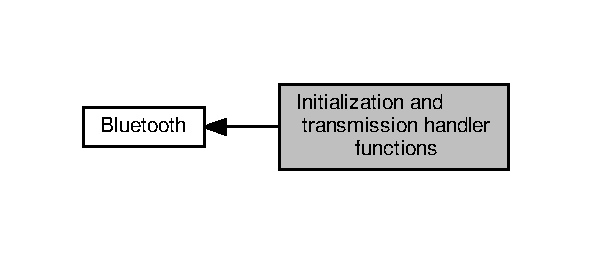
\includegraphics[width=284pt]{d7/d87/group__bluetooth___init}
\end{center}
\end{figure}
\subsection*{Functions}
\begin{DoxyCompactItemize}
\item 
void \hyperlink{group__bluetooth___init_gaaa60810e0857e9e1e5b2cba80b8db3ff}{bluetooth\+\_\+init} (void)
\begin{DoxyCompactList}\small\item\em Initialize the bluetooth and set baudrate to 9600. \end{DoxyCompactList}\item 
void \hyperlink{group__bluetooth___init_ga7139cd4baabbbcbab0c1fe6d7d4ae1cc}{U\+S\+A\+R\+T1\+\_\+\+I\+R\+Q\+Handler} (void)
\begin{DoxyCompactList}\small\item\em Global interrupt handler for U\+S\+A\+R\+T1. \end{DoxyCompactList}\item 
void \hyperlink{group__bluetooth___init_gaef190d87febc0414eb7a39bd4c2d2169}{D\+M\+A2\+\_\+\+Stream5\+\_\+\+I\+R\+Q\+Handler} (void)
\begin{DoxyCompactList}\small\item\em Global interrupt handler for D\+M\+A2 stream5. \end{DoxyCompactList}\item 
void \hyperlink{group__bluetooth___init_ga351b2e7a8b3f7e5f29d3d1d22e293323}{bluetooth\+\_\+buffer\+\_\+update} (void)
\end{DoxyCompactItemize}


\subsection{Detailed Description}
bluetooth initialization functions 



\subsection{Function Documentation}
\index{Initialization and transmission handler functions@{Initialization and transmission handler functions}!bluetooth\+\_\+buffer\+\_\+update@{bluetooth\+\_\+buffer\+\_\+update}}
\index{bluetooth\+\_\+buffer\+\_\+update@{bluetooth\+\_\+buffer\+\_\+update}!Initialization and transmission handler functions@{Initialization and transmission handler functions}}
\subsubsection[{\texorpdfstring{bluetooth\+\_\+buffer\+\_\+update(void)}{bluetooth_buffer_update(void)}}]{\setlength{\rightskip}{0pt plus 5cm}void bluetooth\+\_\+buffer\+\_\+update (
\begin{DoxyParamCaption}
\item[{void}]{}
\end{DoxyParamCaption}
)}\hypertarget{group__bluetooth___init_ga351b2e7a8b3f7e5f29d3d1d22e293323}{}\label{group__bluetooth___init_ga351b2e7a8b3f7e5f29d3d1d22e293323}
M\+U\+ST BE A T\+A\+SK Loop data back to U\+A\+RT data register

Definition at line 120 of file N\+P\+C\+\_\+bluetooth.\+c.

\index{Initialization and transmission handler functions@{Initialization and transmission handler functions}!bluetooth\+\_\+init@{bluetooth\+\_\+init}}
\index{bluetooth\+\_\+init@{bluetooth\+\_\+init}!Initialization and transmission handler functions@{Initialization and transmission handler functions}}
\subsubsection[{\texorpdfstring{bluetooth\+\_\+init(void)}{bluetooth_init(void)}}]{\setlength{\rightskip}{0pt plus 5cm}void bluetooth\+\_\+init (
\begin{DoxyParamCaption}
\item[{void}]{}
\end{DoxyParamCaption}
)}\hypertarget{group__bluetooth___init_gaaa60810e0857e9e1e5b2cba80b8db3ff}{}\label{group__bluetooth___init_gaaa60810e0857e9e1e5b2cba80b8db3ff}


Initialize the bluetooth and set baudrate to 9600. 


\begin{DoxyParams}{Parameters}
{\em None} & \\
\hline
\end{DoxyParams}

\begin{DoxyRetVals}{Return values}
{\em None} & \\
\hline
\end{DoxyRetVals}


Definition at line 47 of file N\+P\+C\+\_\+bluetooth.\+c.



Here is the caller graph for this function\+:\nopagebreak
\begin{figure}[H]
\begin{center}
\leavevmode
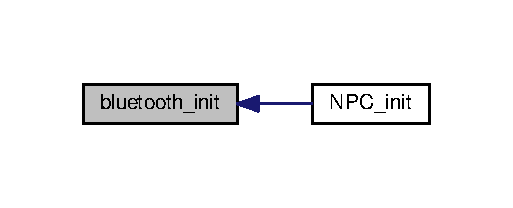
\includegraphics[width=246pt]{d7/d87/group__bluetooth___init_gaaa60810e0857e9e1e5b2cba80b8db3ff_icgraph}
\end{center}
\end{figure}


\index{Initialization and transmission handler functions@{Initialization and transmission handler functions}!D\+M\+A2\+\_\+\+Stream5\+\_\+\+I\+R\+Q\+Handler@{D\+M\+A2\+\_\+\+Stream5\+\_\+\+I\+R\+Q\+Handler}}
\index{D\+M\+A2\+\_\+\+Stream5\+\_\+\+I\+R\+Q\+Handler@{D\+M\+A2\+\_\+\+Stream5\+\_\+\+I\+R\+Q\+Handler}!Initialization and transmission handler functions@{Initialization and transmission handler functions}}
\subsubsection[{\texorpdfstring{D\+M\+A2\+\_\+\+Stream5\+\_\+\+I\+R\+Q\+Handler(void)}{DMA2_Stream5_IRQHandler(void)}}]{\setlength{\rightskip}{0pt plus 5cm}void D\+M\+A2\+\_\+\+Stream5\+\_\+\+I\+R\+Q\+Handler (
\begin{DoxyParamCaption}
\item[{void}]{}
\end{DoxyParamCaption}
)}\hypertarget{group__bluetooth___init_gaef190d87febc0414eb7a39bd4c2d2169}{}\label{group__bluetooth___init_gaef190d87febc0414eb7a39bd4c2d2169}


Global interrupt handler for D\+M\+A2 stream5. 

\begin{DoxyNote}{Note}
Except memcpy, there is no functions used to 
\end{DoxyNote}
Transfer could be completed by 2 events\+:
\begin{DoxyItemize}
\item All data actually transfered (N\+D\+TR = 0)
\item Stream disabled inside U\+S\+A\+RT I\+D\+LE line detected interrupt (N\+D\+TR != 0)
\end{DoxyItemize}

Definition at line 156 of file N\+P\+C\+\_\+bluetooth.\+c.

\index{Initialization and transmission handler functions@{Initialization and transmission handler functions}!U\+S\+A\+R\+T1\+\_\+\+I\+R\+Q\+Handler@{U\+S\+A\+R\+T1\+\_\+\+I\+R\+Q\+Handler}}
\index{U\+S\+A\+R\+T1\+\_\+\+I\+R\+Q\+Handler@{U\+S\+A\+R\+T1\+\_\+\+I\+R\+Q\+Handler}!Initialization and transmission handler functions@{Initialization and transmission handler functions}}
\subsubsection[{\texorpdfstring{U\+S\+A\+R\+T1\+\_\+\+I\+R\+Q\+Handler(void)}{USART1_IRQHandler(void)}}]{\setlength{\rightskip}{0pt plus 5cm}void U\+S\+A\+R\+T1\+\_\+\+I\+R\+Q\+Handler (
\begin{DoxyParamCaption}
\item[{void}]{}
\end{DoxyParamCaption}
)}\hypertarget{group__bluetooth___init_ga7139cd4baabbbcbab0c1fe6d7d4ae1cc}{}\label{group__bluetooth___init_ga7139cd4baabbbcbab0c1fe6d7d4ae1cc}


Global interrupt handler for U\+S\+A\+R\+T1. 



Definition at line 138 of file N\+P\+C\+\_\+bluetooth.\+c.


\hypertarget{group__bluetooth___trans}{}\section{Transmission functions}
\label{group__bluetooth___trans}\index{Transmission functions@{Transmission functions}}


bluetooth transmission functions  


Collaboration diagram for Transmission functions\+:\nopagebreak
\begin{figure}[H]
\begin{center}
\leavevmode
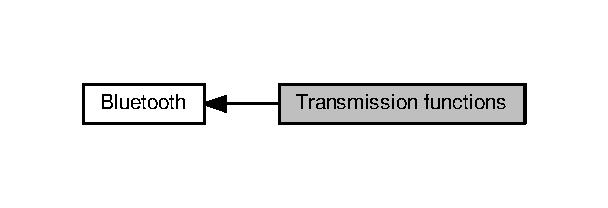
\includegraphics[width=292pt]{d5/d68/group__bluetooth___trans}
\end{center}
\end{figure}
\subsection*{Functions}
\begin{DoxyCompactItemize}
\item 
void \hyperlink{group__bluetooth___trans_ga31d829d5658369ee2c90b9c3cdbedfe1}{bluetooth\+\_\+send} (uint8\+\_\+t $\ast$data)
\begin{DoxyCompactList}\small\item\em send string to the hc-\/06 \end{DoxyCompactList}\end{DoxyCompactItemize}


\subsection{Detailed Description}
bluetooth transmission functions 



\subsection{Function Documentation}
\index{Transmission functions@{Transmission functions}!bluetooth\+\_\+send@{bluetooth\+\_\+send}}
\index{bluetooth\+\_\+send@{bluetooth\+\_\+send}!Transmission functions@{Transmission functions}}
\subsubsection[{\texorpdfstring{bluetooth\+\_\+send(uint8\+\_\+t $\ast$data)}{bluetooth_send(uint8_t *data)}}]{\setlength{\rightskip}{0pt plus 5cm}void bluetooth\+\_\+send (
\begin{DoxyParamCaption}
\item[{uint8\+\_\+t $\ast$}]{data}
\end{DoxyParamCaption}
)}\hypertarget{group__bluetooth___trans_ga31d829d5658369ee2c90b9c3cdbedfe1}{}\label{group__bluetooth___trans_ga31d829d5658369ee2c90b9c3cdbedfe1}


send string to the hc-\/06 


\begin{DoxyParams}{Parameters}
{\em data} & string to be sent \\
\hline
\end{DoxyParams}

\begin{DoxyRetVals}{Return values}
{\em None} & \\
\hline
\end{DoxyRetVals}


Definition at line 217 of file N\+P\+C\+\_\+bluetooth.\+c.


\hypertarget{group___r_t_c___p_r_e_d_i_v___definitions}{}\section{R\+T\+C\+\_\+\+P\+R\+E\+D\+I\+V\+\_\+\+Definitions}
\label{group___r_t_c___p_r_e_d_i_v___definitions}\index{R\+T\+C\+\_\+\+P\+R\+E\+D\+I\+V\+\_\+\+Definitions@{R\+T\+C\+\_\+\+P\+R\+E\+D\+I\+V\+\_\+\+Definitions}}


definition of prescaler for Asynchronous and Synchronous  


Collaboration diagram for R\+T\+C\+\_\+\+P\+R\+E\+D\+I\+V\+\_\+\+Definitions\+:
% FIG 0
\subsection*{Macros}
\begin{DoxyCompactItemize}
\item 
\mbox{\Hypertarget{group___r_t_c___p_r_e_d_i_v___definitions_ga7d28a18fc36cff684ad43ffd31ca45fc}\label{group___r_t_c___p_r_e_d_i_v___definitions_ga7d28a18fc36cff684ad43ffd31ca45fc}} 
\#define {\bfseries R\+T\+C\+\_\+\+P\+R\+E\+D\+I\+V\+\_\+A}~0x7C
\item 
\mbox{\Hypertarget{group___r_t_c___p_r_e_d_i_v___definitions_ga3578b56bdfe76014a3af7e276fe6a6e4}\label{group___r_t_c___p_r_e_d_i_v___definitions_ga3578b56bdfe76014a3af7e276fe6a6e4}} 
\#define {\bfseries R\+T\+C\+\_\+\+P\+R\+E\+D\+I\+V\+\_\+S}~0\+X1\+F3F
\end{DoxyCompactItemize}


\subsection{Detailed Description}
definition of prescaler for Asynchronous and Synchronous 


\hypertarget{group___c_l_o_c_k___choice}{}\section{C\+L\+O\+C\+K\+\_\+\+Choice}
\label{group___c_l_o_c_k___choice}\index{C\+L\+O\+C\+K\+\_\+\+Choice@{C\+L\+O\+C\+K\+\_\+\+Choice}}


Clock A or B.  


\subsection*{Macros}
\begin{DoxyCompactItemize}
\item 
\mbox{\Hypertarget{group___c_l_o_c_k___choice_gaa6850d52f4718938783dcc4b932f78ac}\label{group___c_l_o_c_k___choice_gaa6850d52f4718938783dcc4b932f78ac}} 
\#define {\bfseries C\+L\+O\+C\+K\+\_\+A}~R\+T\+C\+\_\+\+Alarm\+\_\+A
\item 
\mbox{\Hypertarget{group___c_l_o_c_k___choice_gaa955d6afa2e3fcc5dc68064b9cd5161f}\label{group___c_l_o_c_k___choice_gaa955d6afa2e3fcc5dc68064b9cd5161f}} 
\#define {\bfseries C\+L\+O\+C\+K\+\_\+B}~R\+T\+C\+\_\+\+Alarm\+\_\+B
\end{DoxyCompactItemize}


\subsection{Detailed Description}
Clock A or B. 


\hypertarget{group___c_l_o_c_k___format}{}\section{C\+L\+O\+C\+K\+\_\+\+Format}
\label{group___c_l_o_c_k___format}\index{C\+L\+O\+C\+K\+\_\+\+Format@{C\+L\+O\+C\+K\+\_\+\+Format}}


AM or PM.  


Collaboration diagram for C\+L\+O\+C\+K\+\_\+\+Format\+:
% FIG 0
\subsection*{Macros}
\begin{DoxyCompactItemize}
\item 
\mbox{\Hypertarget{group___c_l_o_c_k___format_gae4cd6ada23b2e1749a2fd828cba94f5a}\label{group___c_l_o_c_k___format_gae4cd6ada23b2e1749a2fd828cba94f5a}} 
\#define {\bfseries C\+L\+O\+C\+K\+\_\+\+AM}~R\+T\+C\+\_\+\+H12\+\_\+\+AM
\item 
\mbox{\Hypertarget{group___c_l_o_c_k___format_ga8978739eedb215b454cc9615031685d9}\label{group___c_l_o_c_k___format_ga8978739eedb215b454cc9615031685d9}} 
\#define {\bfseries C\+L\+O\+C\+K\+\_\+\+PM}~R\+T\+C\+\_\+\+H12\+\_\+\+PM
\end{DoxyCompactItemize}


\subsection{Detailed Description}
AM or PM. 


\hypertarget{group___c_l_o_c_k___value}{}\section{C\+L\+O\+C\+K\+\_\+\+Value}
\label{group___c_l_o_c_k___value}\index{C\+L\+O\+C\+K\+\_\+\+Value@{C\+L\+O\+C\+K\+\_\+\+Value}}


Access time or date parameters.  


Collaboration diagram for C\+L\+O\+C\+K\+\_\+\+Value\+:
% FIG 0
\subsection*{Macros}
\begin{DoxyCompactItemize}
\item 
\mbox{\Hypertarget{group___c_l_o_c_k___value_ga41cab09c59fe3cc9a25719ec3be3fd4d}\label{group___c_l_o_c_k___value_ga41cab09c59fe3cc9a25719ec3be3fd4d}} 
\#define {\bfseries C\+L\+O\+C\+K\+\_\+\+Week\+Day}~(uint8\+\_\+t) (\hyperlink{group___clock___time___date_gabb4d72928cb3d131d40067fb141003aa}{clock\+\_\+get\+Date}() $>$$>$ 24)
\item 
\mbox{\Hypertarget{group___c_l_o_c_k___value_gabd717170aa836b16355413e2c5ca0ad8}\label{group___c_l_o_c_k___value_gabd717170aa836b16355413e2c5ca0ad8}} 
\#define {\bfseries C\+L\+O\+C\+K\+\_\+\+Month}~(uint8\+\_\+t) (\hyperlink{group___clock___time___date_gabb4d72928cb3d131d40067fb141003aa}{clock\+\_\+get\+Date}() $>$$>$ 16)
\item 
\mbox{\Hypertarget{group___c_l_o_c_k___value_gaad5816af032bcc19c84bc93e03f42236}\label{group___c_l_o_c_k___value_gaad5816af032bcc19c84bc93e03f42236}} 
\#define {\bfseries C\+L\+O\+C\+K\+\_\+date}~(uint8\+\_\+t) (\hyperlink{group___clock___time___date_gabb4d72928cb3d131d40067fb141003aa}{clock\+\_\+get\+Date}() $>$$>$ 8)
\item 
\mbox{\Hypertarget{group___c_l_o_c_k___value_ga35866274a21e8d3c0223c465209f3d74}\label{group___c_l_o_c_k___value_ga35866274a21e8d3c0223c465209f3d74}} 
\#define {\bfseries C\+L\+O\+C\+K\+\_\+\+Year}~(uint8\+\_\+t) \hyperlink{group___clock___time___date_gabb4d72928cb3d131d40067fb141003aa}{clock\+\_\+get\+Date}()
\item 
\mbox{\Hypertarget{group___c_l_o_c_k___value_ga49ea807900604714bab70a531081ac6a}\label{group___c_l_o_c_k___value_ga49ea807900604714bab70a531081ac6a}} 
\#define {\bfseries C\+L\+O\+C\+K\+\_\+\+Hours}~(uint8\+\_\+t) (\hyperlink{group___clock___time___date_ga03ae6948083c259f6edc0b146f40dc62}{clock\+\_\+get\+Time}() $>$$>$ 24)
\item 
\mbox{\Hypertarget{group___c_l_o_c_k___value_ga302d9ee9e79c96969e558b9ffdba3212}\label{group___c_l_o_c_k___value_ga302d9ee9e79c96969e558b9ffdba3212}} 
\#define {\bfseries C\+L\+O\+C\+K\+\_\+\+Minutes}~(uint8\+\_\+t) (\hyperlink{group___clock___time___date_ga03ae6948083c259f6edc0b146f40dc62}{clock\+\_\+get\+Time}() $>$$>$ 16)
\item 
\mbox{\Hypertarget{group___c_l_o_c_k___value_gaa6d6eb65ec4fce5bfef7fb6edf5d2620}\label{group___c_l_o_c_k___value_gaa6d6eb65ec4fce5bfef7fb6edf5d2620}} 
\#define {\bfseries C\+L\+O\+C\+K\+\_\+seconds}~(uint8\+\_\+t) (\hyperlink{group___clock___time___date_ga03ae6948083c259f6edc0b146f40dc62}{clock\+\_\+get\+Time}() $>$$>$ 8)
\item 
\mbox{\Hypertarget{group___c_l_o_c_k___value_gafec8368ed05e06cadccc3becf2cd0ead}\label{group___c_l_o_c_k___value_gafec8368ed05e06cadccc3becf2cd0ead}} 
\#define {\bfseries C\+L\+O\+C\+K\+\_\+\+Format}~(uint8\+\_\+t) \hyperlink{group___clock___time___date_ga03ae6948083c259f6edc0b146f40dc62}{clock\+\_\+get\+Time}()
\end{DoxyCompactItemize}


\subsection{Detailed Description}
Access time or date parameters. 


\hypertarget{group___r_e_p_e_a_t___definitions}{}\section{R\+E\+P\+E\+A\+T\+\_\+\+Definitions}
\label{group___r_e_p_e_a_t___definitions}\index{R\+E\+P\+E\+A\+T\+\_\+\+Definitions@{R\+E\+P\+E\+A\+T\+\_\+\+Definitions}}


Alarm repeat options.  


Collaboration diagram for R\+E\+P\+E\+A\+T\+\_\+\+Definitions\+:
% FIG 0
\subsection*{Macros}
\begin{DoxyCompactItemize}
\item 
\mbox{\Hypertarget{group___r_e_p_e_a_t___definitions_ga9f2fcc8488db26c77b5ffd8f6c10c5d0}\label{group___r_e_p_e_a_t___definitions_ga9f2fcc8488db26c77b5ffd8f6c10c5d0}} 
\#define {\bfseries R\+E\+P\+E\+A\+T\+\_\+\+Date\+Week\+Day}~(uint32\+\_\+t) R\+T\+C\+\_\+\+Alarm\+Mask\+\_\+\+Date\+Week\+Day
\item 
\mbox{\Hypertarget{group___r_e_p_e_a_t___definitions_gaa31a39c1b2a1d619db0901cc7c8d4592}\label{group___r_e_p_e_a_t___definitions_gaa31a39c1b2a1d619db0901cc7c8d4592}} 
\#define {\bfseries R\+E\+P\+E\+A\+T\+\_\+\+Hours}~(uint32\+\_\+t) R\+T\+C\+\_\+\+Alarm\+Mask\+\_\+\+Hours
\item 
\mbox{\Hypertarget{group___r_e_p_e_a_t___definitions_gac80fc7d65b83128ca58e210922020d37}\label{group___r_e_p_e_a_t___definitions_gac80fc7d65b83128ca58e210922020d37}} 
\#define {\bfseries R\+E\+P\+E\+A\+T\+\_\+\+Minutes}~(uint32\+\_\+t) R\+T\+C\+\_\+\+Alarm\+Mask\+\_\+\+Minutes
\item 
\mbox{\Hypertarget{group___r_e_p_e_a_t___definitions_ga12d07c13f393b5b12efad9cd892de472}\label{group___r_e_p_e_a_t___definitions_ga12d07c13f393b5b12efad9cd892de472}} 
\#define {\bfseries R\+E\+P\+E\+A\+T\+\_\+\+Seconds}~(uint32\+\_\+t) R\+T\+C\+\_\+\+Alarm\+Mask\+\_\+\+Seconds
\item 
\mbox{\Hypertarget{group___r_e_p_e_a_t___definitions_ga473d162f72a4680e7e14043dfaf092c0}\label{group___r_e_p_e_a_t___definitions_ga473d162f72a4680e7e14043dfaf092c0}} 
\#define {\bfseries R\+E\+P\+E\+A\+T\+\_\+\+None}~(uint32\+\_\+t) R\+T\+C\+\_\+\+Alarm\+Mask\+\_\+\+None
\end{DoxyCompactItemize}


\subsection{Detailed Description}
Alarm repeat options. 


\hypertarget{group___clock___init}{}\section{Initialisation functions}
\label{group___clock___init}\index{Initialisation functions@{Initialisation functions}}


Clock initialisation functions.  


Collaboration diagram for Initialisation functions\+:\nopagebreak
\begin{figure}[H]
\begin{center}
\leavevmode
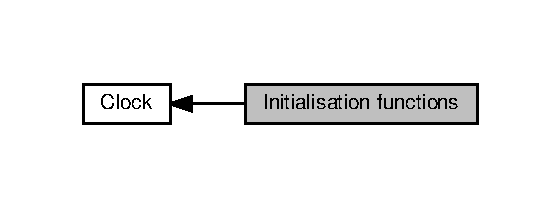
\includegraphics[width=269pt]{dd/d06/group___clock___init}
\end{center}
\end{figure}
\subsection*{Functions}
\begin{DoxyCompactItemize}
\item 
void \hyperlink{group___clock___init_ga78ab77b57cf2e00089f0a3a22508524c}{clock\+\_\+init} (void)
\begin{DoxyCompactList}\small\item\em Initialise the clock to 1\+Hz and setup peripherals for Alarm. \end{DoxyCompactList}\end{DoxyCompactItemize}


\subsection{Detailed Description}
Clock initialisation functions. 



\subsection{Function Documentation}
\index{Initialisation functions@{Initialisation functions}!clock\+\_\+init@{clock\+\_\+init}}
\index{clock\+\_\+init@{clock\+\_\+init}!Initialisation functions@{Initialisation functions}}
\subsubsection[{\texorpdfstring{clock\+\_\+init(void)}{clock_init(void)}}]{\setlength{\rightskip}{0pt plus 5cm}void clock\+\_\+init (
\begin{DoxyParamCaption}
\item[{void}]{}
\end{DoxyParamCaption}
)}\hypertarget{group___clock___init_ga78ab77b57cf2e00089f0a3a22508524c}{}\label{group___clock___init_ga78ab77b57cf2e00089f0a3a22508524c}


Initialise the clock to 1\+Hz and setup peripherals for Alarm. 


\begin{DoxyParams}{Parameters}
{\em None} & \\
\hline
\end{DoxyParams}

\begin{DoxyRetVals}{Return values}
{\em None} & \\
\hline
\end{DoxyRetVals}


Definition at line 74 of file N\+P\+C\+\_\+clock.\+c.



Here is the caller graph for this function\+:\nopagebreak
\begin{figure}[H]
\begin{center}
\leavevmode
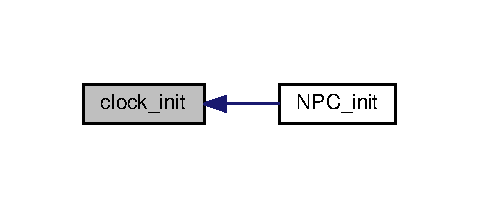
\includegraphics[width=230pt]{dd/d06/group___clock___init_ga78ab77b57cf2e00089f0a3a22508524c_icgraph}
\end{center}
\end{figure}



\hypertarget{group___clock___time___date}{}\section{Time and Date Configuration functions}
\label{group___clock___time___date}\index{Time and Date Configuration functions@{Time and Date Configuration functions}}


Clock time and date configuration functions.  


\subsection*{Functions}
\begin{DoxyCompactItemize}
\item 
Error\+Status \hyperlink{group___clock___time___date_gaf16498fa2702bfda6b89a3335ccc7ca6}{clock\+\_\+set\+Date} (uint8\+\_\+t week\+Day, uint8\+\_\+t month, uint8\+\_\+t date, uint8\+\_\+t year)
\begin{DoxyCompactList}\small\item\em Set the clock\textquotesingle{}s date. \end{DoxyCompactList}\item 
Error\+Status \hyperlink{group___clock___time___date_ga11404197d58ddf6b46230bcde4282ef2}{clock\+\_\+set\+Time} (uint8\+\_\+t am\+\_\+pm, uint8\+\_\+t hours, uint8\+\_\+t minutes, uint8\+\_\+t second)
\begin{DoxyCompactList}\small\item\em Set the clock\textquotesingle{}s time. \end{DoxyCompactList}\item 
uint32\+\_\+t \hyperlink{group___clock___time___date_gabb4d72928cb3d131d40067fb141003aa}{clock\+\_\+get\+Date} (void)
\begin{DoxyCompactList}\small\item\em Get the date encoded in a 32b format. \end{DoxyCompactList}\item 
uint32\+\_\+t \hyperlink{group___clock___time___date_ga03ae6948083c259f6edc0b146f40dc62}{clock\+\_\+get\+Time} (void)
\begin{DoxyCompactList}\small\item\em Get the time encoded in a 32b format. \end{DoxyCompactList}\end{DoxyCompactItemize}


\subsection{Detailed Description}
Clock time and date configuration functions. 



\subsection{Function Documentation}
\mbox{\Hypertarget{group___clock___time___date_gabb4d72928cb3d131d40067fb141003aa}\label{group___clock___time___date_gabb4d72928cb3d131d40067fb141003aa}} 
\index{Time and Date Configuration functions@{Time and Date Configuration functions}!clock\+\_\+get\+Date@{clock\+\_\+get\+Date}}
\index{clock\+\_\+get\+Date@{clock\+\_\+get\+Date}!Time and Date Configuration functions@{Time and Date Configuration functions}}
\subsubsection{\texorpdfstring{clock\+\_\+get\+Date()}{clock\_getDate()}}
{\footnotesize\ttfamily uint32\+\_\+t clock\+\_\+get\+Date (\begin{DoxyParamCaption}\item[{void}]{ }\end{DoxyParamCaption})}



Get the date encoded in a 32b format. 


\begin{DoxyParams}{Parameters}
{\em None} & \\
\hline
\end{DoxyParams}

\begin{DoxyRetVals}{Return values}
{\em An} & uint32\+\_\+t containing the week\+Day as its M\+B3, date \+: M\+B2, month \+: M\+B1, year \+: M\+B0 \\
\hline
\end{DoxyRetVals}
\mbox{\Hypertarget{group___clock___time___date_ga03ae6948083c259f6edc0b146f40dc62}\label{group___clock___time___date_ga03ae6948083c259f6edc0b146f40dc62}} 
\index{Time and Date Configuration functions@{Time and Date Configuration functions}!clock\+\_\+get\+Time@{clock\+\_\+get\+Time}}
\index{clock\+\_\+get\+Time@{clock\+\_\+get\+Time}!Time and Date Configuration functions@{Time and Date Configuration functions}}
\subsubsection{\texorpdfstring{clock\+\_\+get\+Time()}{clock\_getTime()}}
{\footnotesize\ttfamily uint32\+\_\+t clock\+\_\+get\+Time (\begin{DoxyParamCaption}\item[{void}]{ }\end{DoxyParamCaption})}



Get the time encoded in a 32b format. 


\begin{DoxyParams}{Parameters}
{\em None} & \\
\hline
\end{DoxyParams}

\begin{DoxyRetVals}{Return values}
{\em An} & uint32\+\_\+t containing the hour as its M\+B3, minutes \+: M\+B2, Seconds \+: M\+B1, format \+: M\+B0 \\
\hline
\end{DoxyRetVals}
\mbox{\Hypertarget{group___clock___time___date_gaf16498fa2702bfda6b89a3335ccc7ca6}\label{group___clock___time___date_gaf16498fa2702bfda6b89a3335ccc7ca6}} 
\index{Time and Date Configuration functions@{Time and Date Configuration functions}!clock\+\_\+set\+Date@{clock\+\_\+set\+Date}}
\index{clock\+\_\+set\+Date@{clock\+\_\+set\+Date}!Time and Date Configuration functions@{Time and Date Configuration functions}}
\subsubsection{\texorpdfstring{clock\+\_\+set\+Date()}{clock\_setDate()}}
{\footnotesize\ttfamily Error\+Status clock\+\_\+set\+Date (\begin{DoxyParamCaption}\item[{uint8\+\_\+t}]{week\+Day,  }\item[{uint8\+\_\+t}]{month,  }\item[{uint8\+\_\+t}]{date,  }\item[{uint8\+\_\+t}]{year }\end{DoxyParamCaption})}



Set the clock\textquotesingle{}s date. 


\begin{DoxyParams}{Parameters}
{\em None} & \\
\hline
\end{DoxyParams}

\begin{DoxyRetVals}{Return values}
{\em Error\+Status} & representing the outcome of the operation
\begin{DoxyItemize}
\item S\+U\+C\+C\+E\+SS\+: R\+TC Shift registers are configured
\item E\+R\+R\+OR\+: R\+TC Shift registers are not configured 
\end{DoxyItemize}\\
\hline
\end{DoxyRetVals}
\mbox{\Hypertarget{group___clock___time___date_ga11404197d58ddf6b46230bcde4282ef2}\label{group___clock___time___date_ga11404197d58ddf6b46230bcde4282ef2}} 
\index{Time and Date Configuration functions@{Time and Date Configuration functions}!clock\+\_\+set\+Time@{clock\+\_\+set\+Time}}
\index{clock\+\_\+set\+Time@{clock\+\_\+set\+Time}!Time and Date Configuration functions@{Time and Date Configuration functions}}
\subsubsection{\texorpdfstring{clock\+\_\+set\+Time()}{clock\_setTime()}}
{\footnotesize\ttfamily Error\+Status clock\+\_\+set\+Time (\begin{DoxyParamCaption}\item[{uint8\+\_\+t}]{am\+\_\+pm,  }\item[{uint8\+\_\+t}]{hours,  }\item[{uint8\+\_\+t}]{minutes,  }\item[{uint8\+\_\+t}]{second }\end{DoxyParamCaption})}



Set the clock\textquotesingle{}s time. 


\begin{DoxyParams}{Parameters}
{\em None} & \\
\hline
\end{DoxyParams}

\begin{DoxyRetVals}{Return values}
{\em Error\+Status} & representing the outcome of the operation
\begin{DoxyItemize}
\item S\+U\+C\+C\+E\+SS\+: R\+TC Shift registers are configured
\item E\+R\+R\+OR\+: R\+TC Shift registers are not configured 
\end{DoxyItemize}\\
\hline
\end{DoxyRetVals}

\hypertarget{group___clock___alarms}{}\section{Alarms configuration functions}
\label{group___clock___alarms}\index{Alarms configuration functions@{Alarms configuration functions}}


Clock alarm configuration functions.  


\subsection*{Functions}
\begin{DoxyCompactItemize}
\item 
R\+T\+C\+\_\+\+Alarm\+Type\+Def \hyperlink{group___clock___alarms_ga5e1614dbb1a210106dbade3f133db27e}{clock\+\_\+create\+Alarm} (uint8\+\_\+t am\+\_\+pm, uint8\+\_\+t hours, uint8\+\_\+t minutes, uint8\+\_\+t seconds, uint32\+\_\+t date\+Week\+Day\+Sel, uint8\+\_\+t date\+Week\+Day, uint32\+\_\+t repeat)
\begin{DoxyCompactList}\small\item\em Create an Alarm Structure given all the parameters. \end{DoxyCompactList}\item 
void \hyperlink{group___clock___alarms_gab56f512746d4f2638232db28bb7dac2b}{clock\+\_\+setA} (R\+T\+C\+\_\+\+Alarm\+Type\+Def $\ast$Alarm)
\begin{DoxyCompactList}\small\item\em Set an alarm to R\+T\+C\+\_\+\+Alarm\+\_\+A, given a Alarm structure R\+T\+C\+\_\+\+Alarm\+Type\+Def. \end{DoxyCompactList}\item 
void \hyperlink{group___clock___alarms_gaea1a099c4ad6de8b99517ac6453e3569}{clock\+\_\+set\+Alarm} (uint8\+\_\+t am\+\_\+pm, uint8\+\_\+t hours, uint8\+\_\+t minutes, uint8\+\_\+t seconds, uint32\+\_\+t date\+Week\+Day\+Sel, uint8\+\_\+t date\+Week\+Day, uint32\+\_\+t repeat)
\begin{DoxyCompactList}\small\item\em Set an alarm to R\+T\+C\+\_\+\+Alarm\+\_\+A, given all the alarm parameters. \end{DoxyCompactList}\item 
void \hyperlink{group___clock___alarms_ga4da4fb52ec579671d337938e78f9a207}{R\+T\+C\+\_\+\+Alarm\+\_\+\+I\+R\+Q\+Handler} (void)
\begin{DoxyCompactList}\small\item\em Alarm Handler. \end{DoxyCompactList}\end{DoxyCompactItemize}


\subsection{Detailed Description}
Clock alarm configuration functions. 



\subsection{Function Documentation}
\mbox{\Hypertarget{group___clock___alarms_ga5e1614dbb1a210106dbade3f133db27e}\label{group___clock___alarms_ga5e1614dbb1a210106dbade3f133db27e}} 
\index{Alarms configuration functions@{Alarms configuration functions}!clock\+\_\+create\+Alarm@{clock\+\_\+create\+Alarm}}
\index{clock\+\_\+create\+Alarm@{clock\+\_\+create\+Alarm}!Alarms configuration functions@{Alarms configuration functions}}
\subsubsection{\texorpdfstring{clock\+\_\+create\+Alarm()}{clock\_createAlarm()}}
{\footnotesize\ttfamily R\+T\+C\+\_\+\+Alarm\+Type\+Def clock\+\_\+create\+Alarm (\begin{DoxyParamCaption}\item[{uint8\+\_\+t}]{am\+\_\+pm,  }\item[{uint8\+\_\+t}]{hours,  }\item[{uint8\+\_\+t}]{minutes,  }\item[{uint8\+\_\+t}]{seconds,  }\item[{uint32\+\_\+t}]{date\+Week\+Day\+Sel,  }\item[{uint8\+\_\+t}]{date\+Week\+Day,  }\item[{uint32\+\_\+t}]{repeat }\end{DoxyParamCaption})}



Create an Alarm Structure given all the parameters. 


\begin{DoxyParams}{Parameters}
{\em am\+\_\+pm} & AM PM format (C\+L\+O\+C\+K\+\_\+\+AM) \\
\hline
{\em hours} & Alarm hours \\
\hline
{\em minutes} & Alarm minutes \\
\hline
{\em seconds} & Alarm seconds \\
\hline
{\em date\+Week\+Day\+Sel} & Date of Week\+Day selection R\+T\+C\+\_\+\+Alarm\+Date\+Week\+Day\+\_\+\+Definitions \\
\hline
{\em date\+Week\+Day} & Specify Alarm Date/\+Weekday if Date then value range from 1-\/31, else R\+T\+C\+\_\+\+Week\+Day\+\_\+\+Definitions \\
\hline
{\em repeat} & Specify the repetition of the Alarm \\
\hline
\end{DoxyParams}

\begin{DoxyRetVals}{Return values}
{\em An} & R\+T\+C\+\_\+\+Alarm\+Type\+Def containing all the parameters above \\
\hline
\end{DoxyRetVals}
\mbox{\Hypertarget{group___clock___alarms_gab56f512746d4f2638232db28bb7dac2b}\label{group___clock___alarms_gab56f512746d4f2638232db28bb7dac2b}} 
\index{Alarms configuration functions@{Alarms configuration functions}!clock\+\_\+setA@{clock\+\_\+setA}}
\index{clock\+\_\+setA@{clock\+\_\+setA}!Alarms configuration functions@{Alarms configuration functions}}
\subsubsection{\texorpdfstring{clock\+\_\+set\+A()}{clock\_setA()}}
{\footnotesize\ttfamily void clock\+\_\+setA (\begin{DoxyParamCaption}\item[{R\+T\+C\+\_\+\+Alarm\+Type\+Def $\ast$}]{Alarm }\end{DoxyParamCaption})}



Set an alarm to R\+T\+C\+\_\+\+Alarm\+\_\+A, given a Alarm structure R\+T\+C\+\_\+\+Alarm\+Type\+Def. 


\begin{DoxyParams}{Parameters}
{\em Alarm} & A pointer to the R\+T\+C\+\_\+\+Alarm\+Type\+Def \\
\hline
\end{DoxyParams}

\begin{DoxyRetVals}{Return values}
{\em None} & \\
\hline
\end{DoxyRetVals}
\mbox{\Hypertarget{group___clock___alarms_gaea1a099c4ad6de8b99517ac6453e3569}\label{group___clock___alarms_gaea1a099c4ad6de8b99517ac6453e3569}} 
\index{Alarms configuration functions@{Alarms configuration functions}!clock\+\_\+set\+Alarm@{clock\+\_\+set\+Alarm}}
\index{clock\+\_\+set\+Alarm@{clock\+\_\+set\+Alarm}!Alarms configuration functions@{Alarms configuration functions}}
\subsubsection{\texorpdfstring{clock\+\_\+set\+Alarm()}{clock\_setAlarm()}}
{\footnotesize\ttfamily void clock\+\_\+set\+Alarm (\begin{DoxyParamCaption}\item[{uint8\+\_\+t}]{am\+\_\+pm,  }\item[{uint8\+\_\+t}]{hours,  }\item[{uint8\+\_\+t}]{minutes,  }\item[{uint8\+\_\+t}]{seconds,  }\item[{uint32\+\_\+t}]{date\+Week\+Day\+Sel,  }\item[{uint8\+\_\+t}]{date\+Week\+Day,  }\item[{uint32\+\_\+t}]{repeat }\end{DoxyParamCaption})}



Set an alarm to R\+T\+C\+\_\+\+Alarm\+\_\+A, given all the alarm parameters. 


\begin{DoxyParams}{Parameters}
{\em am\+\_\+pm} & AM PM format (C\+L\+O\+C\+K\+\_\+\+AM) \\
\hline
{\em hours} & Alarm hours \\
\hline
{\em minutes} & Alarm minutes \\
\hline
{\em seconds} & Alarm seconds \\
\hline
{\em date\+Week\+Day\+Sel} & Date of Week\+Day selection R\+T\+C\+\_\+\+Alarm\+Date\+Week\+Day\+\_\+\+Definitions \\
\hline
{\em date\+Week\+Day} & Specify Alarm Date/\+Weekday if Date then value range from 1-\/31, else R\+T\+C\+\_\+\+Week\+Day\+\_\+\+Definitions \\
\hline
{\em repeat} & Specify the repetition of the Alarm \\
\hline
\end{DoxyParams}

\begin{DoxyRetVals}{Return values}
{\em None} & \\
\hline
\end{DoxyRetVals}
\mbox{\Hypertarget{group___clock___alarms_ga4da4fb52ec579671d337938e78f9a207}\label{group___clock___alarms_ga4da4fb52ec579671d337938e78f9a207}} 
\index{Alarms configuration functions@{Alarms configuration functions}!R\+T\+C\+\_\+\+Alarm\+\_\+\+I\+R\+Q\+Handler@{R\+T\+C\+\_\+\+Alarm\+\_\+\+I\+R\+Q\+Handler}}
\index{R\+T\+C\+\_\+\+Alarm\+\_\+\+I\+R\+Q\+Handler@{R\+T\+C\+\_\+\+Alarm\+\_\+\+I\+R\+Q\+Handler}!Alarms configuration functions@{Alarms configuration functions}}
\subsubsection{\texorpdfstring{R\+T\+C\+\_\+\+Alarm\+\_\+\+I\+R\+Q\+Handler()}{RTC\_Alarm\_IRQHandler()}}
{\footnotesize\ttfamily void R\+T\+C\+\_\+\+Alarm\+\_\+\+I\+R\+Q\+Handler (\begin{DoxyParamCaption}\item[{void}]{ }\end{DoxyParamCaption})}



Alarm Handler. 


\begin{DoxyParams}{Parameters}
{\em None} & \\
\hline
\end{DoxyParams}

\begin{DoxyRetVals}{Return values}
{\em None} & \\
\hline
\end{DoxyRetVals}

\hypertarget{group___instructions}{}\section{Instructions}
\label{group___instructions}\index{Instructions@{Instructions}}


25\+L\+C640A instruction set  


Collaboration diagram for Instructions\+:
% FIG 0
\subsection*{Macros}
\begin{DoxyCompactItemize}
\item 
\mbox{\Hypertarget{group___instructions_ga53dec1d28a7c7b24b2d56c058f7e140a}\label{group___instructions_ga53dec1d28a7c7b24b2d56c058f7e140a}} 
\#define {\bfseries W\+R\+EN}~0b00000110
\item 
\mbox{\Hypertarget{group___instructions_gacb229428140f30a6f8b6fa2ebb3fb6f0}\label{group___instructions_gacb229428140f30a6f8b6fa2ebb3fb6f0}} 
\#define {\bfseries W\+R\+DI}~0b00000100
\item 
\mbox{\Hypertarget{group___instructions_ga899f71cf1ab9be6e8c8482e443558450}\label{group___instructions_ga899f71cf1ab9be6e8c8482e443558450}} 
\#define {\bfseries R\+D\+SR}~0b00000101
\item 
\mbox{\Hypertarget{group___instructions_ga29d01dca16eb0a060d2efd567b58b47a}\label{group___instructions_ga29d01dca16eb0a060d2efd567b58b47a}} 
\#define {\bfseries W\+R\+SR}~0b00000001
\item 
\mbox{\Hypertarget{group___instructions_gada74e7db007a68e763f20c17f2985356}\label{group___instructions_gada74e7db007a68e763f20c17f2985356}} 
\#define {\bfseries R\+E\+AD}~0b00000011
\item 
\mbox{\Hypertarget{group___instructions_gaa10f470e996d0f51210d24f442d25e1e}\label{group___instructions_gaa10f470e996d0f51210d24f442d25e1e}} 
\#define {\bfseries W\+R\+I\+TE}~0b00000010
\end{DoxyCompactItemize}


\subsection{Detailed Description}
25\+L\+C640A instruction set 


\hypertarget{group___utilities}{}\section{Utilities}
\label{group___utilities}\index{Utilities@{Utilities}}
\subsection*{Macros}
\begin{DoxyCompactItemize}
\item 
\mbox{\Hypertarget{group___utilities_gaa583f25d8bd438def94d50dff97b468d}\label{group___utilities_gaa583f25d8bd438def94d50dff97b468d}} 
\#define {\bfseries P\+A\+G\+E\+\_\+\+L\+E\+N\+G\+TH}~32
\end{DoxyCompactItemize}


\subsection{Detailed Description}

\hypertarget{group___eeprom___init}{}\section{Initialisation functions}
\label{group___eeprom___init}\index{Initialisation functions@{Initialisation functions}}


Eeprom initialisation functions.  


Collaboration diagram for Initialisation functions\+:\nopagebreak
\begin{figure}[H]
\begin{center}
\leavevmode
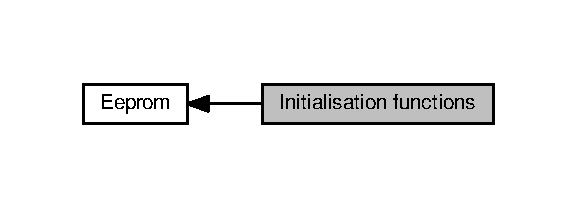
\includegraphics[width=277pt]{d7/d63/group___eeprom___init}
\end{center}
\end{figure}
\subsection*{Functions}
\begin{DoxyCompactItemize}
\item 
void \hyperlink{group___eeprom___init_ga4ec7f9d780da432051aa74ec5892a94c}{eeprom\+\_\+init} (void)
\begin{DoxyCompactList}\small\item\em Initialise communication to the eeprom. \end{DoxyCompactList}\end{DoxyCompactItemize}


\subsection{Detailed Description}
Eeprom initialisation functions. 



\subsection{Function Documentation}
\index{Initialisation functions@{Initialisation functions}!eeprom\+\_\+init@{eeprom\+\_\+init}}
\index{eeprom\+\_\+init@{eeprom\+\_\+init}!Initialisation functions@{Initialisation functions}}
\subsubsection[{\texorpdfstring{eeprom\+\_\+init(void)}{eeprom_init(void)}}]{\setlength{\rightskip}{0pt plus 5cm}void eeprom\+\_\+init (
\begin{DoxyParamCaption}
\item[{void}]{}
\end{DoxyParamCaption}
)}\hypertarget{group___eeprom___init_ga4ec7f9d780da432051aa74ec5892a94c}{}\label{group___eeprom___init_ga4ec7f9d780da432051aa74ec5892a94c}


Initialise communication to the eeprom. 


\begin{DoxyParams}{Parameters}
{\em None} & \\
\hline
\end{DoxyParams}

\begin{DoxyRetVals}{Return values}
{\em None} & \\
\hline
\end{DoxyRetVals}


Definition at line 48 of file N\+P\+C\+\_\+eeprom.\+c.



Here is the caller graph for this function\+:\nopagebreak
\begin{figure}[H]
\begin{center}
\leavevmode
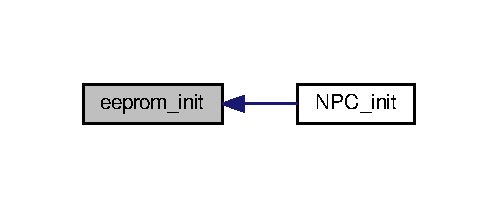
\includegraphics[width=239pt]{d7/d63/group___eeprom___init_ga4ec7f9d780da432051aa74ec5892a94c_icgraph}
\end{center}
\end{figure}



\hypertarget{group___eeprom___trans}{}\section{Transmission functions}
\label{group___eeprom___trans}\index{Transmission functions@{Transmission functions}}


Eeprom data transmission functions.  


Collaboration diagram for Transmission functions\+:\nopagebreak
\begin{figure}[H]
\begin{center}
\leavevmode
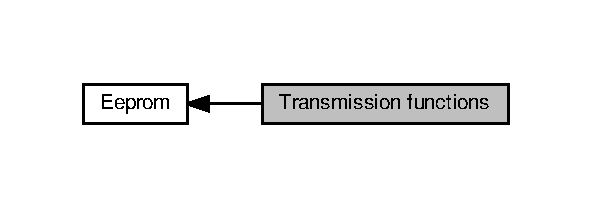
\includegraphics[width=284pt]{d2/de3/group___eeprom___trans}
\end{center}
\end{figure}
\subsection*{Functions}
\begin{DoxyCompactItemize}
\item 
Error\+Status \hyperlink{group___eeprom___trans_ga46c7b6081a89f96d53b6ebc0d0b6f60b}{eeprom\+\_\+write} (uint16\+\_\+t address, uint8\+\_\+t data)
\begin{DoxyCompactList}\small\item\em Write a byte to the eeprom. \end{DoxyCompactList}\item 
uint8\+\_\+t \hyperlink{group___eeprom___trans_gafaa7cca6f6ad1d9ae49522324c825c2f}{eeprom\+\_\+read} (uint16\+\_\+t address)
\begin{DoxyCompactList}\small\item\em Read a byte from the eeprom. \end{DoxyCompactList}\item 
Error\+Status \hyperlink{group___eeprom___trans_ga8c4d6169df1fdb9baeca667b5e9b0058}{eeprom\+\_\+write32\+Bytes} (uint16\+\_\+t base\+Address, uint8\+\_\+t $\ast$data)
\begin{DoxyCompactList}\small\item\em Write a page to the eeprom. \end{DoxyCompactList}\item 
uint32\+\_\+t \hyperlink{group___eeprom___trans_ga9a323370ddd02d91c6118f104c015b43}{eeprom\+\_\+read4\+Bytes} (uint16\+\_\+t base\+Address)
\begin{DoxyCompactList}\small\item\em Read a 32byte from eeprom. \end{DoxyCompactList}\item 
Error\+Status \hyperlink{group___eeprom___trans_ga9dea9d824339ffc184a047749533b96d}{eeprom\+\_\+write\+N\+Bytes} (uint16\+\_\+t base\+Address, uint8\+\_\+t $\ast$data, uint16\+\_\+t N)
\begin{DoxyCompactList}\small\item\em Write N bytes to the eeprom. \end{DoxyCompactList}\item 
Error\+Status \hyperlink{group___eeprom___trans_ga7d9db4a4822fa0c3e5b811615aaed569}{eeprom\+\_\+write4\+Bytes} (uint16\+\_\+t base\+Address, uint8\+\_\+t $\ast$data)
\begin{DoxyCompactList}\small\item\em Write 4 bytes to the eeprom. \end{DoxyCompactList}\item 
void \hyperlink{group___eeprom___trans_gab7c6abb0e0c39a8c152307fb822ffa0c}{eeprom\+\_\+read\+N\+Bytes} (uint16\+\_\+t base\+Address, uint8\+\_\+t $\ast$data, uint16\+\_\+t N)
\item 
void \hyperlink{group___eeprom___trans_ga7964a5a66da1c4a59a42309a93752217}{eeprom\+\_\+clear} (void)
\begin{DoxyCompactList}\small\item\em Clear eeprom data. \end{DoxyCompactList}\end{DoxyCompactItemize}


\subsection{Detailed Description}
Eeprom data transmission functions. 



\subsection{Function Documentation}
\index{Transmission functions@{Transmission functions}!eeprom\+\_\+clear@{eeprom\+\_\+clear}}
\index{eeprom\+\_\+clear@{eeprom\+\_\+clear}!Transmission functions@{Transmission functions}}
\subsubsection[{\texorpdfstring{eeprom\+\_\+clear(void)}{eeprom_clear(void)}}]{\setlength{\rightskip}{0pt plus 5cm}void eeprom\+\_\+clear (
\begin{DoxyParamCaption}
\item[{void}]{}
\end{DoxyParamCaption}
)}\hypertarget{group___eeprom___trans_ga7964a5a66da1c4a59a42309a93752217}{}\label{group___eeprom___trans_ga7964a5a66da1c4a59a42309a93752217}


Clear eeprom data. 


\begin{DoxyParams}{Parameters}
{\em None} & \\
\hline
\end{DoxyParams}

\begin{DoxyRetVals}{Return values}
{\em None} & \\
\hline
\end{DoxyRetVals}


Definition at line 242 of file N\+P\+C\+\_\+eeprom.\+c.



Here is the call graph for this function\+:\nopagebreak
\begin{figure}[H]
\begin{center}
\leavevmode
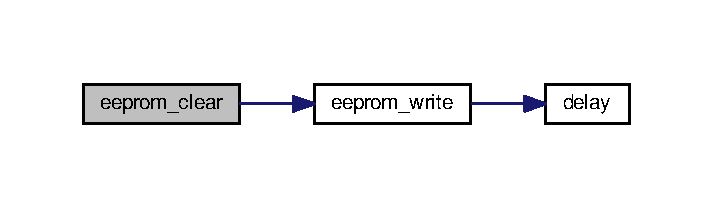
\includegraphics[width=342pt]{d2/de3/group___eeprom___trans_ga7964a5a66da1c4a59a42309a93752217_cgraph}
\end{center}
\end{figure}


\index{Transmission functions@{Transmission functions}!eeprom\+\_\+read@{eeprom\+\_\+read}}
\index{eeprom\+\_\+read@{eeprom\+\_\+read}!Transmission functions@{Transmission functions}}
\subsubsection[{\texorpdfstring{eeprom\+\_\+read(uint16\+\_\+t address)}{eeprom_read(uint16_t address)}}]{\setlength{\rightskip}{0pt plus 5cm}uint8\+\_\+t eeprom\+\_\+read (
\begin{DoxyParamCaption}
\item[{uint16\+\_\+t}]{address}
\end{DoxyParamCaption}
)}\hypertarget{group___eeprom___trans_gafaa7cca6f6ad1d9ae49522324c825c2f}{}\label{group___eeprom___trans_gafaa7cca6f6ad1d9ae49522324c825c2f}


Read a byte from the eeprom. 


\begin{DoxyParams}{Parameters}
{\em address} & The address of the memory \\
\hline
\end{DoxyParams}

\begin{DoxyRetVals}{Return values}
{\em uint8\+\_\+t} & data from eeprom \\
\hline
\end{DoxyRetVals}


Definition at line 156 of file N\+P\+C\+\_\+eeprom.\+c.



Here is the call graph for this function\+:\nopagebreak
\begin{figure}[H]
\begin{center}
\leavevmode
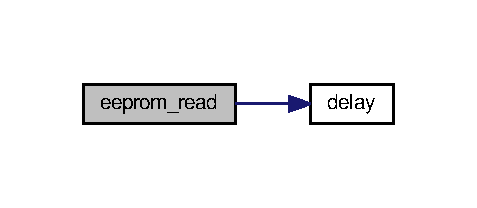
\includegraphics[width=229pt]{d2/de3/group___eeprom___trans_gafaa7cca6f6ad1d9ae49522324c825c2f_cgraph}
\end{center}
\end{figure}




Here is the caller graph for this function\+:
\nopagebreak
\begin{figure}[H]
\begin{center}
\leavevmode
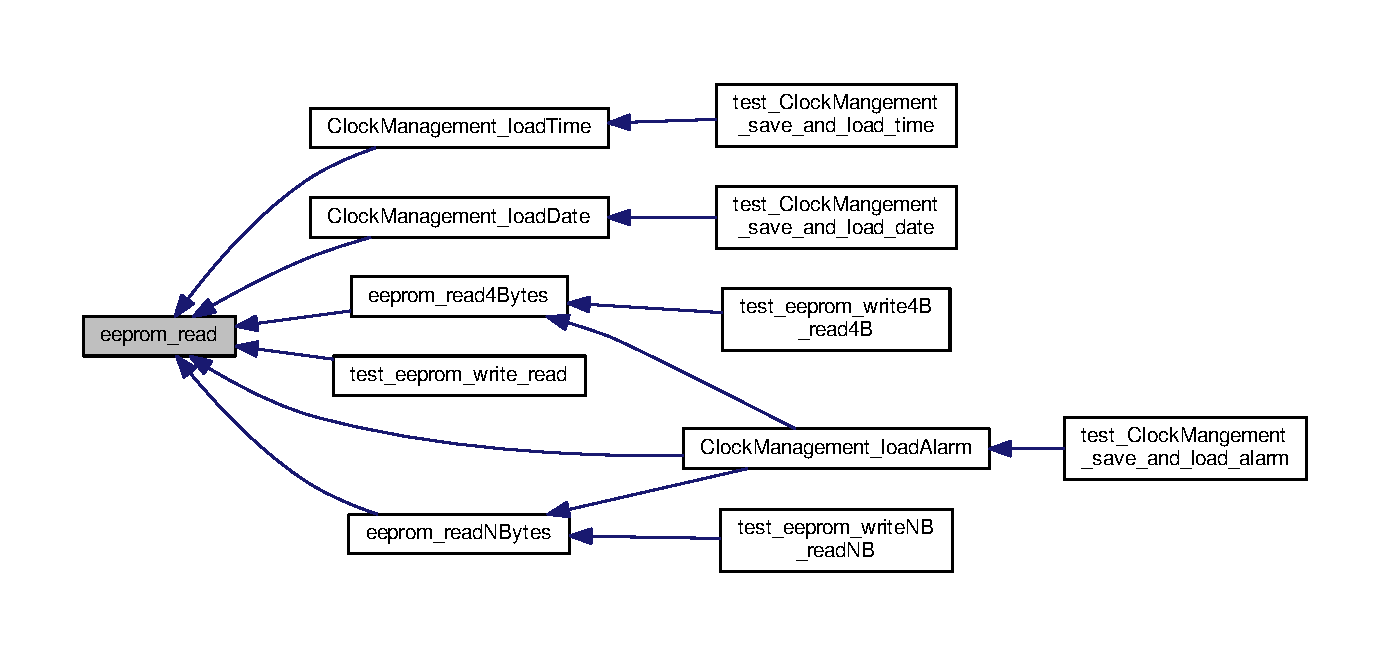
\includegraphics[width=350pt]{d2/de3/group___eeprom___trans_gafaa7cca6f6ad1d9ae49522324c825c2f_icgraph}
\end{center}
\end{figure}


\index{Transmission functions@{Transmission functions}!eeprom\+\_\+read4\+Bytes@{eeprom\+\_\+read4\+Bytes}}
\index{eeprom\+\_\+read4\+Bytes@{eeprom\+\_\+read4\+Bytes}!Transmission functions@{Transmission functions}}
\subsubsection[{\texorpdfstring{eeprom\+\_\+read4\+Bytes(uint16\+\_\+t base\+Address)}{eeprom_read4Bytes(uint16_t baseAddress)}}]{\setlength{\rightskip}{0pt plus 5cm}uint32\+\_\+t eeprom\+\_\+read4\+Bytes (
\begin{DoxyParamCaption}
\item[{uint16\+\_\+t}]{base\+Address}
\end{DoxyParamCaption}
)}\hypertarget{group___eeprom___trans_ga9a323370ddd02d91c6118f104c015b43}{}\label{group___eeprom___trans_ga9a323370ddd02d91c6118f104c015b43}


Read a 32byte from eeprom. 


\begin{DoxyParams}{Parameters}
{\em base\+Address} & \\
\hline
\end{DoxyParams}

\begin{DoxyRetVals}{Return values}
{\em uint32\+\_\+t} & \\
\hline
\end{DoxyRetVals}


Definition at line 295 of file N\+P\+C\+\_\+eeprom.\+c.



Here is the call graph for this function\+:\nopagebreak
\begin{figure}[H]
\begin{center}
\leavevmode
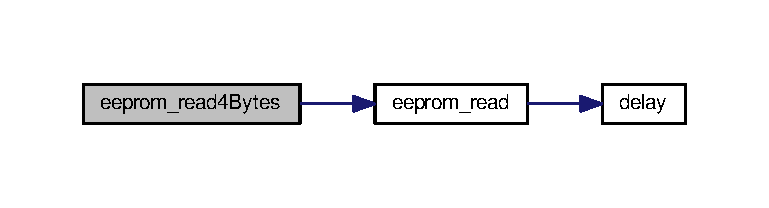
\includegraphics[width=350pt]{d2/de3/group___eeprom___trans_ga9a323370ddd02d91c6118f104c015b43_cgraph}
\end{center}
\end{figure}




Here is the caller graph for this function\+:\nopagebreak
\begin{figure}[H]
\begin{center}
\leavevmode
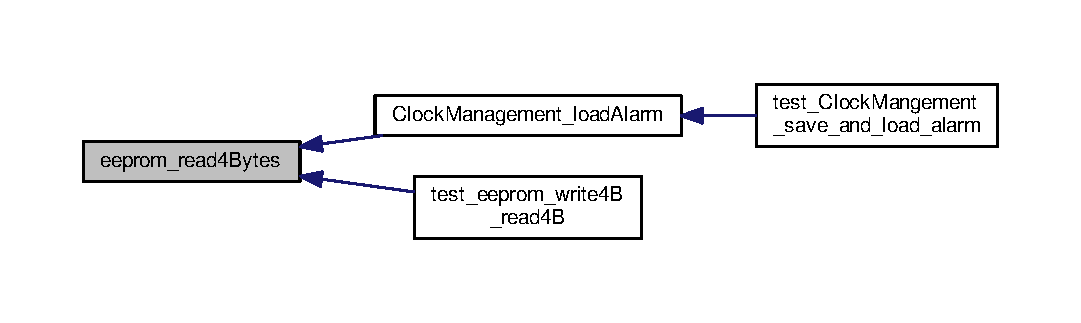
\includegraphics[width=350pt]{d2/de3/group___eeprom___trans_ga9a323370ddd02d91c6118f104c015b43_icgraph}
\end{center}
\end{figure}


\index{Transmission functions@{Transmission functions}!eeprom\+\_\+read\+N\+Bytes@{eeprom\+\_\+read\+N\+Bytes}}
\index{eeprom\+\_\+read\+N\+Bytes@{eeprom\+\_\+read\+N\+Bytes}!Transmission functions@{Transmission functions}}
\subsubsection[{\texorpdfstring{eeprom\+\_\+read\+N\+Bytes(uint16\+\_\+t base\+Address, uint8\+\_\+t $\ast$data, uint16\+\_\+t N)}{eeprom_readNBytes(uint16_t baseAddress, uint8_t *data, uint16_t N)}}]{\setlength{\rightskip}{0pt plus 5cm}void eeprom\+\_\+read\+N\+Bytes (
\begin{DoxyParamCaption}
\item[{uint16\+\_\+t}]{base\+Address, }
\item[{uint8\+\_\+t $\ast$}]{data, }
\item[{uint16\+\_\+t}]{N}
\end{DoxyParamCaption}
)}\hypertarget{group___eeprom___trans_gab7c6abb0e0c39a8c152307fb822ffa0c}{}\label{group___eeprom___trans_gab7c6abb0e0c39a8c152307fb822ffa0c}


Definition at line 309 of file N\+P\+C\+\_\+eeprom.\+c.



Here is the call graph for this function\+:
\nopagebreak
\begin{figure}[H]
\begin{center}
\leavevmode
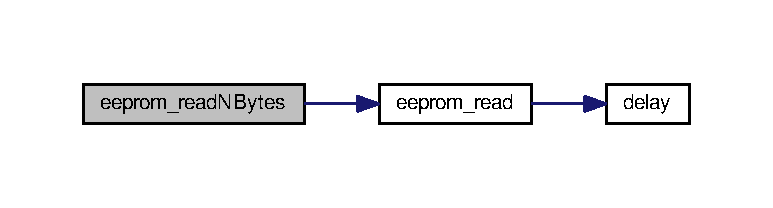
\includegraphics[width=350pt]{d2/de3/group___eeprom___trans_gab7c6abb0e0c39a8c152307fb822ffa0c_cgraph}
\end{center}
\end{figure}




Here is the caller graph for this function\+:
\nopagebreak
\begin{figure}[H]
\begin{center}
\leavevmode
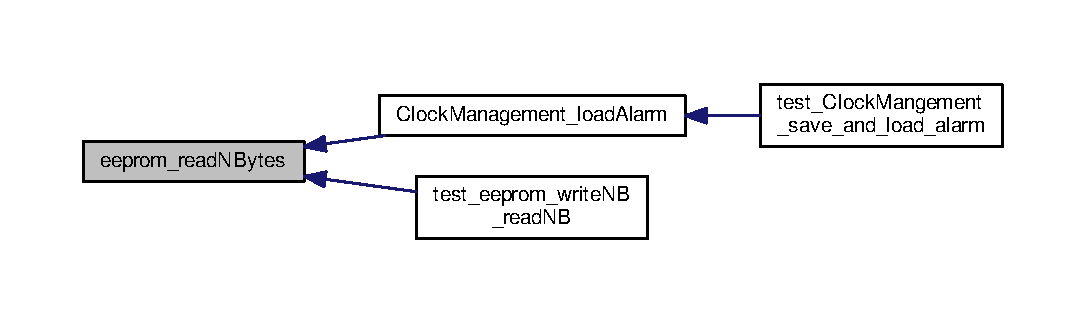
\includegraphics[width=350pt]{d2/de3/group___eeprom___trans_gab7c6abb0e0c39a8c152307fb822ffa0c_icgraph}
\end{center}
\end{figure}


\index{Transmission functions@{Transmission functions}!eeprom\+\_\+write@{eeprom\+\_\+write}}
\index{eeprom\+\_\+write@{eeprom\+\_\+write}!Transmission functions@{Transmission functions}}
\subsubsection[{\texorpdfstring{eeprom\+\_\+write(uint16\+\_\+t address, uint8\+\_\+t data)}{eeprom_write(uint16_t address, uint8_t data)}}]{\setlength{\rightskip}{0pt plus 5cm}Error\+Status eeprom\+\_\+write (
\begin{DoxyParamCaption}
\item[{uint16\+\_\+t}]{address, }
\item[{uint8\+\_\+t}]{data}
\end{DoxyParamCaption}
)}\hypertarget{group___eeprom___trans_ga46c7b6081a89f96d53b6ebc0d0b6f60b}{}\label{group___eeprom___trans_ga46c7b6081a89f96d53b6ebc0d0b6f60b}


Write a byte to the eeprom. 


\begin{DoxyParams}{Parameters}
{\em address} & The address of th memory \\
\hline
{\em data} & The data to be written to the memory \\
\hline
\end{DoxyParams}

\begin{DoxyRetVals}{Return values}
{\em None} & \\
\hline
\end{DoxyRetVals}


Definition at line 108 of file N\+P\+C\+\_\+eeprom.\+c.



Here is the call graph for this function\+:\nopagebreak
\begin{figure}[H]
\begin{center}
\leavevmode
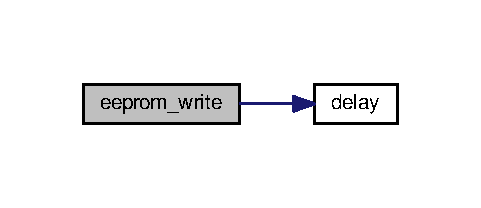
\includegraphics[width=231pt]{d2/de3/group___eeprom___trans_ga46c7b6081a89f96d53b6ebc0d0b6f60b_cgraph}
\end{center}
\end{figure}




Here is the caller graph for this function\+:
\nopagebreak
\begin{figure}[H]
\begin{center}
\leavevmode
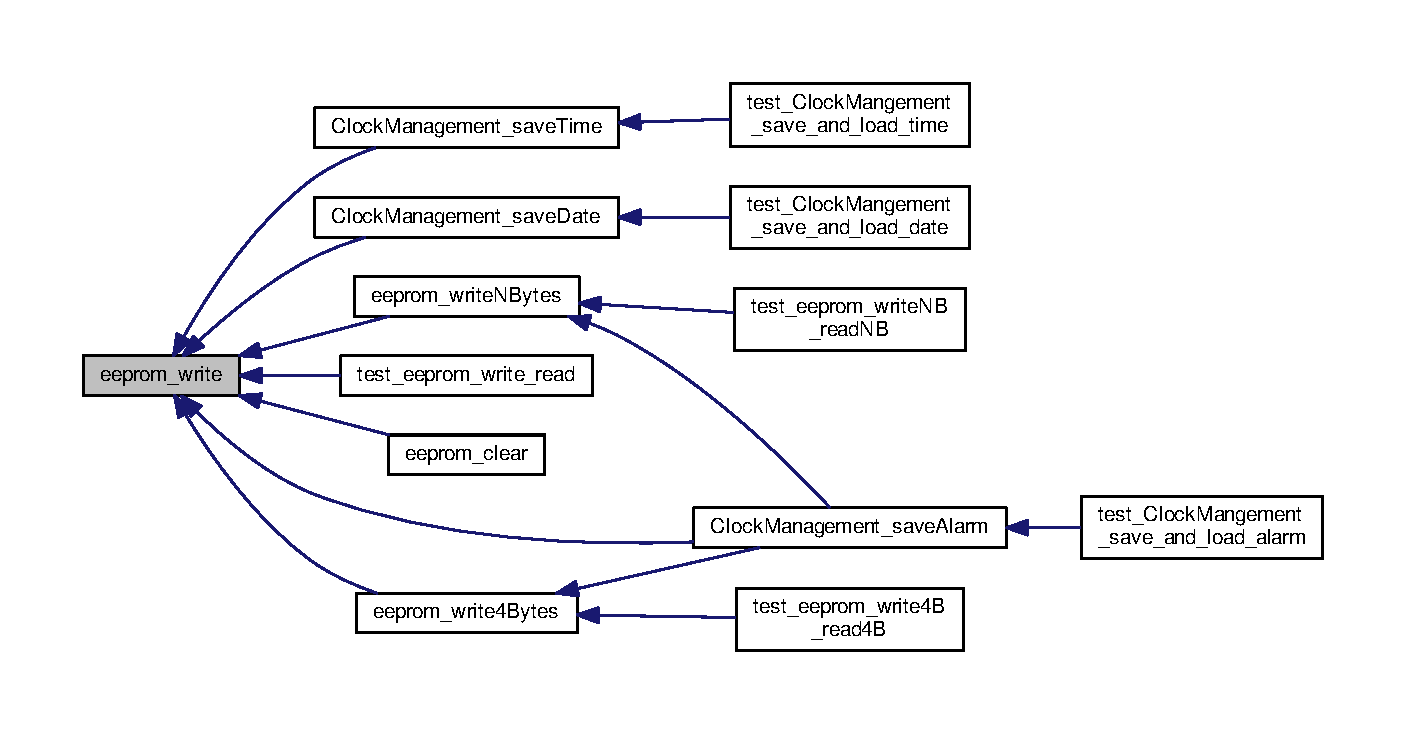
\includegraphics[width=350pt]{d2/de3/group___eeprom___trans_ga46c7b6081a89f96d53b6ebc0d0b6f60b_icgraph}
\end{center}
\end{figure}


\index{Transmission functions@{Transmission functions}!eeprom\+\_\+write32\+Bytes@{eeprom\+\_\+write32\+Bytes}}
\index{eeprom\+\_\+write32\+Bytes@{eeprom\+\_\+write32\+Bytes}!Transmission functions@{Transmission functions}}
\subsubsection[{\texorpdfstring{eeprom\+\_\+write32\+Bytes(uint16\+\_\+t base\+Address, uint8\+\_\+t $\ast$data)}{eeprom_write32Bytes(uint16_t baseAddress, uint8_t *data)}}]{\setlength{\rightskip}{0pt plus 5cm}Error\+Status eeprom\+\_\+write32\+Bytes (
\begin{DoxyParamCaption}
\item[{uint16\+\_\+t}]{base\+Address, }
\item[{uint8\+\_\+t $\ast$}]{data}
\end{DoxyParamCaption}
)}\hypertarget{group___eeprom___trans_ga8c4d6169df1fdb9baeca667b5e9b0058}{}\label{group___eeprom___trans_ga8c4d6169df1fdb9baeca667b5e9b0058}


Write a page to the eeprom. 


\begin{DoxyParams}{Parameters}
{\em base\+Address} & The base address of the page \\
\hline
{\em data} & An array of data to be send \\
\hline
\end{DoxyParams}

\begin{DoxyRetVals}{Return values}
{\em None} & \\
\hline
\end{DoxyRetVals}


Definition at line 192 of file N\+P\+C\+\_\+eeprom.\+c.



Here is the call graph for this function\+:\nopagebreak
\begin{figure}[H]
\begin{center}
\leavevmode
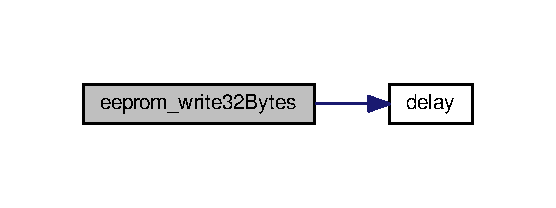
\includegraphics[width=267pt]{d2/de3/group___eeprom___trans_ga8c4d6169df1fdb9baeca667b5e9b0058_cgraph}
\end{center}
\end{figure}




Here is the caller graph for this function\+:\nopagebreak
\begin{figure}[H]
\begin{center}
\leavevmode
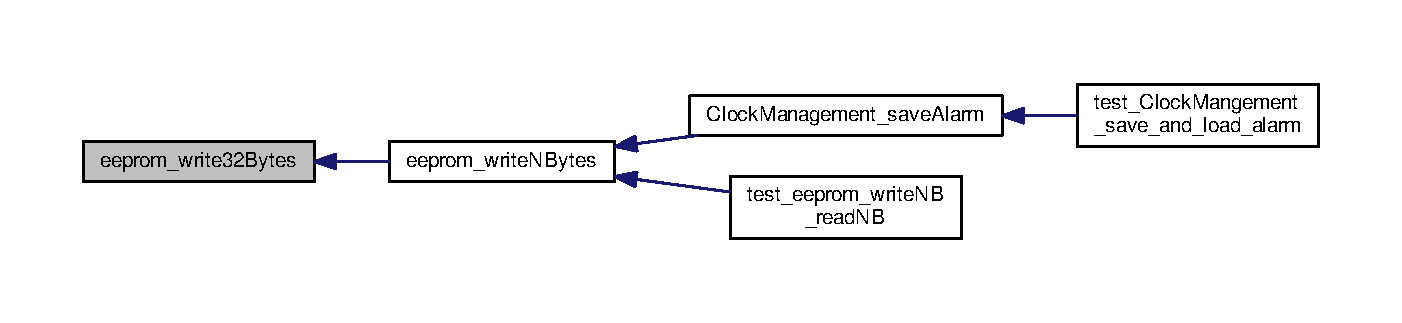
\includegraphics[width=350pt]{d2/de3/group___eeprom___trans_ga8c4d6169df1fdb9baeca667b5e9b0058_icgraph}
\end{center}
\end{figure}


\index{Transmission functions@{Transmission functions}!eeprom\+\_\+write4\+Bytes@{eeprom\+\_\+write4\+Bytes}}
\index{eeprom\+\_\+write4\+Bytes@{eeprom\+\_\+write4\+Bytes}!Transmission functions@{Transmission functions}}
\subsubsection[{\texorpdfstring{eeprom\+\_\+write4\+Bytes(uint16\+\_\+t base\+Address, uint8\+\_\+t $\ast$data)}{eeprom_write4Bytes(uint16_t baseAddress, uint8_t *data)}}]{\setlength{\rightskip}{0pt plus 5cm}Error\+Status eeprom\+\_\+write4\+Bytes (
\begin{DoxyParamCaption}
\item[{uint16\+\_\+t}]{base\+Address, }
\item[{uint8\+\_\+t $\ast$}]{data}
\end{DoxyParamCaption}
)}\hypertarget{group___eeprom___trans_ga7d9db4a4822fa0c3e5b811615aaed569}{}\label{group___eeprom___trans_ga7d9db4a4822fa0c3e5b811615aaed569}


Write 4 bytes to the eeprom. 


\begin{DoxyParams}{Parameters}
{\em base\+Address} & address of data \\
\hline
{\em data} & data to be written \\
\hline
\end{DoxyParams}

\begin{DoxyRetVals}{Return values}
{\em Error\+Status} & \\
\hline
\end{DoxyRetVals}


Definition at line 279 of file N\+P\+C\+\_\+eeprom.\+c.



Here is the call graph for this function\+:\nopagebreak
\begin{figure}[H]
\begin{center}
\leavevmode
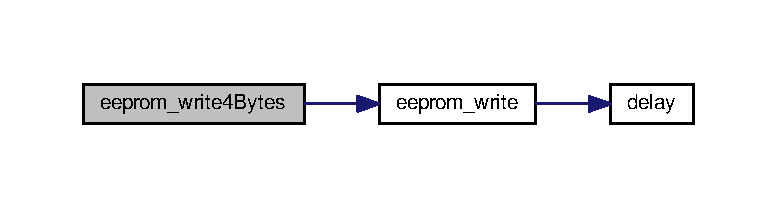
\includegraphics[width=350pt]{d2/de3/group___eeprom___trans_ga7d9db4a4822fa0c3e5b811615aaed569_cgraph}
\end{center}
\end{figure}




Here is the caller graph for this function\+:\nopagebreak
\begin{figure}[H]
\begin{center}
\leavevmode
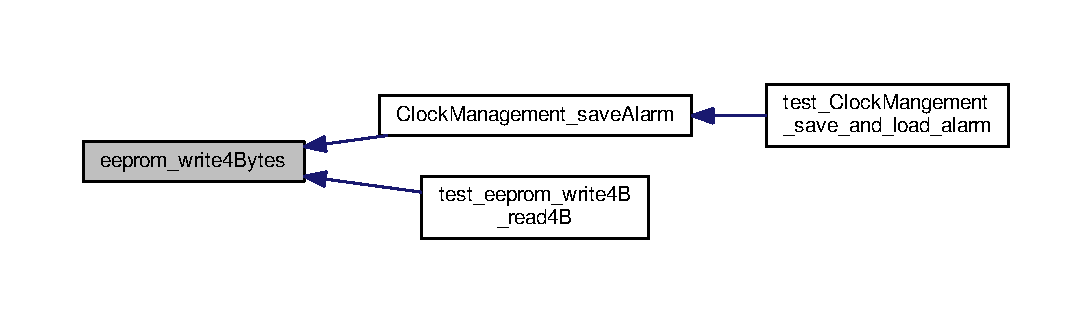
\includegraphics[width=350pt]{d2/de3/group___eeprom___trans_ga7d9db4a4822fa0c3e5b811615aaed569_icgraph}
\end{center}
\end{figure}


\index{Transmission functions@{Transmission functions}!eeprom\+\_\+write\+N\+Bytes@{eeprom\+\_\+write\+N\+Bytes}}
\index{eeprom\+\_\+write\+N\+Bytes@{eeprom\+\_\+write\+N\+Bytes}!Transmission functions@{Transmission functions}}
\subsubsection[{\texorpdfstring{eeprom\+\_\+write\+N\+Bytes(uint16\+\_\+t base\+Address, uint8\+\_\+t $\ast$data, uint16\+\_\+t N)}{eeprom_writeNBytes(uint16_t baseAddress, uint8_t *data, uint16_t N)}}]{\setlength{\rightskip}{0pt plus 5cm}Error\+Status eeprom\+\_\+write\+N\+Bytes (
\begin{DoxyParamCaption}
\item[{uint16\+\_\+t}]{base\+Address, }
\item[{uint8\+\_\+t $\ast$}]{data, }
\item[{uint16\+\_\+t}]{N}
\end{DoxyParamCaption}
)}\hypertarget{group___eeprom___trans_ga9dea9d824339ffc184a047749533b96d}{}\label{group___eeprom___trans_ga9dea9d824339ffc184a047749533b96d}


Write N bytes to the eeprom. 

\begin{DoxyNote}{Note}
N is divided into pages before been written to memory 
\end{DoxyNote}

\begin{DoxyParams}{Parameters}
{\em base\+Address} & address of data \\
\hline
{\em data} & data to be written \\
\hline
{\em N} & number of data to write \\
\hline
\end{DoxyParams}

\begin{DoxyRetVals}{Return values}
{\em Error\+Status} & \\
\hline
\end{DoxyRetVals}


Definition at line 259 of file N\+P\+C\+\_\+eeprom.\+c.



Here is the call graph for this function\+:\nopagebreak
\begin{figure}[H]
\begin{center}
\leavevmode
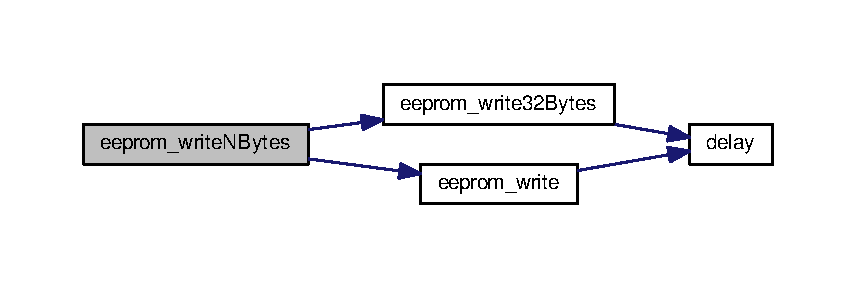
\includegraphics[width=350pt]{d2/de3/group___eeprom___trans_ga9dea9d824339ffc184a047749533b96d_cgraph}
\end{center}
\end{figure}




Here is the caller graph for this function\+:\nopagebreak
\begin{figure}[H]
\begin{center}
\leavevmode
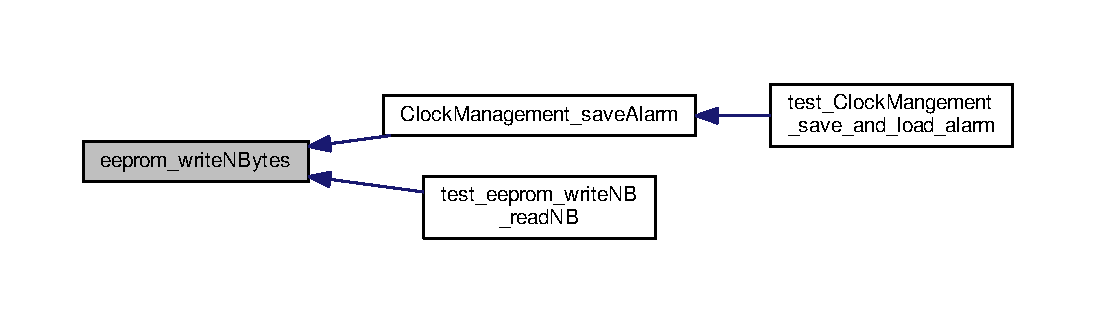
\includegraphics[width=350pt]{d2/de3/group___eeprom___trans_ga9dea9d824339ffc184a047749533b96d_icgraph}
\end{center}
\end{figure}



\hypertarget{group___neo_pixel___init}{}\section{Initialisation functions}
\label{group___neo_pixel___init}\index{Initialisation functions@{Initialisation functions}}


Neopixel initialisation functions.  


Collaboration diagram for Initialisation functions\+:
% FIG 0
\subsection*{Functions}
\begin{DoxyCompactItemize}
\item 
void \hyperlink{group___neo_pixel___init_gaac78468985e44a3e4d353ea9276b33bc}{neopixel\+\_\+init} (void)
\begin{DoxyCompactList}\small\item\em Initialise the neopixel. \end{DoxyCompactList}\end{DoxyCompactItemize}


\subsection{Detailed Description}
Neopixel initialisation functions. 



\subsection{Function Documentation}
\mbox{\Hypertarget{group___neo_pixel___init_gaac78468985e44a3e4d353ea9276b33bc}\label{group___neo_pixel___init_gaac78468985e44a3e4d353ea9276b33bc}} 
\index{Initialisation functions@{Initialisation functions}!neopixel\+\_\+init@{neopixel\+\_\+init}}
\index{neopixel\+\_\+init@{neopixel\+\_\+init}!Initialisation functions@{Initialisation functions}}
\subsubsection{\texorpdfstring{neopixel\+\_\+init()}{neopixel\_init()}}
{\footnotesize\ttfamily void neopixel\+\_\+init (\begin{DoxyParamCaption}\item[{void}]{ }\end{DoxyParamCaption})}



Initialise the neopixel. 


\begin{DoxyParams}{Parameters}
{\em None} & \\
\hline
\end{DoxyParams}

\begin{DoxyRetVals}{Return values}
{\em None} & \\
\hline
\end{DoxyRetVals}

\hypertarget{group___neo_pixel___state}{}\section{State alteration functions}
\label{group___neo_pixel___state}\index{State alteration functions@{State alteration functions}}


Neopixel state alteration functions.  


Collaboration diagram for State alteration functions\+:
% FIG 0
\subsection*{Functions}
\begin{DoxyCompactItemize}
\item 
void \hyperlink{group___neo_pixel___state_ga38ad4725462bdc5e86c4ead4f04b9fc2}{T\+I\+M2\+\_\+\+I\+R\+Q\+Handler} (void)
\begin{DoxyCompactList}\small\item\em Timer Handler for neopixel. \end{DoxyCompactList}\item 
void \hyperlink{group___neo_pixel___state_ga8e3cfef785ce221672f825f8785c25b8}{neopixel\+\_\+clear} (void)
\begin{DoxyCompactList}\small\item\em Stop pushing data to the neopixels. \end{DoxyCompactList}\item 
void \hyperlink{group___neo_pixel___state_ga79e34feddcfb2c45ae218166c84bdff4}{neopixel\+\_\+data\+Init} (void)
\begin{DoxyCompactList}\small\item\em Initialise the L\+E\+Dbuffer. \end{DoxyCompactList}\item 
void \hyperlink{group___neo_pixel___state_ga63c196a71ffb007411929e41ba5df41d}{neopixel\+\_\+set\+Pixel\+Colour\+R\+GB} (uint8\+\_\+t n, uint8\+\_\+t r, uint8\+\_\+t g, uint8\+\_\+t b)
\begin{DoxyCompactList}\small\item\em Set the colour of one led. \end{DoxyCompactList}\item 
void \hyperlink{group___neo_pixel___state_gae027558106eef5c81996294f4561fecb}{neopixel\+\_\+set\+Brightness} (uint8\+\_\+t b)
\begin{DoxyCompactList}\small\item\em Set the brightness of the led. \end{DoxyCompactList}\end{DoxyCompactItemize}


\subsection{Detailed Description}
Neopixel state alteration functions. 



\subsection{Function Documentation}
\mbox{\Hypertarget{group___neo_pixel___state_ga8e3cfef785ce221672f825f8785c25b8}\label{group___neo_pixel___state_ga8e3cfef785ce221672f825f8785c25b8}} 
\index{State alteration functions@{State alteration functions}!neopixel\+\_\+clear@{neopixel\+\_\+clear}}
\index{neopixel\+\_\+clear@{neopixel\+\_\+clear}!State alteration functions@{State alteration functions}}
\subsubsection{\texorpdfstring{neopixel\+\_\+clear()}{neopixel\_clear()}}
{\footnotesize\ttfamily void neopixel\+\_\+clear (\begin{DoxyParamCaption}\item[{void}]{ }\end{DoxyParamCaption})}



Stop pushing data to the neopixels. 


\begin{DoxyParams}{Parameters}
{\em None} & \\
\hline
\end{DoxyParams}

\begin{DoxyRetVals}{Return values}
{\em None} & \\
\hline
\end{DoxyRetVals}
\mbox{\Hypertarget{group___neo_pixel___state_ga79e34feddcfb2c45ae218166c84bdff4}\label{group___neo_pixel___state_ga79e34feddcfb2c45ae218166c84bdff4}} 
\index{State alteration functions@{State alteration functions}!neopixel\+\_\+data\+Init@{neopixel\+\_\+data\+Init}}
\index{neopixel\+\_\+data\+Init@{neopixel\+\_\+data\+Init}!State alteration functions@{State alteration functions}}
\subsubsection{\texorpdfstring{neopixel\+\_\+data\+Init()}{neopixel\_dataInit()}}
{\footnotesize\ttfamily void neopixel\+\_\+data\+Init (\begin{DoxyParamCaption}\item[{void}]{ }\end{DoxyParamCaption})}



Initialise the L\+E\+Dbuffer. 


\begin{DoxyParams}{Parameters}
{\em None} & \\
\hline
\end{DoxyParams}

\begin{DoxyRetVals}{Return values}
{\em None} & \\
\hline
\end{DoxyRetVals}
\mbox{\Hypertarget{group___neo_pixel___state_gae027558106eef5c81996294f4561fecb}\label{group___neo_pixel___state_gae027558106eef5c81996294f4561fecb}} 
\index{State alteration functions@{State alteration functions}!neopixel\+\_\+set\+Brightness@{neopixel\+\_\+set\+Brightness}}
\index{neopixel\+\_\+set\+Brightness@{neopixel\+\_\+set\+Brightness}!State alteration functions@{State alteration functions}}
\subsubsection{\texorpdfstring{neopixel\+\_\+set\+Brightness()}{neopixel\_setBrightness()}}
{\footnotesize\ttfamily void neopixel\+\_\+set\+Brightness (\begin{DoxyParamCaption}\item[{uint8\+\_\+t}]{b }\end{DoxyParamCaption})}



Set the brightness of the led. 

\begin{DoxyNote}{Note}
-\/ completely dim\+: 0
\begin{DoxyItemize}
\item fully bright\+: 255 
\end{DoxyItemize}
\end{DoxyNote}

\begin{DoxyParams}{Parameters}
{\em b} & Brightness \\
\hline
\end{DoxyParams}

\begin{DoxyRetVals}{Return values}
{\em None} & \\
\hline
\end{DoxyRetVals}
\mbox{\Hypertarget{group___neo_pixel___state_ga63c196a71ffb007411929e41ba5df41d}\label{group___neo_pixel___state_ga63c196a71ffb007411929e41ba5df41d}} 
\index{State alteration functions@{State alteration functions}!neopixel\+\_\+set\+Pixel\+Colour\+R\+GB@{neopixel\+\_\+set\+Pixel\+Colour\+R\+GB}}
\index{neopixel\+\_\+set\+Pixel\+Colour\+R\+GB@{neopixel\+\_\+set\+Pixel\+Colour\+R\+GB}!State alteration functions@{State alteration functions}}
\subsubsection{\texorpdfstring{neopixel\+\_\+set\+Pixel\+Colour\+R\+G\+B()}{neopixel\_setPixelColourRGB()}}
{\footnotesize\ttfamily void neopixel\+\_\+set\+Pixel\+Colour\+R\+GB (\begin{DoxyParamCaption}\item[{uint8\+\_\+t}]{n,  }\item[{uint8\+\_\+t}]{r,  }\item[{uint8\+\_\+t}]{g,  }\item[{uint8\+\_\+t}]{b }\end{DoxyParamCaption})}



Set the colour of one led. 


\begin{DoxyParams}{Parameters}
{\em n} & Led index \\
\hline
{\em r} & R\+ED intensity \\
\hline
{\em g} & G\+R\+E\+EN intensity \\
\hline
{\em b} & B\+L\+UE intensity \\
\hline
\end{DoxyParams}

\begin{DoxyRetVals}{Return values}
{\em None} & \\
\hline
\end{DoxyRetVals}
\mbox{\Hypertarget{group___neo_pixel___state_ga38ad4725462bdc5e86c4ead4f04b9fc2}\label{group___neo_pixel___state_ga38ad4725462bdc5e86c4ead4f04b9fc2}} 
\index{State alteration functions@{State alteration functions}!T\+I\+M2\+\_\+\+I\+R\+Q\+Handler@{T\+I\+M2\+\_\+\+I\+R\+Q\+Handler}}
\index{T\+I\+M2\+\_\+\+I\+R\+Q\+Handler@{T\+I\+M2\+\_\+\+I\+R\+Q\+Handler}!State alteration functions@{State alteration functions}}
\subsubsection{\texorpdfstring{T\+I\+M2\+\_\+\+I\+R\+Q\+Handler()}{TIM2\_IRQHandler()}}
{\footnotesize\ttfamily void T\+I\+M2\+\_\+\+I\+R\+Q\+Handler (\begin{DoxyParamCaption}\item[{void}]{ }\end{DoxyParamCaption})}



Timer Handler for neopixel. 

\begin{DoxyNote}{Note}
L\+E\+D\+Buffer is pushed every time the handle is called 
\end{DoxyNote}

\begin{DoxyParams}{Parameters}
{\em None} & \\
\hline
\end{DoxyParams}

\begin{DoxyRetVals}{Return values}
{\em None} & \\
\hline
\end{DoxyRetVals}

\hypertarget{group___neo_pixel___colour}{}\section{Colour generation functions}
\label{group___neo_pixel___colour}\index{Colour generation functions@{Colour generation functions}}


Neopixel colour functions.  


Collaboration diagram for Colour generation functions\+:
% FIG 0
\subsection*{Functions}
\begin{DoxyCompactItemize}
\item 
uint32\+\_\+t \hyperlink{group___neo_pixel___colour_ga1d500fbcbecad76feef8835437687ca0}{neopixel\+\_\+colour\+R\+GB} (uint8\+\_\+t r, uint8\+\_\+t g, uint8\+\_\+t b)
\begin{DoxyCompactList}\small\item\em convert R\+GB 3 8bit colour to a 32bit colour \end{DoxyCompactList}\item 
uint32\+\_\+t \hyperlink{group___neo_pixel___colour_ga527ba03b45a249e5e1ea1da4b971b3ac}{neopixel\+\_\+colour\+R\+G\+BW} (uint8\+\_\+t r, uint8\+\_\+t g, uint8\+\_\+t b, uint8\+\_\+t w)
\begin{DoxyCompactList}\small\item\em convert R\+GB 3 8bit colour to a 32bit colour \end{DoxyCompactList}\end{DoxyCompactItemize}


\subsection{Detailed Description}
Neopixel colour functions. 



\subsection{Function Documentation}
\mbox{\Hypertarget{group___neo_pixel___colour_ga1d500fbcbecad76feef8835437687ca0}\label{group___neo_pixel___colour_ga1d500fbcbecad76feef8835437687ca0}} 
\index{Colour generation functions@{Colour generation functions}!neopixel\+\_\+colour\+R\+GB@{neopixel\+\_\+colour\+R\+GB}}
\index{neopixel\+\_\+colour\+R\+GB@{neopixel\+\_\+colour\+R\+GB}!Colour generation functions@{Colour generation functions}}
\subsubsection{\texorpdfstring{neopixel\+\_\+colour\+R\+G\+B()}{neopixel\_colourRGB()}}
{\footnotesize\ttfamily uint32\+\_\+t neopixel\+\_\+colour\+R\+GB (\begin{DoxyParamCaption}\item[{uint8\+\_\+t}]{r,  }\item[{uint8\+\_\+t}]{g,  }\item[{uint8\+\_\+t}]{b }\end{DoxyParamCaption})}



convert R\+GB 3 8bit colour to a 32bit colour 

\begin{DoxyNote}{Note}
M\+S3 0, M\+S2 r, M\+S1 g, M\+S0 b 
\end{DoxyNote}

\begin{DoxyParams}{Parameters}
{\em r} & R\+ED intensity \\
\hline
{\em g} & G\+R\+E\+EN intensity \\
\hline
{\em b} & B\+L\+UE intensity \\
\hline
\end{DoxyParams}

\begin{DoxyRetVals}{Return values}
{\em None} & \\
\hline
\end{DoxyRetVals}
\mbox{\Hypertarget{group___neo_pixel___colour_ga527ba03b45a249e5e1ea1da4b971b3ac}\label{group___neo_pixel___colour_ga527ba03b45a249e5e1ea1da4b971b3ac}} 
\index{Colour generation functions@{Colour generation functions}!neopixel\+\_\+colour\+R\+G\+BW@{neopixel\+\_\+colour\+R\+G\+BW}}
\index{neopixel\+\_\+colour\+R\+G\+BW@{neopixel\+\_\+colour\+R\+G\+BW}!Colour generation functions@{Colour generation functions}}
\subsubsection{\texorpdfstring{neopixel\+\_\+colour\+R\+G\+B\+W()}{neopixel\_colourRGBW()}}
{\footnotesize\ttfamily uint32\+\_\+t neopixel\+\_\+colour\+R\+G\+BW (\begin{DoxyParamCaption}\item[{uint8\+\_\+t}]{r,  }\item[{uint8\+\_\+t}]{g,  }\item[{uint8\+\_\+t}]{b,  }\item[{uint8\+\_\+t}]{w }\end{DoxyParamCaption})}



convert R\+GB 3 8bit colour to a 32bit colour 

\begin{DoxyNote}{Note}
M\+S3 w, M\+S2 r, M\+S1 g, M\+S0 b 
\end{DoxyNote}

\begin{DoxyParams}{Parameters}
{\em r} & R\+ED intensity \\
\hline
{\em g} & G\+R\+E\+EN intensity \\
\hline
{\em b} & B\+L\+UE intensity \\
\hline
{\em w} & W\+H\+I\+TE intensity \\
\hline
\end{DoxyParams}

\begin{DoxyRetVals}{Return values}
{\em None} & \\
\hline
\end{DoxyRetVals}

\hypertarget{group___neo_pixel___display}{}\section{colour display functions}
\label{group___neo_pixel___display}\index{colour display functions@{colour display functions}}


Neopixel colour display functions.  


Collaboration diagram for colour display functions\+:
% FIG 0
\subsection*{Functions}
\begin{DoxyCompactItemize}
\item 
void \hyperlink{group___neo_pixel___display_ga58d5ceb79029ca8dc5dd8b27b65e4f09}{neopixel\+\_\+set\+Pixel\+Colour\+R\+G\+BW} (uint8\+\_\+t n, uint8\+\_\+t r, uint8\+\_\+t g, uint8\+\_\+t b, uint8\+\_\+t w)
\begin{DoxyCompactList}\small\item\em Set the colour of one led. \end{DoxyCompactList}\item 
void \hyperlink{group___neo_pixel___display_gaecbdecac1da356c5fba07058983d9066}{neopixel\+\_\+set\+Pixel\+Colour} (uint8\+\_\+t n, uint32\+\_\+t c)
\begin{DoxyCompactList}\small\item\em Set the colour of one led. \end{DoxyCompactList}\item 
void \hyperlink{group___neo_pixel___display_ga4daf6edfe83394f425ec51f64d92c49c}{neopixel\+\_\+set\+Pixel\+ColourW} (uint8\+\_\+t n, uint32\+\_\+t c)
\begin{DoxyCompactList}\small\item\em Set the colour of one led. \end{DoxyCompactList}\item 
void \hyperlink{group___neo_pixel___display_ga7a6c2dc149e86a788aede1d6aa5262d7}{neopixel\+\_\+set\+All\+Pixel\+R\+GB} (uint8\+\_\+t r, uint8\+\_\+t g, uint8\+\_\+t b)
\begin{DoxyCompactList}\small\item\em set all the pixel on the line to a specific colour \end{DoxyCompactList}\item 
void \hyperlink{group___neo_pixel___display_ga1ba017c1f338ef2c8e4a48acae35d87e}{neopixel\+\_\+set\+All\+Pixel\+R\+G\+BW} (uint8\+\_\+t r, uint8\+\_\+t g, uint8\+\_\+t b, uint8\+\_\+t w)
\begin{DoxyCompactList}\small\item\em set all the pixel on the line to a specific colour \end{DoxyCompactList}\end{DoxyCompactItemize}


\subsection{Detailed Description}
Neopixel colour display functions. 



\subsection{Function Documentation}
\mbox{\Hypertarget{group___neo_pixel___display_ga7a6c2dc149e86a788aede1d6aa5262d7}\label{group___neo_pixel___display_ga7a6c2dc149e86a788aede1d6aa5262d7}} 
\index{colour display functions@{colour display functions}!neopixel\+\_\+set\+All\+Pixel\+R\+GB@{neopixel\+\_\+set\+All\+Pixel\+R\+GB}}
\index{neopixel\+\_\+set\+All\+Pixel\+R\+GB@{neopixel\+\_\+set\+All\+Pixel\+R\+GB}!colour display functions@{colour display functions}}
\subsubsection{\texorpdfstring{neopixel\+\_\+set\+All\+Pixel\+R\+G\+B()}{neopixel\_setAllPixelRGB()}}
{\footnotesize\ttfamily void neopixel\+\_\+set\+All\+Pixel\+R\+GB (\begin{DoxyParamCaption}\item[{uint8\+\_\+t}]{r,  }\item[{uint8\+\_\+t}]{g,  }\item[{uint8\+\_\+t}]{b }\end{DoxyParamCaption})}



set all the pixel on the line to a specific colour 


\begin{DoxyParams}{Parameters}
{\em r} & R\+ED intensity \\
\hline
{\em g} & G\+R\+E\+EN intensity \\
\hline
{\em b} & B\+L\+UE intensity \\
\hline
\end{DoxyParams}

\begin{DoxyRetVals}{Return values}
{\em None} & \\
\hline
\end{DoxyRetVals}
\mbox{\Hypertarget{group___neo_pixel___display_ga1ba017c1f338ef2c8e4a48acae35d87e}\label{group___neo_pixel___display_ga1ba017c1f338ef2c8e4a48acae35d87e}} 
\index{colour display functions@{colour display functions}!neopixel\+\_\+set\+All\+Pixel\+R\+G\+BW@{neopixel\+\_\+set\+All\+Pixel\+R\+G\+BW}}
\index{neopixel\+\_\+set\+All\+Pixel\+R\+G\+BW@{neopixel\+\_\+set\+All\+Pixel\+R\+G\+BW}!colour display functions@{colour display functions}}
\subsubsection{\texorpdfstring{neopixel\+\_\+set\+All\+Pixel\+R\+G\+B\+W()}{neopixel\_setAllPixelRGBW()}}
{\footnotesize\ttfamily void neopixel\+\_\+set\+All\+Pixel\+R\+G\+BW (\begin{DoxyParamCaption}\item[{uint8\+\_\+t}]{r,  }\item[{uint8\+\_\+t}]{g,  }\item[{uint8\+\_\+t}]{b,  }\item[{uint8\+\_\+t}]{w }\end{DoxyParamCaption})}



set all the pixel on the line to a specific colour 


\begin{DoxyParams}{Parameters}
{\em r} & R\+ED intensity \\
\hline
{\em g} & G\+R\+E\+EN intensity \\
\hline
{\em b} & B\+L\+UE intensity \\
\hline
{\em w} & W\+H\+I\+TE intensity \\
\hline
\end{DoxyParams}

\begin{DoxyRetVals}{Return values}
{\em None} & \\
\hline
\end{DoxyRetVals}
\mbox{\Hypertarget{group___neo_pixel___display_gaecbdecac1da356c5fba07058983d9066}\label{group___neo_pixel___display_gaecbdecac1da356c5fba07058983d9066}} 
\index{colour display functions@{colour display functions}!neopixel\+\_\+set\+Pixel\+Colour@{neopixel\+\_\+set\+Pixel\+Colour}}
\index{neopixel\+\_\+set\+Pixel\+Colour@{neopixel\+\_\+set\+Pixel\+Colour}!colour display functions@{colour display functions}}
\subsubsection{\texorpdfstring{neopixel\+\_\+set\+Pixel\+Colour()}{neopixel\_setPixelColour()}}
{\footnotesize\ttfamily void neopixel\+\_\+set\+Pixel\+Colour (\begin{DoxyParamCaption}\item[{uint8\+\_\+t}]{n,  }\item[{uint32\+\_\+t}]{c }\end{DoxyParamCaption})}



Set the colour of one led. 


\begin{DoxyParams}{Parameters}
{\em n} & Led index \\
\hline
{\em c} & 32bit R\+GB colour \\
\hline
\end{DoxyParams}

\begin{DoxyRetVals}{Return values}
{\em None} & \\
\hline
\end{DoxyRetVals}
\mbox{\Hypertarget{group___neo_pixel___display_ga58d5ceb79029ca8dc5dd8b27b65e4f09}\label{group___neo_pixel___display_ga58d5ceb79029ca8dc5dd8b27b65e4f09}} 
\index{colour display functions@{colour display functions}!neopixel\+\_\+set\+Pixel\+Colour\+R\+G\+BW@{neopixel\+\_\+set\+Pixel\+Colour\+R\+G\+BW}}
\index{neopixel\+\_\+set\+Pixel\+Colour\+R\+G\+BW@{neopixel\+\_\+set\+Pixel\+Colour\+R\+G\+BW}!colour display functions@{colour display functions}}
\subsubsection{\texorpdfstring{neopixel\+\_\+set\+Pixel\+Colour\+R\+G\+B\+W()}{neopixel\_setPixelColourRGBW()}}
{\footnotesize\ttfamily void neopixel\+\_\+set\+Pixel\+Colour\+R\+G\+BW (\begin{DoxyParamCaption}\item[{uint8\+\_\+t}]{n,  }\item[{uint8\+\_\+t}]{r,  }\item[{uint8\+\_\+t}]{g,  }\item[{uint8\+\_\+t}]{b,  }\item[{uint8\+\_\+t}]{w }\end{DoxyParamCaption})}



Set the colour of one led. 


\begin{DoxyParams}{Parameters}
{\em n} & Led index \\
\hline
{\em r} & R\+ED intensity \\
\hline
{\em g} & G\+R\+E\+EN intensity \\
\hline
{\em b} & B\+L\+UE intensity \\
\hline
{\em w} & W\+H\+I\+TE intensity \\
\hline
\end{DoxyParams}

\begin{DoxyRetVals}{Return values}
{\em None} & \\
\hline
\end{DoxyRetVals}
\mbox{\Hypertarget{group___neo_pixel___display_ga4daf6edfe83394f425ec51f64d92c49c}\label{group___neo_pixel___display_ga4daf6edfe83394f425ec51f64d92c49c}} 
\index{colour display functions@{colour display functions}!neopixel\+\_\+set\+Pixel\+ColourW@{neopixel\+\_\+set\+Pixel\+ColourW}}
\index{neopixel\+\_\+set\+Pixel\+ColourW@{neopixel\+\_\+set\+Pixel\+ColourW}!colour display functions@{colour display functions}}
\subsubsection{\texorpdfstring{neopixel\+\_\+set\+Pixel\+Colour\+W()}{neopixel\_setPixelColourW()}}
{\footnotesize\ttfamily void neopixel\+\_\+set\+Pixel\+ColourW (\begin{DoxyParamCaption}\item[{uint8\+\_\+t}]{n,  }\item[{uint32\+\_\+t}]{c }\end{DoxyParamCaption})}



Set the colour of one led. 


\begin{DoxyParams}{Parameters}
{\em n} & Led index \\
\hline
{\em c} & 32bit R\+GB colour \\
\hline
\end{DoxyParams}

\begin{DoxyRetVals}{Return values}
{\em None} & \\
\hline
\end{DoxyRetVals}

\hypertarget{group___temperature___init}{}\section{Initialise the temperature reader}
\label{group___temperature___init}\index{Initialise the temperature reader@{Initialise the temperature reader}}
Collaboration diagram for Initialise the temperature reader\+:
% FIG 0
\subsection*{Functions}
\begin{DoxyCompactItemize}
\item 
void \hyperlink{group___temperature___init_ga7da890f6748bbeb05511fd20100cb6ef}{temperature\+\_\+init} (void)
\begin{DoxyCompactList}\small\item\em Initialise the A\+DC. \end{DoxyCompactList}\end{DoxyCompactItemize}


\subsection{Detailed Description}


\subsection{Function Documentation}
\mbox{\Hypertarget{group___temperature___init_ga7da890f6748bbeb05511fd20100cb6ef}\label{group___temperature___init_ga7da890f6748bbeb05511fd20100cb6ef}} 
\index{Initialise the temperature reader@{Initialise the temperature reader}!temperature\+\_\+init@{temperature\+\_\+init}}
\index{temperature\+\_\+init@{temperature\+\_\+init}!Initialise the temperature reader@{Initialise the temperature reader}}
\subsubsection{\texorpdfstring{temperature\+\_\+init()}{temperature\_init()}}
{\footnotesize\ttfamily void temperature\+\_\+init (\begin{DoxyParamCaption}\item[{void}]{ }\end{DoxyParamCaption})}



Initialise the A\+DC. 

\begin{DoxyNote}{Note}
This function configure the A\+DC peripheral 1) Enable peripheral clocks 3) Configure A\+DC channel8 pin as analog input 4) Configure A\+D\+C1 channel 1 
\end{DoxyNote}

\begin{DoxyParams}{Parameters}
{\em None} & \\
\hline
\end{DoxyParams}

\begin{DoxyRetVals}{Return values}
{\em None} & \\
\hline
\end{DoxyRetVals}

\hypertarget{group___temperature___data}{}\section{Temperature information}
\label{group___temperature___data}\index{Temperature information@{Temperature information}}
\subsection*{Functions}
\begin{DoxyCompactItemize}
\item 
uint16\+\_\+t \hyperlink{group___temperature___data_ga74915aedf88ee7840a64ab372d768ca1}{temperature\+\_\+value} (void)
\begin{DoxyCompactList}\small\item\em Read A\+DC value. \end{DoxyCompactList}\item 
int32\+\_\+t \hyperlink{group___temperature___data_gad2e261b9f6af30d5857f1e2a892a9592}{temperature\+\_\+read} (void)
\begin{DoxyCompactList}\small\item\em Convert the A\+DC value to its corresponding temperature value. \end{DoxyCompactList}\end{DoxyCompactItemize}


\subsection{Detailed Description}


\subsection{Function Documentation}
\mbox{\Hypertarget{group___temperature___data_gad2e261b9f6af30d5857f1e2a892a9592}\label{group___temperature___data_gad2e261b9f6af30d5857f1e2a892a9592}} 
\index{Temperature information@{Temperature information}!temperature\+\_\+read@{temperature\+\_\+read}}
\index{temperature\+\_\+read@{temperature\+\_\+read}!Temperature information@{Temperature information}}
\subsubsection{\texorpdfstring{temperature\+\_\+read()}{temperature\_read()}}
{\footnotesize\ttfamily int32\+\_\+t temperature\+\_\+read (\begin{DoxyParamCaption}\item[{void}]{ }\end{DoxyParamCaption})}



Convert the A\+DC value to its corresponding temperature value. 


\begin{DoxyParams}{Parameters}
{\em None} & \\
\hline
\end{DoxyParams}

\begin{DoxyRetVals}{Return values}
{\em int32\+\_\+t} & of the temperature read \\
\hline
\end{DoxyRetVals}
\mbox{\Hypertarget{group___temperature___data_ga74915aedf88ee7840a64ab372d768ca1}\label{group___temperature___data_ga74915aedf88ee7840a64ab372d768ca1}} 
\index{Temperature information@{Temperature information}!temperature\+\_\+value@{temperature\+\_\+value}}
\index{temperature\+\_\+value@{temperature\+\_\+value}!Temperature information@{Temperature information}}
\subsubsection{\texorpdfstring{temperature\+\_\+value()}{temperature\_value()}}
{\footnotesize\ttfamily uint16\+\_\+t temperature\+\_\+value (\begin{DoxyParamCaption}\item[{void}]{ }\end{DoxyParamCaption})}



Read A\+DC value. 


\begin{DoxyParams}{Parameters}
{\em None} & \\
\hline
\end{DoxyParams}

\begin{DoxyRetVals}{Return values}
{\em uint32\+\_\+t} & of the A\+DC value \\
\hline
\end{DoxyRetVals}

\hypertarget{group__nextion___constants}{}\section{Nextion\+\_\+\+Constants}
\label{group__nextion___constants}\index{Nextion\+\_\+\+Constants@{Nextion\+\_\+\+Constants}}


define nextion constant  


Collaboration diagram for Nextion\+\_\+\+Constants\+:\nopagebreak
\begin{figure}[H]
\begin{center}
\leavevmode
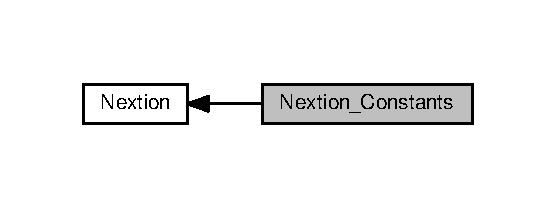
\includegraphics[width=267pt]{d8/d87/group__nextion___constants}
\end{center}
\end{figure}
\subsection*{Macros}
\begin{DoxyCompactItemize}
\item 
\#define \hyperlink{group__nextion___constants_ga523f9520cea00f41b66c2b01fc0865e6}{N\+E\+X\+T\+I\+O\+N\+\_\+\+P\+E\+R\+I\+P\+H\+\_\+\+U\+S\+A\+R\+TX}~R\+C\+C\+\_\+\+A\+P\+B1\+Periph\+\_\+\+U\+S\+A\+R\+T2
\item 
\#define \hyperlink{group__nextion___constants_ga0196543a58aaa665478912e81c89d98a}{N\+E\+X\+T\+I\+O\+N\+\_\+\+P\+E\+R\+I\+P\+H\+\_\+\+G\+P\+I\+OX}~R\+C\+C\+\_\+\+A\+H\+B1\+Periph\+\_\+\+G\+P\+I\+OA
\item 
\#define \hyperlink{group__nextion___constants_gab6c406ec72b8a3e97f1808c45b638af0}{N\+E\+X\+T\+I\+O\+N\+\_\+\+G\+P\+I\+OX}~G\+P\+I\+OA
\item 
\#define \hyperlink{group__nextion___constants_gaa79fddaf825d5ea9b2da1c513cf7f33c}{N\+E\+X\+T\+I\+O\+N\+\_\+\+T\+X\+\_\+\+P\+IN}~G\+P\+I\+O\+\_\+\+Pin\+\_\+2
\item 
\#define \hyperlink{group__nextion___constants_ga0b9b07a73114a9307ebbeb77b8c47197}{N\+E\+X\+T\+I\+O\+N\+\_\+\+R\+X\+\_\+\+P\+IN}~G\+P\+I\+O\+\_\+\+Pin\+\_\+3
\item 
\#define \hyperlink{group__nextion___constants_gafefb806155aed3ab1f0d24fb6354013d}{N\+E\+X\+T\+I\+O\+N\+\_\+\+T\+X\+\_\+\+P\+I\+N\+S\+O\+U\+R\+CE}~G\+P\+I\+O\+\_\+\+Pin\+Source2
\item 
\#define \hyperlink{group__nextion___constants_gaf726552562001a24196beeebbda67b0e}{N\+E\+X\+T\+I\+O\+N\+\_\+\+R\+X\+\_\+\+P\+I\+N\+S\+O\+U\+R\+CE}~G\+P\+I\+O\+\_\+\+Pin\+Source3
\item 
\#define \hyperlink{group__nextion___constants_ga7ed41bc717c1e697ef0d66f1a385c3e9}{N\+E\+X\+T\+I\+O\+N\+\_\+\+A\+F\+\_\+\+U\+S\+A\+RT}~G\+P\+I\+O\+\_\+\+A\+F\+\_\+\+U\+S\+A\+R\+T2
\item 
\#define \hyperlink{group__nextion___constants_gad110200ed1c63345918573270b4666ee}{N\+E\+X\+T\+I\+O\+N\+\_\+\+U\+S\+A\+R\+TX}~U\+S\+A\+R\+T2
\item 
\#define \hyperlink{group__nextion___constants_ga781191cedaf0e3bbbe8e3a37d54a7d2c}{N\+E\+X\+T\+I\+O\+N\+\_\+\+U\+S\+A\+R\+T\+X\+\_\+\+I\+RQ}~U\+S\+A\+R\+T2\+\_\+\+I\+R\+Qn
\item 
\#define \hyperlink{group__nextion___constants_gaf4e8e457f0055ebab4c1bf8a04d6473e}{N\+E\+X\+T\+I\+O\+N\+\_\+\+B\+A\+U\+D\+R\+A\+TE}~9600
\end{DoxyCompactItemize}


\subsection{Detailed Description}
define nextion constant 



\subsection{Macro Definition Documentation}
\index{Nextion\+\_\+\+Constants@{Nextion\+\_\+\+Constants}!N\+E\+X\+T\+I\+O\+N\+\_\+\+A\+F\+\_\+\+U\+S\+A\+RT@{N\+E\+X\+T\+I\+O\+N\+\_\+\+A\+F\+\_\+\+U\+S\+A\+RT}}
\index{N\+E\+X\+T\+I\+O\+N\+\_\+\+A\+F\+\_\+\+U\+S\+A\+RT@{N\+E\+X\+T\+I\+O\+N\+\_\+\+A\+F\+\_\+\+U\+S\+A\+RT}!Nextion\+\_\+\+Constants@{Nextion\+\_\+\+Constants}}
\subsubsection[{\texorpdfstring{N\+E\+X\+T\+I\+O\+N\+\_\+\+A\+F\+\_\+\+U\+S\+A\+RT}{NEXTION_AF_USART}}]{\setlength{\rightskip}{0pt plus 5cm}\#define N\+E\+X\+T\+I\+O\+N\+\_\+\+A\+F\+\_\+\+U\+S\+A\+RT~G\+P\+I\+O\+\_\+\+A\+F\+\_\+\+U\+S\+A\+R\+T2}\hypertarget{group__nextion___constants_ga7ed41bc717c1e697ef0d66f1a385c3e9}{}\label{group__nextion___constants_ga7ed41bc717c1e697ef0d66f1a385c3e9}


Definition at line 48 of file N\+P\+S\+C\+\_\+nextion.\+h.

\index{Nextion\+\_\+\+Constants@{Nextion\+\_\+\+Constants}!N\+E\+X\+T\+I\+O\+N\+\_\+\+B\+A\+U\+D\+R\+A\+TE@{N\+E\+X\+T\+I\+O\+N\+\_\+\+B\+A\+U\+D\+R\+A\+TE}}
\index{N\+E\+X\+T\+I\+O\+N\+\_\+\+B\+A\+U\+D\+R\+A\+TE@{N\+E\+X\+T\+I\+O\+N\+\_\+\+B\+A\+U\+D\+R\+A\+TE}!Nextion\+\_\+\+Constants@{Nextion\+\_\+\+Constants}}
\subsubsection[{\texorpdfstring{N\+E\+X\+T\+I\+O\+N\+\_\+\+B\+A\+U\+D\+R\+A\+TE}{NEXTION_BAUDRATE}}]{\setlength{\rightskip}{0pt plus 5cm}\#define N\+E\+X\+T\+I\+O\+N\+\_\+\+B\+A\+U\+D\+R\+A\+TE~9600}\hypertarget{group__nextion___constants_gaf4e8e457f0055ebab4c1bf8a04d6473e}{}\label{group__nextion___constants_gaf4e8e457f0055ebab4c1bf8a04d6473e}


Definition at line 51 of file N\+P\+S\+C\+\_\+nextion.\+h.

\index{Nextion\+\_\+\+Constants@{Nextion\+\_\+\+Constants}!N\+E\+X\+T\+I\+O\+N\+\_\+\+G\+P\+I\+OX@{N\+E\+X\+T\+I\+O\+N\+\_\+\+G\+P\+I\+OX}}
\index{N\+E\+X\+T\+I\+O\+N\+\_\+\+G\+P\+I\+OX@{N\+E\+X\+T\+I\+O\+N\+\_\+\+G\+P\+I\+OX}!Nextion\+\_\+\+Constants@{Nextion\+\_\+\+Constants}}
\subsubsection[{\texorpdfstring{N\+E\+X\+T\+I\+O\+N\+\_\+\+G\+P\+I\+OX}{NEXTION_GPIOX}}]{\setlength{\rightskip}{0pt plus 5cm}\#define N\+E\+X\+T\+I\+O\+N\+\_\+\+G\+P\+I\+OX~G\+P\+I\+OA}\hypertarget{group__nextion___constants_gab6c406ec72b8a3e97f1808c45b638af0}{}\label{group__nextion___constants_gab6c406ec72b8a3e97f1808c45b638af0}


Definition at line 43 of file N\+P\+S\+C\+\_\+nextion.\+h.

\index{Nextion\+\_\+\+Constants@{Nextion\+\_\+\+Constants}!N\+E\+X\+T\+I\+O\+N\+\_\+\+P\+E\+R\+I\+P\+H\+\_\+\+G\+P\+I\+OX@{N\+E\+X\+T\+I\+O\+N\+\_\+\+P\+E\+R\+I\+P\+H\+\_\+\+G\+P\+I\+OX}}
\index{N\+E\+X\+T\+I\+O\+N\+\_\+\+P\+E\+R\+I\+P\+H\+\_\+\+G\+P\+I\+OX@{N\+E\+X\+T\+I\+O\+N\+\_\+\+P\+E\+R\+I\+P\+H\+\_\+\+G\+P\+I\+OX}!Nextion\+\_\+\+Constants@{Nextion\+\_\+\+Constants}}
\subsubsection[{\texorpdfstring{N\+E\+X\+T\+I\+O\+N\+\_\+\+P\+E\+R\+I\+P\+H\+\_\+\+G\+P\+I\+OX}{NEXTION_PERIPH_GPIOX}}]{\setlength{\rightskip}{0pt plus 5cm}\#define N\+E\+X\+T\+I\+O\+N\+\_\+\+P\+E\+R\+I\+P\+H\+\_\+\+G\+P\+I\+OX~R\+C\+C\+\_\+\+A\+H\+B1\+Periph\+\_\+\+G\+P\+I\+OA}\hypertarget{group__nextion___constants_ga0196543a58aaa665478912e81c89d98a}{}\label{group__nextion___constants_ga0196543a58aaa665478912e81c89d98a}


Definition at line 42 of file N\+P\+S\+C\+\_\+nextion.\+h.

\index{Nextion\+\_\+\+Constants@{Nextion\+\_\+\+Constants}!N\+E\+X\+T\+I\+O\+N\+\_\+\+P\+E\+R\+I\+P\+H\+\_\+\+U\+S\+A\+R\+TX@{N\+E\+X\+T\+I\+O\+N\+\_\+\+P\+E\+R\+I\+P\+H\+\_\+\+U\+S\+A\+R\+TX}}
\index{N\+E\+X\+T\+I\+O\+N\+\_\+\+P\+E\+R\+I\+P\+H\+\_\+\+U\+S\+A\+R\+TX@{N\+E\+X\+T\+I\+O\+N\+\_\+\+P\+E\+R\+I\+P\+H\+\_\+\+U\+S\+A\+R\+TX}!Nextion\+\_\+\+Constants@{Nextion\+\_\+\+Constants}}
\subsubsection[{\texorpdfstring{N\+E\+X\+T\+I\+O\+N\+\_\+\+P\+E\+R\+I\+P\+H\+\_\+\+U\+S\+A\+R\+TX}{NEXTION_PERIPH_USARTX}}]{\setlength{\rightskip}{0pt plus 5cm}\#define N\+E\+X\+T\+I\+O\+N\+\_\+\+P\+E\+R\+I\+P\+H\+\_\+\+U\+S\+A\+R\+TX~R\+C\+C\+\_\+\+A\+P\+B1\+Periph\+\_\+\+U\+S\+A\+R\+T2}\hypertarget{group__nextion___constants_ga523f9520cea00f41b66c2b01fc0865e6}{}\label{group__nextion___constants_ga523f9520cea00f41b66c2b01fc0865e6}


Definition at line 41 of file N\+P\+S\+C\+\_\+nextion.\+h.

\index{Nextion\+\_\+\+Constants@{Nextion\+\_\+\+Constants}!N\+E\+X\+T\+I\+O\+N\+\_\+\+R\+X\+\_\+\+P\+IN@{N\+E\+X\+T\+I\+O\+N\+\_\+\+R\+X\+\_\+\+P\+IN}}
\index{N\+E\+X\+T\+I\+O\+N\+\_\+\+R\+X\+\_\+\+P\+IN@{N\+E\+X\+T\+I\+O\+N\+\_\+\+R\+X\+\_\+\+P\+IN}!Nextion\+\_\+\+Constants@{Nextion\+\_\+\+Constants}}
\subsubsection[{\texorpdfstring{N\+E\+X\+T\+I\+O\+N\+\_\+\+R\+X\+\_\+\+P\+IN}{NEXTION_RX_PIN}}]{\setlength{\rightskip}{0pt plus 5cm}\#define N\+E\+X\+T\+I\+O\+N\+\_\+\+R\+X\+\_\+\+P\+IN~G\+P\+I\+O\+\_\+\+Pin\+\_\+3}\hypertarget{group__nextion___constants_ga0b9b07a73114a9307ebbeb77b8c47197}{}\label{group__nextion___constants_ga0b9b07a73114a9307ebbeb77b8c47197}


Definition at line 45 of file N\+P\+S\+C\+\_\+nextion.\+h.

\index{Nextion\+\_\+\+Constants@{Nextion\+\_\+\+Constants}!N\+E\+X\+T\+I\+O\+N\+\_\+\+R\+X\+\_\+\+P\+I\+N\+S\+O\+U\+R\+CE@{N\+E\+X\+T\+I\+O\+N\+\_\+\+R\+X\+\_\+\+P\+I\+N\+S\+O\+U\+R\+CE}}
\index{N\+E\+X\+T\+I\+O\+N\+\_\+\+R\+X\+\_\+\+P\+I\+N\+S\+O\+U\+R\+CE@{N\+E\+X\+T\+I\+O\+N\+\_\+\+R\+X\+\_\+\+P\+I\+N\+S\+O\+U\+R\+CE}!Nextion\+\_\+\+Constants@{Nextion\+\_\+\+Constants}}
\subsubsection[{\texorpdfstring{N\+E\+X\+T\+I\+O\+N\+\_\+\+R\+X\+\_\+\+P\+I\+N\+S\+O\+U\+R\+CE}{NEXTION_RX_PINSOURCE}}]{\setlength{\rightskip}{0pt plus 5cm}\#define N\+E\+X\+T\+I\+O\+N\+\_\+\+R\+X\+\_\+\+P\+I\+N\+S\+O\+U\+R\+CE~G\+P\+I\+O\+\_\+\+Pin\+Source3}\hypertarget{group__nextion___constants_gaf726552562001a24196beeebbda67b0e}{}\label{group__nextion___constants_gaf726552562001a24196beeebbda67b0e}


Definition at line 47 of file N\+P\+S\+C\+\_\+nextion.\+h.

\index{Nextion\+\_\+\+Constants@{Nextion\+\_\+\+Constants}!N\+E\+X\+T\+I\+O\+N\+\_\+\+T\+X\+\_\+\+P\+IN@{N\+E\+X\+T\+I\+O\+N\+\_\+\+T\+X\+\_\+\+P\+IN}}
\index{N\+E\+X\+T\+I\+O\+N\+\_\+\+T\+X\+\_\+\+P\+IN@{N\+E\+X\+T\+I\+O\+N\+\_\+\+T\+X\+\_\+\+P\+IN}!Nextion\+\_\+\+Constants@{Nextion\+\_\+\+Constants}}
\subsubsection[{\texorpdfstring{N\+E\+X\+T\+I\+O\+N\+\_\+\+T\+X\+\_\+\+P\+IN}{NEXTION_TX_PIN}}]{\setlength{\rightskip}{0pt plus 5cm}\#define N\+E\+X\+T\+I\+O\+N\+\_\+\+T\+X\+\_\+\+P\+IN~G\+P\+I\+O\+\_\+\+Pin\+\_\+2}\hypertarget{group__nextion___constants_gaa79fddaf825d5ea9b2da1c513cf7f33c}{}\label{group__nextion___constants_gaa79fddaf825d5ea9b2da1c513cf7f33c}


Definition at line 44 of file N\+P\+S\+C\+\_\+nextion.\+h.

\index{Nextion\+\_\+\+Constants@{Nextion\+\_\+\+Constants}!N\+E\+X\+T\+I\+O\+N\+\_\+\+T\+X\+\_\+\+P\+I\+N\+S\+O\+U\+R\+CE@{N\+E\+X\+T\+I\+O\+N\+\_\+\+T\+X\+\_\+\+P\+I\+N\+S\+O\+U\+R\+CE}}
\index{N\+E\+X\+T\+I\+O\+N\+\_\+\+T\+X\+\_\+\+P\+I\+N\+S\+O\+U\+R\+CE@{N\+E\+X\+T\+I\+O\+N\+\_\+\+T\+X\+\_\+\+P\+I\+N\+S\+O\+U\+R\+CE}!Nextion\+\_\+\+Constants@{Nextion\+\_\+\+Constants}}
\subsubsection[{\texorpdfstring{N\+E\+X\+T\+I\+O\+N\+\_\+\+T\+X\+\_\+\+P\+I\+N\+S\+O\+U\+R\+CE}{NEXTION_TX_PINSOURCE}}]{\setlength{\rightskip}{0pt plus 5cm}\#define N\+E\+X\+T\+I\+O\+N\+\_\+\+T\+X\+\_\+\+P\+I\+N\+S\+O\+U\+R\+CE~G\+P\+I\+O\+\_\+\+Pin\+Source2}\hypertarget{group__nextion___constants_gafefb806155aed3ab1f0d24fb6354013d}{}\label{group__nextion___constants_gafefb806155aed3ab1f0d24fb6354013d}


Definition at line 46 of file N\+P\+S\+C\+\_\+nextion.\+h.

\index{Nextion\+\_\+\+Constants@{Nextion\+\_\+\+Constants}!N\+E\+X\+T\+I\+O\+N\+\_\+\+U\+S\+A\+R\+TX@{N\+E\+X\+T\+I\+O\+N\+\_\+\+U\+S\+A\+R\+TX}}
\index{N\+E\+X\+T\+I\+O\+N\+\_\+\+U\+S\+A\+R\+TX@{N\+E\+X\+T\+I\+O\+N\+\_\+\+U\+S\+A\+R\+TX}!Nextion\+\_\+\+Constants@{Nextion\+\_\+\+Constants}}
\subsubsection[{\texorpdfstring{N\+E\+X\+T\+I\+O\+N\+\_\+\+U\+S\+A\+R\+TX}{NEXTION_USARTX}}]{\setlength{\rightskip}{0pt plus 5cm}\#define N\+E\+X\+T\+I\+O\+N\+\_\+\+U\+S\+A\+R\+TX~U\+S\+A\+R\+T2}\hypertarget{group__nextion___constants_gad110200ed1c63345918573270b4666ee}{}\label{group__nextion___constants_gad110200ed1c63345918573270b4666ee}


Definition at line 49 of file N\+P\+S\+C\+\_\+nextion.\+h.

\index{Nextion\+\_\+\+Constants@{Nextion\+\_\+\+Constants}!N\+E\+X\+T\+I\+O\+N\+\_\+\+U\+S\+A\+R\+T\+X\+\_\+\+I\+RQ@{N\+E\+X\+T\+I\+O\+N\+\_\+\+U\+S\+A\+R\+T\+X\+\_\+\+I\+RQ}}
\index{N\+E\+X\+T\+I\+O\+N\+\_\+\+U\+S\+A\+R\+T\+X\+\_\+\+I\+RQ@{N\+E\+X\+T\+I\+O\+N\+\_\+\+U\+S\+A\+R\+T\+X\+\_\+\+I\+RQ}!Nextion\+\_\+\+Constants@{Nextion\+\_\+\+Constants}}
\subsubsection[{\texorpdfstring{N\+E\+X\+T\+I\+O\+N\+\_\+\+U\+S\+A\+R\+T\+X\+\_\+\+I\+RQ}{NEXTION_USARTX_IRQ}}]{\setlength{\rightskip}{0pt plus 5cm}\#define N\+E\+X\+T\+I\+O\+N\+\_\+\+U\+S\+A\+R\+T\+X\+\_\+\+I\+RQ~U\+S\+A\+R\+T2\+\_\+\+I\+R\+Qn}\hypertarget{group__nextion___constants_ga781191cedaf0e3bbbe8e3a37d54a7d2c}{}\label{group__nextion___constants_ga781191cedaf0e3bbbe8e3a37d54a7d2c}


Definition at line 50 of file N\+P\+S\+C\+\_\+nextion.\+h.


\hypertarget{group__nextion___init}{}\section{Initialization and transmission handler functions}
\label{group__nextion___init}\index{Initialization and transmission handler functions@{Initialization and transmission handler functions}}


nextion initialization functions  


Collaboration diagram for Initialization and transmission handler functions\+:\nopagebreak
\begin{figure}[H]
\begin{center}
\leavevmode
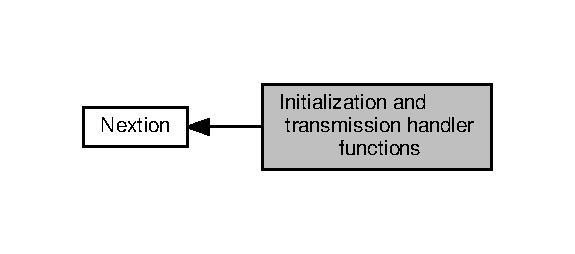
\includegraphics[width=276pt]{da/dcd/group__nextion___init}
\end{center}
\end{figure}
\subsection*{Functions}
\begin{DoxyCompactItemize}
\item 
void \hyperlink{group__nextion___init_ga954125e92a78b714cd63c21a481762a1}{nextion\+\_\+init} (void)
\begin{DoxyCompactList}\small\item\em Initialize the nextion and set baudrate to 9600. \end{DoxyCompactList}\item 
void \hyperlink{group__nextion___init_ga0ca6fd0e6f77921dd1123539857ba0a8}{U\+S\+A\+R\+T2\+\_\+\+I\+R\+Q\+Handler} (void)
\begin{DoxyCompactList}\small\item\em Global interrupt handler for U\+S\+A\+R\+T2. \end{DoxyCompactList}\item 
void \hyperlink{group__nextion___init_gac201b60d58b0eba2ce0b55710eb3c4d0}{D\+M\+A1\+\_\+\+Stream5\+\_\+\+I\+R\+Q\+Handler} (void)
\begin{DoxyCompactList}\small\item\em Global interrupt handler for D\+M\+A1 stream5. \end{DoxyCompactList}\item 
void \hyperlink{group__nextion___init_gae39a2c7ff1a319a65e808d8524ffcf18}{nextion\+\_\+buffer\+\_\+update} (void)
\end{DoxyCompactItemize}


\subsection{Detailed Description}
nextion initialization functions 



\subsection{Function Documentation}
\index{Initialization and transmission handler functions@{Initialization and transmission handler functions}!D\+M\+A1\+\_\+\+Stream5\+\_\+\+I\+R\+Q\+Handler@{D\+M\+A1\+\_\+\+Stream5\+\_\+\+I\+R\+Q\+Handler}}
\index{D\+M\+A1\+\_\+\+Stream5\+\_\+\+I\+R\+Q\+Handler@{D\+M\+A1\+\_\+\+Stream5\+\_\+\+I\+R\+Q\+Handler}!Initialization and transmission handler functions@{Initialization and transmission handler functions}}
\subsubsection[{\texorpdfstring{D\+M\+A1\+\_\+\+Stream5\+\_\+\+I\+R\+Q\+Handler(void)}{DMA1_Stream5_IRQHandler(void)}}]{\setlength{\rightskip}{0pt plus 5cm}void D\+M\+A1\+\_\+\+Stream5\+\_\+\+I\+R\+Q\+Handler (
\begin{DoxyParamCaption}
\item[{void}]{}
\end{DoxyParamCaption}
)}\hypertarget{group__nextion___init_gac201b60d58b0eba2ce0b55710eb3c4d0}{}\label{group__nextion___init_gac201b60d58b0eba2ce0b55710eb3c4d0}


Global interrupt handler for D\+M\+A1 stream5. 

\begin{DoxyNote}{Note}
Except memcpy, there is no functions used to 
\end{DoxyNote}
Transfer could be completed by 2 events\+:
\begin{DoxyItemize}
\item All data actually transfered (N\+D\+TR = 0)
\item Stream disabled inside U\+S\+A\+RT I\+D\+LE line detected interrupt (N\+D\+TR != 0)
\end{DoxyItemize}

Definition at line 156 of file N\+P\+S\+C\+\_\+nextion.\+c.

\index{Initialization and transmission handler functions@{Initialization and transmission handler functions}!nextion\+\_\+buffer\+\_\+update@{nextion\+\_\+buffer\+\_\+update}}
\index{nextion\+\_\+buffer\+\_\+update@{nextion\+\_\+buffer\+\_\+update}!Initialization and transmission handler functions@{Initialization and transmission handler functions}}
\subsubsection[{\texorpdfstring{nextion\+\_\+buffer\+\_\+update(void)}{nextion_buffer_update(void)}}]{\setlength{\rightskip}{0pt plus 5cm}void nextion\+\_\+buffer\+\_\+update (
\begin{DoxyParamCaption}
\item[{void}]{}
\end{DoxyParamCaption}
)}\hypertarget{group__nextion___init_gae39a2c7ff1a319a65e808d8524ffcf18}{}\label{group__nextion___init_gae39a2c7ff1a319a65e808d8524ffcf18}
M\+U\+ST BE A T\+A\+SK Loop data back to U\+A\+RT data register

Definition at line 120 of file N\+P\+S\+C\+\_\+nextion.\+c.

\index{Initialization and transmission handler functions@{Initialization and transmission handler functions}!nextion\+\_\+init@{nextion\+\_\+init}}
\index{nextion\+\_\+init@{nextion\+\_\+init}!Initialization and transmission handler functions@{Initialization and transmission handler functions}}
\subsubsection[{\texorpdfstring{nextion\+\_\+init(void)}{nextion_init(void)}}]{\setlength{\rightskip}{0pt plus 5cm}void nextion\+\_\+init (
\begin{DoxyParamCaption}
\item[{void}]{}
\end{DoxyParamCaption}
)}\hypertarget{group__nextion___init_ga954125e92a78b714cd63c21a481762a1}{}\label{group__nextion___init_ga954125e92a78b714cd63c21a481762a1}


Initialize the nextion and set baudrate to 9600. 


\begin{DoxyParams}{Parameters}
{\em None} & \\
\hline
\end{DoxyParams}

\begin{DoxyRetVals}{Return values}
{\em None} & \\
\hline
\end{DoxyRetVals}


Definition at line 47 of file N\+P\+S\+C\+\_\+nextion.\+c.



Here is the caller graph for this function\+:\nopagebreak
\begin{figure}[H]
\begin{center}
\leavevmode
\includegraphics[width=238pt]{da/dcd/group__nextion___init_ga954125e92a78b714cd63c21a481762a1_icgraph}
\end{center}
\end{figure}


\index{Initialization and transmission handler functions@{Initialization and transmission handler functions}!U\+S\+A\+R\+T2\+\_\+\+I\+R\+Q\+Handler@{U\+S\+A\+R\+T2\+\_\+\+I\+R\+Q\+Handler}}
\index{U\+S\+A\+R\+T2\+\_\+\+I\+R\+Q\+Handler@{U\+S\+A\+R\+T2\+\_\+\+I\+R\+Q\+Handler}!Initialization and transmission handler functions@{Initialization and transmission handler functions}}
\subsubsection[{\texorpdfstring{U\+S\+A\+R\+T2\+\_\+\+I\+R\+Q\+Handler(void)}{USART2_IRQHandler(void)}}]{\setlength{\rightskip}{0pt plus 5cm}void U\+S\+A\+R\+T2\+\_\+\+I\+R\+Q\+Handler (
\begin{DoxyParamCaption}
\item[{void}]{}
\end{DoxyParamCaption}
)}\hypertarget{group__nextion___init_ga0ca6fd0e6f77921dd1123539857ba0a8}{}\label{group__nextion___init_ga0ca6fd0e6f77921dd1123539857ba0a8}


Global interrupt handler for U\+S\+A\+R\+T2. 



Definition at line 138 of file N\+P\+S\+C\+\_\+nextion.\+c.


\hypertarget{group__nextion___trans}{}\section{Transmission functions}
\label{group__nextion___trans}\index{Transmission functions@{Transmission functions}}


nextion transmission functions  


Collaboration diagram for Transmission functions\+:\nopagebreak
\begin{figure}[H]
\begin{center}
\leavevmode
\includegraphics[width=284pt]{d5/d2e/group__nextion___trans}
\end{center}
\end{figure}
\subsection*{Functions}
\begin{DoxyCompactItemize}
\item 
void \hyperlink{group__nextion___trans_gae98be4e53e6ea89bf691feafaa79c18e}{nextion\+\_\+send} (uint8\+\_\+t $\ast$data)
\begin{DoxyCompactList}\small\item\em send string to the hc-\/06 \end{DoxyCompactList}\end{DoxyCompactItemize}


\subsection{Detailed Description}
nextion transmission functions 



\subsection{Function Documentation}
\index{Transmission functions@{Transmission functions}!nextion\+\_\+send@{nextion\+\_\+send}}
\index{nextion\+\_\+send@{nextion\+\_\+send}!Transmission functions@{Transmission functions}}
\subsubsection[{\texorpdfstring{nextion\+\_\+send(uint8\+\_\+t $\ast$data)}{nextion_send(uint8_t *data)}}]{\setlength{\rightskip}{0pt plus 5cm}void nextion\+\_\+send (
\begin{DoxyParamCaption}
\item[{uint8\+\_\+t $\ast$}]{data}
\end{DoxyParamCaption}
)}\hypertarget{group__nextion___trans_gae98be4e53e6ea89bf691feafaa79c18e}{}\label{group__nextion___trans_gae98be4e53e6ea89bf691feafaa79c18e}


send string to the hc-\/06 


\begin{DoxyParams}{Parameters}
{\em data} & string to be sent \\
\hline
\end{DoxyParams}

\begin{DoxyRetVals}{Return values}
{\em None} & \\
\hline
\end{DoxyRetVals}


Definition at line 217 of file N\+P\+S\+C\+\_\+nextion.\+c.


\hypertarget{group___audio}{}\section{Audio}
\label{group___audio}\index{Audio@{Audio}}


Manage audio configuration and play audio.  


Collaboration diagram for Audio\+:
% FIG 0
\subsection*{Modules}
\begin{DoxyCompactItemize}
\item 
\hyperlink{group___constant}{Constant}
\begin{DoxyCompactList}\small\item\em Define audio frequency and D\+MA frequency. \end{DoxyCompactList}\item 
\hyperlink{group___audio___init}{Configuration functions}
\begin{DoxyCompactList}\small\item\em Audio configuration functions. \end{DoxyCompactList}\item 
\hyperlink{group___audio___play}{Play audio functions}
\begin{DoxyCompactList}\small\item\em Audio functions. \end{DoxyCompactList}\end{DoxyCompactItemize}
\subsection*{Functions}
\begin{DoxyCompactItemize}
\item 
void \hyperlink{group___audio_gafff6cd7f4332d078ce0114143cd30998}{audio\+\_\+disable} (void)
\begin{DoxyCompactList}\small\item\em Disable the D\+MA. \end{DoxyCompactList}\item 
void \hyperlink{group___audio_ga6a621a84280fa05373990982dacce11b}{audio\+\_\+init} (uint16\+\_\+t $\ast$, uint16\+\_\+t)
\begin{DoxyCompactList}\small\item\em Perform audio initialization. \end{DoxyCompactList}\item 
void \hyperlink{group___audio_ga286b07d3729ae2bfdf88bcd777dd93cf}{audio\+\_\+play} (uint16\+\_\+t $\ast$, uint16\+\_\+t)
\begin{DoxyCompactList}\small\item\em Play a sample. \end{DoxyCompactList}\end{DoxyCompactItemize}


\subsection{Detailed Description}
Manage audio configuration and play audio. 



\subsection{Function Documentation}
\mbox{\Hypertarget{group___audio_gafff6cd7f4332d078ce0114143cd30998}\label{group___audio_gafff6cd7f4332d078ce0114143cd30998}} 
\index{Audio@{Audio}!audio\+\_\+disable@{audio\+\_\+disable}}
\index{audio\+\_\+disable@{audio\+\_\+disable}!Audio@{Audio}}
\subsubsection{\texorpdfstring{audio\+\_\+disable()}{audio\_disable()}}
{\footnotesize\ttfamily void audio\+\_\+disable (\begin{DoxyParamCaption}\item[{void}]{ }\end{DoxyParamCaption})}



Disable the D\+MA. 


\begin{DoxyParams}{Parameters}
{\em None} & \\
\hline
\end{DoxyParams}

\begin{DoxyRetVals}{Return values}
{\em None} & \\
\hline
\end{DoxyRetVals}
\mbox{\Hypertarget{group___audio_ga6a621a84280fa05373990982dacce11b}\label{group___audio_ga6a621a84280fa05373990982dacce11b}} 
\index{Audio@{Audio}!audio\+\_\+init@{audio\+\_\+init}}
\index{audio\+\_\+init@{audio\+\_\+init}!Audio@{Audio}}
\subsubsection{\texorpdfstring{audio\+\_\+init()}{audio\_init()}}
{\footnotesize\ttfamily void audio\+\_\+init (\begin{DoxyParamCaption}\item[{uint16\+\_\+t $\ast$}]{D\+A\+C\+Buffer,  }\item[{uint16\+\_\+t}]{Size }\end{DoxyParamCaption})}



Perform audio initialization. 


\begin{DoxyParams}{Parameters}
{\em D\+A\+C\+Buffer} & Array to be pushed to the D\+MA \\
\hline
{\em Mode} & D\+MA Mode (default\+:D\+M\+A\+\_\+\+Mode\+\_\+\+Normal) \\
\hline
{\em Size} & sample size (default\+:S\+A\+M\+P\+L\+E\+\_\+\+S\+I\+ZE) \\
\hline
\end{DoxyParams}

\begin{DoxyRetVals}{Return values}
{\em None} & \\
\hline
\end{DoxyRetVals}
\mbox{\Hypertarget{group___audio_ga286b07d3729ae2bfdf88bcd777dd93cf}\label{group___audio_ga286b07d3729ae2bfdf88bcd777dd93cf}} 
\index{Audio@{Audio}!audio\+\_\+play@{audio\+\_\+play}}
\index{audio\+\_\+play@{audio\+\_\+play}!Audio@{Audio}}
\subsubsection{\texorpdfstring{audio\+\_\+play()}{audio\_play()}}
{\footnotesize\ttfamily void audio\+\_\+play (\begin{DoxyParamCaption}\item[{uint16\+\_\+t $\ast$}]{D\+A\+C\+Buffer,  }\item[{uint16\+\_\+t}]{Size }\end{DoxyParamCaption})}



Play a sample. 


\begin{DoxyParams}{Parameters}
{\em D\+A\+C\+Buffer} & Array to be pushed to the D\+MA \\
\hline
{\em Size} & sample size (default\+:S\+A\+M\+P\+L\+E\+\_\+\+S\+I\+ZE) \\
\hline
\end{DoxyParams}
\begin{DoxyReturn}{Returns}
None 
\end{DoxyReturn}

\hypertarget{group__bluetooth}{}\section{Bluetooth}
\label{group__bluetooth}\index{Bluetooth@{Bluetooth}}


bluetooth driver modules  


Collaboration diagram for Bluetooth\+:\nopagebreak
\begin{figure}[H]
\begin{center}
\leavevmode
\includegraphics[width=350pt]{d3/ddb/group__bluetooth}
\end{center}
\end{figure}
\subsection*{Modules}
\begin{DoxyCompactItemize}
\item 
\hyperlink{group__bluetooth___constants}{Bluetooth\+\_\+\+Constants}
\begin{DoxyCompactList}\small\item\em define bluetooth constant \end{DoxyCompactList}\item 
\hyperlink{group__bluetooth___init}{Initialization and transmission handler functions}
\begin{DoxyCompactList}\small\item\em bluetooth initialization functions \end{DoxyCompactList}\item 
\hyperlink{group__bluetooth___trans}{Transmission functions}
\begin{DoxyCompactList}\small\item\em bluetooth transmission functions \end{DoxyCompactList}\end{DoxyCompactItemize}
\subsection*{Variables}
\begin{DoxyCompactItemize}
\item 
size\+\_\+t \hyperlink{group__bluetooth_ga7143c37ba48173d0e245161e9ddc3592}{bluetooth\+\_\+write}
\item 
size\+\_\+t \hyperlink{group__bluetooth_ga723054cd6b30ca246f123b25e099146d}{bluetooth\+\_\+read}
\end{DoxyCompactItemize}


\subsection{Detailed Description}
bluetooth driver modules 



\subsection{Variable Documentation}
\index{Bluetooth@{Bluetooth}!bluetooth\+\_\+read@{bluetooth\+\_\+read}}
\index{bluetooth\+\_\+read@{bluetooth\+\_\+read}!Bluetooth@{Bluetooth}}
\subsubsection[{\texorpdfstring{bluetooth\+\_\+read}{bluetooth_read}}]{\setlength{\rightskip}{0pt plus 5cm}size\+\_\+t bluetooth\+\_\+read}\hypertarget{group__bluetooth_ga723054cd6b30ca246f123b25e099146d}{}\label{group__bluetooth_ga723054cd6b30ca246f123b25e099146d}


Definition at line 56 of file N\+P\+C\+\_\+bluetooth.\+h.

\index{Bluetooth@{Bluetooth}!bluetooth\+\_\+write@{bluetooth\+\_\+write}}
\index{bluetooth\+\_\+write@{bluetooth\+\_\+write}!Bluetooth@{Bluetooth}}
\subsubsection[{\texorpdfstring{bluetooth\+\_\+write}{bluetooth_write}}]{\setlength{\rightskip}{0pt plus 5cm}size\+\_\+t bluetooth\+\_\+write}\hypertarget{group__bluetooth_ga7143c37ba48173d0e245161e9ddc3592}{}\label{group__bluetooth_ga7143c37ba48173d0e245161e9ddc3592}


Definition at line 56 of file N\+P\+C\+\_\+bluetooth.\+h.


\hypertarget{group___clock}{}\section{Clock}
\label{group___clock}\index{Clock@{Clock}}


Clock driver modules.  


Collaboration diagram for Clock\+:
% FIG 0
\subsection*{Modules}
\begin{DoxyCompactItemize}
\item 
\hyperlink{group___r_t_c___p_r_e_d_i_v___definitions}{R\+T\+C\+\_\+\+P\+R\+E\+D\+I\+V\+\_\+\+Definitions}
\begin{DoxyCompactList}\small\item\em definition of prescaler for Asynchronous and Synchronous \end{DoxyCompactList}\item 
\hyperlink{group___c_l_o_c_k___choice}{C\+L\+O\+C\+K\+\_\+\+Choice}
\begin{DoxyCompactList}\small\item\em Clock A or B. \end{DoxyCompactList}\item 
\hyperlink{group___c_l_o_c_k___format}{C\+L\+O\+C\+K\+\_\+\+Format}
\begin{DoxyCompactList}\small\item\em AM or PM. \end{DoxyCompactList}\item 
\hyperlink{group___c_l_o_c_k___value}{C\+L\+O\+C\+K\+\_\+\+Value}
\begin{DoxyCompactList}\small\item\em Access time or date parameters. \end{DoxyCompactList}\item 
\hyperlink{group___r_e_p_e_a_t___definitions}{R\+E\+P\+E\+A\+T\+\_\+\+Definitions}
\begin{DoxyCompactList}\small\item\em Alarm repeat options. \end{DoxyCompactList}\item 
\hyperlink{group___clock___init}{Initialisation functions}
\begin{DoxyCompactList}\small\item\em Clock initialisation functions. \end{DoxyCompactList}\item 
\hyperlink{group___clock___time___date}{Time and Date Configuration functions}
\begin{DoxyCompactList}\small\item\em Clock time and date configuration functions. \end{DoxyCompactList}\item 
\hyperlink{group___clock___alarms}{Alarms configuration functions}
\begin{DoxyCompactList}\small\item\em Clock alarm configuration functions. \end{DoxyCompactList}\end{DoxyCompactItemize}
\subsection*{Functions}
\begin{DoxyCompactItemize}
\item 
void \hyperlink{group___clock_ga78ab77b57cf2e00089f0a3a22508524c}{clock\+\_\+init} (void)
\begin{DoxyCompactList}\small\item\em Initialise the clock to 1\+Hz and setup peripherals for Alarm. \end{DoxyCompactList}\item 
Error\+Status \hyperlink{group___clock_gaf16498fa2702bfda6b89a3335ccc7ca6}{clock\+\_\+set\+Date} (uint8\+\_\+t week\+Day, uint8\+\_\+t month, uint8\+\_\+t date, uint8\+\_\+t year)
\begin{DoxyCompactList}\small\item\em Set the clock\textquotesingle{}s date. \end{DoxyCompactList}\item 
Error\+Status \hyperlink{group___clock_ga11404197d58ddf6b46230bcde4282ef2}{clock\+\_\+set\+Time} (uint8\+\_\+t am\+\_\+pm, uint8\+\_\+t hours, uint8\+\_\+t minutes, uint8\+\_\+t second)
\begin{DoxyCompactList}\small\item\em Set the clock\textquotesingle{}s time. \end{DoxyCompactList}\item 
uint32\+\_\+t \hyperlink{group___clock_gabb4d72928cb3d131d40067fb141003aa}{clock\+\_\+get\+Date} (void)
\begin{DoxyCompactList}\small\item\em Get the date encoded in a 32b format. \end{DoxyCompactList}\item 
uint32\+\_\+t \hyperlink{group___clock_ga03ae6948083c259f6edc0b146f40dc62}{clock\+\_\+get\+Time} (void)
\begin{DoxyCompactList}\small\item\em Get the time encoded in a 32b format. \end{DoxyCompactList}\item 
R\+T\+C\+\_\+\+Alarm\+Type\+Def \hyperlink{group___clock_ga5e1614dbb1a210106dbade3f133db27e}{clock\+\_\+create\+Alarm} (uint8\+\_\+t am\+\_\+pm, uint8\+\_\+t hours, uint8\+\_\+t minutes, uint8\+\_\+t seconds, uint32\+\_\+t date\+Week\+Day\+Sel, uint8\+\_\+t date\+Week\+Day, uint32\+\_\+t repeat)
\begin{DoxyCompactList}\small\item\em Create an Alarm Structure given all the parameters. \end{DoxyCompactList}\item 
void \hyperlink{group___clock_gab56f512746d4f2638232db28bb7dac2b}{clock\+\_\+setA} (R\+T\+C\+\_\+\+Alarm\+Type\+Def $\ast$Alarm)
\begin{DoxyCompactList}\small\item\em Set an alarm to R\+T\+C\+\_\+\+Alarm\+\_\+A, given a Alarm structure R\+T\+C\+\_\+\+Alarm\+Type\+Def. \end{DoxyCompactList}\item 
void \hyperlink{group___clock_gaea1a099c4ad6de8b99517ac6453e3569}{clock\+\_\+set\+Alarm} (uint8\+\_\+t am\+\_\+pm, uint8\+\_\+t hours, uint8\+\_\+t minutes, uint8\+\_\+t seconds, uint32\+\_\+t date\+Week\+Day\+Sel, uint8\+\_\+t date\+Week\+Day, uint32\+\_\+t repeat)
\begin{DoxyCompactList}\small\item\em Set an alarm to R\+T\+C\+\_\+\+Alarm\+\_\+A, given all the alarm parameters. \end{DoxyCompactList}\item 
void \hyperlink{group___clock_ga4da4fb52ec579671d337938e78f9a207}{R\+T\+C\+\_\+\+Alarm\+\_\+\+I\+R\+Q\+Handler} (void)
\begin{DoxyCompactList}\small\item\em Alarm Handler. \end{DoxyCompactList}\end{DoxyCompactItemize}
\subsection*{Variables}
\begin{DoxyCompactItemize}
\item 
\mbox{\Hypertarget{group___clock_gab350523f036d8469fd207d7144f7e385}\label{group___clock_gab350523f036d8469fd207d7144f7e385}} 
R\+T\+C\+\_\+\+Time\+Type\+Def {\bfseries R\+T\+C\+\_\+\+Time\+Struct}
\item 
\mbox{\Hypertarget{group___clock_gabd73cfb4bb5c20ec4524dd5fe244842b}\label{group___clock_gabd73cfb4bb5c20ec4524dd5fe244842b}} 
R\+T\+C\+\_\+\+Init\+Type\+Def {\bfseries R\+T\+C\+\_\+\+Init\+Struct}
\item 
\mbox{\Hypertarget{group___clock_gaa57dd593e8f26c6f126fd0f694a1facc}\label{group___clock_gaa57dd593e8f26c6f126fd0f694a1facc}} 
R\+T\+C\+\_\+\+Date\+Type\+Def {\bfseries R\+T\+C\+\_\+\+Date\+Strcut}
\item 
\mbox{\Hypertarget{group___clock_ga64d4fe2aa4668079f349f9eb97a48e35}\label{group___clock_ga64d4fe2aa4668079f349f9eb97a48e35}} 
R\+T\+C\+\_\+\+Alarm\+Type\+Def {\bfseries R\+T\+C\+\_\+\+Alarm\+Struct}
\item 
\mbox{\Hypertarget{group___clock_gaf0f09eb6c46f0a7cc5f7736c709a8c77}\label{group___clock_gaf0f09eb6c46f0a7cc5f7736c709a8c77}} 
E\+X\+T\+I\+\_\+\+Init\+Type\+Def {\bfseries E\+X\+T\+I\+\_\+\+Init\+Struct}
\end{DoxyCompactItemize}


\subsection{Detailed Description}
Clock driver modules. 



\subsection{Function Documentation}
\mbox{\Hypertarget{group___clock_ga5e1614dbb1a210106dbade3f133db27e}\label{group___clock_ga5e1614dbb1a210106dbade3f133db27e}} 
\index{Clock@{Clock}!clock\+\_\+create\+Alarm@{clock\+\_\+create\+Alarm}}
\index{clock\+\_\+create\+Alarm@{clock\+\_\+create\+Alarm}!Clock@{Clock}}
\subsubsection{\texorpdfstring{clock\+\_\+create\+Alarm()}{clock\_createAlarm()}}
{\footnotesize\ttfamily R\+T\+C\+\_\+\+Alarm\+Type\+Def clock\+\_\+create\+Alarm (\begin{DoxyParamCaption}\item[{uint8\+\_\+t}]{am\+\_\+pm,  }\item[{uint8\+\_\+t}]{hours,  }\item[{uint8\+\_\+t}]{minutes,  }\item[{uint8\+\_\+t}]{seconds,  }\item[{uint32\+\_\+t}]{date\+Week\+Day\+Sel,  }\item[{uint8\+\_\+t}]{date\+Week\+Day,  }\item[{uint32\+\_\+t}]{repeat }\end{DoxyParamCaption})}



Create an Alarm Structure given all the parameters. 


\begin{DoxyParams}{Parameters}
{\em am\+\_\+pm} & AM PM format (C\+L\+O\+C\+K\+\_\+\+AM) \\
\hline
{\em hours} & Alarm hours \\
\hline
{\em minutes} & Alarm minutes \\
\hline
{\em seconds} & Alarm seconds \\
\hline
{\em date\+Week\+Day\+Sel} & Date of Week\+Day selection R\+T\+C\+\_\+\+Alarm\+Date\+Week\+Day\+\_\+\+Definitions \\
\hline
{\em date\+Week\+Day} & Specify Alarm Date/\+Weekday if Date then value range from 1-\/31, else R\+T\+C\+\_\+\+Week\+Day\+\_\+\+Definitions \\
\hline
{\em repeat} & Specify the repetition of the Alarm \\
\hline
\end{DoxyParams}

\begin{DoxyRetVals}{Return values}
{\em An} & R\+T\+C\+\_\+\+Alarm\+Type\+Def containing all the parameters above \\
\hline
\end{DoxyRetVals}
\mbox{\Hypertarget{group___clock_gabb4d72928cb3d131d40067fb141003aa}\label{group___clock_gabb4d72928cb3d131d40067fb141003aa}} 
\index{Clock@{Clock}!clock\+\_\+get\+Date@{clock\+\_\+get\+Date}}
\index{clock\+\_\+get\+Date@{clock\+\_\+get\+Date}!Clock@{Clock}}
\subsubsection{\texorpdfstring{clock\+\_\+get\+Date()}{clock\_getDate()}}
{\footnotesize\ttfamily uint32\+\_\+t clock\+\_\+get\+Date (\begin{DoxyParamCaption}\item[{void}]{ }\end{DoxyParamCaption})}



Get the date encoded in a 32b format. 


\begin{DoxyParams}{Parameters}
{\em None} & \\
\hline
\end{DoxyParams}

\begin{DoxyRetVals}{Return values}
{\em An} & uint32\+\_\+t containing the week\+Day as its M\+B3, date \+: M\+B2, month \+: M\+B1, year \+: M\+B0 \\
\hline
\end{DoxyRetVals}
\mbox{\Hypertarget{group___clock_ga03ae6948083c259f6edc0b146f40dc62}\label{group___clock_ga03ae6948083c259f6edc0b146f40dc62}} 
\index{Clock@{Clock}!clock\+\_\+get\+Time@{clock\+\_\+get\+Time}}
\index{clock\+\_\+get\+Time@{clock\+\_\+get\+Time}!Clock@{Clock}}
\subsubsection{\texorpdfstring{clock\+\_\+get\+Time()}{clock\_getTime()}}
{\footnotesize\ttfamily uint32\+\_\+t clock\+\_\+get\+Time (\begin{DoxyParamCaption}\item[{void}]{ }\end{DoxyParamCaption})}



Get the time encoded in a 32b format. 


\begin{DoxyParams}{Parameters}
{\em None} & \\
\hline
\end{DoxyParams}

\begin{DoxyRetVals}{Return values}
{\em An} & uint32\+\_\+t containing the hour as its M\+B3, minutes \+: M\+B2, Seconds \+: M\+B1, format \+: M\+B0 \\
\hline
\end{DoxyRetVals}
\mbox{\Hypertarget{group___clock_ga78ab77b57cf2e00089f0a3a22508524c}\label{group___clock_ga78ab77b57cf2e00089f0a3a22508524c}} 
\index{Clock@{Clock}!clock\+\_\+init@{clock\+\_\+init}}
\index{clock\+\_\+init@{clock\+\_\+init}!Clock@{Clock}}
\subsubsection{\texorpdfstring{clock\+\_\+init()}{clock\_init()}}
{\footnotesize\ttfamily void clock\+\_\+init (\begin{DoxyParamCaption}\item[{void}]{ }\end{DoxyParamCaption})}



Initialise the clock to 1\+Hz and setup peripherals for Alarm. 


\begin{DoxyParams}{Parameters}
{\em None} & \\
\hline
\end{DoxyParams}

\begin{DoxyRetVals}{Return values}
{\em None} & \\
\hline
\end{DoxyRetVals}
\mbox{\Hypertarget{group___clock_gab56f512746d4f2638232db28bb7dac2b}\label{group___clock_gab56f512746d4f2638232db28bb7dac2b}} 
\index{Clock@{Clock}!clock\+\_\+setA@{clock\+\_\+setA}}
\index{clock\+\_\+setA@{clock\+\_\+setA}!Clock@{Clock}}
\subsubsection{\texorpdfstring{clock\+\_\+set\+A()}{clock\_setA()}}
{\footnotesize\ttfamily void clock\+\_\+setA (\begin{DoxyParamCaption}\item[{R\+T\+C\+\_\+\+Alarm\+Type\+Def $\ast$}]{Alarm }\end{DoxyParamCaption})}



Set an alarm to R\+T\+C\+\_\+\+Alarm\+\_\+A, given a Alarm structure R\+T\+C\+\_\+\+Alarm\+Type\+Def. 


\begin{DoxyParams}{Parameters}
{\em Alarm} & A pointer to the R\+T\+C\+\_\+\+Alarm\+Type\+Def \\
\hline
\end{DoxyParams}

\begin{DoxyRetVals}{Return values}
{\em None} & \\
\hline
\end{DoxyRetVals}
\mbox{\Hypertarget{group___clock_gaea1a099c4ad6de8b99517ac6453e3569}\label{group___clock_gaea1a099c4ad6de8b99517ac6453e3569}} 
\index{Clock@{Clock}!clock\+\_\+set\+Alarm@{clock\+\_\+set\+Alarm}}
\index{clock\+\_\+set\+Alarm@{clock\+\_\+set\+Alarm}!Clock@{Clock}}
\subsubsection{\texorpdfstring{clock\+\_\+set\+Alarm()}{clock\_setAlarm()}}
{\footnotesize\ttfamily void clock\+\_\+set\+Alarm (\begin{DoxyParamCaption}\item[{uint8\+\_\+t}]{am\+\_\+pm,  }\item[{uint8\+\_\+t}]{hours,  }\item[{uint8\+\_\+t}]{minutes,  }\item[{uint8\+\_\+t}]{seconds,  }\item[{uint32\+\_\+t}]{date\+Week\+Day\+Sel,  }\item[{uint8\+\_\+t}]{date\+Week\+Day,  }\item[{uint32\+\_\+t}]{repeat }\end{DoxyParamCaption})}



Set an alarm to R\+T\+C\+\_\+\+Alarm\+\_\+A, given all the alarm parameters. 


\begin{DoxyParams}{Parameters}
{\em am\+\_\+pm} & AM PM format (C\+L\+O\+C\+K\+\_\+\+AM) \\
\hline
{\em hours} & Alarm hours \\
\hline
{\em minutes} & Alarm minutes \\
\hline
{\em seconds} & Alarm seconds \\
\hline
{\em date\+Week\+Day\+Sel} & Date of Week\+Day selection R\+T\+C\+\_\+\+Alarm\+Date\+Week\+Day\+\_\+\+Definitions \\
\hline
{\em date\+Week\+Day} & Specify Alarm Date/\+Weekday if Date then value range from 1-\/31, else R\+T\+C\+\_\+\+Week\+Day\+\_\+\+Definitions \\
\hline
{\em repeat} & Specify the repetition of the Alarm \\
\hline
\end{DoxyParams}

\begin{DoxyRetVals}{Return values}
{\em None} & \\
\hline
\end{DoxyRetVals}
\mbox{\Hypertarget{group___clock_gaf16498fa2702bfda6b89a3335ccc7ca6}\label{group___clock_gaf16498fa2702bfda6b89a3335ccc7ca6}} 
\index{Clock@{Clock}!clock\+\_\+set\+Date@{clock\+\_\+set\+Date}}
\index{clock\+\_\+set\+Date@{clock\+\_\+set\+Date}!Clock@{Clock}}
\subsubsection{\texorpdfstring{clock\+\_\+set\+Date()}{clock\_setDate()}}
{\footnotesize\ttfamily Error\+Status clock\+\_\+set\+Date (\begin{DoxyParamCaption}\item[{uint8\+\_\+t}]{week\+Day,  }\item[{uint8\+\_\+t}]{month,  }\item[{uint8\+\_\+t}]{date,  }\item[{uint8\+\_\+t}]{year }\end{DoxyParamCaption})}



Set the clock\textquotesingle{}s date. 


\begin{DoxyParams}{Parameters}
{\em None} & \\
\hline
\end{DoxyParams}

\begin{DoxyRetVals}{Return values}
{\em Error\+Status} & representing the outcome of the operation
\begin{DoxyItemize}
\item S\+U\+C\+C\+E\+SS\+: R\+TC Shift registers are configured
\item E\+R\+R\+OR\+: R\+TC Shift registers are not configured 
\end{DoxyItemize}\\
\hline
\end{DoxyRetVals}
\mbox{\Hypertarget{group___clock_ga11404197d58ddf6b46230bcde4282ef2}\label{group___clock_ga11404197d58ddf6b46230bcde4282ef2}} 
\index{Clock@{Clock}!clock\+\_\+set\+Time@{clock\+\_\+set\+Time}}
\index{clock\+\_\+set\+Time@{clock\+\_\+set\+Time}!Clock@{Clock}}
\subsubsection{\texorpdfstring{clock\+\_\+set\+Time()}{clock\_setTime()}}
{\footnotesize\ttfamily Error\+Status clock\+\_\+set\+Time (\begin{DoxyParamCaption}\item[{uint8\+\_\+t}]{am\+\_\+pm,  }\item[{uint8\+\_\+t}]{hours,  }\item[{uint8\+\_\+t}]{minutes,  }\item[{uint8\+\_\+t}]{second }\end{DoxyParamCaption})}



Set the clock\textquotesingle{}s time. 


\begin{DoxyParams}{Parameters}
{\em None} & \\
\hline
\end{DoxyParams}

\begin{DoxyRetVals}{Return values}
{\em Error\+Status} & representing the outcome of the operation
\begin{DoxyItemize}
\item S\+U\+C\+C\+E\+SS\+: R\+TC Shift registers are configured
\item E\+R\+R\+OR\+: R\+TC Shift registers are not configured 
\end{DoxyItemize}\\
\hline
\end{DoxyRetVals}
\mbox{\Hypertarget{group___clock_ga4da4fb52ec579671d337938e78f9a207}\label{group___clock_ga4da4fb52ec579671d337938e78f9a207}} 
\index{Clock@{Clock}!R\+T\+C\+\_\+\+Alarm\+\_\+\+I\+R\+Q\+Handler@{R\+T\+C\+\_\+\+Alarm\+\_\+\+I\+R\+Q\+Handler}}
\index{R\+T\+C\+\_\+\+Alarm\+\_\+\+I\+R\+Q\+Handler@{R\+T\+C\+\_\+\+Alarm\+\_\+\+I\+R\+Q\+Handler}!Clock@{Clock}}
\subsubsection{\texorpdfstring{R\+T\+C\+\_\+\+Alarm\+\_\+\+I\+R\+Q\+Handler()}{RTC\_Alarm\_IRQHandler()}}
{\footnotesize\ttfamily void R\+T\+C\+\_\+\+Alarm\+\_\+\+I\+R\+Q\+Handler (\begin{DoxyParamCaption}\item[{void}]{ }\end{DoxyParamCaption})}



Alarm Handler. 


\begin{DoxyParams}{Parameters}
{\em None} & \\
\hline
\end{DoxyParams}

\begin{DoxyRetVals}{Return values}
{\em None} & \\
\hline
\end{DoxyRetVals}

\hypertarget{group___configuration}{}\section{Configuration}
\label{group___configuration}\index{Configuration@{Configuration}}


Configuration driver modules.  


\subsection*{Functions}
\begin{DoxyCompactItemize}
\item 
void \hyperlink{group___configuration_gabe73c51b6f7ce590321d186bef079fe4}{N\+P\+C\+\_\+init} (void)
\begin{DoxyCompactList}\small\item\em Initialize all firmwares used by the N\+PC. \end{DoxyCompactList}\item 
void \hyperlink{group___configuration_ga1730ffe1e560465665eb47d9264826f9}{Error\+\_\+\+Handler} (void)
\begin{DoxyCompactList}\small\item\em This function is executed in case of error occurrence. \end{DoxyCompactList}\end{DoxyCompactItemize}


\subsection{Detailed Description}
Configuration driver modules. 



\subsection{Function Documentation}
\mbox{\Hypertarget{group___configuration_ga1730ffe1e560465665eb47d9264826f9}\label{group___configuration_ga1730ffe1e560465665eb47d9264826f9}} 
\index{Configuration@{Configuration}!Error\+\_\+\+Handler@{Error\+\_\+\+Handler}}
\index{Error\+\_\+\+Handler@{Error\+\_\+\+Handler}!Configuration@{Configuration}}
\subsubsection{\texorpdfstring{Error\+\_\+\+Handler()}{Error\_Handler()}}
{\footnotesize\ttfamily void Error\+\_\+\+Handler (\begin{DoxyParamCaption}\item[{void}]{ }\end{DoxyParamCaption})}



This function is executed in case of error occurrence. 


\begin{DoxyParams}{Parameters}
{\em None} & \\
\hline
\end{DoxyParams}

\begin{DoxyRetVals}{Return values}
{\em None} & \\
\hline
\end{DoxyRetVals}
\mbox{\Hypertarget{group___configuration_gabe73c51b6f7ce590321d186bef079fe4}\label{group___configuration_gabe73c51b6f7ce590321d186bef079fe4}} 
\index{Configuration@{Configuration}!N\+P\+C\+\_\+init@{N\+P\+C\+\_\+init}}
\index{N\+P\+C\+\_\+init@{N\+P\+C\+\_\+init}!Configuration@{Configuration}}
\subsubsection{\texorpdfstring{N\+P\+C\+\_\+init()}{NPC\_init()}}
{\footnotesize\ttfamily void N\+P\+C\+\_\+init (\begin{DoxyParamCaption}\item[{void}]{ }\end{DoxyParamCaption})}



Initialize all firmwares used by the N\+PC. 


\begin{DoxyParams}{Parameters}
{\em None} & \\
\hline
\end{DoxyParams}

\begin{DoxyRetVals}{Return values}
{\em None} & \\
\hline
\end{DoxyRetVals}

\hypertarget{group___eeprom}{}\section{Eeprom}
\label{group___eeprom}\index{Eeprom@{Eeprom}}


Eeprom framework.  


\subsection*{Modules}
\begin{DoxyCompactItemize}
\item 
\hyperlink{group___instructions}{Instructions}
\begin{DoxyCompactList}\small\item\em 25\+L\+C640A instruction set \end{DoxyCompactList}\item 
\hyperlink{group___utilities}{Utilities}
\item 
\hyperlink{group___eeprom___init}{Initialisation functions}
\begin{DoxyCompactList}\small\item\em Eeprom initialisation functions. \end{DoxyCompactList}\item 
\hyperlink{group___eeprom___trans}{Transmission functions}
\begin{DoxyCompactList}\small\item\em Eeprom data transmission functions. \end{DoxyCompactList}\end{DoxyCompactItemize}
\subsection*{Functions}
\begin{DoxyCompactItemize}
\item 
void \hyperlink{group___eeprom_ga4ec7f9d780da432051aa74ec5892a94c}{eeprom\+\_\+init} (void)
\begin{DoxyCompactList}\small\item\em Initialise communication to the eeprom. \end{DoxyCompactList}\item 
void \hyperlink{group___eeprom_ga11e27abf76759a5907ef18d1351aecdb}{eeprom\+\_\+write} (uint16\+\_\+t address, uint8\+\_\+t data)
\begin{DoxyCompactList}\small\item\em Write a byte to the eeprom. \end{DoxyCompactList}\item 
uint8\+\_\+t \hyperlink{group___eeprom_gafaa7cca6f6ad1d9ae49522324c825c2f}{eeprom\+\_\+read} (uint16\+\_\+t address)
\begin{DoxyCompactList}\small\item\em Read a byte from the eeprom. \end{DoxyCompactList}\item 
void \hyperlink{group___eeprom_ga4f1a1c3f7642565b9dbff6bfd2e7ed0d}{eeprom\+\_\+write32\+Bytes} (uint16\+\_\+t base\+Address, uint8\+\_\+t $\ast$data)
\begin{DoxyCompactList}\small\item\em Write a page to the eeprom. \end{DoxyCompactList}\item 
void \hyperlink{group___eeprom_ga7964a5a66da1c4a59a42309a93752217}{eeprom\+\_\+clear} (void)
\begin{DoxyCompactList}\small\item\em Clear eeprom data. \end{DoxyCompactList}\end{DoxyCompactItemize}


\subsection{Detailed Description}
Eeprom framework. 



\subsection{Function Documentation}
\mbox{\Hypertarget{group___eeprom_ga7964a5a66da1c4a59a42309a93752217}\label{group___eeprom_ga7964a5a66da1c4a59a42309a93752217}} 
\index{Eeprom@{Eeprom}!eeprom\+\_\+clear@{eeprom\+\_\+clear}}
\index{eeprom\+\_\+clear@{eeprom\+\_\+clear}!Eeprom@{Eeprom}}
\subsubsection{\texorpdfstring{eeprom\+\_\+clear()}{eeprom\_clear()}}
{\footnotesize\ttfamily void eeprom\+\_\+clear (\begin{DoxyParamCaption}\item[{void}]{ }\end{DoxyParamCaption})}



Clear eeprom data. 


\begin{DoxyParams}{Parameters}
{\em None} & \\
\hline
\end{DoxyParams}

\begin{DoxyRetVals}{Return values}
{\em None} & \\
\hline
\end{DoxyRetVals}
\mbox{\Hypertarget{group___eeprom_ga4ec7f9d780da432051aa74ec5892a94c}\label{group___eeprom_ga4ec7f9d780da432051aa74ec5892a94c}} 
\index{Eeprom@{Eeprom}!eeprom\+\_\+init@{eeprom\+\_\+init}}
\index{eeprom\+\_\+init@{eeprom\+\_\+init}!Eeprom@{Eeprom}}
\subsubsection{\texorpdfstring{eeprom\+\_\+init()}{eeprom\_init()}}
{\footnotesize\ttfamily void eeprom\+\_\+init (\begin{DoxyParamCaption}\item[{void}]{ }\end{DoxyParamCaption})}



Initialise communication to the eeprom. 


\begin{DoxyParams}{Parameters}
{\em None} & \\
\hline
\end{DoxyParams}

\begin{DoxyRetVals}{Return values}
{\em None} & \\
\hline
\end{DoxyRetVals}
\mbox{\Hypertarget{group___eeprom_gafaa7cca6f6ad1d9ae49522324c825c2f}\label{group___eeprom_gafaa7cca6f6ad1d9ae49522324c825c2f}} 
\index{Eeprom@{Eeprom}!eeprom\+\_\+read@{eeprom\+\_\+read}}
\index{eeprom\+\_\+read@{eeprom\+\_\+read}!Eeprom@{Eeprom}}
\subsubsection{\texorpdfstring{eeprom\+\_\+read()}{eeprom\_read()}}
{\footnotesize\ttfamily uint8\+\_\+t eeprom\+\_\+read (\begin{DoxyParamCaption}\item[{uint16\+\_\+t}]{address }\end{DoxyParamCaption})}



Read a byte from the eeprom. 


\begin{DoxyParams}{Parameters}
{\em address} & The address of the memory \\
\hline
\end{DoxyParams}

\begin{DoxyRetVals}{Return values}
{\em uint8\+\_\+t} & data from eeprom \\
\hline
\end{DoxyRetVals}
\mbox{\Hypertarget{group___eeprom_ga11e27abf76759a5907ef18d1351aecdb}\label{group___eeprom_ga11e27abf76759a5907ef18d1351aecdb}} 
\index{Eeprom@{Eeprom}!eeprom\+\_\+write@{eeprom\+\_\+write}}
\index{eeprom\+\_\+write@{eeprom\+\_\+write}!Eeprom@{Eeprom}}
\subsubsection{\texorpdfstring{eeprom\+\_\+write()}{eeprom\_write()}}
{\footnotesize\ttfamily void eeprom\+\_\+write (\begin{DoxyParamCaption}\item[{uint16\+\_\+t}]{address,  }\item[{uint8\+\_\+t}]{data }\end{DoxyParamCaption})}



Write a byte to the eeprom. 


\begin{DoxyParams}{Parameters}
{\em address} & The address of th memory \\
\hline
{\em data} & The data to be written to the memory \\
\hline
\end{DoxyParams}

\begin{DoxyRetVals}{Return values}
{\em None} & \\
\hline
\end{DoxyRetVals}
\mbox{\Hypertarget{group___eeprom_ga4f1a1c3f7642565b9dbff6bfd2e7ed0d}\label{group___eeprom_ga4f1a1c3f7642565b9dbff6bfd2e7ed0d}} 
\index{Eeprom@{Eeprom}!eeprom\+\_\+write32\+Bytes@{eeprom\+\_\+write32\+Bytes}}
\index{eeprom\+\_\+write32\+Bytes@{eeprom\+\_\+write32\+Bytes}!Eeprom@{Eeprom}}
\subsubsection{\texorpdfstring{eeprom\+\_\+write32\+Bytes()}{eeprom\_write32Bytes()}}
{\footnotesize\ttfamily void eeprom\+\_\+write32\+Bytes (\begin{DoxyParamCaption}\item[{uint16\+\_\+t}]{base\+Address,  }\item[{uint8\+\_\+t $\ast$}]{data }\end{DoxyParamCaption})}



Write a page to the eeprom. 


\begin{DoxyParams}{Parameters}
{\em base\+Address} & The base address of the page \\
\hline
{\em data} & An array of data to be send \\
\hline
\end{DoxyParams}

\begin{DoxyRetVals}{Return values}
{\em None} & \\
\hline
\end{DoxyRetVals}

\hypertarget{group___neo_pixel}{}\section{Neo\+Pixel}
\label{group___neo_pixel}\index{Neo\+Pixel@{Neo\+Pixel}}


neopixel driver modules  


\subsection*{Modules}
\begin{DoxyCompactItemize}
\item 
\hyperlink{group___constant}{Constant}
\begin{DoxyCompactList}\small\item\em Define audio frequency and D\+MA frequency. \end{DoxyCompactList}\item 
\hyperlink{group___neo_pixel___init}{Initialisation functions}
\begin{DoxyCompactList}\small\item\em Neopixel initialisation functions. \end{DoxyCompactList}\item 
\hyperlink{group___neo_pixel___state}{State alteration functions}
\begin{DoxyCompactList}\small\item\em Neopixel state alteration functions. \end{DoxyCompactList}\item 
\hyperlink{group___neo_pixel___colour}{Colour generation functions}
\begin{DoxyCompactList}\small\item\em Neopixel colour functions. \end{DoxyCompactList}\item 
\hyperlink{group___neo_pixel___display}{colour display functions}
\begin{DoxyCompactList}\small\item\em Neopixel colour display functions. \end{DoxyCompactList}\end{DoxyCompactItemize}
\subsection*{Functions}
\begin{DoxyCompactItemize}
\item 
void \hyperlink{group___neo_pixel_gaac78468985e44a3e4d353ea9276b33bc}{neopixel\+\_\+init} (void)
\begin{DoxyCompactList}\small\item\em Initialise the neopixel. \end{DoxyCompactList}\item 
void \hyperlink{group___neo_pixel_gae027558106eef5c81996294f4561fecb}{neopixel\+\_\+set\+Brightness} (uint8\+\_\+t b)
\begin{DoxyCompactList}\small\item\em Set the brightness of the led. \end{DoxyCompactList}\item 
\mbox{\Hypertarget{group___neo_pixel_gada44b0356745943702c92d394760cd3e}\label{group___neo_pixel_gada44b0356745943702c92d394760cd3e}} 
void {\bfseries neopixel\+\_\+set\+State} (uint8\+\_\+t s)
\item 
\mbox{\Hypertarget{group___neo_pixel_gadb692027c25b23852a28f2ca43dc2399}\label{group___neo_pixel_gadb692027c25b23852a28f2ca43dc2399}} 
void {\bfseries neopixel\+\_\+show} (void)
\item 
void \hyperlink{group___neo_pixel_ga8e3cfef785ce221672f825f8785c25b8}{neopixel\+\_\+clear} (void)
\begin{DoxyCompactList}\small\item\em Stop pushing data to the neopixels. \end{DoxyCompactList}\item 
void \hyperlink{group___neo_pixel_ga79e34feddcfb2c45ae218166c84bdff4}{neopixel\+\_\+data\+Init} (void)
\begin{DoxyCompactList}\small\item\em Initialise the L\+E\+Dbuffer. \end{DoxyCompactList}\item 
void \hyperlink{group___neo_pixel_ga38ad4725462bdc5e86c4ead4f04b9fc2}{T\+I\+M2\+\_\+\+I\+R\+Q\+Handler} (void)
\begin{DoxyCompactList}\small\item\em Timer Handler for neopixel. \end{DoxyCompactList}\item 
uint32\+\_\+t \hyperlink{group___neo_pixel_ga1d500fbcbecad76feef8835437687ca0}{neopixel\+\_\+colour\+R\+GB} (uint8\+\_\+t r, uint8\+\_\+t g, uint8\+\_\+t b)
\begin{DoxyCompactList}\small\item\em convert R\+GB 3 8bit colour to a 32bit colour \end{DoxyCompactList}\item 
uint32\+\_\+t \hyperlink{group___neo_pixel_ga527ba03b45a249e5e1ea1da4b971b3ac}{neopixel\+\_\+colour\+R\+G\+BW} (uint8\+\_\+t r, uint8\+\_\+t g, uint8\+\_\+t b, uint8\+\_\+t w)
\begin{DoxyCompactList}\small\item\em convert R\+GB 3 8bit colour to a 32bit colour \end{DoxyCompactList}\item 
void \hyperlink{group___neo_pixel_ga63c196a71ffb007411929e41ba5df41d}{neopixel\+\_\+set\+Pixel\+Colour\+R\+GB} (uint8\+\_\+t n, uint8\+\_\+t r, uint8\+\_\+t g, uint8\+\_\+t b)
\begin{DoxyCompactList}\small\item\em Set the colour of one led. \end{DoxyCompactList}\item 
void \hyperlink{group___neo_pixel_ga58d5ceb79029ca8dc5dd8b27b65e4f09}{neopixel\+\_\+set\+Pixel\+Colour\+R\+G\+BW} (uint8\+\_\+t n, uint8\+\_\+t r, uint8\+\_\+t g, uint8\+\_\+t b, uint8\+\_\+t w)
\begin{DoxyCompactList}\small\item\em Set the colour of one led. \end{DoxyCompactList}\item 
void \hyperlink{group___neo_pixel_gaecbdecac1da356c5fba07058983d9066}{neopixel\+\_\+set\+Pixel\+Colour} (uint8\+\_\+t n, uint32\+\_\+t c)
\begin{DoxyCompactList}\small\item\em Set the colour of one led. \end{DoxyCompactList}\item 
void \hyperlink{group___neo_pixel_ga4daf6edfe83394f425ec51f64d92c49c}{neopixel\+\_\+set\+Pixel\+ColourW} (uint8\+\_\+t n, uint32\+\_\+t c)
\begin{DoxyCompactList}\small\item\em Set the colour of one led. \end{DoxyCompactList}\item 
void \hyperlink{group___neo_pixel_ga7a6c2dc149e86a788aede1d6aa5262d7}{neopixel\+\_\+set\+All\+Pixel\+R\+GB} (uint8\+\_\+t r, uint8\+\_\+t g, uint8\+\_\+t b)
\begin{DoxyCompactList}\small\item\em set all the pixel on the line to a specific colour \end{DoxyCompactList}\item 
void \hyperlink{group___neo_pixel_ga1ba017c1f338ef2c8e4a48acae35d87e}{neopixel\+\_\+set\+All\+Pixel\+R\+G\+BW} (uint8\+\_\+t r, uint8\+\_\+t g, uint8\+\_\+t b, uint8\+\_\+t w)
\begin{DoxyCompactList}\small\item\em set all the pixel on the line to a specific colour \end{DoxyCompactList}\end{DoxyCompactItemize}


\subsection{Detailed Description}
neopixel driver modules 



\subsection{Function Documentation}
\mbox{\Hypertarget{group___neo_pixel_ga8e3cfef785ce221672f825f8785c25b8}\label{group___neo_pixel_ga8e3cfef785ce221672f825f8785c25b8}} 
\index{Neo\+Pixel@{Neo\+Pixel}!neopixel\+\_\+clear@{neopixel\+\_\+clear}}
\index{neopixel\+\_\+clear@{neopixel\+\_\+clear}!Neo\+Pixel@{Neo\+Pixel}}
\subsubsection{\texorpdfstring{neopixel\+\_\+clear()}{neopixel\_clear()}}
{\footnotesize\ttfamily void neopixel\+\_\+clear (\begin{DoxyParamCaption}\item[{void}]{ }\end{DoxyParamCaption})}



Stop pushing data to the neopixels. 


\begin{DoxyParams}{Parameters}
{\em None} & \\
\hline
\end{DoxyParams}

\begin{DoxyRetVals}{Return values}
{\em None} & \\
\hline
\end{DoxyRetVals}
\mbox{\Hypertarget{group___neo_pixel_ga1d500fbcbecad76feef8835437687ca0}\label{group___neo_pixel_ga1d500fbcbecad76feef8835437687ca0}} 
\index{Neo\+Pixel@{Neo\+Pixel}!neopixel\+\_\+colour\+R\+GB@{neopixel\+\_\+colour\+R\+GB}}
\index{neopixel\+\_\+colour\+R\+GB@{neopixel\+\_\+colour\+R\+GB}!Neo\+Pixel@{Neo\+Pixel}}
\subsubsection{\texorpdfstring{neopixel\+\_\+colour\+R\+G\+B()}{neopixel\_colourRGB()}}
{\footnotesize\ttfamily uint32\+\_\+t neopixel\+\_\+colour\+R\+GB (\begin{DoxyParamCaption}\item[{uint8\+\_\+t}]{r,  }\item[{uint8\+\_\+t}]{g,  }\item[{uint8\+\_\+t}]{b }\end{DoxyParamCaption})}



convert R\+GB 3 8bit colour to a 32bit colour 

\begin{DoxyNote}{Note}
M\+S3 0, M\+S2 r, M\+S1 g, M\+S0 b 
\end{DoxyNote}

\begin{DoxyParams}{Parameters}
{\em r} & R\+ED intensity \\
\hline
{\em g} & G\+R\+E\+EN intensity \\
\hline
{\em b} & B\+L\+UE intensity \\
\hline
\end{DoxyParams}

\begin{DoxyRetVals}{Return values}
{\em None} & \\
\hline
\end{DoxyRetVals}
\mbox{\Hypertarget{group___neo_pixel_ga527ba03b45a249e5e1ea1da4b971b3ac}\label{group___neo_pixel_ga527ba03b45a249e5e1ea1da4b971b3ac}} 
\index{Neo\+Pixel@{Neo\+Pixel}!neopixel\+\_\+colour\+R\+G\+BW@{neopixel\+\_\+colour\+R\+G\+BW}}
\index{neopixel\+\_\+colour\+R\+G\+BW@{neopixel\+\_\+colour\+R\+G\+BW}!Neo\+Pixel@{Neo\+Pixel}}
\subsubsection{\texorpdfstring{neopixel\+\_\+colour\+R\+G\+B\+W()}{neopixel\_colourRGBW()}}
{\footnotesize\ttfamily uint32\+\_\+t neopixel\+\_\+colour\+R\+G\+BW (\begin{DoxyParamCaption}\item[{uint8\+\_\+t}]{r,  }\item[{uint8\+\_\+t}]{g,  }\item[{uint8\+\_\+t}]{b,  }\item[{uint8\+\_\+t}]{w }\end{DoxyParamCaption})}



convert R\+GB 3 8bit colour to a 32bit colour 

\begin{DoxyNote}{Note}
M\+S3 w, M\+S2 r, M\+S1 g, M\+S0 b 
\end{DoxyNote}

\begin{DoxyParams}{Parameters}
{\em r} & R\+ED intensity \\
\hline
{\em g} & G\+R\+E\+EN intensity \\
\hline
{\em b} & B\+L\+UE intensity \\
\hline
{\em w} & W\+H\+I\+TE intensity \\
\hline
\end{DoxyParams}

\begin{DoxyRetVals}{Return values}
{\em None} & \\
\hline
\end{DoxyRetVals}
\mbox{\Hypertarget{group___neo_pixel_ga79e34feddcfb2c45ae218166c84bdff4}\label{group___neo_pixel_ga79e34feddcfb2c45ae218166c84bdff4}} 
\index{Neo\+Pixel@{Neo\+Pixel}!neopixel\+\_\+data\+Init@{neopixel\+\_\+data\+Init}}
\index{neopixel\+\_\+data\+Init@{neopixel\+\_\+data\+Init}!Neo\+Pixel@{Neo\+Pixel}}
\subsubsection{\texorpdfstring{neopixel\+\_\+data\+Init()}{neopixel\_dataInit()}}
{\footnotesize\ttfamily void neopixel\+\_\+data\+Init (\begin{DoxyParamCaption}\item[{void}]{ }\end{DoxyParamCaption})}



Initialise the L\+E\+Dbuffer. 


\begin{DoxyParams}{Parameters}
{\em None} & \\
\hline
\end{DoxyParams}

\begin{DoxyRetVals}{Return values}
{\em None} & \\
\hline
\end{DoxyRetVals}
\mbox{\Hypertarget{group___neo_pixel_gaac78468985e44a3e4d353ea9276b33bc}\label{group___neo_pixel_gaac78468985e44a3e4d353ea9276b33bc}} 
\index{Neo\+Pixel@{Neo\+Pixel}!neopixel\+\_\+init@{neopixel\+\_\+init}}
\index{neopixel\+\_\+init@{neopixel\+\_\+init}!Neo\+Pixel@{Neo\+Pixel}}
\subsubsection{\texorpdfstring{neopixel\+\_\+init()}{neopixel\_init()}}
{\footnotesize\ttfamily void neopixel\+\_\+init (\begin{DoxyParamCaption}\item[{void}]{ }\end{DoxyParamCaption})}



Initialise the neopixel. 


\begin{DoxyParams}{Parameters}
{\em None} & \\
\hline
\end{DoxyParams}

\begin{DoxyRetVals}{Return values}
{\em None} & \\
\hline
\end{DoxyRetVals}
\mbox{\Hypertarget{group___neo_pixel_ga7a6c2dc149e86a788aede1d6aa5262d7}\label{group___neo_pixel_ga7a6c2dc149e86a788aede1d6aa5262d7}} 
\index{Neo\+Pixel@{Neo\+Pixel}!neopixel\+\_\+set\+All\+Pixel\+R\+GB@{neopixel\+\_\+set\+All\+Pixel\+R\+GB}}
\index{neopixel\+\_\+set\+All\+Pixel\+R\+GB@{neopixel\+\_\+set\+All\+Pixel\+R\+GB}!Neo\+Pixel@{Neo\+Pixel}}
\subsubsection{\texorpdfstring{neopixel\+\_\+set\+All\+Pixel\+R\+G\+B()}{neopixel\_setAllPixelRGB()}}
{\footnotesize\ttfamily void neopixel\+\_\+set\+All\+Pixel\+R\+GB (\begin{DoxyParamCaption}\item[{uint8\+\_\+t}]{r,  }\item[{uint8\+\_\+t}]{g,  }\item[{uint8\+\_\+t}]{b }\end{DoxyParamCaption})}



set all the pixel on the line to a specific colour 


\begin{DoxyParams}{Parameters}
{\em r} & R\+ED intensity \\
\hline
{\em g} & G\+R\+E\+EN intensity \\
\hline
{\em b} & B\+L\+UE intensity \\
\hline
\end{DoxyParams}

\begin{DoxyRetVals}{Return values}
{\em None} & \\
\hline
\end{DoxyRetVals}
\mbox{\Hypertarget{group___neo_pixel_ga1ba017c1f338ef2c8e4a48acae35d87e}\label{group___neo_pixel_ga1ba017c1f338ef2c8e4a48acae35d87e}} 
\index{Neo\+Pixel@{Neo\+Pixel}!neopixel\+\_\+set\+All\+Pixel\+R\+G\+BW@{neopixel\+\_\+set\+All\+Pixel\+R\+G\+BW}}
\index{neopixel\+\_\+set\+All\+Pixel\+R\+G\+BW@{neopixel\+\_\+set\+All\+Pixel\+R\+G\+BW}!Neo\+Pixel@{Neo\+Pixel}}
\subsubsection{\texorpdfstring{neopixel\+\_\+set\+All\+Pixel\+R\+G\+B\+W()}{neopixel\_setAllPixelRGBW()}}
{\footnotesize\ttfamily void neopixel\+\_\+set\+All\+Pixel\+R\+G\+BW (\begin{DoxyParamCaption}\item[{uint8\+\_\+t}]{r,  }\item[{uint8\+\_\+t}]{g,  }\item[{uint8\+\_\+t}]{b,  }\item[{uint8\+\_\+t}]{w }\end{DoxyParamCaption})}



set all the pixel on the line to a specific colour 


\begin{DoxyParams}{Parameters}
{\em r} & R\+ED intensity \\
\hline
{\em g} & G\+R\+E\+EN intensity \\
\hline
{\em b} & B\+L\+UE intensity \\
\hline
{\em w} & W\+H\+I\+TE intensity \\
\hline
\end{DoxyParams}

\begin{DoxyRetVals}{Return values}
{\em None} & \\
\hline
\end{DoxyRetVals}
\mbox{\Hypertarget{group___neo_pixel_gae027558106eef5c81996294f4561fecb}\label{group___neo_pixel_gae027558106eef5c81996294f4561fecb}} 
\index{Neo\+Pixel@{Neo\+Pixel}!neopixel\+\_\+set\+Brightness@{neopixel\+\_\+set\+Brightness}}
\index{neopixel\+\_\+set\+Brightness@{neopixel\+\_\+set\+Brightness}!Neo\+Pixel@{Neo\+Pixel}}
\subsubsection{\texorpdfstring{neopixel\+\_\+set\+Brightness()}{neopixel\_setBrightness()}}
{\footnotesize\ttfamily void neopixel\+\_\+set\+Brightness (\begin{DoxyParamCaption}\item[{uint8\+\_\+t}]{b }\end{DoxyParamCaption})}



Set the brightness of the led. 

\begin{DoxyNote}{Note}
-\/ completely dim\+: 0
\begin{DoxyItemize}
\item fully bright\+: 255 
\end{DoxyItemize}
\end{DoxyNote}

\begin{DoxyParams}{Parameters}
{\em b} & Brightness \\
\hline
\end{DoxyParams}

\begin{DoxyRetVals}{Return values}
{\em None} & \\
\hline
\end{DoxyRetVals}
\mbox{\Hypertarget{group___neo_pixel_gaecbdecac1da356c5fba07058983d9066}\label{group___neo_pixel_gaecbdecac1da356c5fba07058983d9066}} 
\index{Neo\+Pixel@{Neo\+Pixel}!neopixel\+\_\+set\+Pixel\+Colour@{neopixel\+\_\+set\+Pixel\+Colour}}
\index{neopixel\+\_\+set\+Pixel\+Colour@{neopixel\+\_\+set\+Pixel\+Colour}!Neo\+Pixel@{Neo\+Pixel}}
\subsubsection{\texorpdfstring{neopixel\+\_\+set\+Pixel\+Colour()}{neopixel\_setPixelColour()}}
{\footnotesize\ttfamily void neopixel\+\_\+set\+Pixel\+Colour (\begin{DoxyParamCaption}\item[{uint8\+\_\+t}]{n,  }\item[{uint32\+\_\+t}]{c }\end{DoxyParamCaption})}



Set the colour of one led. 


\begin{DoxyParams}{Parameters}
{\em n} & Led index \\
\hline
{\em c} & 32bit R\+GB colour \\
\hline
\end{DoxyParams}

\begin{DoxyRetVals}{Return values}
{\em None} & \\
\hline
\end{DoxyRetVals}
\mbox{\Hypertarget{group___neo_pixel_ga63c196a71ffb007411929e41ba5df41d}\label{group___neo_pixel_ga63c196a71ffb007411929e41ba5df41d}} 
\index{Neo\+Pixel@{Neo\+Pixel}!neopixel\+\_\+set\+Pixel\+Colour\+R\+GB@{neopixel\+\_\+set\+Pixel\+Colour\+R\+GB}}
\index{neopixel\+\_\+set\+Pixel\+Colour\+R\+GB@{neopixel\+\_\+set\+Pixel\+Colour\+R\+GB}!Neo\+Pixel@{Neo\+Pixel}}
\subsubsection{\texorpdfstring{neopixel\+\_\+set\+Pixel\+Colour\+R\+G\+B()}{neopixel\_setPixelColourRGB()}}
{\footnotesize\ttfamily void neopixel\+\_\+set\+Pixel\+Colour\+R\+GB (\begin{DoxyParamCaption}\item[{uint8\+\_\+t}]{n,  }\item[{uint8\+\_\+t}]{r,  }\item[{uint8\+\_\+t}]{g,  }\item[{uint8\+\_\+t}]{b }\end{DoxyParamCaption})}



Set the colour of one led. 


\begin{DoxyParams}{Parameters}
{\em n} & Led index \\
\hline
{\em r} & R\+ED intensity \\
\hline
{\em g} & G\+R\+E\+EN intensity \\
\hline
{\em b} & B\+L\+UE intensity \\
\hline
\end{DoxyParams}

\begin{DoxyRetVals}{Return values}
{\em None} & \\
\hline
\end{DoxyRetVals}
\mbox{\Hypertarget{group___neo_pixel_ga58d5ceb79029ca8dc5dd8b27b65e4f09}\label{group___neo_pixel_ga58d5ceb79029ca8dc5dd8b27b65e4f09}} 
\index{Neo\+Pixel@{Neo\+Pixel}!neopixel\+\_\+set\+Pixel\+Colour\+R\+G\+BW@{neopixel\+\_\+set\+Pixel\+Colour\+R\+G\+BW}}
\index{neopixel\+\_\+set\+Pixel\+Colour\+R\+G\+BW@{neopixel\+\_\+set\+Pixel\+Colour\+R\+G\+BW}!Neo\+Pixel@{Neo\+Pixel}}
\subsubsection{\texorpdfstring{neopixel\+\_\+set\+Pixel\+Colour\+R\+G\+B\+W()}{neopixel\_setPixelColourRGBW()}}
{\footnotesize\ttfamily void neopixel\+\_\+set\+Pixel\+Colour\+R\+G\+BW (\begin{DoxyParamCaption}\item[{uint8\+\_\+t}]{n,  }\item[{uint8\+\_\+t}]{r,  }\item[{uint8\+\_\+t}]{g,  }\item[{uint8\+\_\+t}]{b,  }\item[{uint8\+\_\+t}]{w }\end{DoxyParamCaption})}



Set the colour of one led. 


\begin{DoxyParams}{Parameters}
{\em n} & Led index \\
\hline
{\em r} & R\+ED intensity \\
\hline
{\em g} & G\+R\+E\+EN intensity \\
\hline
{\em b} & B\+L\+UE intensity \\
\hline
{\em w} & W\+H\+I\+TE intensity \\
\hline
\end{DoxyParams}

\begin{DoxyRetVals}{Return values}
{\em None} & \\
\hline
\end{DoxyRetVals}
\mbox{\Hypertarget{group___neo_pixel_ga4daf6edfe83394f425ec51f64d92c49c}\label{group___neo_pixel_ga4daf6edfe83394f425ec51f64d92c49c}} 
\index{Neo\+Pixel@{Neo\+Pixel}!neopixel\+\_\+set\+Pixel\+ColourW@{neopixel\+\_\+set\+Pixel\+ColourW}}
\index{neopixel\+\_\+set\+Pixel\+ColourW@{neopixel\+\_\+set\+Pixel\+ColourW}!Neo\+Pixel@{Neo\+Pixel}}
\subsubsection{\texorpdfstring{neopixel\+\_\+set\+Pixel\+Colour\+W()}{neopixel\_setPixelColourW()}}
{\footnotesize\ttfamily void neopixel\+\_\+set\+Pixel\+ColourW (\begin{DoxyParamCaption}\item[{uint8\+\_\+t}]{n,  }\item[{uint32\+\_\+t}]{c }\end{DoxyParamCaption})}



Set the colour of one led. 


\begin{DoxyParams}{Parameters}
{\em n} & Led index \\
\hline
{\em c} & 32bit R\+GB colour \\
\hline
\end{DoxyParams}

\begin{DoxyRetVals}{Return values}
{\em None} & \\
\hline
\end{DoxyRetVals}
\mbox{\Hypertarget{group___neo_pixel_ga38ad4725462bdc5e86c4ead4f04b9fc2}\label{group___neo_pixel_ga38ad4725462bdc5e86c4ead4f04b9fc2}} 
\index{Neo\+Pixel@{Neo\+Pixel}!T\+I\+M2\+\_\+\+I\+R\+Q\+Handler@{T\+I\+M2\+\_\+\+I\+R\+Q\+Handler}}
\index{T\+I\+M2\+\_\+\+I\+R\+Q\+Handler@{T\+I\+M2\+\_\+\+I\+R\+Q\+Handler}!Neo\+Pixel@{Neo\+Pixel}}
\subsubsection{\texorpdfstring{T\+I\+M2\+\_\+\+I\+R\+Q\+Handler()}{TIM2\_IRQHandler()}}
{\footnotesize\ttfamily void T\+I\+M2\+\_\+\+I\+R\+Q\+Handler (\begin{DoxyParamCaption}\item[{void}]{ }\end{DoxyParamCaption})}



Timer Handler for neopixel. 

\begin{DoxyNote}{Note}
L\+E\+D\+Buffer is pushed every time the handle is called 
\end{DoxyNote}

\begin{DoxyParams}{Parameters}
{\em None} & \\
\hline
\end{DoxyParams}

\begin{DoxyRetVals}{Return values}
{\em None} & \\
\hline
\end{DoxyRetVals}

\hypertarget{group___temperature}{}\section{Temperature}
\label{group___temperature}\index{Temperature@{Temperature}}
\subsection*{Modules}
\begin{DoxyCompactItemize}
\item 
\hyperlink{group___temperature___init}{Initialise the temperature reader}
\item 
\hyperlink{group___temperature___data}{Temperature information}
\end{DoxyCompactItemize}
\subsection*{Functions}
\begin{DoxyCompactItemize}
\item 
void \hyperlink{group___temperature_ga7da890f6748bbeb05511fd20100cb6ef}{temperature\+\_\+init} (void)
\begin{DoxyCompactList}\small\item\em Initialise the A\+DC. \end{DoxyCompactList}\item 
uint16\+\_\+t \hyperlink{group___temperature_ga74915aedf88ee7840a64ab372d768ca1}{temperature\+\_\+value} (void)
\begin{DoxyCompactList}\small\item\em Read A\+DC value. \end{DoxyCompactList}\item 
int32\+\_\+t \hyperlink{group___temperature_gad2e261b9f6af30d5857f1e2a892a9592}{temperature\+\_\+read} (void)
\begin{DoxyCompactList}\small\item\em Convert the A\+DC value to its corresponding temperature value. \end{DoxyCompactList}\end{DoxyCompactItemize}


\subsection{Detailed Description}


\subsection{Function Documentation}
\mbox{\Hypertarget{group___temperature_ga7da890f6748bbeb05511fd20100cb6ef}\label{group___temperature_ga7da890f6748bbeb05511fd20100cb6ef}} 
\index{Temperature@{Temperature}!temperature\+\_\+init@{temperature\+\_\+init}}
\index{temperature\+\_\+init@{temperature\+\_\+init}!Temperature@{Temperature}}
\subsubsection{\texorpdfstring{temperature\+\_\+init()}{temperature\_init()}}
{\footnotesize\ttfamily void temperature\+\_\+init (\begin{DoxyParamCaption}\item[{void}]{ }\end{DoxyParamCaption})}



Initialise the A\+DC. 

\begin{DoxyNote}{Note}
This function configure the A\+DC peripheral 1) Enable peripheral clocks 3) Configure A\+DC channel8 pin as analog input 4) Configure A\+D\+C1 channel 1 
\end{DoxyNote}

\begin{DoxyParams}{Parameters}
{\em None} & \\
\hline
\end{DoxyParams}

\begin{DoxyRetVals}{Return values}
{\em None} & \\
\hline
\end{DoxyRetVals}
\mbox{\Hypertarget{group___temperature_gad2e261b9f6af30d5857f1e2a892a9592}\label{group___temperature_gad2e261b9f6af30d5857f1e2a892a9592}} 
\index{Temperature@{Temperature}!temperature\+\_\+read@{temperature\+\_\+read}}
\index{temperature\+\_\+read@{temperature\+\_\+read}!Temperature@{Temperature}}
\subsubsection{\texorpdfstring{temperature\+\_\+read()}{temperature\_read()}}
{\footnotesize\ttfamily int32\+\_\+t temperature\+\_\+read (\begin{DoxyParamCaption}\item[{void}]{ }\end{DoxyParamCaption})}



Convert the A\+DC value to its corresponding temperature value. 


\begin{DoxyParams}{Parameters}
{\em None} & \\
\hline
\end{DoxyParams}

\begin{DoxyRetVals}{Return values}
{\em int32\+\_\+t} & of the temperature read \\
\hline
\end{DoxyRetVals}
\mbox{\Hypertarget{group___temperature_ga74915aedf88ee7840a64ab372d768ca1}\label{group___temperature_ga74915aedf88ee7840a64ab372d768ca1}} 
\index{Temperature@{Temperature}!temperature\+\_\+value@{temperature\+\_\+value}}
\index{temperature\+\_\+value@{temperature\+\_\+value}!Temperature@{Temperature}}
\subsubsection{\texorpdfstring{temperature\+\_\+value()}{temperature\_value()}}
{\footnotesize\ttfamily uint16\+\_\+t temperature\+\_\+value (\begin{DoxyParamCaption}\item[{void}]{ }\end{DoxyParamCaption})}



Read A\+DC value. 


\begin{DoxyParams}{Parameters}
{\em None} & \\
\hline
\end{DoxyParams}

\begin{DoxyRetVals}{Return values}
{\em uint32\+\_\+t} & of the A\+DC value \\
\hline
\end{DoxyRetVals}

\hypertarget{group___utils}{}\section{Utils}
\label{group___utils}\index{Utils@{Utils}}


utils driver modules  


Collaboration diagram for Utils\+:\nopagebreak
\begin{figure}[H]
\begin{center}
\leavevmode
\includegraphics[width=218pt]{d6/dae/group___utils}
\end{center}
\end{figure}
\subsection*{Macros}
\begin{DoxyCompactItemize}
\item 
\#define \hyperlink{group___utils_ga0d57378e32bf8278011460740bc29f7f}{U\+A\+R\+T\+\_\+\+B\+U\+F\+F\+E\+R\+\_\+\+S\+I\+ZE}~4
\item 
\#define \hyperlink{group___utils_ga2345ec0af8fc8a1782768a22a15a4ad3}{D\+M\+A\+\_\+\+R\+X\+\_\+\+B\+U\+F\+F\+E\+R\+\_\+\+S\+I\+ZE}~4
\end{DoxyCompactItemize}
\subsection*{Enumerations}
\begin{DoxyCompactItemize}
\item 
enum \hyperlink{group___utils_gaf6a258d8f3ee5206d682d799316314b1}{bool} \{ \hyperlink{group___utils_ggaf6a258d8f3ee5206d682d799316314b1ae9de385ef6fe9bf3360d1038396b884c}{false} = 0, 
\hyperlink{group___utils_ggaf6a258d8f3ee5206d682d799316314b1a08f175a5505a10b9ed657defeb050e4b}{true} = !false
 \}
\end{DoxyCompactItemize}
\subsection*{Functions}
\begin{DoxyCompactItemize}
\item 
uint32\+\_\+t \hyperlink{group___utils_gafa33c555a40e71b0cc32aa3731f6fabe}{max} (uint32\+\_\+t a, uint32\+\_\+t b, uint32\+\_\+t c)
\begin{DoxyCompactList}\small\item\em Find max between a, b, and c. \end{DoxyCompactList}\item 
void \hyperlink{group___utils_gaf1a8629740f19d111a55636a19c2bf08}{delay} (uint32\+\_\+t microseconds)
\begin{DoxyCompactList}\small\item\em delay for the number of microsecond \end{DoxyCompactList}\end{DoxyCompactItemize}
\subsection*{Variables}
\begin{DoxyCompactItemize}
\item 
uint8\+\_\+t \hyperlink{group___utils_ga91a0f4b54880f52e0b02f7aeb96ca304}{pixel\+\_\+color}
\item 
uint8\+\_\+t \hyperlink{group___utils_gaead30033cf45bc8bbfab301a6c770afb}{D\+M\+A\+\_\+\+R\+X\+\_\+\+Buffer} \mbox{[}\hyperlink{group___utils_ga2345ec0af8fc8a1782768a22a15a4ad3}{D\+M\+A\+\_\+\+R\+X\+\_\+\+B\+U\+F\+F\+E\+R\+\_\+\+S\+I\+ZE}\mbox{]}
\item 
uint8\+\_\+t \hyperlink{group___utils_gab42d904ed5954df151e40839a2351427}{U\+A\+R\+T\+\_\+\+Buffer} \mbox{[}\hyperlink{group___utils_ga0d57378e32bf8278011460740bc29f7f}{U\+A\+R\+T\+\_\+\+B\+U\+F\+F\+E\+R\+\_\+\+S\+I\+ZE}\mbox{]}
\item 
uint8\+\_\+t \hyperlink{group___utils_ga91a0f4b54880f52e0b02f7aeb96ca304}{pixel\+\_\+color}
\item 
uint8\+\_\+t \hyperlink{group___utils_gaead30033cf45bc8bbfab301a6c770afb}{D\+M\+A\+\_\+\+R\+X\+\_\+\+Buffer} \mbox{[}\hyperlink{group___utils_ga2345ec0af8fc8a1782768a22a15a4ad3}{D\+M\+A\+\_\+\+R\+X\+\_\+\+B\+U\+F\+F\+E\+R\+\_\+\+S\+I\+ZE}\mbox{]}
\item 
uint8\+\_\+t \hyperlink{group___utils_gab42d904ed5954df151e40839a2351427}{U\+A\+R\+T\+\_\+\+Buffer} \mbox{[}\hyperlink{group___utils_ga0d57378e32bf8278011460740bc29f7f}{U\+A\+R\+T\+\_\+\+B\+U\+F\+F\+E\+R\+\_\+\+S\+I\+ZE}\mbox{]} = \{0\}
\end{DoxyCompactItemize}


\subsection{Detailed Description}
utils driver modules 



\subsection{Macro Definition Documentation}
\index{Utils@{Utils}!D\+M\+A\+\_\+\+R\+X\+\_\+\+B\+U\+F\+F\+E\+R\+\_\+\+S\+I\+ZE@{D\+M\+A\+\_\+\+R\+X\+\_\+\+B\+U\+F\+F\+E\+R\+\_\+\+S\+I\+ZE}}
\index{D\+M\+A\+\_\+\+R\+X\+\_\+\+B\+U\+F\+F\+E\+R\+\_\+\+S\+I\+ZE@{D\+M\+A\+\_\+\+R\+X\+\_\+\+B\+U\+F\+F\+E\+R\+\_\+\+S\+I\+ZE}!Utils@{Utils}}
\subsubsection[{\texorpdfstring{D\+M\+A\+\_\+\+R\+X\+\_\+\+B\+U\+F\+F\+E\+R\+\_\+\+S\+I\+ZE}{DMA_RX_BUFFER_SIZE}}]{\setlength{\rightskip}{0pt plus 5cm}\#define D\+M\+A\+\_\+\+R\+X\+\_\+\+B\+U\+F\+F\+E\+R\+\_\+\+S\+I\+ZE~4}\hypertarget{group___utils_ga2345ec0af8fc8a1782768a22a15a4ad3}{}\label{group___utils_ga2345ec0af8fc8a1782768a22a15a4ad3}


Definition at line 44 of file N\+P\+C\+\_\+utils.\+h.

\index{Utils@{Utils}!U\+A\+R\+T\+\_\+\+B\+U\+F\+F\+E\+R\+\_\+\+S\+I\+ZE@{U\+A\+R\+T\+\_\+\+B\+U\+F\+F\+E\+R\+\_\+\+S\+I\+ZE}}
\index{U\+A\+R\+T\+\_\+\+B\+U\+F\+F\+E\+R\+\_\+\+S\+I\+ZE@{U\+A\+R\+T\+\_\+\+B\+U\+F\+F\+E\+R\+\_\+\+S\+I\+ZE}!Utils@{Utils}}
\subsubsection[{\texorpdfstring{U\+A\+R\+T\+\_\+\+B\+U\+F\+F\+E\+R\+\_\+\+S\+I\+ZE}{UART_BUFFER_SIZE}}]{\setlength{\rightskip}{0pt plus 5cm}\#define U\+A\+R\+T\+\_\+\+B\+U\+F\+F\+E\+R\+\_\+\+S\+I\+ZE~4}\hypertarget{group___utils_ga0d57378e32bf8278011460740bc29f7f}{}\label{group___utils_ga0d57378e32bf8278011460740bc29f7f}


Definition at line 43 of file N\+P\+C\+\_\+utils.\+h.



\subsection{Enumeration Type Documentation}
\index{Utils@{Utils}!bool@{bool}}
\index{bool@{bool}!Utils@{Utils}}
\subsubsection[{\texorpdfstring{bool}{bool}}]{\setlength{\rightskip}{0pt plus 5cm}enum {\bf bool}}\hypertarget{group___utils_gaf6a258d8f3ee5206d682d799316314b1}{}\label{group___utils_gaf6a258d8f3ee5206d682d799316314b1}
\begin{Desc}
\item[Enumerator]\par
\begin{description}
\index{false@{false}!Utils@{Utils}}\index{Utils@{Utils}!false@{false}}\item[{\em 
false\hypertarget{group___utils_ggaf6a258d8f3ee5206d682d799316314b1ae9de385ef6fe9bf3360d1038396b884c}{}\label{group___utils_ggaf6a258d8f3ee5206d682d799316314b1ae9de385ef6fe9bf3360d1038396b884c}
}]\index{true@{true}!Utils@{Utils}}\index{Utils@{Utils}!true@{true}}\item[{\em 
true\hypertarget{group___utils_ggaf6a258d8f3ee5206d682d799316314b1a08f175a5505a10b9ed657defeb050e4b}{}\label{group___utils_ggaf6a258d8f3ee5206d682d799316314b1a08f175a5505a10b9ed657defeb050e4b}
}]\end{description}
\end{Desc}


Definition at line 40 of file N\+P\+C\+\_\+utils.\+h.



\subsection{Function Documentation}
\index{Utils@{Utils}!delay@{delay}}
\index{delay@{delay}!Utils@{Utils}}
\subsubsection[{\texorpdfstring{delay(uint32\+\_\+t microseconds)}{delay(uint32_t microseconds)}}]{\setlength{\rightskip}{0pt plus 5cm}void delay (
\begin{DoxyParamCaption}
\item[{uint32\+\_\+t}]{microseconds}
\end{DoxyParamCaption}
)}\hypertarget{group___utils_gaf1a8629740f19d111a55636a19c2bf08}{}\label{group___utils_gaf1a8629740f19d111a55636a19c2bf08}


delay for the number of microsecond 

\begin{DoxyNote}{Note}
T\+O\+DO use R\+T\+OS delay instead 
\end{DoxyNote}

\begin{DoxyParams}{Parameters}
{\em microseconds} & \\
\hline
\end{DoxyParams}

\begin{DoxyRetVals}{Return values}
{\em None} & \\
\hline
\end{DoxyRetVals}


Definition at line 59 of file N\+P\+C\+\_\+utils.\+c.



Here is the caller graph for this function\+:
\nopagebreak
\begin{figure}[H]
\begin{center}
\leavevmode
\includegraphics[width=350pt]{d6/dae/group___utils_gaf1a8629740f19d111a55636a19c2bf08_icgraph}
\end{center}
\end{figure}


\index{Utils@{Utils}!max@{max}}
\index{max@{max}!Utils@{Utils}}
\subsubsection[{\texorpdfstring{max(uint32\+\_\+t a, uint32\+\_\+t b, uint32\+\_\+t c)}{max(uint32_t a, uint32_t b, uint32_t c)}}]{\setlength{\rightskip}{0pt plus 5cm}uint32\+\_\+t max (
\begin{DoxyParamCaption}
\item[{uint32\+\_\+t}]{a, }
\item[{uint32\+\_\+t}]{b, }
\item[{uint32\+\_\+t}]{c}
\end{DoxyParamCaption}
)}\hypertarget{group___utils_gafa33c555a40e71b0cc32aa3731f6fabe}{}\label{group___utils_gafa33c555a40e71b0cc32aa3731f6fabe}


Find max between a, b, and c. 


\begin{DoxyParams}{Parameters}
{\em a} & First value \\
\hline
{\em b} & second value \\
\hline
{\em c} & Third value \\
\hline
\end{DoxyParams}

\begin{DoxyRetVals}{Return values}
{\em uint32\+\_\+t} & of the maximum value \\
\hline
\end{DoxyRetVals}


Definition at line 49 of file N\+P\+C\+\_\+utils.\+c.



Here is the caller graph for this function\+:\nopagebreak
\begin{figure}[H]
\begin{center}
\leavevmode
\includegraphics[width=350pt]{d6/dae/group___utils_gafa33c555a40e71b0cc32aa3731f6fabe_icgraph}
\end{center}
\end{figure}




\subsection{Variable Documentation}
\index{Utils@{Utils}!D\+M\+A\+\_\+\+R\+X\+\_\+\+Buffer@{D\+M\+A\+\_\+\+R\+X\+\_\+\+Buffer}}
\index{D\+M\+A\+\_\+\+R\+X\+\_\+\+Buffer@{D\+M\+A\+\_\+\+R\+X\+\_\+\+Buffer}!Utils@{Utils}}
\subsubsection[{\texorpdfstring{D\+M\+A\+\_\+\+R\+X\+\_\+\+Buffer}{DMA_RX_Buffer}}]{\setlength{\rightskip}{0pt plus 5cm}uint8\+\_\+t D\+M\+A\+\_\+\+R\+X\+\_\+\+Buffer\mbox{[}{\bf D\+M\+A\+\_\+\+R\+X\+\_\+\+B\+U\+F\+F\+E\+R\+\_\+\+S\+I\+ZE}\mbox{]}}\hypertarget{group___utils_gaead30033cf45bc8bbfab301a6c770afb}{}\label{group___utils_gaead30033cf45bc8bbfab301a6c770afb}


Definition at line 38 of file N\+P\+C\+\_\+utils.\+c.

\index{Utils@{Utils}!D\+M\+A\+\_\+\+R\+X\+\_\+\+Buffer@{D\+M\+A\+\_\+\+R\+X\+\_\+\+Buffer}}
\index{D\+M\+A\+\_\+\+R\+X\+\_\+\+Buffer@{D\+M\+A\+\_\+\+R\+X\+\_\+\+Buffer}!Utils@{Utils}}
\subsubsection[{\texorpdfstring{D\+M\+A\+\_\+\+R\+X\+\_\+\+Buffer}{DMA_RX_Buffer}}]{\setlength{\rightskip}{0pt plus 5cm}uint8\+\_\+t D\+M\+A\+\_\+\+R\+X\+\_\+\+Buffer\mbox{[}{\bf D\+M\+A\+\_\+\+R\+X\+\_\+\+B\+U\+F\+F\+E\+R\+\_\+\+S\+I\+ZE}\mbox{]}}\hypertarget{group___utils_gaead30033cf45bc8bbfab301a6c770afb}{}\label{group___utils_gaead30033cf45bc8bbfab301a6c770afb}


Definition at line 38 of file N\+P\+C\+\_\+utils.\+c.

\index{Utils@{Utils}!pixel\+\_\+color@{pixel\+\_\+color}}
\index{pixel\+\_\+color@{pixel\+\_\+color}!Utils@{Utils}}
\subsubsection[{\texorpdfstring{pixel\+\_\+color}{pixel_color}}]{\setlength{\rightskip}{0pt plus 5cm}uint8\+\_\+t pixel\+\_\+color}\hypertarget{group___utils_ga91a0f4b54880f52e0b02f7aeb96ca304}{}\label{group___utils_ga91a0f4b54880f52e0b02f7aeb96ca304}


Definition at line 36 of file N\+P\+C\+\_\+utils.\+c.

\index{Utils@{Utils}!pixel\+\_\+color@{pixel\+\_\+color}}
\index{pixel\+\_\+color@{pixel\+\_\+color}!Utils@{Utils}}
\subsubsection[{\texorpdfstring{pixel\+\_\+color}{pixel_color}}]{\setlength{\rightskip}{0pt plus 5cm}uint8\+\_\+t pixel\+\_\+color}\hypertarget{group___utils_ga91a0f4b54880f52e0b02f7aeb96ca304}{}\label{group___utils_ga91a0f4b54880f52e0b02f7aeb96ca304}


Definition at line 36 of file N\+P\+C\+\_\+utils.\+c.

\index{Utils@{Utils}!U\+A\+R\+T\+\_\+\+Buffer@{U\+A\+R\+T\+\_\+\+Buffer}}
\index{U\+A\+R\+T\+\_\+\+Buffer@{U\+A\+R\+T\+\_\+\+Buffer}!Utils@{Utils}}
\subsubsection[{\texorpdfstring{U\+A\+R\+T\+\_\+\+Buffer}{UART_Buffer}}]{\setlength{\rightskip}{0pt plus 5cm}uint8\+\_\+t U\+A\+R\+T\+\_\+\+Buffer\mbox{[}{\bf U\+A\+R\+T\+\_\+\+B\+U\+F\+F\+E\+R\+\_\+\+S\+I\+ZE}\mbox{]} = \{0\}}\hypertarget{group___utils_gab42d904ed5954df151e40839a2351427}{}\label{group___utils_gab42d904ed5954df151e40839a2351427}


Definition at line 39 of file N\+P\+C\+\_\+utils.\+c.

\index{Utils@{Utils}!U\+A\+R\+T\+\_\+\+Buffer@{U\+A\+R\+T\+\_\+\+Buffer}}
\index{U\+A\+R\+T\+\_\+\+Buffer@{U\+A\+R\+T\+\_\+\+Buffer}!Utils@{Utils}}
\subsubsection[{\texorpdfstring{U\+A\+R\+T\+\_\+\+Buffer}{UART_Buffer}}]{\setlength{\rightskip}{0pt plus 5cm}uint8\+\_\+t U\+A\+R\+T\+\_\+\+Buffer\mbox{[}{\bf U\+A\+R\+T\+\_\+\+B\+U\+F\+F\+E\+R\+\_\+\+S\+I\+ZE}\mbox{]}}\hypertarget{group___utils_gab42d904ed5954df151e40839a2351427}{}\label{group___utils_gab42d904ed5954df151e40839a2351427}


Definition at line 39 of file N\+P\+C\+\_\+utils.\+c.


\hypertarget{group__nextion}{}\section{Nextion}
\label{group__nextion}\index{Nextion@{Nextion}}


nextion driver modules  


Collaboration diagram for Nextion\+:\nopagebreak
\begin{figure}[H]
\begin{center}
\leavevmode
\includegraphics[width=350pt]{da/dd5/group__nextion}
\end{center}
\end{figure}
\subsection*{Modules}
\begin{DoxyCompactItemize}
\item 
\hyperlink{group__nextion___constants}{Nextion\+\_\+\+Constants}
\begin{DoxyCompactList}\small\item\em define nextion constant \end{DoxyCompactList}\item 
\hyperlink{group__nextion___init}{Initialization and transmission handler functions}
\begin{DoxyCompactList}\small\item\em nextion initialization functions \end{DoxyCompactList}\item 
\hyperlink{group__nextion___trans}{Transmission functions}
\begin{DoxyCompactList}\small\item\em nextion transmission functions \end{DoxyCompactList}\end{DoxyCompactItemize}
\subsection*{Variables}
\begin{DoxyCompactItemize}
\item 
size\+\_\+t \hyperlink{group__nextion_ga3d9fa7a3e49782f54b0b3e35aad1674e}{nextion\+\_\+write}
\item 
size\+\_\+t \hyperlink{group__nextion_ga6ddd60ef571fe564fb19fb9d9c1bd064}{nextion\+\_\+read}
\end{DoxyCompactItemize}


\subsection{Detailed Description}
nextion driver modules 



\subsection{Variable Documentation}
\index{Nextion@{Nextion}!nextion\+\_\+read@{nextion\+\_\+read}}
\index{nextion\+\_\+read@{nextion\+\_\+read}!Nextion@{Nextion}}
\subsubsection[{\texorpdfstring{nextion\+\_\+read}{nextion_read}}]{\setlength{\rightskip}{0pt plus 5cm}size\+\_\+t nextion\+\_\+read}\hypertarget{group__nextion_ga6ddd60ef571fe564fb19fb9d9c1bd064}{}\label{group__nextion_ga6ddd60ef571fe564fb19fb9d9c1bd064}


Definition at line 56 of file N\+P\+S\+C\+\_\+nextion.\+h.

\index{Nextion@{Nextion}!nextion\+\_\+write@{nextion\+\_\+write}}
\index{nextion\+\_\+write@{nextion\+\_\+write}!Nextion@{Nextion}}
\subsubsection[{\texorpdfstring{nextion\+\_\+write}{nextion_write}}]{\setlength{\rightskip}{0pt plus 5cm}size\+\_\+t nextion\+\_\+write}\hypertarget{group__nextion_ga3d9fa7a3e49782f54b0b3e35aad1674e}{}\label{group__nextion_ga3d9fa7a3e49782f54b0b3e35aad1674e}


Definition at line 56 of file N\+P\+S\+C\+\_\+nextion.\+h.


\hypertarget{group__clock__management__test}{}\section{Clock\+\_\+management\+\_\+test}
\label{group__clock__management__test}\index{Clock\+\_\+management\+\_\+test@{Clock\+\_\+management\+\_\+test}}
Collaboration diagram for Clock\+\_\+management\+\_\+test\+:\nopagebreak
\begin{figure}[H]
\begin{center}
\leavevmode
\includegraphics[width=350pt]{dc/d21/group__clock__management__test}
\end{center}
\end{figure}
\subsection*{Modules}
\begin{DoxyCompactItemize}
\item 
\hyperlink{group__clock__management__test__save__lod}{Clock\+\_\+management\+\_\+test\+\_\+save\+\_\+lod}
\begin{DoxyCompactList}\small\item\em Save and Load unit test. \end{DoxyCompactList}\item 
\hyperlink{group__clock__management__test__comparison}{Clock\+\_\+management\+\_\+test\+\_\+comparison}
\begin{DoxyCompactList}\small\item\em comparison unit test \end{DoxyCompactList}\end{DoxyCompactItemize}


\subsection{Detailed Description}

\hypertarget{group__clock__management__test__save__lod}{}\section{Clock\+\_\+management\+\_\+test\+\_\+save\+\_\+lod}
\label{group__clock__management__test__save__lod}\index{Clock\+\_\+management\+\_\+test\+\_\+save\+\_\+lod@{Clock\+\_\+management\+\_\+test\+\_\+save\+\_\+lod}}


Save and Load unit test.  


Collaboration diagram for Clock\+\_\+management\+\_\+test\+\_\+save\+\_\+lod\+:\nopagebreak
\begin{figure}[H]
\begin{center}
\leavevmode
\includegraphics[width=350pt]{dc/d9e/group__clock__management__test__save__lod}
\end{center}
\end{figure}
\subsection*{Functions}
\begin{DoxyCompactItemize}
\item 
\hyperlink{group___utils_gaf6a258d8f3ee5206d682d799316314b1}{bool} \hyperlink{group__clock__management__test__save__lod_gabfcdb446b5f81be9015c7fbfcf5bc6ca}{test\+\_\+\+Clock\+Mangement\+\_\+save\+\_\+and\+\_\+load\+\_\+time} (void)
\begin{DoxyCompactList}\small\item\em Unit testing for time save and load. \end{DoxyCompactList}\item 
\hyperlink{group___utils_gaf6a258d8f3ee5206d682d799316314b1}{bool} \hyperlink{group__clock__management__test__save__lod_gab680a4ff1b04e7eaec660ca2553eb353}{test\+\_\+\+Clock\+Mangement\+\_\+save\+\_\+and\+\_\+load\+\_\+date} (void)
\begin{DoxyCompactList}\small\item\em Unit testing for date save and load. \end{DoxyCompactList}\item 
\hyperlink{group___utils_gaf6a258d8f3ee5206d682d799316314b1}{bool} \hyperlink{group__clock__management__test__save__lod_ga4934e7961bb4a81e64dcd38a158dad04}{test\+\_\+\+Clock\+Mangement\+\_\+save\+\_\+and\+\_\+load\+\_\+alarm} (void)
\begin{DoxyCompactList}\small\item\em Unit testing for alarm save and load. \end{DoxyCompactList}\end{DoxyCompactItemize}


\subsection{Detailed Description}
Save and Load unit test. 



\subsection{Function Documentation}
\index{Clock\+\_\+management\+\_\+test\+\_\+save\+\_\+lod@{Clock\+\_\+management\+\_\+test\+\_\+save\+\_\+lod}!test\+\_\+\+Clock\+Mangement\+\_\+save\+\_\+and\+\_\+load\+\_\+alarm@{test\+\_\+\+Clock\+Mangement\+\_\+save\+\_\+and\+\_\+load\+\_\+alarm}}
\index{test\+\_\+\+Clock\+Mangement\+\_\+save\+\_\+and\+\_\+load\+\_\+alarm@{test\+\_\+\+Clock\+Mangement\+\_\+save\+\_\+and\+\_\+load\+\_\+alarm}!Clock\+\_\+management\+\_\+test\+\_\+save\+\_\+lod@{Clock\+\_\+management\+\_\+test\+\_\+save\+\_\+lod}}
\subsubsection[{\texorpdfstring{test\+\_\+\+Clock\+Mangement\+\_\+save\+\_\+and\+\_\+load\+\_\+alarm(void)}{test_ClockMangement_save_and_load_alarm(void)}}]{\setlength{\rightskip}{0pt plus 5cm}{\bf bool} test\+\_\+\+Clock\+Mangement\+\_\+save\+\_\+and\+\_\+load\+\_\+alarm (
\begin{DoxyParamCaption}
\item[{void}]{}
\end{DoxyParamCaption}
)}\hypertarget{group__clock__management__test__save__lod_ga4934e7961bb4a81e64dcd38a158dad04}{}\label{group__clock__management__test__save__lod_ga4934e7961bb4a81e64dcd38a158dad04}


Unit testing for alarm save and load. 


\begin{DoxyParams}{Parameters}
{\em None} & \\
\hline
\end{DoxyParams}

\begin{DoxyRetVals}{Return values}
{\em None} & \\
\hline
\end{DoxyRetVals}


Definition at line 97 of file clock\+\_\+management\+\_\+test.\+c.



Here is the call graph for this function\+:
\nopagebreak
\begin{figure}[H]
\begin{center}
\leavevmode
\includegraphics[width=350pt]{dc/d9e/group__clock__management__test__save__lod_ga4934e7961bb4a81e64dcd38a158dad04_cgraph}
\end{center}
\end{figure}


\index{Clock\+\_\+management\+\_\+test\+\_\+save\+\_\+lod@{Clock\+\_\+management\+\_\+test\+\_\+save\+\_\+lod}!test\+\_\+\+Clock\+Mangement\+\_\+save\+\_\+and\+\_\+load\+\_\+date@{test\+\_\+\+Clock\+Mangement\+\_\+save\+\_\+and\+\_\+load\+\_\+date}}
\index{test\+\_\+\+Clock\+Mangement\+\_\+save\+\_\+and\+\_\+load\+\_\+date@{test\+\_\+\+Clock\+Mangement\+\_\+save\+\_\+and\+\_\+load\+\_\+date}!Clock\+\_\+management\+\_\+test\+\_\+save\+\_\+lod@{Clock\+\_\+management\+\_\+test\+\_\+save\+\_\+lod}}
\subsubsection[{\texorpdfstring{test\+\_\+\+Clock\+Mangement\+\_\+save\+\_\+and\+\_\+load\+\_\+date(void)}{test_ClockMangement_save_and_load_date(void)}}]{\setlength{\rightskip}{0pt plus 5cm}{\bf bool} test\+\_\+\+Clock\+Mangement\+\_\+save\+\_\+and\+\_\+load\+\_\+date (
\begin{DoxyParamCaption}
\item[{void}]{}
\end{DoxyParamCaption}
)}\hypertarget{group__clock__management__test__save__lod_gab680a4ff1b04e7eaec660ca2553eb353}{}\label{group__clock__management__test__save__lod_gab680a4ff1b04e7eaec660ca2553eb353}


Unit testing for date save and load. 


\begin{DoxyParams}{Parameters}
{\em None} & \\
\hline
\end{DoxyParams}

\begin{DoxyRetVals}{Return values}
{\em None} & \\
\hline
\end{DoxyRetVals}


Definition at line 73 of file clock\+\_\+management\+\_\+test.\+c.



Here is the call graph for this function\+:\nopagebreak
\begin{figure}[H]
\begin{center}
\leavevmode
\includegraphics[width=350pt]{dc/d9e/group__clock__management__test__save__lod_gab680a4ff1b04e7eaec660ca2553eb353_cgraph}
\end{center}
\end{figure}


\index{Clock\+\_\+management\+\_\+test\+\_\+save\+\_\+lod@{Clock\+\_\+management\+\_\+test\+\_\+save\+\_\+lod}!test\+\_\+\+Clock\+Mangement\+\_\+save\+\_\+and\+\_\+load\+\_\+time@{test\+\_\+\+Clock\+Mangement\+\_\+save\+\_\+and\+\_\+load\+\_\+time}}
\index{test\+\_\+\+Clock\+Mangement\+\_\+save\+\_\+and\+\_\+load\+\_\+time@{test\+\_\+\+Clock\+Mangement\+\_\+save\+\_\+and\+\_\+load\+\_\+time}!Clock\+\_\+management\+\_\+test\+\_\+save\+\_\+lod@{Clock\+\_\+management\+\_\+test\+\_\+save\+\_\+lod}}
\subsubsection[{\texorpdfstring{test\+\_\+\+Clock\+Mangement\+\_\+save\+\_\+and\+\_\+load\+\_\+time(void)}{test_ClockMangement_save_and_load_time(void)}}]{\setlength{\rightskip}{0pt plus 5cm}{\bf bool} test\+\_\+\+Clock\+Mangement\+\_\+save\+\_\+and\+\_\+load\+\_\+time (
\begin{DoxyParamCaption}
\item[{void}]{}
\end{DoxyParamCaption}
)}\hypertarget{group__clock__management__test__save__lod_gabfcdb446b5f81be9015c7fbfcf5bc6ca}{}\label{group__clock__management__test__save__lod_gabfcdb446b5f81be9015c7fbfcf5bc6ca}


Unit testing for time save and load. 


\begin{DoxyParams}{Parameters}
{\em None} & \\
\hline
\end{DoxyParams}

\begin{DoxyRetVals}{Return values}
{\em None} & \\
\hline
\end{DoxyRetVals}


Definition at line 49 of file clock\+\_\+management\+\_\+test.\+c.



Here is the call graph for this function\+:\nopagebreak
\begin{figure}[H]
\begin{center}
\leavevmode
\includegraphics[width=350pt]{dc/d9e/group__clock__management__test__save__lod_gabfcdb446b5f81be9015c7fbfcf5bc6ca_cgraph}
\end{center}
\end{figure}



\hypertarget{group__clock__management__test__comparison}{}\section{Clock\+\_\+management\+\_\+test\+\_\+comparison}
\label{group__clock__management__test__comparison}\index{Clock\+\_\+management\+\_\+test\+\_\+comparison@{Clock\+\_\+management\+\_\+test\+\_\+comparison}}


comparison unit test  


Collaboration diagram for Clock\+\_\+management\+\_\+test\+\_\+comparison\+:\nopagebreak
\begin{figure}[H]
\begin{center}
\leavevmode
\includegraphics[width=350pt]{d1/da8/group__clock__management__test__comparison}
\end{center}
\end{figure}
\subsection*{Functions}
\begin{DoxyCompactItemize}
\item 
\hyperlink{group___utils_gaf6a258d8f3ee5206d682d799316314b1}{bool} \hyperlink{group__clock__management__test__comparison_gaee6cb57486595cb01fabd83a761cc5bd}{test\+\_\+\+Clock\+Mangement\+\_\+time\+\_\+comparison} (void)
\begin{DoxyCompactList}\small\item\em Unit testing for time comparison. \end{DoxyCompactList}\item 
\hyperlink{group___utils_gaf6a258d8f3ee5206d682d799316314b1}{bool} \hyperlink{group__clock__management__test__comparison_ga654df72e52579be8b193aeaf4f029ff3}{test\+\_\+\+Clock\+Mangement\+\_\+date\+\_\+comparison} (void)
\begin{DoxyCompactList}\small\item\em Unit testing for date comparison. \end{DoxyCompactList}\item 
\hyperlink{group___utils_gaf6a258d8f3ee5206d682d799316314b1}{bool} \hyperlink{group__clock__management__test__comparison_gac319e1ba8c6efa413c8e8c05113094a0}{test\+\_\+\+Clock\+Mangement\+\_\+alarm\+\_\+comparison} (void)
\begin{DoxyCompactList}\small\item\em Unit testing for alarm comparison. \end{DoxyCompactList}\end{DoxyCompactItemize}


\subsection{Detailed Description}
comparison unit test 



\subsection{Function Documentation}
\index{Clock\+\_\+management\+\_\+test\+\_\+comparison@{Clock\+\_\+management\+\_\+test\+\_\+comparison}!test\+\_\+\+Clock\+Mangement\+\_\+alarm\+\_\+comparison@{test\+\_\+\+Clock\+Mangement\+\_\+alarm\+\_\+comparison}}
\index{test\+\_\+\+Clock\+Mangement\+\_\+alarm\+\_\+comparison@{test\+\_\+\+Clock\+Mangement\+\_\+alarm\+\_\+comparison}!Clock\+\_\+management\+\_\+test\+\_\+comparison@{Clock\+\_\+management\+\_\+test\+\_\+comparison}}
\subsubsection[{\texorpdfstring{test\+\_\+\+Clock\+Mangement\+\_\+alarm\+\_\+comparison(void)}{test_ClockMangement_alarm_comparison(void)}}]{\setlength{\rightskip}{0pt plus 5cm}{\bf bool} test\+\_\+\+Clock\+Mangement\+\_\+alarm\+\_\+comparison (
\begin{DoxyParamCaption}
\item[{void}]{}
\end{DoxyParamCaption}
)}\hypertarget{group__clock__management__test__comparison_gac319e1ba8c6efa413c8e8c05113094a0}{}\label{group__clock__management__test__comparison_gac319e1ba8c6efa413c8e8c05113094a0}


Unit testing for alarm comparison. 


\begin{DoxyParams}{Parameters}
{\em None} & \\
\hline
\end{DoxyParams}

\begin{DoxyRetVals}{Return values}
{\em bool} & \\
\hline
\end{DoxyRetVals}


Definition at line 222 of file clock\+\_\+management\+\_\+test.\+c.



Here is the call graph for this function\+:\nopagebreak
\begin{figure}[H]
\begin{center}
\leavevmode
\includegraphics[width=350pt]{d1/da8/group__clock__management__test__comparison_gac319e1ba8c6efa413c8e8c05113094a0_cgraph}
\end{center}
\end{figure}


\index{Clock\+\_\+management\+\_\+test\+\_\+comparison@{Clock\+\_\+management\+\_\+test\+\_\+comparison}!test\+\_\+\+Clock\+Mangement\+\_\+date\+\_\+comparison@{test\+\_\+\+Clock\+Mangement\+\_\+date\+\_\+comparison}}
\index{test\+\_\+\+Clock\+Mangement\+\_\+date\+\_\+comparison@{test\+\_\+\+Clock\+Mangement\+\_\+date\+\_\+comparison}!Clock\+\_\+management\+\_\+test\+\_\+comparison@{Clock\+\_\+management\+\_\+test\+\_\+comparison}}
\subsubsection[{\texorpdfstring{test\+\_\+\+Clock\+Mangement\+\_\+date\+\_\+comparison(void)}{test_ClockMangement_date_comparison(void)}}]{\setlength{\rightskip}{0pt plus 5cm}{\bf bool} test\+\_\+\+Clock\+Mangement\+\_\+date\+\_\+comparison (
\begin{DoxyParamCaption}
\item[{void}]{}
\end{DoxyParamCaption}
)}\hypertarget{group__clock__management__test__comparison_ga654df72e52579be8b193aeaf4f029ff3}{}\label{group__clock__management__test__comparison_ga654df72e52579be8b193aeaf4f029ff3}


Unit testing for date comparison. 


\begin{DoxyParams}{Parameters}
{\em None} & \\
\hline
\end{DoxyParams}

\begin{DoxyRetVals}{Return values}
{\em bool} & \\
\hline
\end{DoxyRetVals}


Definition at line 181 of file clock\+\_\+management\+\_\+test.\+c.



Here is the call graph for this function\+:\nopagebreak
\begin{figure}[H]
\begin{center}
\leavevmode
\includegraphics[width=350pt]{d1/da8/group__clock__management__test__comparison_ga654df72e52579be8b193aeaf4f029ff3_cgraph}
\end{center}
\end{figure}


\index{Clock\+\_\+management\+\_\+test\+\_\+comparison@{Clock\+\_\+management\+\_\+test\+\_\+comparison}!test\+\_\+\+Clock\+Mangement\+\_\+time\+\_\+comparison@{test\+\_\+\+Clock\+Mangement\+\_\+time\+\_\+comparison}}
\index{test\+\_\+\+Clock\+Mangement\+\_\+time\+\_\+comparison@{test\+\_\+\+Clock\+Mangement\+\_\+time\+\_\+comparison}!Clock\+\_\+management\+\_\+test\+\_\+comparison@{Clock\+\_\+management\+\_\+test\+\_\+comparison}}
\subsubsection[{\texorpdfstring{test\+\_\+\+Clock\+Mangement\+\_\+time\+\_\+comparison(void)}{test_ClockMangement_time_comparison(void)}}]{\setlength{\rightskip}{0pt plus 5cm}{\bf bool} test\+\_\+\+Clock\+Mangement\+\_\+time\+\_\+comparison (
\begin{DoxyParamCaption}
\item[{void}]{}
\end{DoxyParamCaption}
)}\hypertarget{group__clock__management__test__comparison_gaee6cb57486595cb01fabd83a761cc5bd}{}\label{group__clock__management__test__comparison_gaee6cb57486595cb01fabd83a761cc5bd}


Unit testing for time comparison. 


\begin{DoxyParams}{Parameters}
{\em None} & \\
\hline
\end{DoxyParams}

\begin{DoxyRetVals}{Return values}
{\em bool} & \\
\hline
\end{DoxyRetVals}


Definition at line 141 of file clock\+\_\+management\+\_\+test.\+c.



Here is the call graph for this function\+:\nopagebreak
\begin{figure}[H]
\begin{center}
\leavevmode
\includegraphics[width=350pt]{d1/da8/group__clock__management__test__comparison_gaee6cb57486595cb01fabd83a761cc5bd_cgraph}
\end{center}
\end{figure}



\hypertarget{group__rtc__test}{}\section{Rtc\+\_\+test}
\label{group__rtc__test}\index{Rtc\+\_\+test@{Rtc\+\_\+test}}
Collaboration diagram for Rtc\+\_\+test\+:\nopagebreak
\begin{figure}[H]
\begin{center}
\leavevmode
\includegraphics[width=224pt]{dc/d04/group__rtc__test}
\end{center}
\end{figure}
\subsection*{Functions}
\begin{DoxyCompactItemize}
\item 
\hyperlink{group___utils_gaf6a258d8f3ee5206d682d799316314b1}{bool} \hyperlink{group__rtc__test_gab7d696e67a3639eb9024bf75d16eb0af}{test\+\_\+clock\+\_\+date} (void)
\begin{DoxyCompactList}\small\item\em Unit test for date save and load. \end{DoxyCompactList}\item 
\hyperlink{group___utils_gaf6a258d8f3ee5206d682d799316314b1}{bool} \hyperlink{group__rtc__test_gaad71d331736202cb1f4e4611adc4017e}{test\+\_\+clock\+\_\+time} (void)
\begin{DoxyCompactList}\small\item\em Unit test for time save and load. \end{DoxyCompactList}\item 
\hyperlink{group___utils_gaf6a258d8f3ee5206d682d799316314b1}{bool} \hyperlink{group__rtc__test_ga29ed9f56622242ef59fcab012165f442}{test\+\_\+clock\+\_\+alarm} (void)
\begin{DoxyCompactList}\small\item\em Unit test for alarm save and load. \end{DoxyCompactList}\end{DoxyCompactItemize}


\subsection{Detailed Description}


\subsection{Function Documentation}
\index{Rtc\+\_\+test@{Rtc\+\_\+test}!test\+\_\+clock\+\_\+alarm@{test\+\_\+clock\+\_\+alarm}}
\index{test\+\_\+clock\+\_\+alarm@{test\+\_\+clock\+\_\+alarm}!Rtc\+\_\+test@{Rtc\+\_\+test}}
\subsubsection[{\texorpdfstring{test\+\_\+clock\+\_\+alarm(void)}{test_clock_alarm(void)}}]{\setlength{\rightskip}{0pt plus 5cm}{\bf bool} test\+\_\+clock\+\_\+alarm (
\begin{DoxyParamCaption}
\item[{void}]{}
\end{DoxyParamCaption}
)}\hypertarget{group__rtc__test_ga29ed9f56622242ef59fcab012165f442}{}\label{group__rtc__test_ga29ed9f56622242ef59fcab012165f442}


Unit test for alarm save and load. 


\begin{DoxyParams}{Parameters}
{\em None} & \\
\hline
\end{DoxyParams}

\begin{DoxyRetVals}{Return values}
{\em bool} & \\
\hline
\end{DoxyRetVals}


Definition at line 84 of file rtc\+\_\+test.\+c.



Here is the call graph for this function\+:\nopagebreak
\begin{figure}[H]
\begin{center}
\leavevmode
\includegraphics[width=275pt]{dc/d04/group__rtc__test_ga29ed9f56622242ef59fcab012165f442_cgraph}
\end{center}
\end{figure}


\index{Rtc\+\_\+test@{Rtc\+\_\+test}!test\+\_\+clock\+\_\+date@{test\+\_\+clock\+\_\+date}}
\index{test\+\_\+clock\+\_\+date@{test\+\_\+clock\+\_\+date}!Rtc\+\_\+test@{Rtc\+\_\+test}}
\subsubsection[{\texorpdfstring{test\+\_\+clock\+\_\+date(void)}{test_clock_date(void)}}]{\setlength{\rightskip}{0pt plus 5cm}{\bf bool} test\+\_\+clock\+\_\+date (
\begin{DoxyParamCaption}
\item[{void}]{}
\end{DoxyParamCaption}
)}\hypertarget{group__rtc__test_gab7d696e67a3639eb9024bf75d16eb0af}{}\label{group__rtc__test_gab7d696e67a3639eb9024bf75d16eb0af}


Unit test for date save and load. 


\begin{DoxyParams}{Parameters}
{\em None} & \\
\hline
\end{DoxyParams}

\begin{DoxyRetVals}{Return values}
{\em bool} & \\
\hline
\end{DoxyRetVals}


Definition at line 42 of file rtc\+\_\+test.\+c.



Here is the call graph for this function\+:\nopagebreak
\begin{figure}[H]
\begin{center}
\leavevmode
\includegraphics[width=282pt]{dc/d04/group__rtc__test_gab7d696e67a3639eb9024bf75d16eb0af_cgraph}
\end{center}
\end{figure}


\index{Rtc\+\_\+test@{Rtc\+\_\+test}!test\+\_\+clock\+\_\+time@{test\+\_\+clock\+\_\+time}}
\index{test\+\_\+clock\+\_\+time@{test\+\_\+clock\+\_\+time}!Rtc\+\_\+test@{Rtc\+\_\+test}}
\subsubsection[{\texorpdfstring{test\+\_\+clock\+\_\+time(void)}{test_clock_time(void)}}]{\setlength{\rightskip}{0pt plus 5cm}{\bf bool} test\+\_\+clock\+\_\+time (
\begin{DoxyParamCaption}
\item[{void}]{}
\end{DoxyParamCaption}
)}\hypertarget{group__rtc__test_gaad71d331736202cb1f4e4611adc4017e}{}\label{group__rtc__test_gaad71d331736202cb1f4e4611adc4017e}


Unit test for time save and load. 


\begin{DoxyParams}{Parameters}
{\em None} & \\
\hline
\end{DoxyParams}

\begin{DoxyRetVals}{Return values}
{\em bool} & \\
\hline
\end{DoxyRetVals}


Definition at line 63 of file rtc\+\_\+test.\+c.



Here is the call graph for this function\+:\nopagebreak
\begin{figure}[H]
\begin{center}
\leavevmode
\includegraphics[width=282pt]{dc/d04/group__rtc__test_gaad71d331736202cb1f4e4611adc4017e_cgraph}
\end{center}
\end{figure}



\hypertarget{group__unit_test___assert}{}\section{Unit\+Test\+\_\+\+Assert}
\label{group__unit_test___assert}\index{Unit\+Test\+\_\+\+Assert@{Unit\+Test\+\_\+\+Assert}}
Collaboration diagram for Unit\+Test\+\_\+\+Assert\+:\nopagebreak
\begin{figure}[H]
\begin{center}
\leavevmode
\includegraphics[width=258pt]{d5/d7f/group__unit_test___assert}
\end{center}
\end{figure}
\subsection*{Functions}
\begin{DoxyCompactItemize}
\item 
\hyperlink{group___utils_gaf6a258d8f3ee5206d682d799316314b1}{bool} \hyperlink{group__unit_test___assert_gaa97328e4e17a7361f0bd831d96d55990}{assert\+True} (\hyperlink{group___utils_gaf6a258d8f3ee5206d682d799316314b1}{bool} condition)
\begin{DoxyCompactList}\small\item\em Assert than condition is true. \end{DoxyCompactList}\item 
\hyperlink{group___utils_gaf6a258d8f3ee5206d682d799316314b1}{bool} \hyperlink{group__unit_test___assert_ga059f3aabaac68c7d42f74ae620c3ff24}{assert\+False} (\hyperlink{group___utils_gaf6a258d8f3ee5206d682d799316314b1}{bool} condition)
\begin{DoxyCompactList}\small\item\em Assert than condition is false. \end{DoxyCompactList}\item 
\hyperlink{group___utils_gaf6a258d8f3ee5206d682d799316314b1}{bool} \hyperlink{group__unit_test___assert_ga50264690403f285f836dc989924dde48}{assert\+Equal} (int a, int b)
\begin{DoxyCompactList}\small\item\em Assert than a equals b. \end{DoxyCompactList}\item 
\hyperlink{group___utils_gaf6a258d8f3ee5206d682d799316314b1}{bool} \hyperlink{group__unit_test___assert_gaf16ecdfac047eb381619f05c13eec429}{assert\+Greater} (int a, int b)
\begin{DoxyCompactList}\small\item\em Assert than a is greater than b. \end{DoxyCompactList}\item 
\hyperlink{group___utils_gaf6a258d8f3ee5206d682d799316314b1}{bool} \hyperlink{group__unit_test___assert_gafdb34aae8cfede5427b91c2a4783ffd7}{assert\+Less} (int a, int b)
\begin{DoxyCompactList}\small\item\em Assert than a less than than b. \end{DoxyCompactList}\item 
\hyperlink{group___utils_gaf6a258d8f3ee5206d682d799316314b1}{bool} \hyperlink{group__unit_test___assert_ga7460a41e1e22e13208e5a6a177348d97}{assert\+Greater\+Or\+Equal} (int a, int b)
\begin{DoxyCompactList}\small\item\em Assert than a is greater or equals to b. \end{DoxyCompactList}\item 
\hyperlink{group___utils_gaf6a258d8f3ee5206d682d799316314b1}{bool} \hyperlink{group__unit_test___assert_ga99f59cd087320f9901ec843d4fcf0b2e}{assert\+Less\+Or\+Equal} (int a, int b)
\begin{DoxyCompactList}\small\item\em Assert than a is less or equals to b. \end{DoxyCompactList}\end{DoxyCompactItemize}


\subsection{Detailed Description}


\subsection{Function Documentation}
\index{Unit\+Test\+\_\+\+Assert@{Unit\+Test\+\_\+\+Assert}!assert\+Equal@{assert\+Equal}}
\index{assert\+Equal@{assert\+Equal}!Unit\+Test\+\_\+\+Assert@{Unit\+Test\+\_\+\+Assert}}
\subsubsection[{\texorpdfstring{assert\+Equal(int a, int b)}{assertEqual(int a, int b)}}]{\setlength{\rightskip}{0pt plus 5cm}{\bf bool} assert\+Equal (
\begin{DoxyParamCaption}
\item[{int}]{a, }
\item[{int}]{b}
\end{DoxyParamCaption}
)}\hypertarget{group__unit_test___assert_ga50264690403f285f836dc989924dde48}{}\label{group__unit_test___assert_ga50264690403f285f836dc989924dde48}


Assert than a equals b. 


\begin{DoxyParams}{Parameters}
{\em a} & \\
\hline
{\em b} & \\
\hline
\end{DoxyParams}
\begin{DoxyReturn}{Returns}
bool\+: result of assertion 
\end{DoxyReturn}


Definition at line 67 of file unit\+Test.\+c.



Here is the caller graph for this function\+:\nopagebreak
\begin{figure}[H]
\begin{center}
\leavevmode
\includegraphics[width=305pt]{d5/d7f/group__unit_test___assert_ga50264690403f285f836dc989924dde48_icgraph}
\end{center}
\end{figure}


\index{Unit\+Test\+\_\+\+Assert@{Unit\+Test\+\_\+\+Assert}!assert\+False@{assert\+False}}
\index{assert\+False@{assert\+False}!Unit\+Test\+\_\+\+Assert@{Unit\+Test\+\_\+\+Assert}}
\subsubsection[{\texorpdfstring{assert\+False(bool condition)}{assertFalse(bool condition)}}]{\setlength{\rightskip}{0pt plus 5cm}{\bf bool} assert\+False (
\begin{DoxyParamCaption}
\item[{{\bf bool}}]{condition}
\end{DoxyParamCaption}
)}\hypertarget{group__unit_test___assert_ga059f3aabaac68c7d42f74ae620c3ff24}{}\label{group__unit_test___assert_ga059f3aabaac68c7d42f74ae620c3ff24}


Assert than condition is false. 


\begin{DoxyParams}{Parameters}
{\em condition} & \\
\hline
\end{DoxyParams}
\begin{DoxyReturn}{Returns}
bool\+: result of assertion 
\end{DoxyReturn}


Definition at line 57 of file unit\+Test.\+c.



Here is the caller graph for this function\+:\nopagebreak
\begin{figure}[H]
\begin{center}
\leavevmode
\includegraphics[width=299pt]{d5/d7f/group__unit_test___assert_ga059f3aabaac68c7d42f74ae620c3ff24_icgraph}
\end{center}
\end{figure}


\index{Unit\+Test\+\_\+\+Assert@{Unit\+Test\+\_\+\+Assert}!assert\+Greater@{assert\+Greater}}
\index{assert\+Greater@{assert\+Greater}!Unit\+Test\+\_\+\+Assert@{Unit\+Test\+\_\+\+Assert}}
\subsubsection[{\texorpdfstring{assert\+Greater(int a, int b)}{assertGreater(int a, int b)}}]{\setlength{\rightskip}{0pt plus 5cm}{\bf bool} assert\+Greater (
\begin{DoxyParamCaption}
\item[{int}]{a, }
\item[{int}]{b}
\end{DoxyParamCaption}
)}\hypertarget{group__unit_test___assert_gaf16ecdfac047eb381619f05c13eec429}{}\label{group__unit_test___assert_gaf16ecdfac047eb381619f05c13eec429}


Assert than a is greater than b. 


\begin{DoxyParams}{Parameters}
{\em a} & \\
\hline
{\em b} & \\
\hline
\end{DoxyParams}
\begin{DoxyReturn}{Returns}
bool\+: result of assertion 
\end{DoxyReturn}


Definition at line 77 of file unit\+Test.\+c.

\index{Unit\+Test\+\_\+\+Assert@{Unit\+Test\+\_\+\+Assert}!assert\+Greater\+Or\+Equal@{assert\+Greater\+Or\+Equal}}
\index{assert\+Greater\+Or\+Equal@{assert\+Greater\+Or\+Equal}!Unit\+Test\+\_\+\+Assert@{Unit\+Test\+\_\+\+Assert}}
\subsubsection[{\texorpdfstring{assert\+Greater\+Or\+Equal(int a, int b)}{assertGreaterOrEqual(int a, int b)}}]{\setlength{\rightskip}{0pt plus 5cm}{\bf bool} assert\+Greater\+Or\+Equal (
\begin{DoxyParamCaption}
\item[{int}]{a, }
\item[{int}]{b}
\end{DoxyParamCaption}
)}\hypertarget{group__unit_test___assert_ga7460a41e1e22e13208e5a6a177348d97}{}\label{group__unit_test___assert_ga7460a41e1e22e13208e5a6a177348d97}


Assert than a is greater or equals to b. 


\begin{DoxyParams}{Parameters}
{\em a} & \\
\hline
{\em b} & \\
\hline
\end{DoxyParams}
\begin{DoxyReturn}{Returns}
bool\+: result of assertion 
\end{DoxyReturn}


Definition at line 97 of file unit\+Test.\+c.

\index{Unit\+Test\+\_\+\+Assert@{Unit\+Test\+\_\+\+Assert}!assert\+Less@{assert\+Less}}
\index{assert\+Less@{assert\+Less}!Unit\+Test\+\_\+\+Assert@{Unit\+Test\+\_\+\+Assert}}
\subsubsection[{\texorpdfstring{assert\+Less(int a, int b)}{assertLess(int a, int b)}}]{\setlength{\rightskip}{0pt plus 5cm}{\bf bool} assert\+Less (
\begin{DoxyParamCaption}
\item[{int}]{a, }
\item[{int}]{b}
\end{DoxyParamCaption}
)}\hypertarget{group__unit_test___assert_gafdb34aae8cfede5427b91c2a4783ffd7}{}\label{group__unit_test___assert_gafdb34aae8cfede5427b91c2a4783ffd7}


Assert than a less than than b. 


\begin{DoxyParams}{Parameters}
{\em a} & \\
\hline
{\em b} & \\
\hline
\end{DoxyParams}
\begin{DoxyReturn}{Returns}
bool\+: result of assertion 
\end{DoxyReturn}


Definition at line 87 of file unit\+Test.\+c.

\index{Unit\+Test\+\_\+\+Assert@{Unit\+Test\+\_\+\+Assert}!assert\+Less\+Or\+Equal@{assert\+Less\+Or\+Equal}}
\index{assert\+Less\+Or\+Equal@{assert\+Less\+Or\+Equal}!Unit\+Test\+\_\+\+Assert@{Unit\+Test\+\_\+\+Assert}}
\subsubsection[{\texorpdfstring{assert\+Less\+Or\+Equal(int a, int b)}{assertLessOrEqual(int a, int b)}}]{\setlength{\rightskip}{0pt plus 5cm}{\bf bool} assert\+Less\+Or\+Equal (
\begin{DoxyParamCaption}
\item[{int}]{a, }
\item[{int}]{b}
\end{DoxyParamCaption}
)}\hypertarget{group__unit_test___assert_ga99f59cd087320f9901ec843d4fcf0b2e}{}\label{group__unit_test___assert_ga99f59cd087320f9901ec843d4fcf0b2e}


Assert than a is less or equals to b. 


\begin{DoxyParams}{Parameters}
{\em a} & \\
\hline
{\em b} & \\
\hline
\end{DoxyParams}
\begin{DoxyReturn}{Returns}
bool\+: result of assertion 
\end{DoxyReturn}


Definition at line 107 of file unit\+Test.\+c.

\index{Unit\+Test\+\_\+\+Assert@{Unit\+Test\+\_\+\+Assert}!assert\+True@{assert\+True}}
\index{assert\+True@{assert\+True}!Unit\+Test\+\_\+\+Assert@{Unit\+Test\+\_\+\+Assert}}
\subsubsection[{\texorpdfstring{assert\+True(bool condition)}{assertTrue(bool condition)}}]{\setlength{\rightskip}{0pt plus 5cm}{\bf bool} assert\+True (
\begin{DoxyParamCaption}
\item[{{\bf bool}}]{condition}
\end{DoxyParamCaption}
)}\hypertarget{group__unit_test___assert_gaa97328e4e17a7361f0bd831d96d55990}{}\label{group__unit_test___assert_gaa97328e4e17a7361f0bd831d96d55990}


Assert than condition is true. 


\begin{DoxyParams}{Parameters}
{\em condition} & \\
\hline
\end{DoxyParams}
\begin{DoxyReturn}{Returns}
bool\+: result of assertion 
\end{DoxyReturn}


Definition at line 48 of file unit\+Test.\+c.



Here is the caller graph for this function\+:\nopagebreak
\begin{figure}[H]
\begin{center}
\leavevmode
\includegraphics[width=295pt]{d5/d7f/group__unit_test___assert_gaa97328e4e17a7361f0bd831d96d55990_icgraph}
\end{center}
\end{figure}



\hypertarget{group__eeprom__test}{}\section{Eeprom\+\_\+test}
\label{group__eeprom__test}\index{Eeprom\+\_\+test@{Eeprom\+\_\+test}}
Collaboration diagram for Eeprom\+\_\+test\+:\nopagebreak
\begin{figure}[H]
\begin{center}
\leavevmode
\includegraphics[width=242pt]{d6/d06/group__eeprom__test}
\end{center}
\end{figure}
\subsection*{Functions}
\begin{DoxyCompactItemize}
\item 
\hyperlink{group___utils_gaf6a258d8f3ee5206d682d799316314b1}{bool} \hyperlink{group__eeprom__test_ga7ca2c7ea92965216763b50e39a023637}{test\+\_\+eeprom\+\_\+write\+\_\+read} (void)
\begin{DoxyCompactList}\small\item\em Unit test for writing and reading to/from the eeprom. \end{DoxyCompactList}\item 
\hyperlink{group___utils_gaf6a258d8f3ee5206d682d799316314b1}{bool} \hyperlink{group__eeprom__test_ga636a43dafc205d49b2f8f72304f049e3}{test\+\_\+eeprom\+\_\+write4\+B\+\_\+read4B} (void)
\begin{DoxyCompactList}\small\item\em Unit test for writing and reading a 32bit number. \end{DoxyCompactList}\item 
\hyperlink{group___utils_gaf6a258d8f3ee5206d682d799316314b1}{bool} \hyperlink{group__eeprom__test_gaaaeaa64a1133a5628fe2dc75d888e880}{test\+\_\+eeprom\+\_\+write\+N\+B\+\_\+read\+NB} (void)
\begin{DoxyCompactList}\small\item\em Unit test for writing and reading a Nbit number. \end{DoxyCompactList}\end{DoxyCompactItemize}


\subsection{Detailed Description}


\subsection{Function Documentation}
\index{Eeprom\+\_\+test@{Eeprom\+\_\+test}!test\+\_\+eeprom\+\_\+write4\+B\+\_\+read4B@{test\+\_\+eeprom\+\_\+write4\+B\+\_\+read4B}}
\index{test\+\_\+eeprom\+\_\+write4\+B\+\_\+read4B@{test\+\_\+eeprom\+\_\+write4\+B\+\_\+read4B}!Eeprom\+\_\+test@{Eeprom\+\_\+test}}
\subsubsection[{\texorpdfstring{test\+\_\+eeprom\+\_\+write4\+B\+\_\+read4\+B(void)}{test_eeprom_write4B_read4B(void)}}]{\setlength{\rightskip}{0pt plus 5cm}{\bf bool} test\+\_\+eeprom\+\_\+write4\+B\+\_\+read4B (
\begin{DoxyParamCaption}
\item[{void}]{}
\end{DoxyParamCaption}
)}\hypertarget{group__eeprom__test_ga636a43dafc205d49b2f8f72304f049e3}{}\label{group__eeprom__test_ga636a43dafc205d49b2f8f72304f049e3}


Unit test for writing and reading a 32bit number. 


\begin{DoxyParams}{Parameters}
{\em None} & \\
\hline
\end{DoxyParams}

\begin{DoxyRetVals}{Return values}
{\em bool} & \\
\hline
\end{DoxyRetVals}


Definition at line 61 of file eeprom\+\_\+test.\+c.



Here is the call graph for this function\+:\nopagebreak
\begin{figure}[H]
\begin{center}
\leavevmode
\includegraphics[width=350pt]{d6/d06/group__eeprom__test_ga636a43dafc205d49b2f8f72304f049e3_cgraph}
\end{center}
\end{figure}


\index{Eeprom\+\_\+test@{Eeprom\+\_\+test}!test\+\_\+eeprom\+\_\+write\+\_\+read@{test\+\_\+eeprom\+\_\+write\+\_\+read}}
\index{test\+\_\+eeprom\+\_\+write\+\_\+read@{test\+\_\+eeprom\+\_\+write\+\_\+read}!Eeprom\+\_\+test@{Eeprom\+\_\+test}}
\subsubsection[{\texorpdfstring{test\+\_\+eeprom\+\_\+write\+\_\+read(void)}{test_eeprom_write_read(void)}}]{\setlength{\rightskip}{0pt plus 5cm}{\bf bool} test\+\_\+eeprom\+\_\+write\+\_\+read (
\begin{DoxyParamCaption}
\item[{void}]{}
\end{DoxyParamCaption}
)}\hypertarget{group__eeprom__test_ga7ca2c7ea92965216763b50e39a023637}{}\label{group__eeprom__test_ga7ca2c7ea92965216763b50e39a023637}


Unit test for writing and reading to/from the eeprom. 


\begin{DoxyParams}{Parameters}
{\em None} & \\
\hline
\end{DoxyParams}

\begin{DoxyRetVals}{Return values}
{\em bool} & \\
\hline
\end{DoxyRetVals}


Definition at line 44 of file eeprom\+\_\+test.\+c.



Here is the call graph for this function\+:\nopagebreak
\begin{figure}[H]
\begin{center}
\leavevmode
\includegraphics[width=350pt]{d6/d06/group__eeprom__test_ga7ca2c7ea92965216763b50e39a023637_cgraph}
\end{center}
\end{figure}


\index{Eeprom\+\_\+test@{Eeprom\+\_\+test}!test\+\_\+eeprom\+\_\+write\+N\+B\+\_\+read\+NB@{test\+\_\+eeprom\+\_\+write\+N\+B\+\_\+read\+NB}}
\index{test\+\_\+eeprom\+\_\+write\+N\+B\+\_\+read\+NB@{test\+\_\+eeprom\+\_\+write\+N\+B\+\_\+read\+NB}!Eeprom\+\_\+test@{Eeprom\+\_\+test}}
\subsubsection[{\texorpdfstring{test\+\_\+eeprom\+\_\+write\+N\+B\+\_\+read\+N\+B(void)}{test_eeprom_writeNB_readNB(void)}}]{\setlength{\rightskip}{0pt plus 5cm}{\bf bool} test\+\_\+eeprom\+\_\+write\+N\+B\+\_\+read\+NB (
\begin{DoxyParamCaption}
\item[{void}]{}
\end{DoxyParamCaption}
)}\hypertarget{group__eeprom__test_gaaaeaa64a1133a5628fe2dc75d888e880}{}\label{group__eeprom__test_gaaaeaa64a1133a5628fe2dc75d888e880}


Unit test for writing and reading a Nbit number. 


\begin{DoxyParams}{Parameters}
{\em None} & \\
\hline
\end{DoxyParams}

\begin{DoxyRetVals}{Return values}
{\em bool} & \\
\hline
\end{DoxyRetVals}


Definition at line 76 of file eeprom\+\_\+test.\+c.



Here is the call graph for this function\+:
\nopagebreak
\begin{figure}[H]
\begin{center}
\leavevmode
\includegraphics[width=350pt]{d6/d06/group__eeprom__test_gaaaeaa64a1133a5628fe2dc75d888e880_cgraph}
\end{center}
\end{figure}



\hypertarget{group__unit_test}{}\section{Unit\+Test}
\label{group__unit_test}\index{Unit\+Test@{Unit\+Test}}
Collaboration diagram for Unit\+Test\+:\nopagebreak
\begin{figure}[H]
\begin{center}
\leavevmode
\includegraphics[width=348pt]{d8/dbd/group__unit_test}
\end{center}
\end{figure}
\subsection*{Modules}
\begin{DoxyCompactItemize}
\item 
\hyperlink{group__unit_test___assert}{Unit\+Test\+\_\+\+Assert}
\end{DoxyCompactItemize}


\subsection{Detailed Description}

\hypertarget{group___n_p_c}{}\section{N\+PC}
\label{group___n_p_c}\index{N\+PC@{N\+PC}}
\subsection*{Modules}
\begin{DoxyCompactItemize}
\item 
\hyperlink{group___audio}{Audio}
\begin{DoxyCompactList}\small\item\em Manage audio configuration and play audio. \end{DoxyCompactList}\item 
\hyperlink{group___bluetooth}{Bluetooth}
\begin{DoxyCompactList}\small\item\em Bluetooth driver modules. \end{DoxyCompactList}\item 
\hyperlink{group___clock}{Clock}
\begin{DoxyCompactList}\small\item\em Clock driver modules. \end{DoxyCompactList}\item 
\hyperlink{group___configuration}{Configuration}
\begin{DoxyCompactList}\small\item\em Configuration driver modules. \end{DoxyCompactList}\item 
\hyperlink{group___eeprom}{Eeprom}
\begin{DoxyCompactList}\small\item\em Eeprom framework. \end{DoxyCompactList}\item 
\hyperlink{group___neo_pixel}{Neo\+Pixel}
\begin{DoxyCompactList}\small\item\em neopixel driver modules \end{DoxyCompactList}\item 
\hyperlink{group___temperature}{Temperature}
\item 
\hyperlink{group___utils}{Utils}
\begin{DoxyCompactList}\small\item\em utils driver modules \end{DoxyCompactList}\end{DoxyCompactItemize}


\subsection{Detailed Description}

\hypertarget{group___application}{}\section{Application}
\label{group___application}\index{Application@{Application}}
Collaboration diagram for Application\+:\nopagebreak
\begin{figure}[H]
\begin{center}
\leavevmode
\includegraphics[width=350pt]{df/d29/group___application}
\end{center}
\end{figure}
\subsection*{Modules}
\begin{DoxyCompactItemize}
\item 
\hyperlink{group___clock___management}{Clock\+\_\+\+Management}
\end{DoxyCompactItemize}


\subsection{Detailed Description}

\hypertarget{group___framework}{}\section{Framework}
\label{group___framework}\index{Framework@{Framework}}
Collaboration diagram for Framework\+:
% FIG 0
\subsection*{Modules}
\begin{DoxyCompactItemize}
\item 
\hyperlink{group___audio}{Audio}
\begin{DoxyCompactList}\small\item\em Manage audio configuration and play audio. \end{DoxyCompactList}\item 
\hyperlink{group___bluetooth}{Bluetooth}
\begin{DoxyCompactList}\small\item\em Bluetooth driver modules. \end{DoxyCompactList}\item 
\hyperlink{group___clock}{Clock}
\begin{DoxyCompactList}\small\item\em Clock driver modules. \end{DoxyCompactList}\item 
\hyperlink{group___configuration}{Configuration}
\begin{DoxyCompactList}\small\item\em Configuration driver modules. \end{DoxyCompactList}\item 
\hyperlink{group___eeprom}{Eeprom}
\begin{DoxyCompactList}\small\item\em Eeprom framework. \end{DoxyCompactList}\item 
\hyperlink{group___neo_pixel}{Neo\+Pixel}
\begin{DoxyCompactList}\small\item\em neopixel driver modules \end{DoxyCompactList}\item 
\hyperlink{group___temperature}{Temperature}
\item 
\hyperlink{group___utils}{Utils}
\begin{DoxyCompactList}\small\item\em utils driver modules \end{DoxyCompactList}\end{DoxyCompactItemize}


\subsection{Detailed Description}

\hypertarget{group___unit_test}{}\section{Unit\+Test}
\label{group___unit_test}\index{Unit\+Test@{Unit\+Test}}
Collaboration diagram for Unit\+Test\+:\nopagebreak
\begin{figure}[H]
\begin{center}
\leavevmode
\includegraphics[width=350pt]{d5/d56/group___unit_test}
\end{center}
\end{figure}
\subsection*{Modules}
\begin{DoxyCompactItemize}
\item 
\hyperlink{group__clock__management__test}{Clock\+\_\+management\+\_\+test}
\item 
\hyperlink{group__eeprom__test}{Eeprom\+\_\+test}
\item 
\hyperlink{group__rtc__test}{Rtc\+\_\+test}
\item 
\hyperlink{group__unit_test}{Unit\+Test}
\end{DoxyCompactItemize}


\subsection{Detailed Description}
@ 
\chapter{File Documentation}
\hypertarget{clock__management_8c}{}\section{clock\+\_\+management.\+c File Reference}
\label{clock__management_8c}\index{clock\+\_\+management.\+c@{clock\+\_\+management.\+c}}


comment  


{\ttfamily \#include \char`\"{}../inc/clock\+\_\+management.\+h\char`\"{}}\\*
Include dependency graph for clock\+\_\+management.\+c\+:
\nopagebreak
\begin{figure}[H]
\begin{center}
\leavevmode
\includegraphics[width=350pt]{db/d71/clock__management_8c__incl}
\end{center}
\end{figure}
\subsection*{Functions}
\begin{DoxyCompactItemize}
\item 
Error\+Status \hyperlink{group___clock___management___eeprom_ga98aa8b6a9e96cd5fd883602c23bf1c4a}{Clock\+Management\+\_\+save\+Alarm} (\hyperlink{group__type_d4/d90/struct_alarm___definition}{Alarm\+\_\+\+Definition} $\ast$Alarm\+\_\+\+Def, uint16\+\_\+t address)
\begin{DoxyCompactList}\small\item\em Save an alarm settings to eeprom. \end{DoxyCompactList}\item 
Error\+Status \hyperlink{group___clock___management___eeprom_ga4d1c66f7ce4d69b6903471823ab105f7}{Clock\+Management\+\_\+save\+Time} (R\+T\+C\+\_\+\+Time\+Type\+Def $\ast$Time\+\_\+\+Def)
\begin{DoxyCompactList}\small\item\em Save the time settings to eeprom. \end{DoxyCompactList}\item 
Error\+Status \hyperlink{group___clock___management___eeprom_ga32f8e9df4e2b14dfa0db0300437fe335}{Clock\+Management\+\_\+save\+Date} (R\+T\+C\+\_\+\+Date\+Type\+Def $\ast$Date\+\_\+\+Def)
\begin{DoxyCompactList}\small\item\em Save the date settings to eeprom. \end{DoxyCompactList}\item 
\hyperlink{group__type_d4/d90/struct_alarm___definition}{Alarm\+\_\+\+Definition} \hyperlink{group___clock___management___eeprom_gab8401f24d519d3a2e54c3ba5dab80376}{Clock\+Management\+\_\+load\+Alarm} (uint16\+\_\+t index)
\begin{DoxyCompactList}\small\item\em load an alarm settings from eeprom \end{DoxyCompactList}\item 
R\+T\+C\+\_\+\+Time\+Type\+Def \hyperlink{group___clock___management___eeprom_ga166e0bbb5e934cc45657ffad06ff1d62}{Clock\+Management\+\_\+load\+Time} (void)
\begin{DoxyCompactList}\small\item\em Load the time settings from eeprom. \end{DoxyCompactList}\item 
R\+T\+C\+\_\+\+Date\+Type\+Def \hyperlink{group___clock___management___eeprom_ga3980560a99803ef94287127ff3157f91}{Clock\+Management\+\_\+load\+Date} (void)
\begin{DoxyCompactList}\small\item\em Load the date settings from eeprom. \end{DoxyCompactList}\item 
\hyperlink{group___utils_gaf6a258d8f3ee5206d682d799316314b1}{bool} \hyperlink{group___clock___management___alarm_comp_gaad24166797ca90cee706c0d8f4983560}{Clock\+Management\+\_\+is\+Time\+Before} (R\+T\+C\+\_\+\+Time\+Type\+Def $\ast$time1, R\+T\+C\+\_\+\+Time\+Type\+Def $\ast$time2)
\begin{DoxyCompactList}\small\item\em Compare two time. \end{DoxyCompactList}\item 
\hyperlink{group___utils_gaf6a258d8f3ee5206d682d799316314b1}{bool} \hyperlink{group___clock___management___alarm_comp_ga8e277f1ee687458304a10016dec2dbf7}{Clock\+Management\+\_\+is\+Date\+Before} (R\+T\+C\+\_\+\+Date\+Type\+Def $\ast$date1, R\+T\+C\+\_\+\+Date\+Type\+Def $\ast$date2)
\begin{DoxyCompactList}\small\item\em Convert an date to an integer. \end{DoxyCompactList}\item 
\hyperlink{group___utils_gaf6a258d8f3ee5206d682d799316314b1}{bool} \hyperlink{group___clock___management___alarm_comp_gaba2475baa28dfdc82e7a51a19fa8a7b9}{Clock\+Management\+\_\+is\+Alarm\+Before} (\hyperlink{group__type_d4/d90/struct_alarm___definition}{Alarm\+\_\+\+Definition} $\ast$alarm1, \hyperlink{group__type_d4/d90/struct_alarm___definition}{Alarm\+\_\+\+Definition} $\ast$alarm2)
\begin{DoxyCompactList}\small\item\em Compare two alarm. \end{DoxyCompactList}\item 
void \hyperlink{group___clock___management___alarm_update_gab3193e7c0f26b76a48829295caf4888f}{C\+Lock\+Management\+\_\+update\+Alarm} (void)
\begin{DoxyCompactList}\small\item\em Update the alarm with the closest alarm. \end{DoxyCompactList}\end{DoxyCompactItemize}


\subsection{Detailed Description}
comment 

\begin{DoxyAuthor}{Author}
Othniel Konan (Kojey) 
\end{DoxyAuthor}
\begin{DoxyVersion}{Version}
V1.\+1.\+0 
\end{DoxyVersion}
\begin{DoxyDate}{Date}
19-\/\+March-\/2017 
\end{DoxyDate}
\begin{DoxyAttention}{Attention}

\end{DoxyAttention}
\subsubsection*{\begin{center}\copyright{} C\+O\+P\+Y\+R\+I\+G\+HT \end{center} }
\hypertarget{clock__management_8h}{}\section{clock\+\_\+management.\+h File Reference}
\label{clock__management_8h}\index{clock\+\_\+management.\+h@{clock\+\_\+management.\+h}}


This file contains all the application level functions usable by the user.  


{\ttfamily \#include \char`\"{}../../\+Framework/inc/\+N\+P\+C\+\_\+eeprom.\+h\char`\"{}}\\*
{\ttfamily \#include \char`\"{}../../\+Framework/inc/\+N\+P\+C\+\_\+clock.\+h\char`\"{}}\\*
Include dependency graph for clock\+\_\+management.\+h\+:
\nopagebreak
\begin{figure}[H]
\begin{center}
\leavevmode
\includegraphics[width=350pt]{df/d49/clock__management_8h__incl}
\end{center}
\end{figure}
This graph shows which files directly or indirectly include this file\+:
\nopagebreak
\begin{figure}[H]
\begin{center}
\leavevmode
\includegraphics[width=340pt]{d3/ddc/clock__management_8h__dep__incl}
\end{center}
\end{figure}
\subsection*{Data Structures}
\begin{DoxyCompactItemize}
\item 
struct \hyperlink{group__type_d4/d90/struct_alarm___definition}{Alarm\+\_\+\+Definition}
\end{DoxyCompactItemize}
\subsection*{Macros}
\begin{DoxyCompactItemize}
\item 
\#define \hyperlink{group___clock__management__address_ga8ee07883213a94b7c2de6f560a3b7073}{T\+I\+M\+E\+\_\+\+B\+A\+S\+E\+\_\+\+A\+D\+D\+R\+E\+SS}~0x00
\item 
\#define \hyperlink{group___clock__management__address_ga31d7b2bb8de218af4333c18718955628}{D\+A\+T\+E\+\_\+\+B\+A\+S\+E\+\_\+\+A\+D\+D\+R\+E\+SS}~0x04
\item 
\#define \hyperlink{group___clock__management__address_gab2393255a8e2127df1aca26ece13641f}{A\+L\+A\+R\+M\+\_\+\+B\+A\+S\+E\+\_\+\+A\+D\+D\+R\+E\+SS}~0x08
\item 
\#define \hyperlink{group___clock__management__alarm__offset_ga9986a274242ed1976ceb6af6a314e424}{O\+F\+F\+S\+E\+T\+\_\+\+N\+A\+ME}~0x00
\item 
\#define \hyperlink{group___clock__management__alarm__offset_ga4c2226ae357827da27e35a5b27472c80}{O\+F\+F\+S\+E\+T\+\_\+\+D\+A\+T\+E\+W\+E\+E\+K\+D\+AY}~\hyperlink{group___clock__management__constants_ga834e9a379307f869a10f4da078be5786}{N\+A\+M\+E\+\_\+\+S\+I\+ZE}
\item 
\#define \hyperlink{group___clock__management__alarm__offset_ga9eddc8221941f855965c838c15760731}{O\+F\+F\+S\+E\+T\+\_\+\+D\+A\+T\+E\+W\+E\+E\+K\+D\+A\+Y\+\_\+\+S\+EL}~\hyperlink{group___clock__management__alarm__offset_ga4c2226ae357827da27e35a5b27472c80}{O\+F\+F\+S\+E\+T\+\_\+\+D\+A\+T\+E\+W\+E\+E\+K\+D\+AY} + 1
\item 
\#define \hyperlink{group___clock__management__alarm__offset_ga9d6fc23740ab9f37272a3299949d3c11}{O\+F\+F\+S\+E\+T\+\_\+\+M\+A\+SK}~\hyperlink{group___clock__management__alarm__offset_ga9eddc8221941f855965c838c15760731}{O\+F\+F\+S\+E\+T\+\_\+\+D\+A\+T\+E\+W\+E\+E\+K\+D\+A\+Y\+\_\+\+S\+EL} + 4
\item 
\#define \hyperlink{group___clock__management__alarm__offset_ga1153cc94aac429322a110eb8ea996733}{O\+F\+F\+S\+E\+T\+\_\+\+H12}~\hyperlink{group___clock__management__alarm__offset_ga9d6fc23740ab9f37272a3299949d3c11}{O\+F\+F\+S\+E\+T\+\_\+\+M\+A\+SK} + 4
\item 
\#define \hyperlink{group___clock__management__alarm__offset_ga0447fe94b3055242905c1ef82da6ce75}{O\+F\+F\+S\+E\+T\+\_\+\+H\+O\+U\+RS}~\hyperlink{group___clock__management__alarm__offset_ga1153cc94aac429322a110eb8ea996733}{O\+F\+F\+S\+E\+T\+\_\+\+H12} + 1
\item 
\#define \hyperlink{group___clock__management__alarm__offset_gafffbfcb2669e65a487510c041aee5f06}{O\+F\+F\+S\+E\+T\+\_\+\+M\+I\+N\+U\+T\+ES}~\hyperlink{group___clock__management__alarm__offset_ga0447fe94b3055242905c1ef82da6ce75}{O\+F\+F\+S\+E\+T\+\_\+\+H\+O\+U\+RS} + 1
\item 
\#define \hyperlink{group___clock__management__alarm__offset_ga9d48129268662bd4afbc63795d117ba8}{O\+F\+F\+S\+E\+T\+\_\+\+S\+E\+C\+O\+N\+DS}~\hyperlink{group___clock__management__alarm__offset_gafffbfcb2669e65a487510c041aee5f06}{O\+F\+F\+S\+E\+T\+\_\+\+M\+I\+N\+U\+T\+ES} + 1
\item 
\#define \hyperlink{group___clock__management__constants_ga834e9a379307f869a10f4da078be5786}{N\+A\+M\+E\+\_\+\+S\+I\+ZE}~31
\end{DoxyCompactItemize}
\subsection*{Functions}
\begin{DoxyCompactItemize}
\item 
Error\+Status \hyperlink{group___clock___management___eeprom_ga98aa8b6a9e96cd5fd883602c23bf1c4a}{Clock\+Management\+\_\+save\+Alarm} (\hyperlink{group__type_d4/d90/struct_alarm___definition}{Alarm\+\_\+\+Definition} $\ast$Alarm\+\_\+\+Def, uint16\+\_\+t address)
\begin{DoxyCompactList}\small\item\em Save an alarm settings to eeprom. \end{DoxyCompactList}\item 
Error\+Status \hyperlink{group___clock___management___eeprom_ga4d1c66f7ce4d69b6903471823ab105f7}{Clock\+Management\+\_\+save\+Time} (R\+T\+C\+\_\+\+Time\+Type\+Def $\ast$Time\+\_\+\+Def)
\begin{DoxyCompactList}\small\item\em Save the time settings to eeprom. \end{DoxyCompactList}\item 
Error\+Status \hyperlink{group___clock___management___eeprom_ga32f8e9df4e2b14dfa0db0300437fe335}{Clock\+Management\+\_\+save\+Date} (R\+T\+C\+\_\+\+Date\+Type\+Def $\ast$Date\+\_\+\+Def)
\begin{DoxyCompactList}\small\item\em Save the date settings to eeprom. \end{DoxyCompactList}\item 
\hyperlink{group__type_d4/d90/struct_alarm___definition}{Alarm\+\_\+\+Definition} \hyperlink{group___clock___management___eeprom_gab8401f24d519d3a2e54c3ba5dab80376}{Clock\+Management\+\_\+load\+Alarm} (uint16\+\_\+t index)
\begin{DoxyCompactList}\small\item\em load an alarm settings from eeprom \end{DoxyCompactList}\item 
R\+T\+C\+\_\+\+Time\+Type\+Def \hyperlink{group___clock___management___eeprom_ga166e0bbb5e934cc45657ffad06ff1d62}{Clock\+Management\+\_\+load\+Time} (void)
\begin{DoxyCompactList}\small\item\em Load the time settings from eeprom. \end{DoxyCompactList}\item 
R\+T\+C\+\_\+\+Date\+Type\+Def \hyperlink{group___clock___management___eeprom_ga3980560a99803ef94287127ff3157f91}{Clock\+Management\+\_\+load\+Date} (void)
\begin{DoxyCompactList}\small\item\em Load the date settings from eeprom. \end{DoxyCompactList}\item 
\hyperlink{group___utils_gaf6a258d8f3ee5206d682d799316314b1}{bool} \hyperlink{group___clock___management___alarm_comp_gaad24166797ca90cee706c0d8f4983560}{Clock\+Management\+\_\+is\+Time\+Before} (R\+T\+C\+\_\+\+Time\+Type\+Def $\ast$time1, R\+T\+C\+\_\+\+Time\+Type\+Def $\ast$time2)
\begin{DoxyCompactList}\small\item\em Compare two time. \end{DoxyCompactList}\item 
\hyperlink{group___utils_gaf6a258d8f3ee5206d682d799316314b1}{bool} \hyperlink{group___clock___management___alarm_comp_ga8e277f1ee687458304a10016dec2dbf7}{Clock\+Management\+\_\+is\+Date\+Before} (R\+T\+C\+\_\+\+Date\+Type\+Def $\ast$date1, R\+T\+C\+\_\+\+Date\+Type\+Def $\ast$date2)
\begin{DoxyCompactList}\small\item\em Convert an date to an integer. \end{DoxyCompactList}\item 
\hyperlink{group___utils_gaf6a258d8f3ee5206d682d799316314b1}{bool} \hyperlink{group___clock___management___alarm_comp_gaba2475baa28dfdc82e7a51a19fa8a7b9}{Clock\+Management\+\_\+is\+Alarm\+Before} (\hyperlink{group__type_d4/d90/struct_alarm___definition}{Alarm\+\_\+\+Definition} $\ast$alarm1, \hyperlink{group__type_d4/d90/struct_alarm___definition}{Alarm\+\_\+\+Definition} $\ast$alarm2)
\begin{DoxyCompactList}\small\item\em Compare two alarm. \end{DoxyCompactList}\item 
void \hyperlink{group___clock___management___alarm_update_gab3193e7c0f26b76a48829295caf4888f}{C\+Lock\+Management\+\_\+update\+Alarm} (void)
\begin{DoxyCompactList}\small\item\em Update the alarm with the closest alarm. \end{DoxyCompactList}\end{DoxyCompactItemize}
\subsection*{Variables}
\begin{DoxyCompactItemize}
\item 
uint16\+\_\+t \hyperlink{group__clock__management_gadafaa69421576ac611d507121be2e8f2}{eeprom\+\_\+index}
\item 
uint16\+\_\+t \hyperlink{group__clock__management_gaae2a6d57125e1b394a897958b141986b}{next\+\_\+alarm}
\end{DoxyCompactItemize}


\subsection{Detailed Description}
This file contains all the application level functions usable by the user. 

\begin{DoxyAuthor}{Author}
Othniel Konan (Kojey) 
\end{DoxyAuthor}
\begin{DoxyVersion}{Version}
V1.\+1.\+0 
\end{DoxyVersion}
\begin{DoxyDate}{Date}
19-\/\+March-\/2017 
\end{DoxyDate}
\begin{DoxyAttention}{Attention}

\end{DoxyAttention}
\subsubsection*{\begin{center}\copyright{} C\+O\+P\+Y\+R\+I\+G\+HT \end{center} }
\hypertarget{clock__management__test_8c}{}\section{clock\+\_\+management\+\_\+test.\+c File Reference}
\label{clock__management__test_8c}\index{clock\+\_\+management\+\_\+test.\+c@{clock\+\_\+management\+\_\+test.\+c}}


comment  


{\ttfamily \#include \char`\"{}../inc/clock\+\_\+management\+\_\+test.\+h\char`\"{}}\\*
Include dependency graph for clock\+\_\+management\+\_\+test.\+c\+:
\nopagebreak
\begin{figure}[H]
\begin{center}
\leavevmode
\includegraphics[width=350pt]{dc/d2d/clock__management__test_8c__incl}
\end{center}
\end{figure}
\subsection*{Functions}
\begin{DoxyCompactItemize}
\item 
\hyperlink{group___utils_gaf6a258d8f3ee5206d682d799316314b1}{bool} \hyperlink{group__clock__management__test__save__lod_gabfcdb446b5f81be9015c7fbfcf5bc6ca}{test\+\_\+\+Clock\+Mangement\+\_\+save\+\_\+and\+\_\+load\+\_\+time} (void)
\begin{DoxyCompactList}\small\item\em Unit testing for time save and load. \end{DoxyCompactList}\item 
\hyperlink{group___utils_gaf6a258d8f3ee5206d682d799316314b1}{bool} \hyperlink{group__clock__management__test__save__lod_gab680a4ff1b04e7eaec660ca2553eb353}{test\+\_\+\+Clock\+Mangement\+\_\+save\+\_\+and\+\_\+load\+\_\+date} (void)
\begin{DoxyCompactList}\small\item\em Unit testing for date save and load. \end{DoxyCompactList}\item 
\hyperlink{group___utils_gaf6a258d8f3ee5206d682d799316314b1}{bool} \hyperlink{group__clock__management__test__save__lod_ga4934e7961bb4a81e64dcd38a158dad04}{test\+\_\+\+Clock\+Mangement\+\_\+save\+\_\+and\+\_\+load\+\_\+alarm} (void)
\begin{DoxyCompactList}\small\item\em Unit testing for alarm save and load. \end{DoxyCompactList}\item 
\hyperlink{group___utils_gaf6a258d8f3ee5206d682d799316314b1}{bool} \hyperlink{group__clock__management__test__comparison_gaee6cb57486595cb01fabd83a761cc5bd}{test\+\_\+\+Clock\+Mangement\+\_\+time\+\_\+comparison} (void)
\begin{DoxyCompactList}\small\item\em Unit testing for time comparison. \end{DoxyCompactList}\item 
\hyperlink{group___utils_gaf6a258d8f3ee5206d682d799316314b1}{bool} \hyperlink{group__clock__management__test__comparison_ga654df72e52579be8b193aeaf4f029ff3}{test\+\_\+\+Clock\+Mangement\+\_\+date\+\_\+comparison} (void)
\begin{DoxyCompactList}\small\item\em Unit testing for date comparison. \end{DoxyCompactList}\item 
\hyperlink{group___utils_gaf6a258d8f3ee5206d682d799316314b1}{bool} \hyperlink{group__clock__management__test__comparison_gac319e1ba8c6efa413c8e8c05113094a0}{test\+\_\+\+Clock\+Mangement\+\_\+alarm\+\_\+comparison} (void)
\begin{DoxyCompactList}\small\item\em Unit testing for alarm comparison. \end{DoxyCompactList}\end{DoxyCompactItemize}


\subsection{Detailed Description}
comment 

\begin{DoxyAuthor}{Author}
Othniel Konan (Kojey) 
\end{DoxyAuthor}
\begin{DoxyVersion}{Version}
V1.\+1.\+0 
\end{DoxyVersion}
\begin{DoxyDate}{Date}
24-\/\+March-\/2017 
\end{DoxyDate}
\begin{DoxyAttention}{Attention}

\end{DoxyAttention}
\subsubsection*{\begin{center}\copyright{} C\+O\+P\+Y\+R\+I\+G\+HT \end{center} }
\hypertarget{clock__management__test_8h}{}\section{clock\+\_\+management\+\_\+test.\+h File Reference}
\label{clock__management__test_8h}\index{clock\+\_\+management\+\_\+test.\+h@{clock\+\_\+management\+\_\+test.\+h}}
{\ttfamily \#include \char`\"{}unit\+Test.\+h\char`\"{}}\\*
{\ttfamily \#include \char`\"{}../../\+Application/inc/clock\+\_\+management.\+h\char`\"{}}\\*
Include dependency graph for clock\+\_\+management\+\_\+test.\+h\+:
\nopagebreak
\begin{figure}[H]
\begin{center}
\leavevmode
\includegraphics[width=350pt]{d2/d52/clock__management__test_8h__incl}
\end{center}
\end{figure}
This graph shows which files directly or indirectly include this file\+:
\nopagebreak
\begin{figure}[H]
\begin{center}
\leavevmode
\includegraphics[width=211pt]{d7/d96/clock__management__test_8h__dep__incl}
\end{center}
\end{figure}
\subsection*{Functions}
\begin{DoxyCompactItemize}
\item 
\hyperlink{group___utils_gaf6a258d8f3ee5206d682d799316314b1}{bool} \hyperlink{group__clock__management__test__save__lod_gabfcdb446b5f81be9015c7fbfcf5bc6ca}{test\+\_\+\+Clock\+Mangement\+\_\+save\+\_\+and\+\_\+load\+\_\+time} (void)
\begin{DoxyCompactList}\small\item\em Unit testing for time save and load. \end{DoxyCompactList}\item 
\hyperlink{group___utils_gaf6a258d8f3ee5206d682d799316314b1}{bool} \hyperlink{group__clock__management__test__save__lod_gab680a4ff1b04e7eaec660ca2553eb353}{test\+\_\+\+Clock\+Mangement\+\_\+save\+\_\+and\+\_\+load\+\_\+date} (void)
\begin{DoxyCompactList}\small\item\em Unit testing for date save and load. \end{DoxyCompactList}\item 
\hyperlink{group___utils_gaf6a258d8f3ee5206d682d799316314b1}{bool} \hyperlink{group__clock__management__test__save__lod_ga4934e7961bb4a81e64dcd38a158dad04}{test\+\_\+\+Clock\+Mangement\+\_\+save\+\_\+and\+\_\+load\+\_\+alarm} (void)
\begin{DoxyCompactList}\small\item\em Unit testing for alarm save and load. \end{DoxyCompactList}\item 
\hyperlink{group___utils_gaf6a258d8f3ee5206d682d799316314b1}{bool} \hyperlink{group__clock__management__test__comparison_gaee6cb57486595cb01fabd83a761cc5bd}{test\+\_\+\+Clock\+Mangement\+\_\+time\+\_\+comparison} (void)
\begin{DoxyCompactList}\small\item\em Unit testing for time comparison. \end{DoxyCompactList}\item 
\hyperlink{group___utils_gaf6a258d8f3ee5206d682d799316314b1}{bool} \hyperlink{group__clock__management__test__comparison_ga654df72e52579be8b193aeaf4f029ff3}{test\+\_\+\+Clock\+Mangement\+\_\+date\+\_\+comparison} (void)
\begin{DoxyCompactList}\small\item\em Unit testing for date comparison. \end{DoxyCompactList}\item 
\hyperlink{group___utils_gaf6a258d8f3ee5206d682d799316314b1}{bool} \hyperlink{group__clock__management__test__comparison_gac319e1ba8c6efa413c8e8c05113094a0}{test\+\_\+\+Clock\+Mangement\+\_\+alarm\+\_\+comparison} (void)
\begin{DoxyCompactList}\small\item\em Unit testing for alarm comparison. \end{DoxyCompactList}\end{DoxyCompactItemize}

\hypertarget{eeprom__test_8c}{}\section{eeprom\+\_\+test.\+c File Reference}
\label{eeprom__test_8c}\index{eeprom\+\_\+test.\+c@{eeprom\+\_\+test.\+c}}


This file contains the unit test implementation for the eeprom.  


{\ttfamily \#include \char`\"{}../inc/eeprom\+\_\+test.\+h\char`\"{}}\\*
Include dependency graph for eeprom\+\_\+test.\+c\+:
\nopagebreak
\begin{figure}[H]
\begin{center}
\leavevmode
\includegraphics[width=350pt]{d2/dc3/eeprom__test_8c__incl}
\end{center}
\end{figure}
\subsection*{Functions}
\begin{DoxyCompactItemize}
\item 
\hyperlink{group___utils_gaf6a258d8f3ee5206d682d799316314b1}{bool} \hyperlink{group__eeprom__test_ga7ca2c7ea92965216763b50e39a023637}{test\+\_\+eeprom\+\_\+write\+\_\+read} (void)
\begin{DoxyCompactList}\small\item\em Unit test for writing and reading to/from the eeprom. \end{DoxyCompactList}\item 
\hyperlink{group___utils_gaf6a258d8f3ee5206d682d799316314b1}{bool} \hyperlink{group__eeprom__test_ga636a43dafc205d49b2f8f72304f049e3}{test\+\_\+eeprom\+\_\+write4\+B\+\_\+read4B} (void)
\begin{DoxyCompactList}\small\item\em Unit test for writing and reading a 32bit number. \end{DoxyCompactList}\item 
\hyperlink{group___utils_gaf6a258d8f3ee5206d682d799316314b1}{bool} \hyperlink{group__eeprom__test_gaaaeaa64a1133a5628fe2dc75d888e880}{test\+\_\+eeprom\+\_\+write\+N\+B\+\_\+read\+NB} (void)
\begin{DoxyCompactList}\small\item\em Unit test for writing and reading a Nbit number. \end{DoxyCompactList}\end{DoxyCompactItemize}


\subsection{Detailed Description}
This file contains the unit test implementation for the eeprom. 

\begin{DoxyAuthor}{Author}
Othniel Konan (Kojey) 
\end{DoxyAuthor}
\begin{DoxyVersion}{Version}
V1.\+1.\+0 
\end{DoxyVersion}
\begin{DoxyDate}{Date}
23-\/\+March-\/2017 
\end{DoxyDate}
\begin{DoxyAttention}{Attention}

\end{DoxyAttention}
\subsubsection*{\begin{center}\copyright{} C\+O\+P\+Y\+R\+I\+G\+HT \end{center} }
\hypertarget{eeprom__test_8h}{}\section{eeprom\+\_\+test.\+h File Reference}
\label{eeprom__test_8h}\index{eeprom\+\_\+test.\+h@{eeprom\+\_\+test.\+h}}


This file contains template of unit tests for the eeprom.  


{\ttfamily \#include \char`\"{}../../\+Framework/inc/\+N\+P\+C\+\_\+eeprom.\+h\char`\"{}}\\*
{\ttfamily \#include \char`\"{}unit\+Test.\+h\char`\"{}}\\*
Include dependency graph for eeprom\+\_\+test.\+h\+:
\nopagebreak
\begin{figure}[H]
\begin{center}
\leavevmode
\includegraphics[width=350pt]{dc/d4d/eeprom__test_8h__incl}
\end{center}
\end{figure}
This graph shows which files directly or indirectly include this file\+:
\nopagebreak
\begin{figure}[H]
\begin{center}
\leavevmode
\includegraphics[width=159pt]{d8/d0d/eeprom__test_8h__dep__incl}
\end{center}
\end{figure}
\subsection*{Functions}
\begin{DoxyCompactItemize}
\item 
\hyperlink{group___utils_gaf6a258d8f3ee5206d682d799316314b1}{bool} \hyperlink{group__eeprom__test_ga7ca2c7ea92965216763b50e39a023637}{test\+\_\+eeprom\+\_\+write\+\_\+read} (void)
\begin{DoxyCompactList}\small\item\em Unit test for writing and reading to/from the eeprom. \end{DoxyCompactList}\item 
\hyperlink{group___utils_gaf6a258d8f3ee5206d682d799316314b1}{bool} \hyperlink{group__eeprom__test_ga636a43dafc205d49b2f8f72304f049e3}{test\+\_\+eeprom\+\_\+write4\+B\+\_\+read4B} (void)
\begin{DoxyCompactList}\small\item\em Unit test for writing and reading a 32bit number. \end{DoxyCompactList}\item 
\hyperlink{group___utils_gaf6a258d8f3ee5206d682d799316314b1}{bool} \hyperlink{group__eeprom__test_gaaaeaa64a1133a5628fe2dc75d888e880}{test\+\_\+eeprom\+\_\+write\+N\+B\+\_\+read\+NB} (void)
\begin{DoxyCompactList}\small\item\em Unit test for writing and reading a Nbit number. \end{DoxyCompactList}\end{DoxyCompactItemize}


\subsection{Detailed Description}
This file contains template of unit tests for the eeprom. 

\begin{DoxyAuthor}{Author}
Othniel Konan (Kojey) 
\end{DoxyAuthor}
\begin{DoxyVersion}{Version}
V1.\+1.\+0 
\end{DoxyVersion}
\begin{DoxyDate}{Date}
23-\/\+March-\/2017 
\end{DoxyDate}
\begin{DoxyAttention}{Attention}

\end{DoxyAttention}
\subsubsection*{\begin{center}\copyright{} C\+O\+P\+Y\+R\+I\+G\+HT \end{center} }
\hypertarget{_n_p_c__audio_8c}{}\section{C\+:/\+Users/\+Kojey/\+Desktop/\+N\+P\+C/\+Neo\+Pixel\+Clock\+\_\+\+Software/\+Code/\+Libraries/\+N\+P\+C/src/\+N\+P\+C\+\_\+audio.c File Reference}
\label{_n_p_c__audio_8c}\index{C\+:/\+Users/\+Kojey/\+Desktop/\+N\+P\+C/\+Neo\+Pixel\+Clock\+\_\+\+Software/\+Code/\+Libraries/\+N\+P\+C/src/\+N\+P\+C\+\_\+audio.\+c@{C\+:/\+Users/\+Kojey/\+Desktop/\+N\+P\+C/\+Neo\+Pixel\+Clock\+\_\+\+Software/\+Code/\+Libraries/\+N\+P\+C/src/\+N\+P\+C\+\_\+audio.\+c}}


This file provides firmware functions to manage the audio.  


{\ttfamily \#include \char`\"{}../inc/\+N\+P\+C\+\_\+audio.\+h\char`\"{}}\newline
\subsection*{Functions}
\begin{DoxyCompactItemize}
\item 
void \hyperlink{group___audio___init_gafff6cd7f4332d078ce0114143cd30998}{audio\+\_\+disable} (void)
\begin{DoxyCompactList}\small\item\em Disable the D\+MA. \end{DoxyCompactList}\item 
void \hyperlink{group___audio___init_gabcda20e7d4baa315d151230fcc81ec1d}{audio\+\_\+init} (uint16\+\_\+t $\ast$D\+A\+C\+Buffer, uint16\+\_\+t Size)
\begin{DoxyCompactList}\small\item\em Perform audio initialization. \end{DoxyCompactList}\item 
void \hyperlink{group___audio___play_gaf73a37418a80bbb39f75abe8b60b0afb}{audio\+\_\+play} (uint16\+\_\+t $\ast$D\+A\+C\+Buffer, uint16\+\_\+t Size)
\begin{DoxyCompactList}\small\item\em Play a sample. \end{DoxyCompactList}\end{DoxyCompactItemize}


\subsection{Detailed Description}
This file provides firmware functions to manage the audio. 

\begin{DoxyAuthor}{Author}
Othniel Konan (Kojey) 
\end{DoxyAuthor}
\begin{DoxyVersion}{Version}
V1.\+1.\+0 
\end{DoxyVersion}
\begin{DoxyDate}{Date}
12-\/\+March-\/2017 
\end{DoxyDate}
\begin{DoxyAttention}{Attention}

\end{DoxyAttention}
\subsubsection*{\begin{center}\copyright{} C\+O\+P\+Y\+R\+I\+G\+HT \end{center} }
\hypertarget{_n_p_c__audio_8h}{}\section{C\+:/\+Users/\+Kojey/\+Desktop/\+N\+P\+C/\+Neo\+Pixel\+Clock\+\_\+\+Software/\+Code/\+Libraries/\+N\+P\+C/inc/\+N\+P\+C\+\_\+audio.h File Reference}
\label{_n_p_c__audio_8h}\index{C\+:/\+Users/\+Kojey/\+Desktop/\+N\+P\+C/\+Neo\+Pixel\+Clock\+\_\+\+Software/\+Code/\+Libraries/\+N\+P\+C/inc/\+N\+P\+C\+\_\+audio.\+h@{C\+:/\+Users/\+Kojey/\+Desktop/\+N\+P\+C/\+Neo\+Pixel\+Clock\+\_\+\+Software/\+Code/\+Libraries/\+N\+P\+C/inc/\+N\+P\+C\+\_\+audio.\+h}}


This file contains all the configuration prototypes used by the audio firmware.  


{\ttfamily \#include \char`\"{}N\+P\+C\+\_\+utils.\+h\char`\"{}}\newline
\subsection*{Macros}
\begin{DoxyCompactItemize}
\item 
\#define {\bfseries A\+U\+D\+I\+O\+\_\+\+F\+R\+E\+Q\+U\+E\+N\+CY}~11000
\item 
\#define {\bfseries D\+M\+A\+\_\+\+F\+R\+E\+Q\+U\+E\+N\+CY}~(86000000/(2$\ast$A\+U\+D\+I\+O\+\_\+\+F\+R\+E\+Q\+U\+E\+N\+CY))
\end{DoxyCompactItemize}
\subsection*{Functions}
\begin{DoxyCompactItemize}
\item 
void \hyperlink{group___audio_gafff6cd7f4332d078ce0114143cd30998}{audio\+\_\+disable} (void)
\begin{DoxyCompactList}\small\item\em Disable the D\+MA. \end{DoxyCompactList}\item 
void \hyperlink{group___audio_ga6a621a84280fa05373990982dacce11b}{audio\+\_\+init} (uint16\+\_\+t $\ast$, uint16\+\_\+t)
\begin{DoxyCompactList}\small\item\em Perform audio initialization. \end{DoxyCompactList}\item 
void \hyperlink{group___audio_ga286b07d3729ae2bfdf88bcd777dd93cf}{audio\+\_\+play} (uint16\+\_\+t $\ast$, uint16\+\_\+t)
\begin{DoxyCompactList}\small\item\em Play a sample. \end{DoxyCompactList}\end{DoxyCompactItemize}


\subsection{Detailed Description}
This file contains all the configuration prototypes used by the audio firmware. 

\begin{DoxyAuthor}{Author}
Othniel Konan (Kojey) 
\end{DoxyAuthor}
\begin{DoxyVersion}{Version}
V1.\+1.\+0 
\end{DoxyVersion}
\begin{DoxyDate}{Date}
12-\/\+March-\/2017 
\end{DoxyDate}
\begin{DoxyAttention}{Attention}

\end{DoxyAttention}
\subsubsection*{\begin{center}\copyright{} C\+O\+P\+Y\+R\+I\+G\+HT \end{center} }
\hypertarget{_n_p_c__bluetooth_8c}{}\section{N\+P\+C\+\_\+bluetooth.\+c File Reference}
\label{_n_p_c__bluetooth_8c}\index{N\+P\+C\+\_\+bluetooth.\+c@{N\+P\+C\+\_\+bluetooth.\+c}}
{\ttfamily \#include \char`\"{}../inc/\+N\+P\+C\+\_\+bluetooth.\+h\char`\"{}}\\*
Include dependency graph for N\+P\+C\+\_\+bluetooth.\+c\+:
\nopagebreak
\begin{figure}[H]
\begin{center}
\leavevmode
\includegraphics[width=350pt]{d8/d66/_n_p_c__bluetooth_8c__incl}
\end{center}
\end{figure}
\subsection*{Functions}
\begin{DoxyCompactItemize}
\item 
void \hyperlink{group__bluetooth___init_gaaa60810e0857e9e1e5b2cba80b8db3ff}{bluetooth\+\_\+init} (void)
\begin{DoxyCompactList}\small\item\em Initialize the bluetooth and set baudrate to 9600. \end{DoxyCompactList}\item 
void \hyperlink{group__bluetooth___init_ga351b2e7a8b3f7e5f29d3d1d22e293323}{bluetooth\+\_\+buffer\+\_\+update} (void)
\item 
void \hyperlink{group__bluetooth___init_ga7139cd4baabbbcbab0c1fe6d7d4ae1cc}{U\+S\+A\+R\+T1\+\_\+\+I\+R\+Q\+Handler} (void)
\begin{DoxyCompactList}\small\item\em Global interrupt handler for U\+S\+A\+R\+T1. \end{DoxyCompactList}\item 
void \hyperlink{group__bluetooth___init_gaef190d87febc0414eb7a39bd4c2d2169}{D\+M\+A2\+\_\+\+Stream5\+\_\+\+I\+R\+Q\+Handler} (void)
\begin{DoxyCompactList}\small\item\em Global interrupt handler for D\+M\+A2 stream5. \end{DoxyCompactList}\item 
void \hyperlink{group__bluetooth___trans_ga31d829d5658369ee2c90b9c3cdbedfe1}{bluetooth\+\_\+send} (uint8\+\_\+t $\ast$data)
\begin{DoxyCompactList}\small\item\em send string to the hc-\/06 \end{DoxyCompactList}\end{DoxyCompactItemize}

\hypertarget{_n_p_c__bluetooth_8h}{}\section{N\+P\+C\+\_\+bluetooth.\+h File Reference}
\label{_n_p_c__bluetooth_8h}\index{N\+P\+C\+\_\+bluetooth.\+h@{N\+P\+C\+\_\+bluetooth.\+h}}


This file contains all the configuration prototypes used by the bluetooth firmware.  


{\ttfamily \#include \char`\"{}N\+P\+C\+\_\+utils.\+h\char`\"{}}\\*
Include dependency graph for N\+P\+C\+\_\+bluetooth.\+h\+:
\nopagebreak
\begin{figure}[H]
\begin{center}
\leavevmode
\includegraphics[width=350pt]{d8/d27/_n_p_c__bluetooth_8h__incl}
\end{center}
\end{figure}
This graph shows which files directly or indirectly include this file\+:
\nopagebreak
\begin{figure}[H]
\begin{center}
\leavevmode
\includegraphics[width=298pt]{df/dc7/_n_p_c__bluetooth_8h__dep__incl}
\end{center}
\end{figure}
\subsection*{Macros}
\begin{DoxyCompactItemize}
\item 
\#define \hyperlink{group__bluetooth___constants_gac4b97204cfdd1ad5faebd0a56a6521c6}{B\+L\+U\+E\+T\+O\+O\+T\+H\+\_\+\+P\+E\+R\+I\+P\+H\+\_\+\+U\+S\+A\+R\+TX}~R\+C\+C\+\_\+\+A\+P\+B2\+Periph\+\_\+\+U\+S\+A\+R\+T1
\item 
\#define \hyperlink{group__bluetooth___constants_gab9bf1b33e271246e795a3847516e0949}{B\+L\+U\+E\+T\+O\+O\+T\+H\+\_\+\+P\+E\+R\+I\+P\+H\+\_\+\+G\+P\+I\+OX}~R\+C\+C\+\_\+\+A\+H\+B1\+Periph\+\_\+\+G\+P\+I\+OB
\item 
\#define \hyperlink{group__bluetooth___constants_gad47fcf58a7d55e48e039420b36350fcd}{B\+L\+U\+E\+T\+O\+O\+T\+H\+\_\+\+G\+P\+I\+OX}~G\+P\+I\+OB
\item 
\#define \hyperlink{group__bluetooth___constants_ga03828dc38b1dd4e24867280ccaf54c1e}{B\+L\+U\+E\+T\+O\+O\+T\+H\+\_\+\+T\+X\+\_\+\+P\+IN}~G\+P\+I\+O\+\_\+\+Pin\+\_\+6
\item 
\#define \hyperlink{group__bluetooth___constants_gad6b845bce7449baa7ebc4f2625c32165}{B\+L\+U\+E\+T\+O\+O\+T\+H\+\_\+\+R\+X\+\_\+\+P\+IN}~G\+P\+I\+O\+\_\+\+Pin\+\_\+7
\item 
\#define \hyperlink{group__bluetooth___constants_gaae23de9ae44f36e0a519e010e545d579}{B\+L\+U\+E\+T\+O\+O\+T\+H\+\_\+\+T\+X\+\_\+\+P\+I\+N\+S\+O\+U\+R\+CE}~G\+P\+I\+O\+\_\+\+Pin\+Source6
\item 
\#define \hyperlink{group__bluetooth___constants_gaf8abe33a7c3b953bc50789da61176ce8}{B\+L\+U\+E\+T\+O\+O\+T\+H\+\_\+\+R\+X\+\_\+\+P\+I\+N\+S\+O\+U\+R\+CE}~G\+P\+I\+O\+\_\+\+Pin\+Source7
\item 
\#define \hyperlink{group__bluetooth___constants_ga89cad714e99e26757fe9208e98c6cbe9}{B\+L\+U\+E\+T\+O\+O\+T\+H\+\_\+\+A\+F\+\_\+\+U\+S\+A\+RT}~G\+P\+I\+O\+\_\+\+A\+F\+\_\+\+U\+S\+A\+R\+T1
\item 
\#define \hyperlink{group__bluetooth___constants_gac9aff5be09be7a2e3c84d99794f80dc3}{B\+L\+U\+E\+T\+O\+O\+T\+H\+\_\+\+U\+S\+A\+R\+TX}~U\+S\+A\+R\+T1
\item 
\#define \hyperlink{group__bluetooth___constants_ga6049290b6a001e8af7bc24ebe06f8ee8}{B\+L\+U\+E\+T\+O\+O\+T\+H\+\_\+\+U\+S\+A\+R\+T\+X\+\_\+\+I\+RQ}~U\+S\+A\+R\+T1\+\_\+\+I\+R\+Qn
\item 
\#define \hyperlink{group__bluetooth___constants_ga800ec9bb77245339c6a2b770432e0232}{B\+L\+U\+E\+T\+O\+O\+T\+H\+\_\+\+B\+A\+U\+D\+R\+A\+TE}~9600
\end{DoxyCompactItemize}
\subsection*{Functions}
\begin{DoxyCompactItemize}
\item 
void \hyperlink{group__bluetooth___init_gaaa60810e0857e9e1e5b2cba80b8db3ff}{bluetooth\+\_\+init} (void)
\begin{DoxyCompactList}\small\item\em Initialize the bluetooth and set baudrate to 9600. \end{DoxyCompactList}\item 
void \hyperlink{group__bluetooth___init_ga7139cd4baabbbcbab0c1fe6d7d4ae1cc}{U\+S\+A\+R\+T1\+\_\+\+I\+R\+Q\+Handler} (void)
\begin{DoxyCompactList}\small\item\em Global interrupt handler for U\+S\+A\+R\+T1. \end{DoxyCompactList}\item 
void \hyperlink{group__bluetooth___init_gaef190d87febc0414eb7a39bd4c2d2169}{D\+M\+A2\+\_\+\+Stream5\+\_\+\+I\+R\+Q\+Handler} (void)
\begin{DoxyCompactList}\small\item\em Global interrupt handler for D\+M\+A2 stream5. \end{DoxyCompactList}\item 
void \hyperlink{group__bluetooth___trans_ga31d829d5658369ee2c90b9c3cdbedfe1}{bluetooth\+\_\+send} (uint8\+\_\+t $\ast$data)
\begin{DoxyCompactList}\small\item\em send string to the hc-\/06 \end{DoxyCompactList}\end{DoxyCompactItemize}
\subsection*{Variables}
\begin{DoxyCompactItemize}
\item 
size\+\_\+t \hyperlink{group__bluetooth_ga7143c37ba48173d0e245161e9ddc3592}{bluetooth\+\_\+write}
\item 
size\+\_\+t \hyperlink{group__bluetooth_ga723054cd6b30ca246f123b25e099146d}{bluetooth\+\_\+read}
\end{DoxyCompactItemize}


\subsection{Detailed Description}
This file contains all the configuration prototypes used by the bluetooth firmware. 

\begin{DoxyAuthor}{Author}
Othniel Konan (Kojey) 
\end{DoxyAuthor}
\begin{DoxyVersion}{Version}
V1.\+1.\+0 
\end{DoxyVersion}
\begin{DoxyDate}{Date}
01-\/\+March-\/2017 
\end{DoxyDate}
\begin{DoxyAttention}{Attention}

\end{DoxyAttention}
\subsubsection*{\begin{center}\copyright{} C\+O\+P\+Y\+R\+I\+G\+HT \end{center} }
\hypertarget{_n_p_c__clock_8c}{}\section{C\+:/\+Users/\+Kojey/\+Desktop/\+N\+P\+C/\+Neo\+Pixel\+Clock\+\_\+\+Software/\+Code/\+Libraries/\+N\+P\+C/\+Framework/src/\+N\+P\+C\+\_\+clock.c File Reference}
\label{_n_p_c__clock_8c}\index{C\+:/\+Users/\+Kojey/\+Desktop/\+N\+P\+C/\+Neo\+Pixel\+Clock\+\_\+\+Software/\+Code/\+Libraries/\+N\+P\+C/\+Framework/src/\+N\+P\+C\+\_\+clock.\+c@{C\+:/\+Users/\+Kojey/\+Desktop/\+N\+P\+C/\+Neo\+Pixel\+Clock\+\_\+\+Software/\+Code/\+Libraries/\+N\+P\+C/\+Framework/src/\+N\+P\+C\+\_\+clock.\+c}}


This file provides firmware functions to manage the Date, Time and Alarm of the N\+PC clock.  


{\ttfamily \#include \char`\"{}../inc/\+N\+P\+C\+\_\+clock.\+h\char`\"{}}\newline
Include dependency graph for N\+P\+C\+\_\+clock.\+c\+:
% FIG 0
\subsection*{Functions}
\begin{DoxyCompactItemize}
\item 
void \hyperlink{group___clock___init_ga78ab77b57cf2e00089f0a3a22508524c}{clock\+\_\+init} (void)
\begin{DoxyCompactList}\small\item\em Initialise the clock to 1\+Hz and setup peripherals for Alarm. \end{DoxyCompactList}\item 
Error\+Status \hyperlink{group___clock___time___date_gaf16498fa2702bfda6b89a3335ccc7ca6}{clock\+\_\+set\+Date} (uint8\+\_\+t week\+Day, uint8\+\_\+t month, uint8\+\_\+t date, uint8\+\_\+t year)
\begin{DoxyCompactList}\small\item\em Set the clock\textquotesingle{}s date. \end{DoxyCompactList}\item 
Error\+Status \hyperlink{group___clock___time___date_ga11404197d58ddf6b46230bcde4282ef2}{clock\+\_\+set\+Time} (uint8\+\_\+t am\+\_\+pm, uint8\+\_\+t hours, uint8\+\_\+t minutes, uint8\+\_\+t second)
\begin{DoxyCompactList}\small\item\em Set the clock\textquotesingle{}s time. \end{DoxyCompactList}\item 
uint32\+\_\+t \hyperlink{group___clock___time___date_gabb4d72928cb3d131d40067fb141003aa}{clock\+\_\+get\+Date} (void)
\begin{DoxyCompactList}\small\item\em Get the date encoded in a 32b format. \end{DoxyCompactList}\item 
uint32\+\_\+t \hyperlink{group___clock___time___date_ga03ae6948083c259f6edc0b146f40dc62}{clock\+\_\+get\+Time} (void)
\begin{DoxyCompactList}\small\item\em Get the time encoded in a 32b format. \end{DoxyCompactList}\item 
R\+T\+C\+\_\+\+Alarm\+Type\+Def \hyperlink{group___clock___alarms_ga5e1614dbb1a210106dbade3f133db27e}{clock\+\_\+create\+Alarm} (uint8\+\_\+t am\+\_\+pm, uint8\+\_\+t hours, uint8\+\_\+t minutes, uint8\+\_\+t seconds, uint32\+\_\+t date\+Week\+Day\+Sel, uint8\+\_\+t date\+Week\+Day, uint32\+\_\+t repeat)
\begin{DoxyCompactList}\small\item\em Create an Alarm Structure given all the parameters. \end{DoxyCompactList}\item 
void \hyperlink{group___clock___alarms_gab56f512746d4f2638232db28bb7dac2b}{clock\+\_\+setA} (R\+T\+C\+\_\+\+Alarm\+Type\+Def $\ast$Alarm)
\begin{DoxyCompactList}\small\item\em Set an alarm to R\+T\+C\+\_\+\+Alarm\+\_\+A, given a Alarm structure R\+T\+C\+\_\+\+Alarm\+Type\+Def. \end{DoxyCompactList}\item 
void \hyperlink{group___clock___alarms_gaea1a099c4ad6de8b99517ac6453e3569}{clock\+\_\+set\+Alarm} (uint8\+\_\+t am\+\_\+pm, uint8\+\_\+t hours, uint8\+\_\+t minutes, uint8\+\_\+t seconds, uint32\+\_\+t date\+Week\+Day\+Sel, uint8\+\_\+t date\+Week\+Day, uint32\+\_\+t repeat)
\begin{DoxyCompactList}\small\item\em Set an alarm to R\+T\+C\+\_\+\+Alarm\+\_\+A, given all the alarm parameters. \end{DoxyCompactList}\item 
void \hyperlink{group___clock___alarms_ga4da4fb52ec579671d337938e78f9a207}{R\+T\+C\+\_\+\+Alarm\+\_\+\+I\+R\+Q\+Handler} (void)
\begin{DoxyCompactList}\small\item\em Alarm Handler. \end{DoxyCompactList}\end{DoxyCompactItemize}
\subsection*{Variables}
\begin{DoxyCompactItemize}
\item 
R\+T\+C\+\_\+\+Time\+Type\+Def {\bfseries R\+T\+C\+\_\+\+Time\+Struct}
\item 
R\+T\+C\+\_\+\+Init\+Type\+Def {\bfseries R\+T\+C\+\_\+\+Init\+Struct}
\item 
R\+T\+C\+\_\+\+Date\+Type\+Def {\bfseries R\+T\+C\+\_\+\+Date\+Strcut}
\item 
R\+T\+C\+\_\+\+Alarm\+Type\+Def {\bfseries R\+T\+C\+\_\+\+Alarm\+Struct}
\item 
E\+X\+T\+I\+\_\+\+Init\+Type\+Def {\bfseries E\+X\+T\+I\+\_\+\+Init\+Struct}
\end{DoxyCompactItemize}


\subsection{Detailed Description}
This file provides firmware functions to manage the Date, Time and Alarm of the N\+PC clock. 

\begin{DoxyAuthor}{Author}
Othniel Konan (Kojey) 
\end{DoxyAuthor}
\begin{DoxyVersion}{Version}
V1.\+1.\+0 
\end{DoxyVersion}
\begin{DoxyDate}{Date}
06-\/\+March-\/2017 \begin{DoxyVerb} ===================================================================
                  ##### Note on VBat and VDD #####
 ===================================================================
 [..]
    (+) Make sure that VBAT is connected to an external power supply
        otherwise RTC info will be lost on VDD power off.
        Ideally RTC info should be saved and loaded from an EEPROM or
        SD card to avoid lost

                  ##### How to use Clock Driver #####
 ===================================================================
 [..]
   (+) Initialize the Clock using clock_init()
   (+) Set the Date using clock_setDate(...)
   (+) Set the Time using clock_setTime(...)
   (+) Set the Alarm using clock_setAlarm(...)\end{DoxyVerb}

\end{DoxyDate}
\begin{DoxyVerb}@attention

<h2><center>&copy; COPYRIGHT </center></h2>\end{DoxyVerb}

\hypertarget{_n_p_c__clock_8h}{}\section{C\+:/\+Users/\+Kojey/\+Desktop/\+N\+P\+C/\+Neo\+Pixel\+Clock\+\_\+\+Software/\+Code/\+Libraries/\+N\+P\+C/\+Framework/inc/\+N\+P\+C\+\_\+clock.h File Reference}
\label{_n_p_c__clock_8h}\index{C\+:/\+Users/\+Kojey/\+Desktop/\+N\+P\+C/\+Neo\+Pixel\+Clock\+\_\+\+Software/\+Code/\+Libraries/\+N\+P\+C/\+Framework/inc/\+N\+P\+C\+\_\+clock.\+h@{C\+:/\+Users/\+Kojey/\+Desktop/\+N\+P\+C/\+Neo\+Pixel\+Clock\+\_\+\+Software/\+Code/\+Libraries/\+N\+P\+C/\+Framework/inc/\+N\+P\+C\+\_\+clock.\+h}}


This file contains all the functions prototypes for the clock firmware library used for the N\+PC.  


{\ttfamily \#include \char`\"{}N\+P\+C\+\_\+utils.\+h\char`\"{}}\newline
Include dependency graph for N\+P\+C\+\_\+clock.\+h\+:
% FIG 0
This graph shows which files directly or indirectly include this file\+:
% FIG 1
\subsection*{Macros}
\begin{DoxyCompactItemize}
\item 
\#define {\bfseries R\+T\+C\+\_\+\+P\+R\+E\+D\+I\+V\+\_\+A}~0x7C
\item 
\#define {\bfseries R\+T\+C\+\_\+\+P\+R\+E\+D\+I\+V\+\_\+S}~0\+X1\+F3F
\item 
\#define {\bfseries C\+L\+O\+C\+K\+\_\+A}~R\+T\+C\+\_\+\+Alarm\+\_\+A
\item 
\#define {\bfseries C\+L\+O\+C\+K\+\_\+B}~R\+T\+C\+\_\+\+Alarm\+\_\+B
\item 
\#define {\bfseries C\+L\+O\+C\+K\+\_\+\+AM}~R\+T\+C\+\_\+\+H12\+\_\+\+AM
\item 
\#define {\bfseries C\+L\+O\+C\+K\+\_\+\+PM}~R\+T\+C\+\_\+\+H12\+\_\+\+PM
\item 
\#define {\bfseries C\+L\+O\+C\+K\+\_\+\+Week\+Day}~(uint8\+\_\+t) (\hyperlink{group___clock___time___date_gabb4d72928cb3d131d40067fb141003aa}{clock\+\_\+get\+Date}() $>$$>$ 24)
\item 
\#define {\bfseries C\+L\+O\+C\+K\+\_\+\+Month}~(uint8\+\_\+t) (\hyperlink{group___clock___time___date_gabb4d72928cb3d131d40067fb141003aa}{clock\+\_\+get\+Date}() $>$$>$ 16)
\item 
\#define {\bfseries C\+L\+O\+C\+K\+\_\+date}~(uint8\+\_\+t) (\hyperlink{group___clock___time___date_gabb4d72928cb3d131d40067fb141003aa}{clock\+\_\+get\+Date}() $>$$>$ 8)
\item 
\#define {\bfseries C\+L\+O\+C\+K\+\_\+\+Year}~(uint8\+\_\+t) \hyperlink{group___clock___time___date_gabb4d72928cb3d131d40067fb141003aa}{clock\+\_\+get\+Date}()
\item 
\#define {\bfseries C\+L\+O\+C\+K\+\_\+\+Hours}~(uint8\+\_\+t) (\hyperlink{group___clock___time___date_ga03ae6948083c259f6edc0b146f40dc62}{clock\+\_\+get\+Time}() $>$$>$ 24)
\item 
\#define {\bfseries C\+L\+O\+C\+K\+\_\+\+Minutes}~(uint8\+\_\+t) (\hyperlink{group___clock___time___date_ga03ae6948083c259f6edc0b146f40dc62}{clock\+\_\+get\+Time}() $>$$>$ 16)
\item 
\#define {\bfseries C\+L\+O\+C\+K\+\_\+seconds}~(uint8\+\_\+t) (\hyperlink{group___clock___time___date_ga03ae6948083c259f6edc0b146f40dc62}{clock\+\_\+get\+Time}() $>$$>$ 8)
\item 
\#define {\bfseries C\+L\+O\+C\+K\+\_\+\+Format}~(uint8\+\_\+t) \hyperlink{group___clock___time___date_ga03ae6948083c259f6edc0b146f40dc62}{clock\+\_\+get\+Time}()
\item 
\#define {\bfseries R\+E\+P\+E\+A\+T\+\_\+\+Date\+Week\+Day}~(uint32\+\_\+t) R\+T\+C\+\_\+\+Alarm\+Mask\+\_\+\+Date\+Week\+Day
\item 
\#define {\bfseries R\+E\+P\+E\+A\+T\+\_\+\+Hours}~(uint32\+\_\+t) R\+T\+C\+\_\+\+Alarm\+Mask\+\_\+\+Hours
\item 
\#define {\bfseries R\+E\+P\+E\+A\+T\+\_\+\+Minutes}~(uint32\+\_\+t) R\+T\+C\+\_\+\+Alarm\+Mask\+\_\+\+Minutes
\item 
\#define {\bfseries R\+E\+P\+E\+A\+T\+\_\+\+Seconds}~(uint32\+\_\+t) R\+T\+C\+\_\+\+Alarm\+Mask\+\_\+\+Seconds
\item 
\#define {\bfseries R\+E\+P\+E\+A\+T\+\_\+\+None}~(uint32\+\_\+t) R\+T\+C\+\_\+\+Alarm\+Mask\+\_\+\+None
\end{DoxyCompactItemize}
\subsection*{Functions}
\begin{DoxyCompactItemize}
\item 
void \hyperlink{group___clock_ga78ab77b57cf2e00089f0a3a22508524c}{clock\+\_\+init} (void)
\begin{DoxyCompactList}\small\item\em Initialise the clock to 1\+Hz and setup peripherals for Alarm. \end{DoxyCompactList}\item 
Error\+Status \hyperlink{group___clock_gaf16498fa2702bfda6b89a3335ccc7ca6}{clock\+\_\+set\+Date} (uint8\+\_\+t week\+Day, uint8\+\_\+t month, uint8\+\_\+t date, uint8\+\_\+t year)
\begin{DoxyCompactList}\small\item\em Set the clock\textquotesingle{}s date. \end{DoxyCompactList}\item 
Error\+Status \hyperlink{group___clock_ga11404197d58ddf6b46230bcde4282ef2}{clock\+\_\+set\+Time} (uint8\+\_\+t am\+\_\+pm, uint8\+\_\+t hours, uint8\+\_\+t minutes, uint8\+\_\+t second)
\begin{DoxyCompactList}\small\item\em Set the clock\textquotesingle{}s time. \end{DoxyCompactList}\item 
uint32\+\_\+t \hyperlink{group___clock_gabb4d72928cb3d131d40067fb141003aa}{clock\+\_\+get\+Date} (void)
\begin{DoxyCompactList}\small\item\em Get the date encoded in a 32b format. \end{DoxyCompactList}\item 
uint32\+\_\+t \hyperlink{group___clock_ga03ae6948083c259f6edc0b146f40dc62}{clock\+\_\+get\+Time} (void)
\begin{DoxyCompactList}\small\item\em Get the time encoded in a 32b format. \end{DoxyCompactList}\item 
R\+T\+C\+\_\+\+Alarm\+Type\+Def \hyperlink{group___clock_ga5e1614dbb1a210106dbade3f133db27e}{clock\+\_\+create\+Alarm} (uint8\+\_\+t am\+\_\+pm, uint8\+\_\+t hours, uint8\+\_\+t minutes, uint8\+\_\+t seconds, uint32\+\_\+t date\+Week\+Day\+Sel, uint8\+\_\+t date\+Week\+Day, uint32\+\_\+t repeat)
\begin{DoxyCompactList}\small\item\em Create an Alarm Structure given all the parameters. \end{DoxyCompactList}\item 
void \hyperlink{group___clock_gab56f512746d4f2638232db28bb7dac2b}{clock\+\_\+setA} (R\+T\+C\+\_\+\+Alarm\+Type\+Def $\ast$Alarm)
\begin{DoxyCompactList}\small\item\em Set an alarm to R\+T\+C\+\_\+\+Alarm\+\_\+A, given a Alarm structure R\+T\+C\+\_\+\+Alarm\+Type\+Def. \end{DoxyCompactList}\item 
void \hyperlink{group___clock_gaea1a099c4ad6de8b99517ac6453e3569}{clock\+\_\+set\+Alarm} (uint8\+\_\+t am\+\_\+pm, uint8\+\_\+t hours, uint8\+\_\+t minutes, uint8\+\_\+t seconds, uint32\+\_\+t date\+Week\+Day\+Sel, uint8\+\_\+t date\+Week\+Day, uint32\+\_\+t repeat)
\begin{DoxyCompactList}\small\item\em Set an alarm to R\+T\+C\+\_\+\+Alarm\+\_\+A, given all the alarm parameters. \end{DoxyCompactList}\item 
void \hyperlink{group___clock_ga4da4fb52ec579671d337938e78f9a207}{R\+T\+C\+\_\+\+Alarm\+\_\+\+I\+R\+Q\+Handler} (void)
\begin{DoxyCompactList}\small\item\em Alarm Handler. \end{DoxyCompactList}\end{DoxyCompactItemize}


\subsection{Detailed Description}
This file contains all the functions prototypes for the clock firmware library used for the N\+PC. 

\begin{DoxyAuthor}{Author}
Othniel Konan (Kojey) 
\end{DoxyAuthor}
\begin{DoxyVersion}{Version}
V1.\+1.\+0 
\end{DoxyVersion}
\begin{DoxyDate}{Date}
06-\/\+March-\/2017 
\end{DoxyDate}
\begin{DoxyAttention}{Attention}

\end{DoxyAttention}
\subsubsection*{\begin{center}\copyright{} C\+O\+P\+Y\+R\+I\+G\+HT \end{center} }
\hypertarget{_n_p_c__configuration_8c}{}\section{Libraries/\+N\+P\+C/src/\+N\+P\+C\+\_\+configuration.c File Reference}
\label{_n_p_c__configuration_8c}\index{Libraries/\+N\+P\+C/src/\+N\+P\+C\+\_\+configuration.\+c@{Libraries/\+N\+P\+C/src/\+N\+P\+C\+\_\+configuration.\+c}}


This file contains all the main initialization functions used by the N\+PC.  


{\ttfamily \#include \char`\"{}../inc/\+N\+P\+C\+\_\+configuration.\+h\char`\"{}}\newline
\subsection*{Functions}
\begin{DoxyCompactItemize}
\item 
void \hyperlink{group___configuration_gabe73c51b6f7ce590321d186bef079fe4}{N\+P\+C\+\_\+init} (void)
\begin{DoxyCompactList}\small\item\em Initialize all firmwares used by the N\+PC. \end{DoxyCompactList}\item 
void \hyperlink{group___configuration_ga1730ffe1e560465665eb47d9264826f9}{Error\+\_\+\+Handler} (void)
\begin{DoxyCompactList}\small\item\em This function is executed in case of error occurrence. \end{DoxyCompactList}\end{DoxyCompactItemize}


\subsection{Detailed Description}
This file contains all the main initialization functions used by the N\+PC. 

\begin{DoxyAuthor}{Author}
Othniel Konan (Kojey) 
\end{DoxyAuthor}
\begin{DoxyVersion}{Version}
V1.\+1.\+0 
\end{DoxyVersion}
\begin{DoxyDate}{Date}
17-\/\+February-\/2017 
\end{DoxyDate}
\begin{DoxyAttention}{Attention}

\end{DoxyAttention}
\subsubsection*{\begin{center}\copyright{} C\+O\+P\+Y\+R\+I\+G\+HT \end{center} }
\hypertarget{_n_p_c__configuration_8h}{}\section{N\+P\+C\+\_\+configuration.\+h File Reference}
\label{_n_p_c__configuration_8h}\index{N\+P\+C\+\_\+configuration.\+h@{N\+P\+C\+\_\+configuration.\+h}}


This file contains all the main initialization prototypes used by the N\+PC.  


{\ttfamily \#include \char`\"{}N\+P\+C\+\_\+bluetooth.\+h\char`\"{}}\\*
{\ttfamily \#include \char`\"{}N\+P\+C\+\_\+clock.\+h\char`\"{}}\\*
{\ttfamily \#include \char`\"{}N\+P\+C\+\_\+neopixel.\+h\char`\"{}}\\*
{\ttfamily \#include \char`\"{}N\+P\+C\+\_\+audio.\+h\char`\"{}}\\*
{\ttfamily \#include \char`\"{}N\+P\+C\+\_\+eeprom.\+h\char`\"{}}\\*
{\ttfamily \#include \char`\"{}N\+P\+C\+\_\+temperature.\+h\char`\"{}}\\*
Include dependency graph for N\+P\+C\+\_\+configuration.\+h\+:
\nopagebreak
\begin{figure}[H]
\begin{center}
\leavevmode
\includegraphics[width=350pt]{df/dfa/_n_p_c__configuration_8h__incl}
\end{center}
\end{figure}
This graph shows which files directly or indirectly include this file\+:
\nopagebreak
\begin{figure}[H]
\begin{center}
\leavevmode
\includegraphics[width=187pt]{d8/d64/_n_p_c__configuration_8h__dep__incl}
\end{center}
\end{figure}
\subsection*{Functions}
\begin{DoxyCompactItemize}
\item 
void \hyperlink{group___configuration_gabe73c51b6f7ce590321d186bef079fe4}{N\+P\+C\+\_\+init} (void)
\begin{DoxyCompactList}\small\item\em Initialize all firmwares used by the N\+PC. \end{DoxyCompactList}\item 
void \hyperlink{group___configuration_ga1730ffe1e560465665eb47d9264826f9}{Error\+\_\+\+Handler} (void)
\begin{DoxyCompactList}\small\item\em This function is executed in case of error occurrence. \end{DoxyCompactList}\end{DoxyCompactItemize}


\subsection{Detailed Description}
This file contains all the main initialization prototypes used by the N\+PC. 

\begin{DoxyAuthor}{Author}
Othniel Konan (Kojey) 
\end{DoxyAuthor}
\begin{DoxyVersion}{Version}
V1.\+1.\+0 
\end{DoxyVersion}
\begin{DoxyDate}{Date}
17-\/\+February-\/2017 
\end{DoxyDate}
\begin{DoxyAttention}{Attention}

\end{DoxyAttention}
\subsubsection*{\begin{center}\copyright{} C\+O\+P\+Y\+R\+I\+G\+HT \end{center} }
\hypertarget{_n_p_c__eeprom_8c}{}\section{N\+P\+C\+\_\+eeprom.\+c File Reference}
\label{_n_p_c__eeprom_8c}\index{N\+P\+C\+\_\+eeprom.\+c@{N\+P\+C\+\_\+eeprom.\+c}}


This file provides firmware functions to manage data transmission to the eeprom.  


{\ttfamily \#include \char`\"{}../inc/\+N\+P\+C\+\_\+eeprom.\+h\char`\"{}}\\*
Include dependency graph for N\+P\+C\+\_\+eeprom.\+c\+:
\nopagebreak
\begin{figure}[H]
\begin{center}
\leavevmode
\includegraphics[width=350pt]{d5/d38/_n_p_c__eeprom_8c__incl}
\end{center}
\end{figure}
\subsection*{Functions}
\begin{DoxyCompactItemize}
\item 
void \hyperlink{group___eeprom___init_ga4ec7f9d780da432051aa74ec5892a94c}{eeprom\+\_\+init} (void)
\begin{DoxyCompactList}\small\item\em Initialise communication to the eeprom. \end{DoxyCompactList}\item 
Error\+Status \hyperlink{group___eeprom___trans_ga46c7b6081a89f96d53b6ebc0d0b6f60b}{eeprom\+\_\+write} (uint16\+\_\+t address, uint8\+\_\+t data)
\begin{DoxyCompactList}\small\item\em Write a byte to the eeprom. \end{DoxyCompactList}\item 
uint8\+\_\+t \hyperlink{group___eeprom___trans_gafaa7cca6f6ad1d9ae49522324c825c2f}{eeprom\+\_\+read} (uint16\+\_\+t address)
\begin{DoxyCompactList}\small\item\em Read a byte from the eeprom. \end{DoxyCompactList}\item 
Error\+Status \hyperlink{group___eeprom___trans_ga8c4d6169df1fdb9baeca667b5e9b0058}{eeprom\+\_\+write32\+Bytes} (uint16\+\_\+t base\+Address, uint8\+\_\+t $\ast$data)
\begin{DoxyCompactList}\small\item\em Write a page to the eeprom. \end{DoxyCompactList}\item 
void \hyperlink{group___eeprom___trans_ga7964a5a66da1c4a59a42309a93752217}{eeprom\+\_\+clear} (void)
\begin{DoxyCompactList}\small\item\em Clear eeprom data. \end{DoxyCompactList}\item 
Error\+Status \hyperlink{group___eeprom___trans_ga9dea9d824339ffc184a047749533b96d}{eeprom\+\_\+write\+N\+Bytes} (uint16\+\_\+t base\+Address, uint8\+\_\+t $\ast$data, uint16\+\_\+t N)
\begin{DoxyCompactList}\small\item\em Write N bytes to the eeprom. \end{DoxyCompactList}\item 
Error\+Status \hyperlink{group___eeprom___trans_ga7d9db4a4822fa0c3e5b811615aaed569}{eeprom\+\_\+write4\+Bytes} (uint16\+\_\+t base\+Address, uint8\+\_\+t $\ast$data)
\begin{DoxyCompactList}\small\item\em Write 4 bytes to the eeprom. \end{DoxyCompactList}\item 
uint32\+\_\+t \hyperlink{group___eeprom___trans_ga9a323370ddd02d91c6118f104c015b43}{eeprom\+\_\+read4\+Bytes} (uint16\+\_\+t base\+Address)
\begin{DoxyCompactList}\small\item\em Read a 32byte from eeprom. \end{DoxyCompactList}\item 
void \hyperlink{group___eeprom___trans_gab7c6abb0e0c39a8c152307fb822ffa0c}{eeprom\+\_\+read\+N\+Bytes} (uint16\+\_\+t base\+Address, uint8\+\_\+t $\ast$data, uint16\+\_\+t N)
\end{DoxyCompactItemize}


\subsection{Detailed Description}
This file provides firmware functions to manage data transmission to the eeprom. 

\begin{DoxyAuthor}{Author}
Othniel Konan (Kojey) 
\end{DoxyAuthor}
\begin{DoxyVersion}{Version}
V1.\+1.\+0 
\end{DoxyVersion}
\begin{DoxyDate}{Date}
12-\/\+March-\/2017 
\end{DoxyDate}
\begin{DoxyAttention}{Attention}

\end{DoxyAttention}
\subsubsection*{\begin{center}\copyright{} C\+O\+P\+Y\+R\+I\+G\+HT \end{center} }
\hypertarget{_n_p_c__eeprom_8h}{}\section{C\+:/\+Users/\+Kojey/\+Desktop/\+N\+P\+C/\+Neo\+Pixel\+Clock\+\_\+\+Software/\+Code/\+Libraries/\+N\+P\+C/inc/\+N\+P\+C\+\_\+eeprom.h File Reference}
\label{_n_p_c__eeprom_8h}\index{C\+:/\+Users/\+Kojey/\+Desktop/\+N\+P\+C/\+Neo\+Pixel\+Clock\+\_\+\+Software/\+Code/\+Libraries/\+N\+P\+C/inc/\+N\+P\+C\+\_\+eeprom.\+h@{C\+:/\+Users/\+Kojey/\+Desktop/\+N\+P\+C/\+Neo\+Pixel\+Clock\+\_\+\+Software/\+Code/\+Libraries/\+N\+P\+C/inc/\+N\+P\+C\+\_\+eeprom.\+h}}


This file contains all the configuration prototypes used by the eeprom firmware.  


{\ttfamily \#include \char`\"{}N\+P\+C\+\_\+utils.\+h\char`\"{}}\newline
\subsection*{Macros}
\begin{DoxyCompactItemize}
\item 
\#define {\bfseries W\+R\+EN}~0b00000110
\item 
\#define {\bfseries W\+R\+DI}~0b00000100
\item 
\#define {\bfseries R\+D\+SR}~0b00000101
\item 
\#define {\bfseries W\+R\+SR}~0b00000001
\item 
\#define {\bfseries R\+E\+AD}~0b00000011
\item 
\#define {\bfseries W\+R\+I\+TE}~0b00000010
\item 
\#define {\bfseries P\+A\+G\+E\+\_\+\+L\+E\+N\+G\+TH}~32
\end{DoxyCompactItemize}
\subsection*{Functions}
\begin{DoxyCompactItemize}
\item 
void \hyperlink{group___eeprom_ga4ec7f9d780da432051aa74ec5892a94c}{eeprom\+\_\+init} (void)
\begin{DoxyCompactList}\small\item\em Initialise communication to the eeprom. \end{DoxyCompactList}\item 
void \hyperlink{group___eeprom_ga11e27abf76759a5907ef18d1351aecdb}{eeprom\+\_\+write} (uint16\+\_\+t address, uint8\+\_\+t data)
\begin{DoxyCompactList}\small\item\em Write a byte to the eeprom. \end{DoxyCompactList}\item 
uint8\+\_\+t \hyperlink{group___eeprom_gafaa7cca6f6ad1d9ae49522324c825c2f}{eeprom\+\_\+read} (uint16\+\_\+t address)
\begin{DoxyCompactList}\small\item\em Read a byte from the eeprom. \end{DoxyCompactList}\item 
void \hyperlink{group___eeprom_ga4f1a1c3f7642565b9dbff6bfd2e7ed0d}{eeprom\+\_\+write32\+Bytes} (uint16\+\_\+t base\+Address, uint8\+\_\+t $\ast$data)
\begin{DoxyCompactList}\small\item\em Write a page to the eeprom. \end{DoxyCompactList}\item 
void \hyperlink{group___eeprom_ga7964a5a66da1c4a59a42309a93752217}{eeprom\+\_\+clear} (void)
\begin{DoxyCompactList}\small\item\em Clear eeprom data. \end{DoxyCompactList}\end{DoxyCompactItemize}


\subsection{Detailed Description}
This file contains all the configuration prototypes used by the eeprom firmware. 

\begin{DoxyAuthor}{Author}
Othniel Konan (Kojey) 
\end{DoxyAuthor}
\begin{DoxyVersion}{Version}
V1.\+1.\+0 
\end{DoxyVersion}
\begin{DoxyDate}{Date}
12-\/\+March-\/2017 
\end{DoxyDate}
\begin{DoxyAttention}{Attention}

\end{DoxyAttention}
\subsubsection*{\begin{center}\copyright{} C\+O\+P\+Y\+R\+I\+G\+HT \end{center} }
\hypertarget{_n_p_c__neopixel_8c}{}\section{C\+:/\+Users/\+Kojey/\+Desktop/\+N\+P\+C/\+Neo\+Pixel\+Clock\+\_\+\+Software/\+Code/\+Libraries/\+N\+P\+C/src/\+N\+P\+C\+\_\+neopixel.c File Reference}
\label{_n_p_c__neopixel_8c}\index{C\+:/\+Users/\+Kojey/\+Desktop/\+N\+P\+C/\+Neo\+Pixel\+Clock\+\_\+\+Software/\+Code/\+Libraries/\+N\+P\+C/src/\+N\+P\+C\+\_\+neopixel.\+c@{C\+:/\+Users/\+Kojey/\+Desktop/\+N\+P\+C/\+Neo\+Pixel\+Clock\+\_\+\+Software/\+Code/\+Libraries/\+N\+P\+C/src/\+N\+P\+C\+\_\+neopixel.\+c}}


This file provides firmware functions to manage the neopixels.  


{\ttfamily \#include \char`\"{}../inc/\+N\+P\+C\+\_\+neopixel.\+h\char`\"{}}\newline
\subsection*{Functions}
\begin{DoxyCompactItemize}
\item 
void \hyperlink{group___neo_pixel___init_gaac78468985e44a3e4d353ea9276b33bc}{neopixel\+\_\+init} (void)
\begin{DoxyCompactList}\small\item\em Initialise the neopixel. \end{DoxyCompactList}\item 
void \hyperlink{group___neo_pixel___state_ga38ad4725462bdc5e86c4ead4f04b9fc2}{T\+I\+M2\+\_\+\+I\+R\+Q\+Handler} (void)
\begin{DoxyCompactList}\small\item\em Timer Handler for neopixel. \end{DoxyCompactList}\item 
void \hyperlink{group___neo_pixel___state_ga8e3cfef785ce221672f825f8785c25b8}{neopixel\+\_\+clear} (void)
\begin{DoxyCompactList}\small\item\em Stop pushing data to the neopixels. \end{DoxyCompactList}\item 
void \hyperlink{group___neo_pixel___state_ga79e34feddcfb2c45ae218166c84bdff4}{neopixel\+\_\+data\+Init} (void)
\begin{DoxyCompactList}\small\item\em Initialise the L\+E\+Dbuffer. \end{DoxyCompactList}\item 
void \hyperlink{group___neo_pixel___state_ga63c196a71ffb007411929e41ba5df41d}{neopixel\+\_\+set\+Pixel\+Colour\+R\+GB} (uint8\+\_\+t n, uint8\+\_\+t r, uint8\+\_\+t g, uint8\+\_\+t b)
\begin{DoxyCompactList}\small\item\em Set the colour of one led. \end{DoxyCompactList}\item 
void \hyperlink{group___neo_pixel___state_gae027558106eef5c81996294f4561fecb}{neopixel\+\_\+set\+Brightness} (uint8\+\_\+t b)
\begin{DoxyCompactList}\small\item\em Set the brightness of the led. \end{DoxyCompactList}\item 
uint32\+\_\+t \hyperlink{group___neo_pixel___colour_ga1d500fbcbecad76feef8835437687ca0}{neopixel\+\_\+colour\+R\+GB} (uint8\+\_\+t r, uint8\+\_\+t g, uint8\+\_\+t b)
\begin{DoxyCompactList}\small\item\em convert R\+GB 3 8bit colour to a 32bit colour \end{DoxyCompactList}\item 
uint32\+\_\+t \hyperlink{group___neo_pixel___colour_ga527ba03b45a249e5e1ea1da4b971b3ac}{neopixel\+\_\+colour\+R\+G\+BW} (uint8\+\_\+t r, uint8\+\_\+t g, uint8\+\_\+t b, uint8\+\_\+t w)
\begin{DoxyCompactList}\small\item\em convert R\+GB 3 8bit colour to a 32bit colour \end{DoxyCompactList}\item 
void \hyperlink{group___neo_pixel___display_ga58d5ceb79029ca8dc5dd8b27b65e4f09}{neopixel\+\_\+set\+Pixel\+Colour\+R\+G\+BW} (uint8\+\_\+t n, uint8\+\_\+t r, uint8\+\_\+t g, uint8\+\_\+t b, uint8\+\_\+t w)
\begin{DoxyCompactList}\small\item\em Set the colour of one led. \end{DoxyCompactList}\item 
void \hyperlink{group___neo_pixel___display_gaecbdecac1da356c5fba07058983d9066}{neopixel\+\_\+set\+Pixel\+Colour} (uint8\+\_\+t n, uint32\+\_\+t c)
\begin{DoxyCompactList}\small\item\em Set the colour of one led. \end{DoxyCompactList}\item 
void \hyperlink{group___neo_pixel___display_ga4daf6edfe83394f425ec51f64d92c49c}{neopixel\+\_\+set\+Pixel\+ColourW} (uint8\+\_\+t n, uint32\+\_\+t c)
\begin{DoxyCompactList}\small\item\em Set the colour of one led. \end{DoxyCompactList}\item 
void \hyperlink{group___neo_pixel___display_ga7a6c2dc149e86a788aede1d6aa5262d7}{neopixel\+\_\+set\+All\+Pixel\+R\+GB} (uint8\+\_\+t r, uint8\+\_\+t g, uint8\+\_\+t b)
\begin{DoxyCompactList}\small\item\em set all the pixel on the line to a specific colour \end{DoxyCompactList}\item 
void \hyperlink{group___neo_pixel___display_ga1ba017c1f338ef2c8e4a48acae35d87e}{neopixel\+\_\+set\+All\+Pixel\+R\+G\+BW} (uint8\+\_\+t r, uint8\+\_\+t g, uint8\+\_\+t b, uint8\+\_\+t w)
\begin{DoxyCompactList}\small\item\em set all the pixel on the line to a specific colour \end{DoxyCompactList}\end{DoxyCompactItemize}


\subsection{Detailed Description}
This file provides firmware functions to manage the neopixels. 

\begin{DoxyAuthor}{Author}
Othniel Konan (Kojey) 
\end{DoxyAuthor}
\begin{DoxyVersion}{Version}
V1.\+1.\+0 
\end{DoxyVersion}
\begin{DoxyDate}{Date}
01-\/\+March-\/2017 
\end{DoxyDate}
\begin{DoxyAttention}{Attention}

\end{DoxyAttention}
\subsubsection*{\begin{center}\copyright{} C\+O\+P\+Y\+R\+I\+G\+HT \end{center} }
\hypertarget{_n_p_c__neopixel_8h}{}\section{N\+P\+C\+\_\+neopixel.\+h File Reference}
\label{_n_p_c__neopixel_8h}\index{N\+P\+C\+\_\+neopixel.\+h@{N\+P\+C\+\_\+neopixel.\+h}}


This file contains all the configuration prototypes used by the neopixel firmware.  


{\ttfamily \#include \char`\"{}N\+P\+C\+\_\+utils.\+h\char`\"{}}\\*
Include dependency graph for N\+P\+C\+\_\+neopixel.\+h\+:
\nopagebreak
\begin{figure}[H]
\begin{center}
\leavevmode
\includegraphics[width=350pt]{d5/db0/_n_p_c__neopixel_8h__incl}
\end{center}
\end{figure}
This graph shows which files directly or indirectly include this file\+:
\nopagebreak
\begin{figure}[H]
\begin{center}
\leavevmode
\includegraphics[width=293pt]{d3/d08/_n_p_c__neopixel_8h__dep__incl}
\end{center}
\end{figure}
\subsection*{Macros}
\begin{DoxyCompactItemize}
\item 
\#define \hyperlink{group___constant_ga857df980c46f31dbe009560d826413a8}{W\+S2812\+\_\+\+F\+R\+EQ}~(8\+E5)
\item 
\#define \hyperlink{group___constant_ga5f1fac9f0aaabad0683c04e44a1aefe9}{T\+I\+M\+E\+R\+\_\+\+C\+L\+O\+C\+K\+\_\+\+F\+R\+EQ}~(84\+E6)
\item 
\#define \hyperlink{group___constant_gad888acf7c13a4bedd6541ceb5cf9bf6d}{T\+I\+M\+E\+R\+\_\+\+P\+E\+R\+I\+OD}~(\hyperlink{group___constant_ga5f1fac9f0aaabad0683c04e44a1aefe9}{T\+I\+M\+E\+R\+\_\+\+C\+L\+O\+C\+K\+\_\+\+F\+R\+EQ} / \hyperlink{group___constant_ga857df980c46f31dbe009560d826413a8}{W\+S2812\+\_\+\+F\+R\+EQ})
\item 
\#define \hyperlink{group___constant_ga306db1a2fccc9c26ad114b50a88940d3}{L\+E\+D\+\_\+\+N\+U\+M\+B\+ER}~(4)
\item 
\#define \hyperlink{group___constant_ga7af472c9efcf021651c589bb54d103fa}{L\+E\+D\+\_\+\+D\+A\+T\+A\+\_\+\+S\+I\+ZE}~(\hyperlink{group___constant_ga306db1a2fccc9c26ad114b50a88940d3}{L\+E\+D\+\_\+\+N\+U\+M\+B\+ER} $\ast$ 24)
\item 
\#define \hyperlink{group___constant_ga38b56d14857b32e86b876a32957a2b63}{R\+E\+S\+E\+T\+\_\+\+S\+L\+O\+T\+S\+\_\+\+B\+E\+G\+IN}~(50)
\item 
\#define \hyperlink{group___constant_ga91e46b7f75ff75a4719a9d7f589df5a3}{R\+E\+S\+E\+T\+\_\+\+S\+L\+O\+T\+S\+\_\+\+E\+ND}~(50)
\item 
\#define \hyperlink{group___constant_gacbccf04b27120fd8ba0a8eae7866291f}{W\+S2812\+\_\+\+L\+A\+S\+T\+\_\+\+S\+L\+OT}~(1)
\item 
\#define \hyperlink{group___constant_ga398165d967d8a2c8ff57ddd0a081a5ff}{L\+E\+D\+\_\+\+B\+U\+F\+F\+E\+R\+\_\+\+S\+I\+ZE}~(\hyperlink{group___constant_ga38b56d14857b32e86b876a32957a2b63}{R\+E\+S\+E\+T\+\_\+\+S\+L\+O\+T\+S\+\_\+\+B\+E\+G\+IN} + \hyperlink{group___constant_ga7af472c9efcf021651c589bb54d103fa}{L\+E\+D\+\_\+\+D\+A\+T\+A\+\_\+\+S\+I\+ZE} + \hyperlink{group___constant_gacbccf04b27120fd8ba0a8eae7866291f}{W\+S2812\+\_\+\+L\+A\+S\+T\+\_\+\+S\+L\+OT} + \hyperlink{group___constant_ga91e46b7f75ff75a4719a9d7f589df5a3}{R\+E\+S\+E\+T\+\_\+\+S\+L\+O\+T\+S\+\_\+\+E\+ND})
\item 
\#define \hyperlink{group___constant_ga3c67cd1a76ba7e85676da5f023f42430}{W\+S2812\+\_\+0}~(\hyperlink{group___constant_gad888acf7c13a4bedd6541ceb5cf9bf6d}{T\+I\+M\+E\+R\+\_\+\+P\+E\+R\+I\+OD} / 3)
\item 
\#define \hyperlink{group___constant_gad4cec7bff3f072ffe9ec1e11324c7418}{W\+S2812\+\_\+1}~(\hyperlink{group___constant_gad888acf7c13a4bedd6541ceb5cf9bf6d}{T\+I\+M\+E\+R\+\_\+\+P\+E\+R\+I\+OD} $\ast$ 2 / 3)
\item 
\#define \hyperlink{group___constant_gaef8a90792d52a7085de6c0affec15557}{W\+S2812\+\_\+\+R\+E\+S\+ET}~(0)
\item 
\#define \hyperlink{group___constant_gaaf645a2813f2274619a70855afb92aca}{M\+A\+X\+\_\+8\+B\+IT}~(255)
\end{DoxyCompactItemize}
\subsection*{Functions}
\begin{DoxyCompactItemize}
\item 
void \hyperlink{group___neo_pixel___init_gaac78468985e44a3e4d353ea9276b33bc}{neopixel\+\_\+init} (void)
\begin{DoxyCompactList}\small\item\em Initialise the neopixel. \end{DoxyCompactList}\item 
void \hyperlink{group___neo_pixel___state_gae027558106eef5c81996294f4561fecb}{neopixel\+\_\+set\+Brightness} (uint8\+\_\+t b)
\begin{DoxyCompactList}\small\item\em Set the brightness of the led. \end{DoxyCompactList}\item 
void \hyperlink{group___neo_pixel___state_gada44b0356745943702c92d394760cd3e}{neopixel\+\_\+set\+State} (uint8\+\_\+t s)
\item 
void \hyperlink{group___neo_pixel___state_gadb692027c25b23852a28f2ca43dc2399}{neopixel\+\_\+show} (void)
\item 
void \hyperlink{group___neo_pixel___state_ga8e3cfef785ce221672f825f8785c25b8}{neopixel\+\_\+clear} (void)
\begin{DoxyCompactList}\small\item\em Stop pushing data to the neopixels. \end{DoxyCompactList}\item 
void \hyperlink{group___neo_pixel___state_ga79e34feddcfb2c45ae218166c84bdff4}{neopixel\+\_\+data\+Init} (void)
\begin{DoxyCompactList}\small\item\em Initialise the L\+E\+Dbuffer. \end{DoxyCompactList}\item 
void \hyperlink{group___neo_pixel___state_ga38ad4725462bdc5e86c4ead4f04b9fc2}{T\+I\+M2\+\_\+\+I\+R\+Q\+Handler} (void)
\begin{DoxyCompactList}\small\item\em Timer Handler for neopixel. \end{DoxyCompactList}\item 
uint32\+\_\+t \hyperlink{group___neo_pixel___colour_ga1d500fbcbecad76feef8835437687ca0}{neopixel\+\_\+colour\+R\+GB} (uint8\+\_\+t r, uint8\+\_\+t g, uint8\+\_\+t b)
\begin{DoxyCompactList}\small\item\em convert R\+GB 3 8bit colour to a 32bit colour \end{DoxyCompactList}\item 
uint32\+\_\+t \hyperlink{group___neo_pixel___colour_ga527ba03b45a249e5e1ea1da4b971b3ac}{neopixel\+\_\+colour\+R\+G\+BW} (uint8\+\_\+t r, uint8\+\_\+t g, uint8\+\_\+t b, uint8\+\_\+t w)
\begin{DoxyCompactList}\small\item\em convert R\+GB 3 8bit colour to a 32bit colour \end{DoxyCompactList}\item 
void \hyperlink{group___neo_pixel___display_ga63c196a71ffb007411929e41ba5df41d}{neopixel\+\_\+set\+Pixel\+Colour\+R\+GB} (uint8\+\_\+t n, uint8\+\_\+t r, uint8\+\_\+t g, uint8\+\_\+t b)
\begin{DoxyCompactList}\small\item\em Set the colour of one led. \end{DoxyCompactList}\item 
void \hyperlink{group___neo_pixel___display_ga58d5ceb79029ca8dc5dd8b27b65e4f09}{neopixel\+\_\+set\+Pixel\+Colour\+R\+G\+BW} (uint8\+\_\+t n, uint8\+\_\+t r, uint8\+\_\+t g, uint8\+\_\+t b, uint8\+\_\+t w)
\begin{DoxyCompactList}\small\item\em Set the colour of one led. \end{DoxyCompactList}\item 
void \hyperlink{group___neo_pixel___display_gaecbdecac1da356c5fba07058983d9066}{neopixel\+\_\+set\+Pixel\+Colour} (uint8\+\_\+t n, uint32\+\_\+t c)
\begin{DoxyCompactList}\small\item\em Set the colour of one led. \end{DoxyCompactList}\item 
void \hyperlink{group___neo_pixel___display_ga4daf6edfe83394f425ec51f64d92c49c}{neopixel\+\_\+set\+Pixel\+ColourW} (uint8\+\_\+t n, uint32\+\_\+t c)
\begin{DoxyCompactList}\small\item\em Set the colour of one led. \end{DoxyCompactList}\item 
void \hyperlink{group___neo_pixel___display_ga7a6c2dc149e86a788aede1d6aa5262d7}{neopixel\+\_\+set\+All\+Pixel\+R\+GB} (uint8\+\_\+t r, uint8\+\_\+t g, uint8\+\_\+t b)
\begin{DoxyCompactList}\small\item\em set all the pixel on the line to a specific colour \end{DoxyCompactList}\item 
void \hyperlink{group___neo_pixel___display_ga1ba017c1f338ef2c8e4a48acae35d87e}{neopixel\+\_\+set\+All\+Pixel\+R\+G\+BW} (uint8\+\_\+t r, uint8\+\_\+t g, uint8\+\_\+t b, uint8\+\_\+t w)
\begin{DoxyCompactList}\small\item\em set all the pixel on the line to a specific colour \end{DoxyCompactList}\end{DoxyCompactItemize}


\subsection{Detailed Description}
This file contains all the configuration prototypes used by the neopixel firmware. 

\begin{DoxyAuthor}{Author}
Othniel Konan (Kojey) 
\end{DoxyAuthor}
\begin{DoxyVersion}{Version}
V1.\+1.\+0 
\end{DoxyVersion}
\begin{DoxyDate}{Date}
01-\/\+March-\/2017 
\end{DoxyDate}
\begin{DoxyAttention}{Attention}

\end{DoxyAttention}
\subsubsection*{\begin{center}\copyright{} C\+O\+P\+Y\+R\+I\+G\+HT \end{center} }
\hypertarget{_n_p_c__temperature_8c}{}\section{C\+:/\+Users/\+Kojey/\+Desktop/\+N\+P\+C/\+Neo\+Pixel\+Clock\+\_\+\+Software/\+Code/\+Libraries/\+N\+P\+C/\+Framework/src/\+N\+P\+C\+\_\+temperature.c File Reference}
\label{_n_p_c__temperature_8c}\index{C\+:/\+Users/\+Kojey/\+Desktop/\+N\+P\+C/\+Neo\+Pixel\+Clock\+\_\+\+Software/\+Code/\+Libraries/\+N\+P\+C/\+Framework/src/\+N\+P\+C\+\_\+temperature.\+c@{C\+:/\+Users/\+Kojey/\+Desktop/\+N\+P\+C/\+Neo\+Pixel\+Clock\+\_\+\+Software/\+Code/\+Libraries/\+N\+P\+C/\+Framework/src/\+N\+P\+C\+\_\+temperature.\+c}}


This file provides firmware functions to manage the temperature sensor.  


{\ttfamily \#include \char`\"{}../inc/\+N\+P\+C\+\_\+temperature.\+h\char`\"{}}\newline
Include dependency graph for N\+P\+C\+\_\+temperature.\+c\+:
% FIG 0
\subsection*{Functions}
\begin{DoxyCompactItemize}
\item 
void \hyperlink{group___temperature___init_ga7da890f6748bbeb05511fd20100cb6ef}{temperature\+\_\+init} (void)
\begin{DoxyCompactList}\small\item\em Initialise the A\+DC. \end{DoxyCompactList}\item 
uint16\+\_\+t \hyperlink{group___temperature___data_ga74915aedf88ee7840a64ab372d768ca1}{temperature\+\_\+value} (void)
\begin{DoxyCompactList}\small\item\em Read A\+DC value. \end{DoxyCompactList}\item 
int32\+\_\+t \hyperlink{group___temperature___data_gad2e261b9f6af30d5857f1e2a892a9592}{temperature\+\_\+read} (void)
\begin{DoxyCompactList}\small\item\em Convert the A\+DC value to its corresponding temperature value. \end{DoxyCompactList}\end{DoxyCompactItemize}


\subsection{Detailed Description}
This file provides firmware functions to manage the temperature sensor. 

\begin{DoxyAuthor}{Author}
Othniel Konan (Kojey) 
\end{DoxyAuthor}
\begin{DoxyVersion}{Version}
V1.\+1.\+0 
\end{DoxyVersion}
\begin{DoxyDate}{Date}
15-\/\+March-\/2017 
\end{DoxyDate}
\begin{DoxyAttention}{Attention}

\end{DoxyAttention}
\subsubsection*{\begin{center}\copyright{} C\+O\+P\+Y\+R\+I\+G\+HT \end{center} }
\hypertarget{_n_p_c__temperature_8h}{}\section{C\+:/\+Users/\+Kojey/\+Desktop/\+N\+P\+C/\+Neo\+Pixel\+Clock\+\_\+\+Software/\+Code/\+Libraries/\+N\+P\+C/\+Framework/inc/\+N\+P\+C\+\_\+temperature.h File Reference}
\label{_n_p_c__temperature_8h}\index{C\+:/\+Users/\+Kojey/\+Desktop/\+N\+P\+C/\+Neo\+Pixel\+Clock\+\_\+\+Software/\+Code/\+Libraries/\+N\+P\+C/\+Framework/inc/\+N\+P\+C\+\_\+temperature.\+h@{C\+:/\+Users/\+Kojey/\+Desktop/\+N\+P\+C/\+Neo\+Pixel\+Clock\+\_\+\+Software/\+Code/\+Libraries/\+N\+P\+C/\+Framework/inc/\+N\+P\+C\+\_\+temperature.\+h}}


This file contains all the configuration prototypes used by the temperature firmware.  


{\ttfamily \#include \char`\"{}N\+P\+C\+\_\+utils.\+h\char`\"{}}\newline
Include dependency graph for N\+P\+C\+\_\+temperature.\+h\+:
% FIG 0
This graph shows which files directly or indirectly include this file\+:
% FIG 1
\subsection*{Functions}
\begin{DoxyCompactItemize}
\item 
void \hyperlink{group___temperature_ga7da890f6748bbeb05511fd20100cb6ef}{temperature\+\_\+init} (void)
\begin{DoxyCompactList}\small\item\em Initialise the A\+DC. \end{DoxyCompactList}\item 
uint16\+\_\+t \hyperlink{group___temperature_ga74915aedf88ee7840a64ab372d768ca1}{temperature\+\_\+value} (void)
\begin{DoxyCompactList}\small\item\em Read A\+DC value. \end{DoxyCompactList}\item 
int32\+\_\+t \hyperlink{group___temperature_gad2e261b9f6af30d5857f1e2a892a9592}{temperature\+\_\+read} (void)
\begin{DoxyCompactList}\small\item\em Convert the A\+DC value to its corresponding temperature value. \end{DoxyCompactList}\end{DoxyCompactItemize}


\subsection{Detailed Description}
This file contains all the configuration prototypes used by the temperature firmware. 

\begin{DoxyAuthor}{Author}
Othniel Konan (Kojey) 
\end{DoxyAuthor}
\begin{DoxyVersion}{Version}
V1.\+1.\+0 
\end{DoxyVersion}
\begin{DoxyDate}{Date}
15-\/\+March-\/2017 
\end{DoxyDate}
\begin{DoxyAttention}{Attention}

\end{DoxyAttention}
\subsubsection*{\begin{center}\copyright{} C\+O\+P\+Y\+R\+I\+G\+HT \end{center} }
\hypertarget{_n_p_c__utils_8c}{}\section{C\+:/\+Users/\+Kojey/\+Desktop/\+N\+P\+C/\+Neo\+Pixel\+Clock\+\_\+\+Software/\+Code/\+Libraries/\+N\+P\+C/\+Framework/src/\+N\+P\+C\+\_\+utils.c File Reference}
\label{_n_p_c__utils_8c}\index{C\+:/\+Users/\+Kojey/\+Desktop/\+N\+P\+C/\+Neo\+Pixel\+Clock\+\_\+\+Software/\+Code/\+Libraries/\+N\+P\+C/\+Framework/src/\+N\+P\+C\+\_\+utils.\+c@{C\+:/\+Users/\+Kojey/\+Desktop/\+N\+P\+C/\+Neo\+Pixel\+Clock\+\_\+\+Software/\+Code/\+Libraries/\+N\+P\+C/\+Framework/src/\+N\+P\+C\+\_\+utils.\+c}}


This file provides utility functions to the N\+PC clock.  


{\ttfamily \#include \char`\"{}../inc/\+N\+P\+C\+\_\+utils.\+h\char`\"{}}\newline
Include dependency graph for N\+P\+C\+\_\+utils.\+c\+:
% FIG 0
\subsection*{Functions}
\begin{DoxyCompactItemize}
\item 
uint32\+\_\+t \hyperlink{group___utils_gafa33c555a40e71b0cc32aa3731f6fabe}{max} (uint32\+\_\+t a, uint32\+\_\+t b, uint32\+\_\+t c)
\begin{DoxyCompactList}\small\item\em Find max between a, b, and c. \end{DoxyCompactList}\item 
void \hyperlink{group___utils_gaf1a8629740f19d111a55636a19c2bf08}{delay} (uint32\+\_\+t microseconds)
\begin{DoxyCompactList}\small\item\em delay for the number of microsecond \end{DoxyCompactList}\end{DoxyCompactItemize}
\subsection*{Variables}
\begin{DoxyCompactItemize}
\item 
uint8\+\_\+t {\bfseries pixel\+\_\+color}
\end{DoxyCompactItemize}


\subsection{Detailed Description}
This file provides utility functions to the N\+PC clock. 

\begin{DoxyAuthor}{Author}
Othniel Konan (Kojey) 
\end{DoxyAuthor}
\begin{DoxyVersion}{Version}
V1.\+1.\+0 
\end{DoxyVersion}
\begin{DoxyDate}{Date}
23-\/\+February-\/2017 
\end{DoxyDate}
\begin{DoxyAttention}{Attention}

\end{DoxyAttention}
\subsubsection*{\begin{center}\copyright{} C\+O\+P\+Y\+R\+I\+G\+HT \end{center} }
\hypertarget{_n_p_c__utils_8h}{}\section{C\+:/\+Users/\+Kojey/\+Desktop/\+N\+P\+C/\+Neo\+Pixel\+Clock\+\_\+\+Software/\+Code/\+Libraries/\+N\+P\+C/inc/\+N\+P\+C\+\_\+utils.h File Reference}
\label{_n_p_c__utils_8h}\index{C\+:/\+Users/\+Kojey/\+Desktop/\+N\+P\+C/\+Neo\+Pixel\+Clock\+\_\+\+Software/\+Code/\+Libraries/\+N\+P\+C/inc/\+N\+P\+C\+\_\+utils.\+h@{C\+:/\+Users/\+Kojey/\+Desktop/\+N\+P\+C/\+Neo\+Pixel\+Clock\+\_\+\+Software/\+Code/\+Libraries/\+N\+P\+C/inc/\+N\+P\+C\+\_\+utils.\+h}}


This file contains all the utility functions prototypes used by the N\+PC.  


{\ttfamily \#include $<$stdio.\+h$>$}\newline
{\ttfamily \#include $<$string.\+h$>$}\newline
{\ttfamily \#include $<$stdint.\+h$>$}\newline
{\ttfamily \#include $<$ctype.\+h$>$}\newline
{\ttfamily \#include \char`\"{}stm32f4xx.\+h\char`\"{}}\newline
\subsection*{Functions}
\begin{DoxyCompactItemize}
\item 
uint32\+\_\+t \hyperlink{group___utils_gafa33c555a40e71b0cc32aa3731f6fabe}{max} (uint32\+\_\+t a, uint32\+\_\+t b, uint32\+\_\+t c)
\begin{DoxyCompactList}\small\item\em Find max between a, b, and c. \end{DoxyCompactList}\item 
void \hyperlink{group___utils_gaf1a8629740f19d111a55636a19c2bf08}{delay} (uint32\+\_\+t microseconds)
\begin{DoxyCompactList}\small\item\em delay for the number of microsecond \end{DoxyCompactList}\end{DoxyCompactItemize}
\subsection*{Variables}
\begin{DoxyCompactItemize}
\item 
uint8\+\_\+t {\bfseries pixel\+\_\+color}
\end{DoxyCompactItemize}


\subsection{Detailed Description}
This file contains all the utility functions prototypes used by the N\+PC. 

\begin{DoxyAuthor}{Author}
Othniel Konan (Kojey) 
\end{DoxyAuthor}
\begin{DoxyVersion}{Version}
V1.\+1.\+0 
\end{DoxyVersion}
\begin{DoxyDate}{Date}
23-\/\+February-\/2017 
\end{DoxyDate}
\begin{DoxyAttention}{Attention}

\end{DoxyAttention}
\subsubsection*{\begin{center}\copyright{} C\+O\+P\+Y\+R\+I\+G\+HT \end{center} }
\hypertarget{_n_p_s_c__nextion_8c}{}\section{N\+P\+S\+C\+\_\+nextion.\+c File Reference}
\label{_n_p_s_c__nextion_8c}\index{N\+P\+S\+C\+\_\+nextion.\+c@{N\+P\+S\+C\+\_\+nextion.\+c}}


This file provides firmware functions to manage the nextion.  


{\ttfamily \#include \char`\"{}../inc/\+N\+P\+S\+C\+\_\+nextion.\+h\char`\"{}}\\*
Include dependency graph for N\+P\+S\+C\+\_\+nextion.\+c\+:
\nopagebreak
\begin{figure}[H]
\begin{center}
\leavevmode
\includegraphics[width=350pt]{d4/d07/_n_p_s_c__nextion_8c__incl}
\end{center}
\end{figure}
\subsection*{Functions}
\begin{DoxyCompactItemize}
\item 
void \hyperlink{group__nextion___init_ga954125e92a78b714cd63c21a481762a1}{nextion\+\_\+init} (void)
\begin{DoxyCompactList}\small\item\em Initialize the nextion and set baudrate to 9600. \end{DoxyCompactList}\item 
void \hyperlink{group__nextion___init_gae39a2c7ff1a319a65e808d8524ffcf18}{nextion\+\_\+buffer\+\_\+update} (void)
\item 
void \hyperlink{group__nextion___init_ga0ca6fd0e6f77921dd1123539857ba0a8}{U\+S\+A\+R\+T2\+\_\+\+I\+R\+Q\+Handler} (void)
\begin{DoxyCompactList}\small\item\em Global interrupt handler for U\+S\+A\+R\+T2. \end{DoxyCompactList}\item 
void \hyperlink{group__nextion___init_gac201b60d58b0eba2ce0b55710eb3c4d0}{D\+M\+A1\+\_\+\+Stream5\+\_\+\+I\+R\+Q\+Handler} (void)
\begin{DoxyCompactList}\small\item\em Global interrupt handler for D\+M\+A1 stream5. \end{DoxyCompactList}\item 
void \hyperlink{group__nextion___trans_gae98be4e53e6ea89bf691feafaa79c18e}{nextion\+\_\+send} (uint8\+\_\+t $\ast$data)
\begin{DoxyCompactList}\small\item\em send string to the hc-\/06 \end{DoxyCompactList}\end{DoxyCompactItemize}


\subsection{Detailed Description}
This file provides firmware functions to manage the nextion. 

\begin{DoxyAuthor}{Author}
Othniel Konan (Kojey) 
\end{DoxyAuthor}
\begin{DoxyVersion}{Version}
V1.\+1.\+0 
\end{DoxyVersion}
\begin{DoxyDate}{Date}
12-\/\+October-\/2017 
\end{DoxyDate}
\begin{DoxyAttention}{Attention}

\end{DoxyAttention}
\subsubsection*{\begin{center}\copyright{} C\+O\+P\+Y\+R\+I\+G\+HT \end{center} }
\hypertarget{_n_p_s_c__nextion_8h}{}\section{N\+P\+S\+C\+\_\+nextion.\+h File Reference}
\label{_n_p_s_c__nextion_8h}\index{N\+P\+S\+C\+\_\+nextion.\+h@{N\+P\+S\+C\+\_\+nextion.\+h}}
{\ttfamily \#include \char`\"{}N\+P\+C\+\_\+utils.\+h\char`\"{}}\\*
Include dependency graph for N\+P\+S\+C\+\_\+nextion.\+h\+:
\nopagebreak
\begin{figure}[H]
\begin{center}
\leavevmode
\includegraphics[width=350pt]{d8/dcd/_n_p_s_c__nextion_8h__incl}
\end{center}
\end{figure}
This graph shows which files directly or indirectly include this file\+:
\nopagebreak
\begin{figure}[H]
\begin{center}
\leavevmode
\includegraphics[width=170pt]{df/ddc/_n_p_s_c__nextion_8h__dep__incl}
\end{center}
\end{figure}
\subsection*{Macros}
\begin{DoxyCompactItemize}
\item 
\#define \hyperlink{group__nextion___constants_ga523f9520cea00f41b66c2b01fc0865e6}{N\+E\+X\+T\+I\+O\+N\+\_\+\+P\+E\+R\+I\+P\+H\+\_\+\+U\+S\+A\+R\+TX}~R\+C\+C\+\_\+\+A\+P\+B1\+Periph\+\_\+\+U\+S\+A\+R\+T2
\item 
\#define \hyperlink{group__nextion___constants_ga0196543a58aaa665478912e81c89d98a}{N\+E\+X\+T\+I\+O\+N\+\_\+\+P\+E\+R\+I\+P\+H\+\_\+\+G\+P\+I\+OX}~R\+C\+C\+\_\+\+A\+H\+B1\+Periph\+\_\+\+G\+P\+I\+OA
\item 
\#define \hyperlink{group__nextion___constants_gab6c406ec72b8a3e97f1808c45b638af0}{N\+E\+X\+T\+I\+O\+N\+\_\+\+G\+P\+I\+OX}~G\+P\+I\+OA
\item 
\#define \hyperlink{group__nextion___constants_gaa79fddaf825d5ea9b2da1c513cf7f33c}{N\+E\+X\+T\+I\+O\+N\+\_\+\+T\+X\+\_\+\+P\+IN}~G\+P\+I\+O\+\_\+\+Pin\+\_\+2
\item 
\#define \hyperlink{group__nextion___constants_ga0b9b07a73114a9307ebbeb77b8c47197}{N\+E\+X\+T\+I\+O\+N\+\_\+\+R\+X\+\_\+\+P\+IN}~G\+P\+I\+O\+\_\+\+Pin\+\_\+3
\item 
\#define \hyperlink{group__nextion___constants_gafefb806155aed3ab1f0d24fb6354013d}{N\+E\+X\+T\+I\+O\+N\+\_\+\+T\+X\+\_\+\+P\+I\+N\+S\+O\+U\+R\+CE}~G\+P\+I\+O\+\_\+\+Pin\+Source2
\item 
\#define \hyperlink{group__nextion___constants_gaf726552562001a24196beeebbda67b0e}{N\+E\+X\+T\+I\+O\+N\+\_\+\+R\+X\+\_\+\+P\+I\+N\+S\+O\+U\+R\+CE}~G\+P\+I\+O\+\_\+\+Pin\+Source3
\item 
\#define \hyperlink{group__nextion___constants_ga7ed41bc717c1e697ef0d66f1a385c3e9}{N\+E\+X\+T\+I\+O\+N\+\_\+\+A\+F\+\_\+\+U\+S\+A\+RT}~G\+P\+I\+O\+\_\+\+A\+F\+\_\+\+U\+S\+A\+R\+T2
\item 
\#define \hyperlink{group__nextion___constants_gad110200ed1c63345918573270b4666ee}{N\+E\+X\+T\+I\+O\+N\+\_\+\+U\+S\+A\+R\+TX}~U\+S\+A\+R\+T2
\item 
\#define \hyperlink{group__nextion___constants_ga781191cedaf0e3bbbe8e3a37d54a7d2c}{N\+E\+X\+T\+I\+O\+N\+\_\+\+U\+S\+A\+R\+T\+X\+\_\+\+I\+RQ}~U\+S\+A\+R\+T2\+\_\+\+I\+R\+Qn
\item 
\#define \hyperlink{group__nextion___constants_gaf4e8e457f0055ebab4c1bf8a04d6473e}{N\+E\+X\+T\+I\+O\+N\+\_\+\+B\+A\+U\+D\+R\+A\+TE}~9600
\end{DoxyCompactItemize}
\subsection*{Functions}
\begin{DoxyCompactItemize}
\item 
void \hyperlink{group__nextion___init_ga954125e92a78b714cd63c21a481762a1}{nextion\+\_\+init} (void)
\begin{DoxyCompactList}\small\item\em Initialize the nextion and set baudrate to 9600. \end{DoxyCompactList}\item 
void \hyperlink{group__nextion___init_ga0ca6fd0e6f77921dd1123539857ba0a8}{U\+S\+A\+R\+T2\+\_\+\+I\+R\+Q\+Handler} (void)
\begin{DoxyCompactList}\small\item\em Global interrupt handler for U\+S\+A\+R\+T2. \end{DoxyCompactList}\item 
void \hyperlink{group__nextion___init_gac201b60d58b0eba2ce0b55710eb3c4d0}{D\+M\+A1\+\_\+\+Stream5\+\_\+\+I\+R\+Q\+Handler} (void)
\begin{DoxyCompactList}\small\item\em Global interrupt handler for D\+M\+A1 stream5. \end{DoxyCompactList}\item 
void \hyperlink{group__nextion___trans_gae98be4e53e6ea89bf691feafaa79c18e}{nextion\+\_\+send} (uint8\+\_\+t $\ast$data)
\begin{DoxyCompactList}\small\item\em send string to the hc-\/06 \end{DoxyCompactList}\end{DoxyCompactItemize}
\subsection*{Variables}
\begin{DoxyCompactItemize}
\item 
size\+\_\+t \hyperlink{group__nextion_ga3d9fa7a3e49782f54b0b3e35aad1674e}{nextion\+\_\+write}
\item 
size\+\_\+t \hyperlink{group__nextion_ga6ddd60ef571fe564fb19fb9d9c1bd064}{nextion\+\_\+read}
\end{DoxyCompactItemize}

\hypertarget{rtc__test_8c}{}\section{rtc\+\_\+test.\+c File Reference}
\label{rtc__test_8c}\index{rtc\+\_\+test.\+c@{rtc\+\_\+test.\+c}}


This file contains the unit test implementation for the rtc.  


{\ttfamily \#include \char`\"{}../inc/rtc\+\_\+test.\+h\char`\"{}}\\*
Include dependency graph for rtc\+\_\+test.\+c\+:
\nopagebreak
\begin{figure}[H]
\begin{center}
\leavevmode
\includegraphics[width=350pt]{db/d1c/rtc__test_8c__incl}
\end{center}
\end{figure}
\subsection*{Functions}
\begin{DoxyCompactItemize}
\item 
\hyperlink{group___utils_gaf6a258d8f3ee5206d682d799316314b1}{bool} \hyperlink{group__rtc__test_gab7d696e67a3639eb9024bf75d16eb0af}{test\+\_\+clock\+\_\+date} (void)
\begin{DoxyCompactList}\small\item\em Unit test for date save and load. \end{DoxyCompactList}\item 
\hyperlink{group___utils_gaf6a258d8f3ee5206d682d799316314b1}{bool} \hyperlink{group__rtc__test_gaad71d331736202cb1f4e4611adc4017e}{test\+\_\+clock\+\_\+time} (void)
\begin{DoxyCompactList}\small\item\em Unit test for time save and load. \end{DoxyCompactList}\item 
\hyperlink{group___utils_gaf6a258d8f3ee5206d682d799316314b1}{bool} \hyperlink{group__rtc__test_ga29ed9f56622242ef59fcab012165f442}{test\+\_\+clock\+\_\+alarm} (void)
\begin{DoxyCompactList}\small\item\em Unit test for alarm save and load. \end{DoxyCompactList}\end{DoxyCompactItemize}


\subsection{Detailed Description}
This file contains the unit test implementation for the rtc. 

\begin{DoxyAuthor}{Author}
Othniel Konan (Kojey) 
\end{DoxyAuthor}
\begin{DoxyVersion}{Version}
V1.\+1.\+0 
\end{DoxyVersion}
\begin{DoxyDate}{Date}
24-\/\+March-\/2017 
\end{DoxyDate}
\begin{DoxyAttention}{Attention}

\end{DoxyAttention}
\subsubsection*{\begin{center}\copyright{} C\+O\+P\+Y\+R\+I\+G\+HT \end{center} }
\hypertarget{rtc__test_8h}{}\section{rtc\+\_\+test.\+h File Reference}
\label{rtc__test_8h}\index{rtc\+\_\+test.\+h@{rtc\+\_\+test.\+h}}


This file contains template of unit tests for the rtc.  


{\ttfamily \#include \char`\"{}../../\+Framework/inc/\+N\+P\+C\+\_\+clock.\+h\char`\"{}}\\*
{\ttfamily \#include \char`\"{}unit\+Test.\+h\char`\"{}}\\*
Include dependency graph for rtc\+\_\+test.\+h\+:
\nopagebreak
\begin{figure}[H]
\begin{center}
\leavevmode
\includegraphics[width=350pt]{d9/d9b/rtc__test_8h__incl}
\end{center}
\end{figure}
This graph shows which files directly or indirectly include this file\+:
\nopagebreak
\begin{figure}[H]
\begin{center}
\leavevmode
\includegraphics[width=138pt]{d4/d48/rtc__test_8h__dep__incl}
\end{center}
\end{figure}
\subsection*{Functions}
\begin{DoxyCompactItemize}
\item 
\hyperlink{group___utils_gaf6a258d8f3ee5206d682d799316314b1}{bool} \hyperlink{group__rtc__test_gab7d696e67a3639eb9024bf75d16eb0af}{test\+\_\+clock\+\_\+date} (void)
\begin{DoxyCompactList}\small\item\em Unit test for date save and load. \end{DoxyCompactList}\item 
\hyperlink{group___utils_gaf6a258d8f3ee5206d682d799316314b1}{bool} \hyperlink{group__rtc__test_gaad71d331736202cb1f4e4611adc4017e}{test\+\_\+clock\+\_\+time} (void)
\begin{DoxyCompactList}\small\item\em Unit test for time save and load. \end{DoxyCompactList}\item 
\hyperlink{group___utils_gaf6a258d8f3ee5206d682d799316314b1}{bool} \hyperlink{group__rtc__test_ga29ed9f56622242ef59fcab012165f442}{test\+\_\+clock\+\_\+alarm} (void)
\begin{DoxyCompactList}\small\item\em Unit test for alarm save and load. \end{DoxyCompactList}\end{DoxyCompactItemize}


\subsection{Detailed Description}
This file contains template of unit tests for the rtc. 

\begin{DoxyAuthor}{Author}
Othniel Konan (Kojey) 
\end{DoxyAuthor}
\begin{DoxyVersion}{Version}
V1.\+1.\+0 
\end{DoxyVersion}
\begin{DoxyDate}{Date}
24-\/\+March-\/2017 
\end{DoxyDate}
\begin{DoxyAttention}{Attention}

\end{DoxyAttention}
\subsubsection*{\begin{center}\copyright{} C\+O\+P\+Y\+R\+I\+G\+HT \end{center} }
\hypertarget{unit_test_8c}{}\section{unit\+Test.\+c File Reference}
\label{unit_test_8c}\index{unit\+Test.\+c@{unit\+Test.\+c}}


This file contains the implementation of the function used for Unit Testing.  


{\ttfamily \#include \char`\"{}../inc/unit\+Test.\+h\char`\"{}}\\*
Include dependency graph for unit\+Test.\+c\+:
\nopagebreak
\begin{figure}[H]
\begin{center}
\leavevmode
\includegraphics[width=350pt]{d4/d42/unit_test_8c__incl}
\end{center}
\end{figure}
\subsection*{Functions}
\begin{DoxyCompactItemize}
\item 
\hyperlink{group___utils_gaf6a258d8f3ee5206d682d799316314b1}{bool} \hyperlink{group__unit_test___assert_gaa97328e4e17a7361f0bd831d96d55990}{assert\+True} (\hyperlink{group___utils_gaf6a258d8f3ee5206d682d799316314b1}{bool} condition)
\begin{DoxyCompactList}\small\item\em Assert than condition is true. \end{DoxyCompactList}\item 
\hyperlink{group___utils_gaf6a258d8f3ee5206d682d799316314b1}{bool} \hyperlink{group__unit_test___assert_ga059f3aabaac68c7d42f74ae620c3ff24}{assert\+False} (\hyperlink{group___utils_gaf6a258d8f3ee5206d682d799316314b1}{bool} condition)
\begin{DoxyCompactList}\small\item\em Assert than condition is false. \end{DoxyCompactList}\item 
\hyperlink{group___utils_gaf6a258d8f3ee5206d682d799316314b1}{bool} \hyperlink{group__unit_test___assert_ga50264690403f285f836dc989924dde48}{assert\+Equal} (int a, int b)
\begin{DoxyCompactList}\small\item\em Assert than a equals b. \end{DoxyCompactList}\item 
\hyperlink{group___utils_gaf6a258d8f3ee5206d682d799316314b1}{bool} \hyperlink{group__unit_test___assert_gaf16ecdfac047eb381619f05c13eec429}{assert\+Greater} (int a, int b)
\begin{DoxyCompactList}\small\item\em Assert than a is greater than b. \end{DoxyCompactList}\item 
\hyperlink{group___utils_gaf6a258d8f3ee5206d682d799316314b1}{bool} \hyperlink{group__unit_test___assert_gafdb34aae8cfede5427b91c2a4783ffd7}{assert\+Less} (int a, int b)
\begin{DoxyCompactList}\small\item\em Assert than a less than than b. \end{DoxyCompactList}\item 
\hyperlink{group___utils_gaf6a258d8f3ee5206d682d799316314b1}{bool} \hyperlink{group__unit_test___assert_ga7460a41e1e22e13208e5a6a177348d97}{assert\+Greater\+Or\+Equal} (int a, int b)
\begin{DoxyCompactList}\small\item\em Assert than a is greater or equals to b. \end{DoxyCompactList}\item 
\hyperlink{group___utils_gaf6a258d8f3ee5206d682d799316314b1}{bool} \hyperlink{group__unit_test___assert_ga99f59cd087320f9901ec843d4fcf0b2e}{assert\+Less\+Or\+Equal} (int a, int b)
\begin{DoxyCompactList}\small\item\em Assert than a is less or equals to b. \end{DoxyCompactList}\end{DoxyCompactItemize}


\subsection{Detailed Description}
This file contains the implementation of the function used for Unit Testing. 

\begin{DoxyAuthor}{Author}
Othniel Konan (Kojey) 
\end{DoxyAuthor}
\begin{DoxyVersion}{Version}
V1.\+1.\+0 
\end{DoxyVersion}
\begin{DoxyDate}{Date}
21-\/\+March-\/2017 
\end{DoxyDate}
\begin{DoxyAttention}{Attention}

\end{DoxyAttention}
\subsubsection*{\begin{center}\copyright{} C\+O\+P\+Y\+R\+I\+G\+HT \end{center} }
\hypertarget{unit_test_8h}{}\section{unit\+Test.\+h File Reference}
\label{unit_test_8h}\index{unit\+Test.\+h@{unit\+Test.\+h}}


This file contains all the configuration prototypes used by the unit testing.  


{\ttfamily \#include \char`\"{}../../\+Framework/inc/\+N\+P\+C\+\_\+utils.\+h\char`\"{}}\\*
Include dependency graph for unit\+Test.\+h\+:
\nopagebreak
\begin{figure}[H]
\begin{center}
\leavevmode
\includegraphics[width=350pt]{d0/dcd/unit_test_8h__incl}
\end{center}
\end{figure}
This graph shows which files directly or indirectly include this file\+:
\nopagebreak
\begin{figure}[H]
\begin{center}
\leavevmode
\includegraphics[width=350pt]{dd/d02/unit_test_8h__dep__incl}
\end{center}
\end{figure}
\subsection*{Functions}
\begin{DoxyCompactItemize}
\item 
\hyperlink{group___utils_gaf6a258d8f3ee5206d682d799316314b1}{bool} \hyperlink{group__unit_test___assert_gaa97328e4e17a7361f0bd831d96d55990}{assert\+True} (\hyperlink{group___utils_gaf6a258d8f3ee5206d682d799316314b1}{bool} condition)
\begin{DoxyCompactList}\small\item\em Assert than condition is true. \end{DoxyCompactList}\item 
\hyperlink{group___utils_gaf6a258d8f3ee5206d682d799316314b1}{bool} \hyperlink{group__unit_test___assert_ga059f3aabaac68c7d42f74ae620c3ff24}{assert\+False} (\hyperlink{group___utils_gaf6a258d8f3ee5206d682d799316314b1}{bool} condition)
\begin{DoxyCompactList}\small\item\em Assert than condition is false. \end{DoxyCompactList}\item 
\hyperlink{group___utils_gaf6a258d8f3ee5206d682d799316314b1}{bool} \hyperlink{group__unit_test___assert_ga50264690403f285f836dc989924dde48}{assert\+Equal} (int a, int b)
\begin{DoxyCompactList}\small\item\em Assert than a equals b. \end{DoxyCompactList}\item 
\hyperlink{group___utils_gaf6a258d8f3ee5206d682d799316314b1}{bool} \hyperlink{group__unit_test___assert_gaf16ecdfac047eb381619f05c13eec429}{assert\+Greater} (int a, int b)
\begin{DoxyCompactList}\small\item\em Assert than a is greater than b. \end{DoxyCompactList}\item 
\hyperlink{group___utils_gaf6a258d8f3ee5206d682d799316314b1}{bool} \hyperlink{group__unit_test___assert_gafdb34aae8cfede5427b91c2a4783ffd7}{assert\+Less} (int a, int b)
\begin{DoxyCompactList}\small\item\em Assert than a less than than b. \end{DoxyCompactList}\item 
\hyperlink{group___utils_gaf6a258d8f3ee5206d682d799316314b1}{bool} \hyperlink{group__unit_test___assert_ga7460a41e1e22e13208e5a6a177348d97}{assert\+Greater\+Or\+Equal} (int a, int b)
\begin{DoxyCompactList}\small\item\em Assert than a is greater or equals to b. \end{DoxyCompactList}\item 
\hyperlink{group___utils_gaf6a258d8f3ee5206d682d799316314b1}{bool} \hyperlink{group__unit_test___assert_ga99f59cd087320f9901ec843d4fcf0b2e}{assert\+Less\+Or\+Equal} (int a, int b)
\begin{DoxyCompactList}\small\item\em Assert than a is less or equals to b. \end{DoxyCompactList}\end{DoxyCompactItemize}


\subsection{Detailed Description}
This file contains all the configuration prototypes used by the unit testing. 

\begin{DoxyAuthor}{Author}
Othniel Konan (Kojey) 
\end{DoxyAuthor}
\begin{DoxyVersion}{Version}
V1.\+1.\+0 
\end{DoxyVersion}
\begin{DoxyDate}{Date}
21-\/\+March-\/2017 
\end{DoxyDate}
\begin{DoxyAttention}{Attention}

\end{DoxyAttention}
\subsubsection*{\begin{center}\copyright{} C\+O\+P\+Y\+R\+I\+G\+HT \end{center} }
%--- End generated contents ---

% Index
\backmatter
\newpage
\phantomsection
\clearemptydoublepage
\addcontentsline{toc}{chapter}{Index}
\printindex

\end{document}
